%============================================================
% PFE REPORT — AI NéphroCare
% Université Sidi Mohamed Ben Abdellah — FMPDF / HAIM
%============================================================
\documentclass[12pt,a4paper,twoside]{report}

%--- Encoding & Language ---
\usepackage[utf8]{inputenc}
\usepackage[T1]{fontenc}
\usepackage[english,french]{babel}

%--- Typography ---
\usepackage{lmodern}
\usepackage{microtype}
\usepackage{setspace}
\onehalfspacing
\raggedbottom
% Allow figures to share pages more aggressively (reduces half-empty pages)
\renewcommand{\topfraction}{0.90}
\renewcommand{\bottomfraction}{0.80}
\renewcommand{\textfraction}{0.07}
\renewcommand{\floatpagefraction}{0.75}
\setcounter{topnumber}{4}
\setcounter{bottomnumber}{3}
\setcounter{totalnumber}{6}
\setlength{\parskip}{1pt plus 1pt minus 1pt}
\setlength{\floatsep}{6pt plus 2pt minus 2pt}
\setlength{\textfloatsep}{8pt plus 2pt minus 4pt}
\setlength{\intextsep}{6pt plus 2pt minus 2pt}
\setlength{\abovecaptionskip}{4pt}
\setlength{\belowcaptionskip}{2pt}

%--- Page Layout ---
\usepackage[top=2.5cm,bottom=2.5cm,left=3cm,right=2.5cm,headheight=14pt]{geometry}
\usepackage{fancyhdr}
\pagestyle{fancy}
\fancyhf{}
% Chapter on left, section on right in header; page number at bottom center
\fancyhead[LE,LO]{\small\nouppercase{\leftmark}}
\fancyhead[RE,RO]{\small\nouppercase{\rightmark}}
\fancyfoot[C]{\small---\;\thepage\;---}
\renewcommand{\headrulewidth}{0.4pt}
\renewcommand{\footrulewidth}{0.4pt}
% Plain style (chapter first pages): only bottom page number
\fancypagestyle{plain}{%
  \fancyhf{}%
  \fancyfoot[C]{\small---\;\thepage\;---}%
  \renewcommand{\headrulewidth}{0pt}%
  \renewcommand{\footrulewidth}{0.4pt}%
}
\makeatletter
\def\cleardoublepage{\clearpage\if@twoside\ifodd\c@page\else
  \hbox{}\thispagestyle{empty}\newpage\fi\fi}
\makeatother

%--- Math ---
\usepackage{amsmath,amssymb,amsthm}
\usepackage{mathtools}
\usepackage{bm}

%--- Figures & Tables ---
\usepackage{graphicx}
\graphicspath{{./}{./screen/}}
\usepackage{float}
\usepackage{booktabs}
\usepackage{tabularx}
\usepackage{multirow}
\usepackage{longtable}
\usepackage{array}
\usepackage{xcolor}
\usepackage{colortbl}

%--- TikZ & PGF ---
\usepackage{tikz}
\usepackage{pgfplots}
\pgfplotsset{compat=1.18}
\usetikzlibrary{shapes.geometric,arrows.meta,positioning,fit,backgrounds,decorations.pathreplacing,calc,shadows}

%--- Code Listings ---
\usepackage{listings}
\lstset{
  basicstyle=\ttfamily\footnotesize,
  breaklines=true,
  frame=single,
  backgroundcolor=\color{gray!8},
  keywordstyle=\color{blue!70!black}\bfseries,
  commentstyle=\color{green!50!black}\itshape,
  stringstyle=\color{red!60!black},
  numbers=left,
  numberstyle=\tiny\color{gray},
  numbersep=8pt,
  captionpos=b,
  showstringspaces=false
}

%--- Algorithms ---
\usepackage[ruled,vlined,linesnumbered]{algorithm2e}

%--- Hyperlinks ---
\usepackage[colorlinks=true,linkcolor=blue!60!black,citecolor=green!50!black,urlcolor=blue!70!black,bookmarks=true]{hyperref}

%--- Caption ---
\usepackage[font=small,labelfont=bf]{caption}
\usepackage{subcaption}

%--- Acronyms ---
\usepackage{acronym}

%--- Bibliography ---
\usepackage[numbers,sort&compress]{natbib}

%--- Misc ---
\usepackage{enumitem}
\usepackage{pifont}
\usepackage{adjustbox}
\usepackage{etoolbox}
\usepackage[section]{placeins}
% Manual needspace implementation (package not available in this MiKTeX installation)
\makeatletter
\newcommand{\needspace}[1]{%
  \begingroup
    \setlength{\dimen@}{#1}%
    \vskip\z@\@plus\dimen@
    \penalty -100\relax
    \vskip\z@\@plus -\dimen@
    \vskip\dimen@
    \penalty 9999\relax
    \vskip -\dimen@
    \vskip\z@skip
  \endgroup
}
\makeatother

%--- Title Formatting (4-level visual hierarchy) ---
\usepackage{titlesec}

% CHAPTER — dark teal + rose vertical bar + full-width rule
\titleformat{\chapter}[display]
  {\normalfont\bfseries\color{primarydark}}
  {\small\bfseries\color{primary!70}\MakeUppercase{\chaptername}\ \thechapter\enskip{\color{softrose}\rule[-2pt]{1.5pt}{14pt}}}
  {4pt}
  {\LARGE\color{primarydark}}
  [\vspace{4pt}{\color{primary!40}\rule{\textwidth}{1.5pt}}]
\titlespacing*{\chapter}{0pt}{20pt}{18pt}

\titleformat{name=\chapter,numberless}[display]
  {\normalfont\bfseries\color{primarydark}}
  {}
  {0pt}
  {\LARGE\color{primarydark}}
  [\vspace{4pt}{\color{primary!40}\rule{\textwidth}{1.5pt}}]

% SECTION — primary teal + accent number + 1pt underline rule
\titleformat{\section}
  {\normalfont\Large\bfseries\color{primary}}
  {{\color{accent}\thesection}\enspace}
  {0pt}
  {}
  [\vspace{-2pt}{\color{primary!35}\rule{\textwidth}{1pt}}]
\titlespacing*{\section}{0pt}{14pt}{6pt}

% SUBSECTION — dusty rose (warm contrast to cool teal) + rose number + thin rose underline
\titleformat{\subsection}
  {\normalfont\large\bfseries\color{dustyrose}}
  {{\color{dustyrose!90!black}\thesubsection}\enspace}
  {0pt}
  {}
  [\vspace{-1pt}{\color{dustyrose!30}\rule{\textwidth}{0.5pt}}]
\titlespacing*{\subsection}{0pt}{12pt}{4pt}

% SUBSUBSECTION — accent teal + ▶ prefix symbol (numbered and unnumbered)
\titleformat{\subsubsection}
  {\normalfont\normalsize\bfseries\color{accent}}
  {{\color{accent!80!black}\thesubsubsection}\enspace}
  {0pt}
  {{\small$\blacktriangleright$}\enspace}
\titlespacing*{\subsubsection}{0pt}{8pt}{3pt}

% PARAGRAPH — dark navy + ◆ prefix symbol (run-in)
\titleformat{\paragraph}[runin]
  {\normalfont\normalsize\bfseries\color{navydark}}
  {}
  {0pt}
  {{\small\color{primary}$\blacklozenge$}\enspace}
\titlespacing*{\paragraph}{0pt}{6pt}{6pt}
\usepackage{tcolorbox}
\tcbuselibrary{skins,breakable}

%--- Platform Colors (AI NéphroCare theme) ---
\definecolor{primary}{HTML}{165a72}      % platform primary
\definecolor{primarylight}{HTML}{4d8ea6} % platform primary light
\definecolor{primarydark}{HTML}{0D4D63}  % platform primary dark / gradient start
\definecolor{accent}{HTML}{1A8FA8}       % platform teal accent / gradient mid
\definecolor{softrose}{HTML}{D47A8E}     % platform soft rose / gradient end
\definecolor{dustyrose}{HTML}{C46B82}    % platform dusty rose
\definecolor{navydark}{HTML}{18222f}     % platform text primary
\definecolor{navymid}{HTML}{1f2937}      % platform secondary
\definecolor{platbg}{HTML}{f3f7fa}       % platform background
\definecolor{textsec}{HTML}{5b6877}      % platform text secondary
% Legacy aliases used in existing code
\definecolor{teal}{HTML}{1A8FA8}
\definecolor{darkblue}{HTML}{165a72}
\definecolor{medgreen}{HTML}{0D4D63}
\definecolor{rose}{HTML}{D47A8E}
\definecolor{lightgray}{HTML}{f3f7fa}

%--- Configuration command (wrapping monospace) ---
\newcommand{\config}[1]{%
  \vspace{6pt}%
  \noindent\begin{tcolorbox}[
    enhanced, breakable,
    colback=platbg,
    colframe=primary!50,
    boxrule=0.6pt,
    arc=5pt,
    left=10pt, right=8pt, top=4pt, bottom=5pt,
    toptitle=3pt, bottomtitle=3pt,
    fontupper=\ttfamily\footnotesize\color{navydark},
    title={\footnotesize\bfseries Configuration},
    coltitle=white,
    colbacktitle=primary,
    titlerule=0pt
  ]
  #1
  \end{tcolorbox}%
  \vspace{4pt}%
}

%--- Custom Boxes ---
\newtcolorbox{definitionbox}[1]{
  colback=teal!8,colframe=teal!60!black,
  fonttitle=\bfseries,title=#1,breakable
}
% Formula box: \begin{formulabox}{Formula Name}{Reference}
\newtcolorbox{formulabox}[2]{
  colback=platbg,
  colframe=primary!70,
  fonttitle=\bfseries\small,
  title={#1 \hfill \normalfont\footnotesize\textit{Source: #2}},
  breakable, enhanced,
  top=4pt, bottom=4pt
}
\newtcolorbox{resultbox}[1]{
  enhanced, breakable,
  colback=platbg,
  colframe=darkblue!70,
  colbacktitle=darkblue!82,
  coltitle=white,
  fonttitle=\bfseries\small,
  title=#1,
  boxrule=0.7pt,
  arc=3pt,
  top=6pt, bottom=6pt, left=8pt, right=8pt,
  titlerule=0pt,
  attach boxed title to top left={yshift=-0.1mm},
  boxed title style={arc=2pt, boxrule=0pt, colframe=darkblue!82}
}
\newtcolorbox{notebox}{
  colback=orange!8,colframe=orange!70!black,
  fonttitle=\bfseries,title=Note,breakable
}

%--- Theorem Environments ---
\newtheorem{definition}{Definition}[chapter]
\newtheorem{theorem}{Theorem}[chapter]

%--- Auto-center all floats (figures & tables) ---
\makeatletter
\g@addto@macro\@floatboxreset{\centering}
\makeatother

%============================================================
% Macro: chapter opening page
% Usage: \chapteropening{num}{Title}{subtitle}{sections list}
\newcommand{\chapteropening}[4]{%
  \clearpage
  \thispagestyle{empty}
  \begin{tikzpicture}[remember picture, overlay]
    \fill[primary] (current page.north west) rectangle ++(0.55cm,-\paperheight);
    \fill[softrose] (current page.north west) ++(0.275cm,-3cm) circle (0.22cm);
  \end{tikzpicture}
  \vspace*{4.5cm}
  \hspace*{1.4cm}%
  \begin{minipage}{0.85\textwidth}
    {\color{primary}\footnotesize\bfseries\MakeUppercase{Chapter\ \ #1}}\\[0.5cm]
    {\color{navydark}\fontsize{28}{34}\selectfont\bfseries #2}\\[0.6cm]
    {\color{softrose}\rule{3cm}{1.5pt}}\\[0.5cm]
    {\color{textsec}\normalsize\itshape #3}
  \end{minipage}
  \vfill
  \hspace*{1.4cm}%
  \begin{minipage}{0.82\textwidth}
    \color{textsec}\footnotesize\bfseries\MakeUppercase{Contents}\\[0.3cm]
    \color{navydark}\small
    \hrule height 0.4pt\relax
    \vspace{4pt}
    #4
    \vspace{4pt}
    \hrule height 0.4pt\relax
  \end{minipage}
  \vspace*{2cm}
  \newpage
}

% Prevent orphan section/subsection/subsubsection titles at bottom of page
\preto{\section}{\needspace{8\baselineskip}}
\preto{\subsection}{\FloatBarrier\needspace{4\baselineskip}}
\preto{\subsubsection}{\FloatBarrier\needspace{3\baselineskip}}

\begin{document}
\selectlanguage{english}

%============================================================
%  TITLE PAGE
%============================================================
\begin{titlepage}
% Decorative double border around the entire cover page
\begin{tikzpicture}[remember picture, overlay]
  \useasboundingbox (0,0) rectangle (0,0);
  \draw[primary, line width=3pt]
    ($(current page.north west) + (0.9cm,-0.9cm)$) rectangle
    ($(current page.south east) + (-0.9cm,0.9cm)$);
  \draw[accent, line width=1pt]
    ($(current page.north west) + (1.2cm,-1.2cm)$) rectangle
    ($(current page.south east) + (-1.2cm,1.2cm)$);
\end{tikzpicture}%
\begin{center}

% UEMF logo
\IfFileExists{UEMF.png}{%
  
\includegraphics[width=0.65\linewidth,keepaspectratio]{UEMF.png}%
}{\framebox[6cm][c]{\textbf{[UEMF Logo]}}}\\[0.5cm]

{\LARGE\bfseries\color{primary} EUROMED UNIVERSITY OF FES}\\[0.2cm]
{\large\color{primary}\itshape Euromed School of Digital Engineering and Artificial Intelligence}\\[0.7cm]

{\large\bfseries Academic year 2025--2026}\\[0.1cm]
{\large\bfseries State engineering cycle in big data analytics}\\[0.55cm]

{\color{primary}\rule{0.6\linewidth}{1.2pt}}\\[0.35cm]
{\LARGE\bfseries End of Studies Project}\\[0.35cm]
{\color{primary}\rule{0.6\linewidth}{1.2pt}}\\[0.55cm]

\fbox{\parbox{0.80\linewidth}{\centering\vspace{5pt}
  \textbf{Design and Development of an Intelligent Platform for Clinical Risk Analysis and
  Prediction in Nephrology Using Big Data and Machine Learning Techniques.}%
\vspace{5pt}}}\\[0.9cm]

% --- Presented by: centered ---
{\large\bfseries Presented by :}\\[0.3cm]
{\Large\bfseries BEN-ALI Nisrine}\\[0.9cm]

% --- Two-column info block ---
\begin{tabular}{p{0.46\linewidth}p{0.46\linewidth}}
  \textbf{Supervised by:}   & \textbf{Company supervisor:}\\[0.25cm]
  Prof.\ Sara Bakkali        & Mr Zakaria Alami Merrouni  \\[0.7cm]
  \textbf{Defended in} \dotfill &\textbf{Hosting Company:}\\[0.25cm]
                             & HAIM-FMPDF                 \\[0.7cm]
  \textbf{Jury Members:}    &                            \\[0.3cm]
  \dotfill                   &                            \\
\end{tabular}

\end{center}
\end{titlepage}

%============================================================
%  DEDICATION
%============================================================
\chapter*{Dedication}
\addcontentsline{toc}{chapter}{Dedication}
\thispagestyle{empty}
\vspace*{4cm}
\begin{flushright}
\itshape
To my parents, whose unconditional love and sacrifices\\
have been the foundation of every step I take.\\[0.8cm]
To my family and friends,\\
for their endless support and encouragement.\\[0.8cm]
To all patients suffering from kidney disease—\\
may this work contribute, however modestly,\\
to improving their care and quality of life.
\end{flushright}

%============================================================
%  ACKNOWLEDGMENT
%============================================================
\chapter*{Acknowledgment}
\addcontentsline{toc}{chapter}{Acknowledgment}
\thispagestyle{empty}

First and foremost, I would like to express my sincere gratitude to all those who contributed, directly or indirectly, to the completion of my academic journey over the past three years at the \textbf{Euromed University of Fez}. This period has been a formative experience both intellectually and personally.

I would like to thank the entire academic staff of \textbf{EIDIA (École d'Ingénierie Digitale et d'Intelligence Artificielle)} for their dedication to providing high-quality education and for fostering an environment that encourages learning, innovation, and personal growth.

Special thanks go to \textbf{Mrs. Loubna Ourabah}, Head of the Big Data Analytics program at EIDIA, for her continuous guidance and valuable support throughout my studies.

I am also sincerely grateful to my academic supervisor, \textbf{Mrs. Sara Bakkali}, for her encouragement, insightful feedback, and constant support during the development of this final year project.

I would like to extend my gratitude to the \textbf{Sidi Mohamed Ben Abdallah University — Health Artificial Intelligence and Modeling Center (HAIM)}, Faculty of Medicine, Pharmacy and Dentistry of Fès (FMPDF), for providing an enriching research environment and access to clinical data from CHU Hassan II of Fès.

My deep appreciation goes to the nephrology team at \textbf{CHU Hassan II of Fès}, and in particular to the physicians and clinical staff who made the HD-478 cohort data available. Without their meticulous data collection spanning 2020--2024, no predictive model would have been possible.

Finally, I express my deepest appreciation to \textbf{Mr. Zakaria Alami Merrouni} for his technical guidance, support, and mentorship throughout the completion of this project.

I also thank the jury members for their time and thoughtful evaluation of this work, and my fellow students and friends for the intellectual exchanges and mutual support throughout this journey.

%============================================================
%  ABSTRACT (English)
%============================================================
\chapter*{Abstract}
\addcontentsline{toc}{chapter}{Abstract}
{\singlespacing
\noindent\textbf{Keywords:} Hemodialysis, Mortality Prediction, Machine Learning, Support Vector Machine, Clinical Decision Support System, Feature Engineering, LLM Preprocessing, RAG, Django, React.

\vspace{0.25cm}

Chronic kidney disease (CKD) affects over 850 million people worldwide \cite{jager2019ckd}, with a significant fraction requiring renal replacement therapy through hemodialysis. One-year mortality rates in this population remain alarmingly high, driven by comorbidity burden, cardiovascular events, and nutritional decline. Clinicians currently lack integrated, data-driven tools capable of stratifying individual mortality risk at the point of care.

\vspace{0.2cm}

This report presents \textbf{AI NéphroCare}, a full-stack clinical decision support platform developed at the \textbf{HAIM Center} (Health Artificial Intelligence \& Modeling Center, Faculty of Medicine, Pharmacy and Dentistry of Fes -- Sidi Mohamed Ben Abdellah University). The platform integrates three main components: (1) a structured patient data management module supporting over 160 clinical fields across 11 medical sections; (2) an AI-powered preprocessing pipeline combining a Large Language Model (LLM, Ollama qwen2.5:14b) with Retrieval-Augmented Generation (RAG, ChromaDB) for intelligent data cleaning and validation; and (3) a machine learning prediction engine trained on the HD-478 cohort (478 hemodialysis patients, 95 deaths within one year, CHU Hassan II of Fes, 2020--2024).

\vspace{0.2cm}

Nine machine learning algorithms were systematically evaluated using stratified 10-fold cross-validation. A \textbf{linear SVM} emerged as the best-performing model (AUC-ROC = 0.8262, PR-AUC = 0.4887, F1 = 0.5667, Brier Score = 0.1265), combining strong discriminative ability with clinical interpretability. Raw SVM probabilities are calibrated via Platt scaling (\texttt{CalibratedClassifierCV}, 5-fold sigmoid) and mapped to three evidence-based clinical risk zones, with thresholds derived by ROC curve analysis (T1 = 10\%, Sensitivity $\geq$ 90\%) and bootstrapped Youden index (T2 = 29\%, $n=1000$ iterations, median = 28.9\%): \textbf{Low Risk} ($\hat{p} < 10\%$, observed mortality 3.8\%), \textbf{Moderate Risk} ($10\% \leq \hat{p} < 29\%$, 15.6\%), and \textbf{High Risk} ($\hat{p} \geq 29\%$, 46.5\%).

\vspace{0.2cm}

The platform is implemented using Django REST Framework, React 18, PostgreSQL 16, Redis, Celery, and Docker Compose, with role-based access control (RBAC) across four user profiles.
}

%============================================================
%  RÉSUMÉ (French)
%============================================================
\selectlanguage{french}
\chapter*{Résumé}
\addcontentsline{toc}{chapter}{Résumé}

\textbf{Mots-clés :} Hémodialyse, Prédiction de mortalité, Apprentissage automatique, SVM, Aide à la décision clinique, Ingénierie des features, LLM, RAG, Django, React.

\vspace{0.4cm}

La maladie rénale chronique (MRC) touche plus de 850 millions de personnes dans le monde, dont une proportion significative dépend de l'hémodialyse comme thérapie de remplacement rénal. La mortalité à un an dans cette population reste élevée, principalement due à la charge en comorbidités, aux événements cardiovasculaires et à la dénutrition. Les cliniciens manquent d'outils intégrés et fondés sur les données pour stratifier le risque de mortalité individuel au lit du patient.

Ce rapport présente \textbf{AI NéphroCare}, une plateforme d'aide à la décision clinique développée au sein du \textbf{Centre HAIM} (Health Artificial Intelligence \& Modeling Center, FMPDF -- Université Sidi Mohamed Ben Abdellah), en collaboration avec le Service de Néphrologie du CHU Hassan II de Fès. Elle intègre : (1) un module de gestion structurée des dossiers patients couvrant plus de 160 champs cliniques en 11 sections ; (2) un pipeline de prétraitement IA combinant un modèle de langage (LLM, Ollama qwen2.5:14b) et une génération augmentée par récupération (RAG, ChromaDB) ; et (3) un moteur de prédiction ML entraîné sur la cohorte HD-478 (478 patients, 95 décès à 1 an, CHU Hassan II de Fès, 2020--2024).

Neuf algorithmes d'apprentissage automatique ont été comparés. Un \textbf{SVM linéaire} s'est imposé comme le meilleur modèle (AUC-ROC = 0,8262, PR-AUC = 0,4887, F1 = 0,5667, Brier = 0,1265). Les probabilités brutes sont calibrées par Platt scaling (\texttt{CalibratedClassifierCV}, sigmoïde 5-fold) puis classifiées en trois zones cliniques (Faible $<10\%$, Modérée 10--29\%, Élevée $\geq29\%$) dont les seuils ont été dérivés par analyse de la courbe ROC (T1 = 10\%, Sensibilité $\geq$ 90\%) et indice de Youden bootstrappé (T2 = 29\%, $n=1000$, médiane = 28,9\%), validés cliniquement par l'équipe de néphrologie du CHU Hassan II de Fès. La plateforme repose sur Django REST Framework, React 18, PostgreSQL 16 et Docker Compose.

\selectlanguage{english}

%============================================================
%  TABLE OF CONTENTS
%============================================================
\tableofcontents
\clearpage

%============================================================
%  LIST OF FIGURES
%============================================================
\listoffigures
\addcontentsline{toc}{chapter}{List of Figures}
\clearpage

%============================================================
%  LIST OF TABLES
%============================================================
\listoftables
\addcontentsline{toc}{chapter}{List of Tables}
\clearpage

%============================================================
%  ACRONYMS
%============================================================
\clearpage
\chapter*{List of Abbreviations}
\addcontentsline{toc}{chapter}{List of Abbreviations}
\markboth{List of Abbreviations}{List of Abbreviations}
\begin{acronym}[XGBOOST]
\acro{CDSS}{Clinical Decision Support System}
\acro{CKD}{Chronic Kidney Disease}
\acro{CRF}{Chronic Renal Failure}
\acro{HD}{Hemodialysis}
\acro{PD}{Peritoneal Dialysis}
\acro{CHU}{University Hospital Center}
\acro{HAIM}{Health Artificial Intelligence \& Modeling Center}
\acro{FMPDF}{Faculty of Medicine, Pharmacy and Dentistry of Fes}
\acro{USMBA}{Sidi Mohamed Ben Abdellah University}
\acro{ML}{Machine Learning}
\acro{SVM}{Support Vector Machine}
\acro{RF}{Random Forest}
\acro{GB}{Gradient Boosting}
\acro{LR}{Logistic Regression}
\acro{AUC}{Area Under the ROC Curve}
\acro{ROC}{Receiver Operating Characteristic}
\acro{PR}{Precision-Recall}
\acro{CV}{Cross-Validation}
\acro{LLM}{Large Language Model}
\acro{RAG}{Retrieval-Augmented Generation}
\acro{DRF}{Django REST Framework}
\acro{JWT}{JSON Web Token}
\acro{RBAC}{Role-Based Access Control}
\acro{API}{Application Programming Interface}
\acro{REST}{Representational State Transfer}
\acro{PTH}{Parathyroid Hormone}
\acro{AVF}{Arteriovenous Fistula}
\acro{KDOQI}{Kidney Disease Outcomes Quality Initiative}
\acro{KNN}{K-Nearest Neighbors}
\acro{OOF}{Out-Of-Fold}
\end{acronym}

\chapteropening{1}{Overview of the\\[0.2cm]Host Organization}{Context, medical setting, and project objectives.}{%
  \textbf{1.1}\hspace{8pt}Background \dotfill \pageref{sec:background}\\[3pt]
  \textbf{1.2}\hspace{8pt}Host Organization \dotfill \pageref{sec:hostorg}\\[3pt]
  \textbf{1.3}\hspace{8pt}Medical Context \dotfill \pageref{sec:medcontext}\\[3pt]
  \textbf{1.4}\hspace{8pt}Problem Statement \dotfill \pageref{sec:problem}\\[3pt]
  \textbf{1.5}\hspace{8pt}Project Objectives \dotfill \pageref{sec:objectives}\\[3pt]
  \textbf{1.6}\hspace{8pt}Methodology \dotfill \pageref{sec:methodology}\\[3pt]
}

%============================================================
%  CHAPTER 1 — OVERVIEW OF THE HOST ORGANIZATION
%============================================================
\chapter{Overview of the Host Organization}

\section{Background}\label{sec:background}

\subsection{Digital Transformation in Healthcare Systems}

The global healthcare sector is undergoing a profound digital transformation, driven by the exponential growth of medical data, the democratization of cloud computing, and the maturation of artificial intelligence (AI) technologies. Electronic Health Records (EHR) have become the standard in most developed countries, generating terabytes of structured and unstructured clinical data daily. According to the WHO Global Strategy on Digital Health 2020--2025, health systems must accelerate digital transformation to improve health outcomes and service delivery \cite{who2021digital}.

In low- and middle-income countries (LMICs), including Morocco, this transition is accelerating. The Moroccan Ministry of Health's national digital health strategy (2020--2025) prioritizes the deployment of integrated hospital information systems, telemedicine platforms, and AI-based decision support tools in university hospitals. CHU Hassan II of Fès, as one of the country's largest tertiary care centers, serves as a pilot site for several of these initiatives.

Despite this momentum, a significant gap remains between data availability and clinical utility. Patient records are often fragmented across departments, stored in heterogeneous formats (paper, Excel, proprietary HIS systems), and rarely exploited for predictive analytics. Bridging this gap — from raw clinical data to actionable risk predictions — is precisely the challenge addressed by this project.

\subsection{Importance of Data-Driven Clinical Decision Support}

Clinical decision-making is inherently complex. Physicians must integrate information from dozens of variables — biological markers, comorbidities, imaging findings, treatment history — under time pressure, and with incomplete information. Cognitive overload, variable experience, and the sheer volume of data contribute to suboptimal decisions, particularly in high-acuity settings such as nephrology and intensive care.

\begin{definitionbox}{Clinical Decision Support System (CDSS)}
A CDSS is a health information technology system designed to assist clinicians in making clinical decisions by integrating patient-specific information with a curated medical knowledge base. CDSS can be rule-based (expert systems) or data-driven (machine learning models).
\end{definitionbox}

Data-driven CDSS offer several advantages over traditional rule-based systems:
\begin{itemize}
  \item \textbf{Pattern discovery}: ML models can detect non-linear, high-dimensional relationships invisible to human experts.
  \item \textbf{Personalization}: Predictions are tailored to the individual patient profile rather than population-average guidelines.
  \item \textbf{Continuous learning}: Models can be retrained as new data accumulates, adapting to evolving patient populations.
  \item \textbf{Explainability}: Modern interpretability tools (SHAP, feature importance) make model reasoning accessible to clinicians.
\end{itemize}

The integration of CDSS in nephrology has shown particular promise. Early identification of high-risk dialysis patients enables timely interventions — nutritional support, cardiovascular optimization, transplant listing — that can significantly improve clinical outcomes \cite{bright2012, hemodialysis_cdss_2019}.

\section{Host Organization}\label{sec:hostorg}

\subsection{Sidi Mohamed Ben Abdellah University}

Founded in 1975, Sidi Mohamed Ben Abdellah University (USMBA) is one of Morocco's largest public universities, headquartered in Fès. With over 100,000 students across 13 faculties and schools, USMBA covers a broad spectrum of disciplines from sciences and technology to humanities and medicine. The university has signed cooperation agreements with more than 200 international institutions and is actively engaged in research partnerships focused on health, sustainable development, and digital innovation.

\subsection{Faculty of Medicine, Pharmacy and Dentistry (FMPDF)}

The Faculty of Medicine, Pharmacy and Dentistry of Fès (FMPDF-Fès) is the academic arm responsible for training physicians, pharmacists, dentists, and health informaticians in the region. In partnership with CHU Hassan II, the faculty provides clinical training and conducts translational research bridging laboratory science and bedside medicine. Its research units work on topics ranging from infectious diseases and oncology to health systems and biomedical informatics.

\begin{figure}[htbp]
\centering
\IfFileExists{FMPDF.png}{
\includegraphics[height=2.8cm]{FMPDF.png}}{\framebox[6cm][c]{\small FMPDF Logo}}
\caption{Logo of the Faculty of Medicine, Pharmacy and Dentistry of Fès (FMPDF)}
\label{fig:logo_fmpdf}
\end{figure}

\subsection{Health Artificial Intelligence \& Modeling Center (HAIM)}

The \textbf{Health Artificial Intelligence \& Modeling Center (HAIM)} is a research and innovation unit operating within FMPDF under the direction of \textbf{Mr. Zakaria Alami Merrouni}. The HAIM Center focuses on the application of artificial intelligence, data science, and computational modeling to challenges in healthcare, clinical research, and medical education. Its work spans from predictive modeling in clinical settings to the development of AI-powered tools, making it a natural incubator for a project like AI NéphroCare.

HAIM's core activities include:
\begin{itemize}
  \item Building predictive models for high-mortality conditions (chronic kidney disease, oncology, sepsis)
  \item Designing health data platforms that comply with clinical and ethical standards
  \item Training the next generation of health informaticians and clinical data scientists
  \item Providing decision support tools deployable in resource-limited clinical environments
\end{itemize}

As the host institution for this internship, the HAIM Center provided the problem context, the domain expertise needed to design a medically relevant platform, access to real clinical workflows, and the validation environment for testing AI NéphroCare in conditions close to production use.

\begin{figure}[htbp]
\centering
\IfFileExists{HAIM.png}{
\includegraphics[height=2.8cm]{HAIM.png}}{\framebox[6cm][c]{\small HAIM Logo}}
\caption{Logo of the Health Artificial Intelligence \& Modeling Center (HAIM)}
\label{fig:logo_haim}
\end{figure}

This project was developed within HAIM, in direct collaboration with the Nephrology Department of CHU Hassan II of Fès, ensuring clinical relevance and real-world applicability.

\section{Medical Context}\label{sec:medcontext}

\subsection{Kidney Disease and Dialysis}

\subsubsection{Anatomy and Function of the Kidney}

The kidneys are paired retroperitoneal organs responsible for maintaining homeostasis through filtration of approximately 180 liters of blood per day \cite{brenner_kidney_2020}. Their principal functions include:
\begin{itemize}
  \item Excretion of metabolic waste products (urea, creatinine, uric acid)
  \item Regulation of fluid and electrolyte balance (sodium, potassium, calcium, phosphate)
  \item Acid-base homeostasis (bicarbonate reabsorption)
  \item Endocrine functions: renin secretion (blood pressure), erythropoietin (red blood cell production), vitamin D activation \cite{kdigo2015}
\end{itemize}

\subsubsection{Chronic Kidney Disease (CKD)}

CKD is defined as structural or functional kidney abnormalities persisting for more than three months, with implications for health \cite{kdigo2015}. The \textbf{KDIGO 2012 classification} stages CKD into five categories based on glomerular filtration rate (GFR) \cite{kdigo2015}:

\begin{table}[htbp]
\centering
\caption{CKD staging by KDIGO 2012}
\label{tab:ckd_stages}
\begin{tabular}{clcc}
\toprule
\textbf{Stage} & \textbf{Description} & \textbf{GFR (mL/min/1.73m$^2$)} & \textbf{Prevalence} \\
\midrule
G1 & Normal/high & $\geq 90$ & $\sim$3.5\% \\
G2 & Mildly decreased & 60--89 & $\sim$3.9\% \\
G3a & Mildly to moderately decreased & 45--59 & $\sim$7.6\% \\
G3b & Moderately to severely decreased & 30--44 & $\sim$3.4\% \\
G4 & Severely decreased & 15--29 & $\sim$0.4\% \\
G5 & Kidney failure & $<15$ & $\sim$0.1\% \\
\bottomrule
\end{tabular}
\end{table}

At stage G5 (end-stage renal disease, ESRD), renal replacement therapy (RRT) becomes necessary. The three modalities of RRT are: hemodialysis (HD), peritoneal dialysis (PD), and kidney transplantation. Globally, over 2.6 million people are on RRT, with HD being the most prevalent modality ($\sim$70\% of RRT patients) \cite{usrds2022, jager2019ckd}.

\subsubsection{Hemodialysis: Principle and Clinical Course}

Hemodialysis works by passing the patient's blood through an artificial membrane (dialyzer) which removes waste products and excess water via diffusion and ultrafiltration. A typical HD session lasts 4 hours, 3 times per week.

The quality of HD is measured primarily by the \textbf{Kt/V} index, where $K$ is the dialyzer clearance, $t$ the session duration, and $V$ the urea distribution volume. A Kt/V $\geq 1.2$ per session is considered adequate per KDIGO guidelines \cite{kdigo2015}.

\subsubsection{Epidemiology in Morocco}

In Morocco, the MAGREDIAL national registry documented approximately 16,950 patients receiving renal replacement therapy, with an estimated 1,650–3,300 new ESRD cases per year \cite{maoujoud2017morocco}. The dominant etiologies of CKD in Morocco, per MAGREDIAL data, are \cite{maoujoud2017morocco}:
\begin{enumerate}
  \item Diabetic nephropathy (25--43\%)
  \item Hypertensive nephrosclerosis (11--21\%)
  \item Undetermined (25--31\%)
  \item Glomerulonephritis (4--10\%)
\end{enumerate}

\subsection{Mortality Risk Challenges}

Despite advances in dialysis technology, the annual mortality rate of HD patients remains strikingly high — approximately \textbf{15--25\%} in most national registries \cite{registre_rein_2022, kdigo2015, dopps2022}. By comparison, this exceeds the 5-year mortality of many solid tumors \cite{usrds2022}.

The principal causes of death in HD patients are \cite{registre_rein_2022}:
\begin{itemize}
  \item \textbf{Cardiovascular disease} (40--50\%): sudden cardiac death, acute coronary syndrome, heart failure
  \item \textbf{Infections} (15--20\%): vascular access-related sepsis, pneumonia
  \item \textbf{Stroke} (5--10\%)
  \item \textbf{Withdrawal from dialysis} (10--15\%, predominantly in elderly patients)
\end{itemize}

Key mortality predictors identified in the literature include: low serum albumin ($<35$ g/L), high Charlson Comorbidity Index, high PTH, tunneled catheter use (vs. arteriovenous fistula), reduced residual diuresis, and low dialysis frequency \cite{kdigo2015, registre_rein_2022}.

\section{Problem Statement}\label{sec:problem}

\subsection{Raw Hospital Data is Underutilized}

At CHU Hassan II, the nephrology unit has accumulated several years of longitudinal patient records — biological results, dialysis session data, complication histories — primarily in paper records and Excel spreadsheets. This data is rich, but entirely siloed: it cannot be queried, aggregated, or used for risk prediction without significant manual effort. The absence of a unified digital platform means that potentially life-saving information lies dormant.

\subsection{Lack of Predictive Tools for Mortality Risk}

Clinicians currently rely on subjective assessment and population-level guidelines to estimate individual mortality risk. Validated scores such as the \textbf{Charlson Comorbidity Index} or the \textbf{Davies score} provide only coarse stratification and do not capture the full multivariate complexity of HD patient profiles. No locally validated, ML-based risk prediction tool was available to the CHU Hassan II nephrology team prior to this project.

\subsection{Data Heterogeneity and Quality Issues}

The HD-478 cohort dataset was collected over 4 years by multiple clinicians, resulting in considerable heterogeneity: inconsistent decimal separators (comma vs. period), variable biological units (mg/dL vs. mmol/L), free-text fields where categorical values are expected, and missing values in up to 30\% of certain variables. Before any ML model could be trained, a robust data preprocessing pipeline was essential.

\section{Project Objectives}\label{sec:objectives}

\subsection{General Objective}

Design, implement, and validate a full-stack intelligent platform that enables the Nephrology Department of CHU Hassan II to (1) centralize and manage hemodialysis patient data, (2) automatically preprocess and validate imported datasets using AI, and (3) predict 1-year mortality risk for individual patients using a validated machine learning model integrated into a clinical decision support interface.

\subsection{Specific Objectives}

\begin{enumerate}
  \item Build a structured patient data model capturing 160+ clinical variables across 11 medical sections (demographics, biology, dialysis quality, comorbidities, complications, outcomes).
  \item Develop an LLM+RAG preprocessing pipeline that automatically detects and corrects data quality issues in imported Excel files.
  \item Train and compare \textbf{six} machine learning algorithms on the HD-478 cohort, selecting the best-performing model for production deployment.
  \item Engineer 32 clinically meaningful features (24 raw clinical + 8 interaction features) from the raw dataset.
  \item Select the optimal classification threshold by maximizing F1-score, and define three clinically actionable risk zones (Low/Moderate/High) with fixed boundaries grounded in KDIGO/DOPPS/TRIPOD guidelines.
  \item Implement a secure, multi-role web application with full audit trail, role-based access control, and clinical visualization dashboards.
  \item Deploy the entire system as a reproducible Docker Compose stack.
\end{enumerate}

\section{Methodology}\label{sec:methodology}

\subsection{Agile Approach}

The project followed an \textbf{Agile Scrum} methodology adapted to an academic PFE context. The development was organized into bi-weekly sprints, each delivering a testable increment of the platform. The Scrum workflow comprised:
\begin{itemize}
  \item \textbf{Sprint Planning}: Definition of user stories and acceptance criteria
  \item \textbf{Daily Standups}: Brief progress check with supervisor
  \item \textbf{Sprint Review}: Demonstration of completed features to the nephrology team
  \item \textbf{Sprint Retrospective}: Identification of process improvements
\end{itemize}

\subsection{Iterative Development}

Five main phases were completed iteratively, starting from an essential preparatory phase before any development began:

\begin{enumerate}
  \item \textbf{Phase 0 — Documentation \& Skill Building} (Month 1):
  \begin{itemize}
    \item \textit{Bibliographic research}: systematic review of scientific articles on hemodialysis mortality prediction, clinical decision support systems, and ML in nephrology
    \item \textit{Medical domain acquisition}: understanding of nephrology concepts (CKD staging, dialysis modalities, mortality risk factors, Charlson index, Kt/V)
    \item \textit{Technical upskilling}: completion of Data Science training covering pandas, scikit-learn, Django REST Framework, and React
    \item \textit{Alignment}: mapping medical domain knowledge onto project technical objectives
  \end{itemize}
  \item \textbf{Phase 1} (Months 1--2): Data modeling, database design, backend skeleton, authentication
  \item \textbf{Phase 2} (Months 2--3): Patient CRUD, import/export, LLM preprocessing pipeline
  \item \textbf{Phase 3} (Months 3--4): ML model training, comparison, feature engineering, calibration
  \item \textbf{Phase 4} (Months 4--5): Frontend interfaces, prediction UI, deployment, testing
\end{enumerate}

\subsection{Task Management with Trello}

Tasks were tracked using a \textbf{Trello} board, a visual project management tool based on the Kanban methodology. The board was structured to reflect the full lifecycle of each task, from initial idea to validated delivery. It included the following columns:

\begin{itemize}
  \item \textbf{Backlog}: all identified tasks and user stories pending prioritization
  \item \textbf{In Progress}: tasks currently under active development
  \item \textbf{Review}: completed tasks awaiting code review or supervisor feedback
  \item \textbf{Done}: fully validated and merged tasks
  \item \textbf{Meetings}: agenda items and decisions recorded from weekly meetings with supervisors
  \item \textbf{To Validate (Technical Supervisor)}: tasks requiring technical validation by Mr. Zakaria Alami before integration
  \item \textbf{Validated}: tasks approved after supervisor review
  \item \textbf{Project Tracking}: milestones, deadlines, and sprint-level progress summaries
\end{itemize}

Each card included a technical description, acceptance criteria, priority level, and estimated effort in story points. This multi-column organization provided full transparency to both the academic and technical supervisors, and facilitated continuous prioritization of clinical and technical requirements throughout the project.

\begin{figure}[htbp]
\centering

\includegraphics[width=0.28\textwidth]{TRELLO1.png}
\caption{Trello Kanban board --- 8 columns, 42 tasks, 9 sprints over the project lifecycle}
\label{fig:trello}
\end{figure}

%============================================================
%  CHAPTER 2 — STATE OF THE ART
%============================================================
\chapteropening{2}{State of the Art}{Review of existing CDSS, ML models, and data engineering approaches.}{%
  \textbf{2.1}\hspace{8pt}Clinical Decision Support Systems \dotfill \pageref{sec:cdss}\\[3pt]
  \textbf{2.2}\hspace{8pt}Healthcare Data Engineering \dotfill \pageref{sec:dateng}\\[3pt]
  \textbf{2.3}\hspace{8pt}Machine Learning in Mortality Prediction \dotfill \pageref{sec:mlmort}\\[3pt]
  \textbf{2.4}\hspace{8pt}Feature Engineering in Medical Data \dotfill \pageref{sec:feateng}\\[3pt]
  \textbf{2.5}\hspace{8pt}Existing Dialysis Prediction Models \dotfill \pageref{sec:existing}\\[3pt]
  \textbf{2.6}\hspace{8pt}Critical Analysis \dotfill \pageref{sec:critical}\\[3pt]
}
\chapter{State of the Art}

\section{Clinical Decision Support Systems}\label{sec:cdss}

Clinical Decision Support Systems (CDSS) have evolved from simple rule-based alert systems to sophisticated AI-driven platforms \cite{berner2007cdss}. The earliest CDSS — such as MYCIN (1970s) \cite{shortliffe1974mycin} and INTERNIST-1 \cite{miller1982internist} — relied on manually coded expert rules. Modern CDSS leverage machine learning to discover patterns in large clinical datasets \cite{berner2007cdss}.

A landmark meta-analysis by Bright et al. (2012) reviewed 148 RCTs of CDSS and found that computerized clinical decision support improved clinical process measures in 68\% of trials and patient outcome measures in 57\% \cite{bright2012}. However, challenges persist: alert fatigue, poor EHR integration, and lack of local validation limit real-world adoption \cite{bright2012}.

In nephrology specifically, CDSS have been applied to: (1) drug dosing adjustment for renal function, (2) dialysis adequacy monitoring, (3) anemia management \cite{kdigo_anemia_2012}, and (4) mortality risk stratification \cite{hemodialysis_cdss_2019}. The latter remains the most challenging due to the complexity of HD patient comorbidity profiles.

\section{Healthcare Data Engineering}\label{sec:dateng}

The extraction, transformation, and loading (ETL) of healthcare data presents unique challenges:
\begin{itemize}
  \item \textbf{Structural heterogeneity}: Data may be structured (lab values, vital signs), semi-structured (clinical notes), or unstructured (radiology reports).
  \item \textbf{Missing values}: Clinical datasets routinely exhibit 20--50\% missingness, driven by test ordering variability and documentation practices.
  \item \textbf{Temporal dynamics}: Patient state evolves over time; longitudinal aggregation is non-trivial.
  \item \textbf{Coding variability}: The same concept may be encoded differently across sites (ICD-10, SNOMED-CT, free text).
\end{itemize}

Recent advances in \textbf{Large Language Models (LLMs)} have opened new possibilities for clinical data cleaning. These models can parse free-text clinical records, standardize terminologies, and detect anomalous values — tasks previously requiring specialized NLP pipelines. The Qwen2.5 model \cite{llm_clinical_nlp_2023} used in this project exemplifies this capability on structured tabular and clinical data. \textbf{Retrieval-Augmented Generation (RAG)} enhances LLMs by grounding their responses in a domain-specific knowledge base, reducing hallucinations and improving precision on structured extraction tasks \cite{rag_lewis_2020}.

\section{Machine Learning in Mortality Prediction}\label{sec:mlmort}

A substantial body of literature has investigated ML approaches to mortality prediction in CKD and HD populations:

\begin{table}[htbp]
\centering
\caption{Selected ML studies predicting \textbf{1-year all-cause mortality} in hemodialysis patients. All studies share the same clinical endpoint, enabling direct AUC comparison.}
\label{tab:lit_review}
\begin{tabularx}{\textwidth}{p{4cm}Xp{2.5cm}cp{2.5cm}}
\toprule
\textbf{Study} & \textbf{Cohort} & \textbf{Model} & \textbf{AUC} & \textbf{Outcome} \\
\midrule
Sheng et al. \cite{sheng2020} & Chinese HD ($n=5{,}351$) & XGBoost & 0.83 & 1-year mortality \\
Garc\'ia-Montemayor et al. \cite{garcia2021} & Spanish HD ($n=1{,}571$) & RF & 0.73 & 1-year mortality \\
\textbf{This work} & HD-478 (Fès, Morocco) & SVM Linear & \textbf{0.826} & 1-year mortality \\
\bottomrule
\end{tabularx}
\end{table}

All three studies share the same clinical endpoint (1-year all-cause mortality), enabling direct AUC comparison. Several trends emerge: (1) ensemble methods (XGBoost, RF) achieve AUC 0.73--0.83 on large, well-resourced cohorts ($n > 500$); (2) linear models like SVM offer comparable discrimination with stronger interpretability, which is clinically preferred; (3) this work achieves AUC \textbf{0.826} on a Moroccan cohort of 478 patients, very close to the best reported XGBoost results obtained on cohorts ten times larger.

The marginal gap (0.826 vs.\ 0.83) is explained by two structural factors. First, \textbf{cohort size}: with $n = 478$, estimation of the decision boundary carries more variance than with $n = 5{,}351$ (Sheng et al.) or $n = 1{,}571$ (Garc\'ia-Montemayor et al.); larger samples provide a statistical advantage independent of model choice. Second, \textbf{variable availability}: large Asian and European registries routinely collect extended laboratory panels — intact PTH series, ferritin trajectories, longitudinal Kt/V, full medication histories — that are not systematically documented in the Moroccan clinical records used here, limiting the feature set.

Despite these constraints, several factors explain why the SVM Linear remains competitive. (a) \textbf{Model--data fit}: SVM with a linear kernel is known to generalise robustly on small, high-dimensional clinical datasets, where ensemble methods risk overfitting to noise; the regularisation parameter $C$ controls this trade-off explicitly. (b) \textbf{Data quality}: the RAG-LLM preprocessing pipeline substantially reduced transcription errors and missing values in the HD-478 dataset, improving signal quality beyond what raw record counts suggest. (c) \textbf{Domain alignment}: the model was trained exclusively on a locally representative Moroccan cohort, eliminating the domain shift that typically degrades performance when models trained on foreign populations are applied to North African patients with different comorbidity profiles and clinical trajectories.

\section{Feature Engineering in Medical Data}\label{sec:feateng}

Feature engineering — the process of creating informative input representations from raw clinical data — is often the single most impactful step in a medical ML pipeline. In the HD mortality prediction literature, the most consistently important features are:

\begin{itemize}
  \item \textbf{Serum albumin}: Low serum albumin ($<3.5$ g/dL) is among the strongest independent predictors of all-cause mortality in HD patients, reflecting the cumulative effects of malnutrition and chronic inflammation \cite{albumin_dialysis_2018}.
  \item \textbf{Charlson Comorbidity Index (CCI)}: Validated in dialysis populations \cite{charlson1987}; higher comorbidity burden is independently associated with reduced survival, with a strong dose-response relationship observed across CCI categories \cite{charlson1987}.
  \item \textbf{Vascular access type}: Arteriovenous fistula (AVF) use is a strong protective factor; tunneled catheters are associated with approximately 2$\times$ higher infection-related mortality risk \cite{sheng2020}.
  \item \textbf{Residual renal function}: The presence of residual renal function, even at low levels, is independently associated with significantly lower all-cause mortality in HD patients \cite{shemin2001residual}.
  \item \textbf{Interaction features}: Non-linear combinations (e.g., age $\times$ CCI, albumin $\times$ hospitalizations) capture patient fragility beyond what individual variables convey \cite{sheng2020, albumin_dialysis_2018}.
\end{itemize}

\section{Existing Dialysis Prediction Models}\label{sec:existing}

Several commercial and academic tools exist for HD risk prediction:
\begin{itemize}
  \item \textbf{USRDS} (USA) \cite{usrds2022}: Large national ESRD registry providing epidemiological benchmarks for HD incidence and mortality; registry data have been used to develop risk stratification tools, but the annual data report itself is not a deployable predictive model validated outside the US.
  \item \textbf{Couchoud/REIN Score} (France) \cite{couchoud2009}: Clinical score derived from the French REIN registry predicting 6-month prognosis in elderly patients initiating dialysis; not validated in non-elderly or non-European populations.
  \item \textbf{Khan et al.\ (1994)} \cite{khan2008score}: Observational cohort study demonstrating that the number of coexisting diseases significantly predicts survival on renal replacement therapy; establishes comorbidity as a prognostic factor but does not provide a validated individual-level risk scoring tool.
  \item \textbf{DOPPS Risk Model} \cite{dopps2022}: Multinational observational analysis (DOPPS) identifying key mortality predictors in HD populations; descriptive rather than a deployable predictive tool.
\end{itemize}

None of these tools are validated in Moroccan or North African HD populations, nor do they integrate with a clinical data management platform.

\medskip
Although the epidemiological literature on hemodialysis in Morocco has documented rising ESRD prevalence and key risk factors \cite{maoujoud2017morocco}, the majority of these works remain descriptive and retrospective. To date, few studies have applied advanced machine learning techniques for individualized mortality risk prediction, and no validated clinical decision support system has been widely deployed in Moroccan hospital centers. This gap highlights the need for a locally trained, end-to-end platform such as AI NéphroCare.

\section{Critical Analysis}\label{sec:critical}

\subsection{Limitations of Existing Systems}

\begin{enumerate}
  \item \textbf{External validity}: Most published models are trained on large Western or East-Asian registries — e.g., Sheng et al.\ \cite{sheng2020} ($n = 5{,}351$, China) or Garc\'ia-Montemayor et al.\ \cite{garcia2021} ($n = 1{,}571$, Spain) — with demographic and etiological profiles significantly different from Moroccan patients (higher proportion of young diabetic patients, lower transplantation rates, different socioeconomic determinants).
  \item \textbf{Deployment gap}: Published models rarely translate into operational clinical tools. The gap between a trained model and a deployed clinical application involves authentication, data management, UI design, and regulatory compliance — aspects largely absent from academic ML papers.
  \item \textbf{Data quality}: Most studies assume clean, complete datasets. In practice, clinical data requires extensive preprocessing before ML models can be applied.
  \item \textbf{Interpretability}: Black-box models (deep neural networks) may achieve high AUC but cannot explain their predictions to clinicians, limiting trust and adoption.
\end{enumerate}

\subsection{Positioning of the Proposed Solution}

AI NéphroCare addresses these limitations by:
\begin{itemize}
  \item Training on a \textbf{locally collected cohort} from the same clinical environment where the tool will be deployed
  \item Providing a \textbf{complete clinical platform} — not just a model — integrating data management, preprocessing, prediction, and audit
  \item Selecting a \textbf{linear SVM} for its interpretability and robustness on imbalanced datasets with high-dimensional feature spaces
  \item Implementing \textbf{probability calibration} to ensure predicted scores correspond to actual observed mortality rates
  \item Providing \textbf{clinical reasoning} alongside each prediction (top-5 contributing factors, risk zone, tailored recommendation)
\end{itemize}

%============================================================
%  CHAPTER 3 — GLOBAL SYSTEM ARCHITECTURE
%============================================================
\chapteropening{3}{Global System\\[0.2cm]Architecture}{Platform overview, layered design, and technology stack.}{%
  \textbf{3.1}\hspace{8pt}Overview of the Platform \dotfill \pageref{sec:overview}\\[3pt]
  \textbf{3.2}\hspace{8pt}Architectural Style \dotfill \pageref{sec:archstyle}\\[3pt]
  \textbf{3.3}\hspace{8pt}Layered Architecture \dotfill \pageref{sec:layered}\\[3pt]
  \textbf{3.4}\hspace{8pt}Technology Stack \dotfill \pageref{sec:techstack}\\[3pt]
}
\chapter{Global System Architecture}

\section{Overview of the Platform}\label{sec:overview}

AI NéphroCare is a full-stack web application organized around three core modules:
\begin{enumerate}[noitemsep,topsep=2pt]
  \item \textbf{Patient Data Management}: Structured storage, CRUD operations, import/export of clinical data for hemodialysis patients.
  \item \textbf{AI Preprocessing Pipeline}: LLM-assisted data cleaning with RAG-based context retrieval, cell-level corrections, and supervised validation.
  \item \textbf{ML Prediction Engine}: 32-feature SVM mortality model with calibrated probabilities and three-zone risk stratification.
\end{enumerate}
These modules are exposed through a Django REST API consumed by a React single-page application, with all services containerized via Docker Compose.

%--- USE CASE DIAGRAM ---
\subsection*{Use Case Diagram}
\vspace{-4pt}
Figure~\ref{fig:use_case} presents the use case diagram of the platform. Four actors interact with the system according to their role. All authenticated users can import Excel files and trigger the LLM preprocessing pipeline; however, the final validation and integration of data into the platform is restricted to Super Admin and Head of Department.

\begin{figure}[htbp]
\centering
\resizebox{0.96\textwidth}{!}{%
\begin{tikzpicture}[
  uc/.style={ellipse,draw=primary,fill=platbg,minimum width=3.8cm,
             minimum height=0.9cm,align=center,font=\footnotesize\bfseries,
             line width=0.8pt},
  ucred/.style={ellipse,draw=primarydark,fill=primarydark!10,minimum width=3.8cm,
             minimum height=0.9cm,align=center,font=\footnotesize\bfseries,
             line width=1.2pt},
  sys/.style={draw=primarydark,line width=1.2pt,rounded corners=10pt,fill=white},
  arr/.style={-,thick,navydark!30},
  inc/.style={-{Stealth[length=2.5mm]},dashed,primarydark,thick}
]

%--- System boundary ---
\draw[sys] (0.5,-0.3) rectangle (14.5,-13.5);
\node[font=\bfseries\small\color{primarydark}] at (7.5,0.1)
  {\guillemotleft system\guillemotright\quad AI NéphroCare};

% ---- SHARED USE CASES (center) ----
\node[uc] (auth)    at (7.5,-1.2)  {Authenticate};
\node[uc] (crud)    at (7.5,-2.6)  {Manage Patients (CRUD)};
\node[uc] (predict) at (7.5,-4.0)  {Run ML Prediction};
\node[uc] (export)  at (7.5,-5.4)  {Export Data};
\node[uc] (analytics) at (7.5,-6.8){View Analytics};
\node[uc] (monitor) at (7.5,-8.2)  {Monitor Patient};

% ---- RESTRICTED USE CASES (left — Admin/Chef only) ----
\node[ucred] (valid)   at (2.8,-3.3)  {Validate \& Integrate\\Import};
\node[ucred] (users)   at (2.8,-5.0)  {Manage Users};

% ---- SHARED IMPORT/PREPROCESS (all roles) ----
\node[uc]    (import)  at (2.8,-7.5)  {Import Excel Data};
\node[uc]    (preproc) at (2.8,-9.2)  {LLM Preprocessing};

% ---- AUDIT / ACTIVITY USE CASES ----
\node[uc]    (activity) at (7.5,-10.4) {View Recent Activity};
\node[ucred] (auditlog) at (2.8,-11.8) {View Audit Log};

% ---- INCLUDE ----
\draw[inc] (import.east) -- node[above,font=\tiny\color{primarydark}]{«include»} (preproc.east |- import.east) -- (preproc.east);

% ---- ACTORS ----
% Macro: draw stick figure at (x,y) with label
% Super Admin
\node[font=\footnotesize\bfseries\color{primarydark},align=center] at (-1.2,-1.0){Super\\Admin};
\draw[primarydark,line width=1pt] (-1.2,-1.6) circle(0.22);
\draw[primarydark,line width=1pt] (-1.2,-1.82)--(-1.2,-2.65);
\draw[primarydark,line width=1pt] (-1.2,-2.1)--(-1.55,-2.5);
\draw[primarydark,line width=1pt] (-1.2,-2.1)--(-0.85,-2.5);
\draw[primarydark,line width=1pt] (-1.2,-2.65)--(-1.45,-3.05);
\draw[primarydark,line width=1pt] (-1.2,-2.65)--(-0.95,-3.05);

% Head of Department
\node[font=\footnotesize\bfseries\color{primary},align=center] at (-1.2,-6.5){Head of\\Dept.};
\draw[primary,line width=1pt] (-1.2,-7.1) circle(0.22);
\draw[primary,line width=1pt] (-1.2,-7.32)--(-1.2,-8.15);
\draw[primary,line width=1pt] (-1.2,-7.6)--(-1.55,-8.0);
\draw[primary,line width=1pt] (-1.2,-7.6)--(-0.85,-8.0);
\draw[primary,line width=1pt] (-1.2,-8.15)--(-1.45,-8.55);
\draw[primary,line width=1pt] (-1.2,-8.15)--(-0.95,-8.55);

% Professor
\node[font=\footnotesize\bfseries\color{accent},align=center] at (16.2,-3.0){Professor};
\draw[accent,line width=1pt] (16.2,-3.6) circle(0.22);
\draw[accent,line width=1pt] (16.2,-3.82)--(16.2,-4.65);
\draw[accent,line width=1pt] (16.2,-4.1)--(15.85,-4.5);
\draw[accent,line width=1pt] (16.2,-4.1)--(16.55,-4.5);
\draw[accent,line width=1pt] (16.2,-4.65)--(15.95,-5.05);
\draw[accent,line width=1pt] (16.2,-4.65)--(16.45,-5.05);

% Resident
\node[font=\footnotesize\bfseries\color{textsec},align=center] at (16.2,-7.5){Resident};
\draw[textsec,line width=1pt] (16.2,-8.1) circle(0.22);
\draw[textsec,line width=1pt] (16.2,-8.32)--(16.2,-9.15);
\draw[textsec,line width=1pt] (16.2,-8.6)--(15.85,-9.0);
\draw[textsec,line width=1pt] (16.2,-8.6)--(16.55,-9.0);
\draw[textsec,line width=1pt] (16.2,-9.15)--(15.95,-9.55);
\draw[textsec,line width=1pt] (16.2,-9.15)--(16.45,-9.55);

% ---- CONNECTIONS ----
% Super Admin → all use cases
\foreach \uc in {auth,crud,predict,export,analytics,monitor,import,preproc,valid,users,auditlog}
  \draw[arr] (-0.98,-2.35) -- (\uc.west);

% Chef Service → all (user management limited at data level to prof/resident only)
\foreach \uc in {auth,crud,predict,export,analytics,monitor,import,preproc,valid,users,auditlog}
  \draw[arr] (-0.98,-7.73) -- (\uc.west);

% Professor → clinical use cases + import/preprocess + recent activity (NO validate, NO users, NO audit)
\foreach \uc in {auth,crud,predict,export,analytics,monitor,import,preproc,activity}
  \draw[arr] (15.98,-4.33) -- (\uc.east);

% Resident → identical to Professor
\foreach \uc in {auth,crud,predict,export,analytics,monitor,import,preproc,activity}
  \draw[arr] (15.98,-8.73) -- (\uc.east);

\end{tikzpicture}}
\caption{Use Case Diagram — AI NéphroCare (4 actors, 12 use cases). View Recent Activity is accessible to Professor and Resident. View Audit Log (who performed operations) is restricted to Super Admin and Head of Department.}
\label{fig:use_case}
\end{figure}

\section{Architectural Style}\label{sec:archstyle}

\subsection{Full-Stack Architecture}

The platform follows a classical three-tier architecture:
\begin{itemize}
  \item \textbf{Presentation tier}: React 18 SPA running in the browser (served via Node/serve on port 3000)
  \item \textbf{Application tier}: Django REST Framework API (port 8000) containing all business logic, ML inference, and preprocessing
  \item \textbf{Data tier}: PostgreSQL 16 (port 5432) for persistent storage; Redis 7 (port 6379) for Celery task broker and result backend; preprocessing sessions persisted as JSON files on the backend filesystem
\end{itemize}

\subsection{Integrated Data Pipeline}

The data pipeline is fully embedded within the Django backend. The platform supports \textbf{two distinct import paths}, both subject to the same approval workflow for non-admin users:

\textbf{Path 1 — LLM-assisted preprocessing import} (Preprocessing tab): The user uploads an Excel/CSV file, which is parsed by pandas and analyzed asynchronously by the Qwen2.5:14B LLM (via Celery/Redis). The model detects anomalies and proposes cell-level corrections with medical justification. The clinician reviews and optionally overrides corrections, then selects either the corrected version or the original version for integration. Before persisting, each column value is mapped to its corresponding field in the patient model via a configurable dictionary (\texttt{column\_mapping.json}).

\textbf{Path 2 — Direct import} (Data Management tab): The user uploads an Excel/CSV file directly from the patient management interface, bypassing the LLM preprocessing step. The file is immediately parsed and each column is mapped to its target field in the patient schema. This path is designed for clean, already-validated datasets where LLM analysis is not needed. Both paths go through the same approval mechanism: Super Admin and Head of Department can integrate directly, while Professor and Resident submissions are queued as \texttt{pending} and require explicit approval before data reaches the database.

In both cases, after integration the data undergoes the same \textbf{import-time normalization} (decimal separator conversion, sex encoding unification, boolean standardization — see Section~\ref{sec:cleaning}), ensuring data consistency regardless of the import path chosen.

The complete technical implementation of both pipelines is detailed in Chapter~4.

\section{Layered Architecture}\label{sec:layered}

AI NéphroCare follows a five-layer architecture where each layer has a clear responsibility. Figure~\ref{fig:layered_arch} presents this architecture with the key technologies at each level. Solid arrows represent the main synchronous data flow (top-down request/response). The two dashed pink arrows represent secondary, asynchronous data paths: the left one shows that the API layer (L2) directly triggers the Data Engineering layer (L4) for long-running preprocessing tasks via Celery, bypassing the ML layer; the right one shows that the ML layer (L3) reads serialized model files directly from the Data layer (L5) at inference time.

\begin{figure}[htbp]
\centering
\resizebox{0.97\textwidth}{!}{%
\begin{tikzpicture}[
  every node/.style={font=\small},
  lbox/.style={draw,rounded corners=6pt,minimum height=1.5cm,
               text width=8.2cm,align=flush left,inner sep=8pt,
               line width=0.9pt},
  tag/.style={draw,rounded corners=4pt,fill=white,
              font=\footnotesize\bfseries,inner sep=4pt,
              minimum width=3.2cm,minimum height=0.9cm,align=center,
              line width=0.8pt},
  arr/.style={-{Stealth[length=3.5mm,width=2.5mm]},line width=1.2pt},
  labl/.style={font=\tiny\bfseries,rotate=90,align=center}
]

% Layer 1 — Presentation
\node[lbox,fill=primary!10,draw=primary] (L1) at (0,0) {
  \textbf{\color{primary}Layer 1 — Presentation}\\[3pt]
  React 18 SPA \textbullet\ Material-UI 5 \textbullet\ Chart.js 4 \textbullet\ Axios\\
  \textit{\color{textsec}\footnotesize 6 pages: Dashboard, Patients, AI Model, Monitoring, Validation, Profile}
};
\node[tag,fill=primary!15,draw=primary,right=0.5cm of L1] (T1)
  {\color{primary} Browser\\\footnotesize port 3000};

% Layer 2 — API
\node[lbox,fill=accent!10,draw=accent,below=0.35cm of L1] (L2) {
  \textbf{\color{accent}Layer 2 — API \& Security}\\[3pt]
  Django REST Framework \textbullet\ SimpleJWT \textbullet\ RBAC \textbullet\ Serializers\\
  \textit{\color{textsec}\footnotesize 45+ endpoints \textbullet\ JWT (access 8h / refresh 1d) \textbullet\ 4 permission levels}
};
\node[tag,fill=accent!15,draw=accent,right=0.5cm of L2] (T2)
  {\color{accent} Django API\\\footnotesize port 8000};

% Layer 3 — ML
\node[lbox,fill=softrose!15,draw=softrose,below=0.35cm of L2] (L3) {
  \textbf{\color{dustyrose}Layer 3 — Machine Learning}\\[3pt]
  scikit-learn \textbullet\ SVM (C=0.01, linear) \textbullet\ KNNImputer \textbullet\ Yeo-Johnson\\
  \textit{\color{textsec}\footnotesize 32 features \textbullet\ Platt scaling \textbullet\ 3 risk zones (Low/Moderate/High)}
};
\node[tag,fill=softrose!20,draw=softrose,right=0.5cm of L3] (T3)
  {\color{dustyrose} SVM Pipeline\\\footnotesize inference};

% Layer 4 — Data Engineering
\node[lbox,fill=navymid!8,draw=navymid,below=0.35cm of L3] (L4) {
  \textbf{\color{navymid}Layer 4 — Data Engineering}\\[3pt]
  pandas \textbullet\ Ollama qwen2.5:14b (GPU) \textbullet\ ChromaDB (RAG) \textbullet\ Celery\\
  \textit{\color{textsec}\footnotesize Async preprocessing \textbullet\ LLM cleaning \textbullet\ embedding retrieval}
};
\node[tag,fill=navymid!12,draw=navymid,right=0.5cm of L4] (T4)
  {\color{navymid} Celery + Redis\\\footnotesize port 6379};

% Layer 5 — Data
\node[lbox,fill=primarydark!10,draw=primarydark,below=0.35cm of L4] (L5) {
  \textbf{\color{primarydark}Layer 5 — Data}\\[3pt]
  PostgreSQL 16 (flat TextField columns + \texttt{extra\_data} JSONB) \textbullet\ Redis 7 (cache \& broker)\\
  \textit{\color{textsec}\footnotesize 160+ TextField columns per patient \textbullet\ GIN index on extra\_data \textbullet\ \textbf{AuditLog} (auto-triggered on every write — patient CRUD, import, prediction)}
};
\node[tag,fill=primarydark!15,draw=primarydark,right=0.5cm of L5] (T5)
  {\color{primarydark} PostgreSQL\\\footnotesize port 5432};

% Arrows between layers (center vertical chain)
\draw[arr,primary]   (L1.south) -- (L2.north);
\draw[arr,accent]    (L2.south) -- (L3.north);
\draw[arr,softrose]  (L3.south) -- (L4.north);
\draw[arr,navymid]   (L4.south) -- (L5.north);
% L2 also feeds L4 — routed LEFT outside the boxes to avoid overlap
\draw[arr,dustyrose,dashed]
  (L2.west) -- ++(-1.2,0) -- ++(0,-3.6) -- (L4.west);
% L3 also writes to L5 — routed RIGHT outside
\draw[arr,softrose!60,dashed]
  (L3.east) ++(0.5,0) -- ++(0.5,0) -- ++(0,-3.2) -- (L5.east);

\end{tikzpicture}}
\caption{Five-layer architecture of AI NéphroCare with technologies per layer}
\label{fig:layered_arch}
\end{figure}

Table~\ref{tab:layer_summary} details the specific responsibility of each layer and its communication interfaces. L1 communicates exclusively with L2 via HTTP REST calls; L2 orchestrates both L3 (for synchronous ML predictions) and L4 (for asynchronous preprocessing jobs); L3 and L4 both persist and retrieve data from L5, which serves as the single source of truth for all clinical records and model artifacts.

\begin{table}[htbp]
\centering
\caption{Layer responsibilities and inter-layer communication}
\label{tab:layer_summary}
\small\setlength{\parskip}{0pt}
\begin{tabular}{clp{4cm}p{4cm}}
\toprule
\textbf{Layer} & \textbf{Name} & \textbf{Responsibility} & \textbf{Communicates with} \\
\midrule
L1 & Presentation & Clinical UI, charts, forms & L2 via REST/JSON (Axios) \\
L2 & API \& Security & Routing, auth, serialization & L1 (HTTP), L3, L4 (Python) \\
L3 & Machine Learning & Feature extraction, SVM, calibration & L2 (results), L5 (models) \\
L4 & Data Engineering & LLM preprocessing, async tasks & L2 (triggers), L5 (storage) \\
L5 & Data & Persistent storage, caching & L3, L4 (SQL/Redis) \\
\bottomrule
\end{tabular}
\end{table}

\section{Technology Stack}\label{sec:techstack}

\begin{table}[htbp]
\centering
\caption{Complete technology stack}
\label{tab:tech_stack}
\begin{tabular}{llll}
\toprule
\textbf{Category} & \textbf{Technology} & \textbf{Version} & \textbf{Role} \\
\midrule
\multirow{8}{*}{Backend}
  & Python & 3.11 & Primary language \\
  & Django & 4.2 & Web framework, ORM \\
  & Django REST Framework & 3.15 & REST API, serialization \\
  & SimpleJWT & 5.3 & JWT authentication \\
  & scikit-learn & 1.4 & SVM, imputation, calibration \\
  & pandas / numpy & 2.2 / 1.26 & Data manipulation \\
  & Celery & 5.3 & Async task queue \\
  & ChromaDB & latest & Vector database (RAG) \\
\midrule
\multirow{6}{*}{Frontend}
  & React & 18 & UI framework \\
  & Material-UI & 5.15 & Component library \\
  & Chart.js & 4 & Clinical charts \\
  & axios & latest & HTTP client \\
  & react-router-dom & 6 & Client-side routing \\
  & xlsx & 0.18 & Client-side Excel export \\
\midrule
\multirow{5}{*}{Infrastructure}
  & Docker / Compose & 24+ / 2+ & Containerization \\
  & PostgreSQL & 16 & Relational database \\
  & Redis & 7 & Cache \& broker \\
  & Ollama & latest & Local LLM server \\
  & serve (npx) & latest & Static file serving \\
\bottomrule
\end{tabular}
\end{table}

\subsection{Backend: Django REST Framework}

Django was chosen for its mature ORM, built-in admin interface, and the DRF extension which dramatically accelerates REST API development. The \texttt{JSONB} support in Django's PostgreSQL backend allows flexible storage of heterogeneous clinical data without sacrificing query capability.

\subsection{Frontend: React}

React's component-based architecture maps naturally to the modular clinical interface requirements. The Context API provides lightweight state management for authentication (\texttt{AuthContext}) and language preferences (\texttt{LanguageContext}) without the overhead of Redux. The \texttt{LanguageContext} implements a full bilingual system (Français / English): all UI strings are looked up from a static translation table keyed by language code (\texttt{fr}/\texttt{en}), and the active language is persisted to \texttt{localStorage} so the user's preference survives page reloads.

\subsection{Database: PostgreSQL}

PostgreSQL's \texttt{JSONB} type — which stores JSON data in a binary format and supports indexing — was critical for storing the 11 clinical sections of each patient record without a rigid schema that would break with each new clinical variable. GIN indexes on JSONB columns maintain query performance.

\subsection{Containerization: Docker}

All seven services (frontend, backend, database, Redis, Ollama, Celery worker, audit cleanup) are defined in a single \texttt{docker-compose.yml} file, enabling one-command deployment on any Docker-capable host. This is essential for a hospital environment where IT staff may not have deep DevOps expertise.

%============================================================
%  CHAPTER 4 — DATA ENGINEERING PIPELINE
%============================================================
\chapteropening{4}{Data Engineering\\[0.2cm]Pipeline}{From raw clinical records to ML-ready features: curation, storage, and preprocessing.}{%
  \textbf{4.1}\hspace{8pt}Data Sources \dotfill \pageref{sec:datasources}\\[3pt]
  \textbf{4.2}\hspace{8pt}Data Ingestion \dotfill \pageref{sec:ingest}\\[3pt]
  \textbf{4.3}\hspace{8pt}Manual Data Curation (HD-478) \dotfill \pageref{sec:manual_curation}\\[3pt]
  \textbf{4.4}\hspace{8pt}Data Storage \& Schema Design \dotfill \pageref{sec:storage}\\[3pt]
  \textbf{4.5}\hspace{8pt}Data Quality \& Validation \dotfill \pageref{sec:quality}\\[3pt]
  \textbf{4.6}\hspace{8pt}Data Engineering Layer (LLM/RAG/Celery) \dotfill \pageref{sec:data_engineering}\\[3pt]
  \textbf{4.7}\hspace{8pt}Feature Engineering \dotfill \pageref{sec:feature_engineering}\\[3pt]
  \textbf{4.8}\hspace{8pt}Discussion \dotfill \pageref{sec:ch4_discussion}\\[3pt]
}
\chapter{Data Engineering Pipeline}

\section{Data Sources}\label{sec:datasources}

\subsection{Hospital Patient Records}

The primary data source is the \textbf{HD-478 cohort}: a retrospective dataset of 478 hemodialysis patients treated at CHU Hassan II of Fès between 2020 and 2024. The cohort was assembled by nephrologists from paper records, biological reports, and the hospital information system.

Key characteristics:
\begin{itemize}
  \item 478 patients (383 alive, 95 deceased at 1 year — 19.9\% mortality)
  \item Follow-up period: from dialysis initiation to 1-year outcome or censoring
  \item Variables collected: \textbf{91} across demographics, biology, dialysis modality, comorbidities, complications, and outcome (of which 3 were 100\% empty and excluded; the platform patient model supports 160+ fields total)
\end{itemize}

\subsection{Excel / CSV Imports}

The platform is designed to accept Excel (\texttt{.xlsx}) and CSV files exported from hospital systems. Column names and formats vary between sources, necessitating a flexible ingestion pipeline.

\subsection{Pre-Computed Clinical Attributes}\label{sec:clinical_attrs}

The HD-478 dataset includes several clinical variables that were recorded directly in the patient's medical record by the clinical team and retrieved as-is — they were not computed by the platform:

\begin{itemize}
  \item \textbf{Age}: The patient's age at dialysis initiation, as documented in the clinical record.
  \item \textbf{Kt/V}: A dialysis adequacy index recorded in the dialysis session reports.
  \item \textbf{Charlson Comorbidity Index (CCI)} \cite{charlson1987}: A standardized comorbidity score documented in the patient file. The CCI assigns weighted scores (weights $w_i \in \{1,2,3,6\}$) to 19 comorbidity categories present in the patient record, making it a rich summary of disease burden retrieved directly from the clinical dossier.
\end{itemize}

\section{Data Ingestion}\label{sec:ingest}

\subsection{File Upload Endpoints}

Files are uploaded via \texttt{POST /api/patients/import/} (multipart/form-data). The backend:
\begin{enumerate}
  \item Validates the file extension and MIME type (Multipurpose Internet Mail Extensions)
  \item Reads the file into memory using pandas and openpyxl
  \item Computes a column profile (names, types, null rates)
  \item Creates a preprocessing session (\texttt{session\_id}) and returns it to the frontend
\end{enumerate}

\subsection{Parsing with Pandas}

This subsection describes how the platform uses the pandas library to read the uploaded file into a DataFrame, normalizing column names by stripping whitespace and converting to lowercase. This makes the data structure uniform regardless of source file formatting.

Once parsed, the platform immediately computes a \textbf{technical profile} of the uploaded DataFrame — a structured summary of column statistics (names, types, missing rates, unique counts, sample values) used to drive the LLM routing decision (Section~\ref{sec:data_engineering}).

\subsection{Import-Time Normalization}\label{sec:cleaning}

After the file is parsed, the platform applies lightweight normalization before any further processing:

\begin{itemize}
  \item \textbf{Decimal separators}: European commas (e.g., \texttt{3,5}) are replaced by decimal points
  \item \textbf{Sex encoding}: Values \texttt{M}, \texttt{m}, \texttt{Masculin}, \texttt{H}, \texttt{1} $\rightarrow$ unified encoding; similarly for female
  \item \textbf{Boolean fields}: Yes/No, Oui/Non, 0/1 mapped to a consistent binary format
  \item \textbf{Structural exclusions}: Columns with $>90\%$ missingness are flagged and excluded from ML features (3 identified: \texttt{transplantation\_renale}, \texttt{distance}, \texttt{acces})
  \item \textbf{Date parsing}: Multi-format parser tries standard date formats first, then falls back to Excel serial number conversion (days since 1899-12-30)
\end{itemize}


\section{Manual Data Curation of the HD-478 Dataset}
\label{sec:manual_curation}

Before any machine learning preprocessing could be applied, the raw dataset underwent an extensive manual curation phase. The resulting corrected dataset serves as the sole input to the ML pipeline. This section documents all nine categories of corrections applied.

\subsection{Overview of Modifications}

A line-by-line and column-by-column comparison of the two files identified exactly \textbf{9 categories of corrections}. Table~\ref{tab:preprocess_summary} summarizes the global state of the dataset before and after curation.

\begin{table}[htbp]
\centering
\caption{HD-478 dataset: original vs. corrected dataset}
\label{tab:preprocess_summary}
\begin{tabularx}{\textwidth}{p{4.5cm}Xp{4cm}}
\toprule
\textbf{Indicator} & \textbf{Original} & \textbf{Corrected} \\
\midrule
Number of patients         & 478                                & 478 \\
Number of columns          & 91                                 & 91 \\
Data types                 & Mixed (text, int, serial dates)    & Normalized (float64, datetime64) \\
NaN $\to$ 0 (transplant)   & $\sim$300 NaN per column           & Imputed logically (0) \\
DFGe MDRD                  & 105 zeros + outliers (9, 11, 12)  & Recalculated (109 values) \\
Biological outliers        & 11 cells                           & Corrected \\
X/x markers                & $>$275 cells (10 columns)          & Replaced by NaN \\
Text $\to$ float           & $>$130 cells                       & Converted to float64 \\
Serial Excel dates         & 480 integer dates                  & Converted to datetime64 \\
\bottomrule
\end{tabularx}
\end{table}

\subsection{Column Restructuring}

Five columns were relocated within the corrected dataset to group derived and administrative features together: \texttt{couverture\_medicale}, \texttt{annee\_inclusion}, \texttt{diabete}, \texttt{dyspnee}, \texttt{oedemes\_surcharge}. This grouping ensures a logical separation between clinical measurement variables and contextual patient attributes, which facilitates downstream feature selection.

\subsection{Date Conversion from Excel Serial Numbers}

Both date columns (\texttt{date\_debut\_dialyse} and \texttt{date\_deces}) were stored as Excel serial integers (days since 1900-01-01), making them unreadable and unusable for survival analysis. All \textbf{480 dates} were converted to \texttt{datetime64} objects.

\begin{table}[htbp]
\centering
\caption{Date conversion examples}
\label{tab:date_conversion}
\begin{tabular}{llll}
\toprule
\textbf{Variable} & \textbf{Original} & \textbf{Corrected} & \textbf{N corrected} \\
\midrule
\texttt{date\_debut\_dialyse} & 45261 (integer) & 2023-12-01 & 478 (all) \\
\texttt{date\_deces} & 44214 (integer) & 2021-01-18 & 2 \\
\bottomrule
\end{tabular}
\end{table}

\begin{notebox}
\textbf{Critical error detected — Line 31}: \texttt{date\_debut\_dialyse} contained the Excel serial \texttt{410381}, corresponding to year \textbf{3023-08-01} (typo: 3023 instead of 2023). Corrected to 2023-08-01.
\end{notebox}

\subsection{Correction of Biological Outliers}

Eleven cells exhibited biologically impossible values due to unit errors or data entry mistakes. The following clinical reference ranges were used to identify and correct these outliers:
\begin{itemize}
  \item Bicarbonates: 22--29 mmol/L \cite{kdigo2015}
  \item Calcium: 80--105 mg/L \cite{kdigo_mineral_2017}
  \item Phosphate: 30--120 mg/L
\end{itemize}

\begin{table}[htbp]
\centering
\caption{Biological outliers corrected in the corrected dataset}
\label{tab:bio_outliers}
\small\begin{tabularx}{\textwidth}{p{3.5cm}p{1.5cm}p{2cm}p{1.8cm}X}
\toprule
\textbf{Variable} & \textbf{Row} & \textbf{Original} & \textbf{Corrected} & \textbf{Error type} \\
\midrule
\texttt{bicarbonates\_basaux} & 160 & 50.0 mmol/L & 15.0 & Unit error ($\times3$) \\
\texttt{bicarbonates\_basaux} & 219 & 42.0 & 14.0 & Unit error ($\times3$) \\
\texttt{bicarbonates\_basaux} & 248 & 56.0 & 16.0 & Unit error ($\times3$) \\
\texttt{calcium\_basale} & 91 & 5.8 mg/dL & 58.0 & Missing $\times10$ factor \\
\texttt{calcium\_basale} & 99 & 8.0 mg/dL & 80.0 & Missing $\times10$ factor \\
\texttt{phosphore\_basale} & 22 & 10.0 mg/L & 100.0 & Missing $\times10$ factor \\
\texttt{phosphore\_basale} & 39 & 12.0 & 120.0 & Missing $\times10$ factor \\
\texttt{phosphore\_basale} & 48 & 10.0 & 100.0 & Missing $\times10$ factor \\
\texttt{phosphore\_basale} & 296 & 8.0 & 80.0 & Missing $\times10$ factor \\
\texttt{phosphore\_basale} & 335 & 252.0 & 52.0 & Data entry error: extra digit (incompatible with life) \\
\texttt{creatinine\_basale} & 335 & 30 mg/L & 300 & Missing zero: 30 mg/L incompatible with ESRD (DFGe = 1.1) \\
\bottomrule
\end{tabularx}
\end{table}

\subsection{DFGe MDRD Recalculation (109 values)}

The \texttt{dfge\_mdrd} column contained 105 values coded as 0 (impossible for a living patient) and several biological outliers (values of 9, 11, 12). All 109 erroneous values were recalculated using the \textbf{simplified MDRD-4 formula} (IDMS-standardized, factor 175), recommended by nephrology learned societies:

\begin{equation}
\text{DFGe} \; [\text{mL/min/1.73m}^2] = 175 \times S_{cr}^{-1.154} \times \text{Age}^{-0.203} \times
\begin{cases}
0.742 & \text{if female} \\
1.000 & \text{if male}
\end{cases}
\label{eq:mdrd}
\end{equation}

where $S_{cr}$ is serum creatinine in mg/dL (converted from mg/L by dividing by 10), and Age is in years. The constant 175 replaces the older 186 in the IDMS-standardized version \cite{levey_mdrd_2006}. The ethnic correction factor (1.212 for African-American patients) was not applied as this information was unavailable in the dataset.

Table~\ref{tab:mdrd_sample} shows a representative sample of the 109 corrections:

\begin{table}[htbp]
\centering
\caption{Sample DFGe MDRD corrections (109 total)}
\label{tab:mdrd_sample}
\begin{tabularx}{\textwidth}{cccX}
\toprule
\textbf{Excel row} & \textbf{Original DFGe} & \textbf{Corrected DFGe} & \textbf{Status} \\
\midrule
4 & 0 & 5.0 & Impossible value (0) $\rightarrow$ recalculated \\
7 & 0 & 2.8 & Impossible value (0) $\rightarrow$ recalculated \\
15 & 0 & 16.1 & Impossible value (0) $\rightarrow$ recalculated \\
342 & 12 & 5.8 & Incoherent value $\rightarrow$ recalculated \\
356 & 9 & 3.4 & Incoherent value $\rightarrow$ recalculated \\
369 & 11 & 2.8 & Incoherent value $\rightarrow$ recalculated \\
\multicolumn{4}{c}{\ldots + 103 other rows (total 109)} \\
\bottomrule
\end{tabularx}
\end{table}

\subsection{Text-to-Numeric Conversions}

Several columns stored numeric values as text strings or contained heterogeneous formats (text numbers, x markers, datetime objects). Each subcategory below documents the corrections applied column by column.

\subsubsection{Proteinuria (\texttt{proteinurie\_basale}) — 127 corrections}

This column stored numeric values as character strings (e.g., \texttt{'5.17'} instead of 5.17), as well as \texttt{'x'}/\texttt{'X'} markers and one mistyped integer (412 $\rightarrow$ 4.12 after dividing by 100). All 127 values were converted to \texttt{float64} or \texttt{NaN}. Correct numeric encoding is essential for this variable as proteinuria level is a clinically significant predictor of CKD progression.

\subsubsection{Vitamin D (\texttt{vitamine\_d\_basale}) — 6 corrections}

Mix of text values, marker \texttt{'x'}, and invalid zero: rows 98, 128, 206, 392 (text $\rightarrow$ float64); row 261 (\texttt{'x'} $\rightarrow$ \texttt{NaN}); row 316 (0 $\rightarrow$ \texttt{NaN}). Vitamin D deficiency is prevalent in dialysis patients, making its numeric encoding critical for downstream ML feature computation.

\subsubsection{Pre-dialysis follow-up (\texttt{suivi\_predialyse\_mois}) — 5 corrections}

Heterogeneous formats: row 9 (0 $\rightarrow$ 72, recovered from records); row 278 (\texttt{'1mois'} $\rightarrow$ 1.0); rows 327 and 421 (\texttt{datetime.time(0,0)} $\rightarrow$ 0.0); row 420 (erroneous Excel 1900 date $\rightarrow$ 72.0). The duration of pre-dialysis nephrology follow-up is an important contextual variable that must be numeric for survival analysis.

\subsection{Cleaning of 'X'/'x' Markers in Education Columns}

In therapeutic education columns, cells were filled with \texttt{'X'} or \texttt{'x'} instead of binary 0/1 values. Since the exact semantic meaning of these markers (whether they indicate presence of the condition or a non-applicable field) could not be determined without reviewing individual patient records, all \textbf{265 markers} were conservatively replaced by \texttt{NaN} to avoid introducing spurious binary signals into the ML pipeline.

\begin{table}[htbp]
\centering
\caption{X/x marker cleanup by column (265 total)}
\label{tab:xmarkers}
\begin{tabular}{p{6.5cm}rc}
\toprule
\textbf{Column} & \textbf{N markers} & \textbf{Action} \\
\midrule
\texttt{comprehension\_maladie} & 39 & $\rightarrow$ NaN \\
\texttt{connaissance\_therapie\_substitution} & 40 & $\rightarrow$ NaN \\
\texttt{connaissance\_pratique\_dialyse} & 40 & $\rightarrow$ NaN \\
\texttt{education\_soins\_acces} & 40 & $\rightarrow$ NaN \\
\texttt{surveillance\_hydrique\_ponderale} & 40 & $\rightarrow$ NaN \\
\texttt{education\_regime} & 40 & $\rightarrow$ NaN \\
\texttt{education\_traitements\_associes} & 11 & $\rightarrow$ NaN \\
\texttt{education\_complications} & 12 & $\rightarrow$ NaN \\
\texttt{ferritine\_basale} & 2 & $\rightarrow$ NaN \\
\texttt{seances\_par\_semaine} & 1 & $\rightarrow$ NaN \\
\midrule
\textbf{Total} & \textbf{265} & All $\rightarrow$ NaN \\
\bottomrule
\end{tabular}
\end{table}

\subsection{Logical NaN Imputation for Transplant Binary Variables}

For four transplant-related binary variables, missing values (NaN) were interpreted clinically as \textit{"not performed"}: absence of documentation equals absence of the clinical act. Consequently, \textbf{1,261 NaN values} were replaced by 0.

In the clinical context of hemodialysis patient records, the absence of documentation for transplant-related procedures is itself clinically informative. When no pre-transplantation workup, blood transfusion, transplant information session, or waiting list entry was recorded, this absence reflects the clinical reality that these acts were never initiated — not that the data was simply not collected. This zero-imputation is therefore not a statistical guess but a clinically grounded decision: \textit{non-documentation equals non-event} in this administrative context. This approach is consistent with standard practices in retrospective clinical data curation.

\begin{table}[htbp]
\centering
\caption{NaN $\rightarrow$ 0 imputation for transplant variables}
\label{tab:transplant_imputation}
\small
\begin{tabularx}{\textwidth}{p{5.8cm}c>{\raggedright\arraybackslash}X}
\toprule
\textbf{Variable} & \textbf{N} & \textbf{Clinical justification} \\
\midrule
\texttt{bilan\_pretransplan\-tation} & 349 & No documentation = workup not performed \\
\texttt{immunisation\_transfu\-sion\_sanguine} & 307 & No documentation = no transfusion on record \\
\texttt{information\_transplan\-tation\_donnee} & 304 & No documentation = information not provided \\
\texttt{liste\_attente\_transplan\-tation} & 301 & No documentation = not on waiting list \\
\midrule
\textbf{Total} & \textbf{1,261} & \\
\bottomrule
\end{tabularx}
\end{table}

\textit{Special case}: Row 63 in \texttt{liste\_attente\_transplantation} contained the string \texttt{'1;(1/2024)'} — cleaned to 1 (patient registered in January 2024).

\subsection{Logical Recodings and Modality Corrections}

Beyond numeric corrections, the dataset contained 14 categories of logical inconsistencies — cases where documented values contradicted other clinical information in the same record. Each recoding category below describes the nature of the error, how it was identified, and the correction applied.

\begin{itemize}
  \item \textbf{15 asymptomatic patients} recoded from 1 to 0: patients coded as asymptomatic but presenting documented symptoms
  \item \textbf{Hemodialysis variable} (4 rows): incorrectly coded 0 $\rightarrow$ 1
  \item \textbf{Vascular access corrections}: 5 rows with \texttt{cathetere\_femoral} NaN $\rightarrow$ 1 (confirmed in records); 2 rows 1 $\rightarrow$ 0
  \item \textbf{Binary recoding}: values $>1$ (infection=2, hemorrhage=2, access dysfunction=3) $\rightarrow$ 1
  \item \textbf{Cause of death}: row 396, \texttt{'OUI'} $\rightarrow$ 1.0
\end{itemize}

Each of these corrections was verified against the original paper-based clinical records to ensure that no information was introduced or fabricated — all changes are conservative recodes toward clinically consistent representations.

\subsection{Final Dataset Structure}

After all corrections, the corrected dataset presents the following variable type distribution:

\begin{table}[htbp]
\centering
\caption{Variable type distribution in the corrected dataset (ML-ready)}
\label{tab:v2_structure}
\begin{tabularx}{\textwidth}{lccX}
\toprule
\textbf{Category} & \textbf{N variables} & \textbf{\%} & \textbf{Examples} \\
\midrule
Binary variables (0/1) & 57 & 62.6\% & sex, death, hypertension, HD, infection \\
Continuous (float/int) & 21 & 23.1\% & age, Charlson, DFGe, albumin, creatinine \\
Ordinal categorical & 11 & 12.1\% & access type, death cause, coverage \\
Date (datetime64) & 2 & 2.2\% & dialysis start, death date \\
100\% empty (exclude) & 3 & 3.3\% & transplantation\_renale, distance, acces \\
\midrule
\textbf{Total} & \textbf{91} & 100\% & \\
\bottomrule
\end{tabularx}
\end{table}

\subsection{Quantitative Summary of Manual Curation}

\begin{resultbox}{Manual Curation — Complete Bilan}
\begin{itemize}[noitemsep]
  \item 9 categories of corrections applied
  \item \textbf{480 dates} converted (Excel serial $\rightarrow$ datetime64)
  \item \textbf{109 DFGe values} recalculated via MDRD formula
  \item \textbf{1,261 NaN $\rightarrow$ 0} on 4 binary transplant variables
  \item \textbf{127 proteinuria values} converted (text $\rightarrow$ float + x cleanup)
  \item \textbf{265 X/x markers $\rightarrow$ NaN} across 10 columns
  \item \textbf{11 biological outliers} corrected (unit / entry error)
  \item \textbf{15 asymptomatic patients} re-coded to 0
  \item \textbf{14 vascular access / dialysis modality} corrections
  \item 3 100\%-empty columns identified for ML exclusion
\end{itemize}
\end{resultbox}


\section{Data Storage \& Schema Design}\label{sec:storage}

\subsection{Entity-Relationship Diagram}

The platform's persistence layer is designed around a PostgreSQL 16 relational database. Figure~\ref{fig:er_diagram} presents the Entity-Relationship diagram showing the five main entities and their associations. Each entity box lists its key attributes; underlined attributes are primary keys; italicised attributes are foreign keys.

\begin{figure}[htbp]
\centering
\resizebox{\textwidth}{!}{%
\begin{tikzpicture}[
  ent/.style={rectangle, draw=primary, thick, rounded corners=3pt,
    fill=teal!10, text=navydark, minimum width=3.8cm,
    align=left, inner sep=5pt, font=\footnotesize},
  enthead/.style={rectangle, draw=primary, thick, rounded corners=3pt,
    fill=primary, text=white, minimum width=3.8cm,
    align=center, inner sep=4pt, font=\bfseries\footnotesize},
  rel/.style={-{Stealth[length=5pt]}, thick, primary!80},
  lbl/.style={font=\scriptsize\itshape, text=navydark,
    fill=white, inner sep=1.5pt, rounded corners=2pt},
  card/.style={font=\scriptsize\bfseries, text=primary}
]

%─── ROW 1 ───────────────────────────────────────────────────────────────────
\node[enthead] (RH)  at (0,0)    {ROLE};
\node[ent, below=0pt of RH,  anchor=north] (RB) {%
  \underline{id} : Integer (PK)\\nom : CharField};

\node[enthead] (UH)  at (6,0)    {UTILISATEUR};
\node[ent, below=0pt of UH,  anchor=north] (UB) {%
  \underline{id} : Integer (PK)\\\textit{role\_id} : FK\\
  email : CharField\\nom / prénom : CharField\\is\_active : Boolean};

\node[enthead] (PH)  at (12,0)   {PATIENT};
\node[ent, below=0pt of PH,  anchor=north] (PB) {%
  \underline{id} : Integer (PK)\\id\_patient : CharField\\
  icc\_charlson : CharField\\160+ TextField columns\\
  extra\_data : JSONField};

%─── ROW 2 ───────────────────────────────────────────────────────────────────
\node[enthead] (AH)  at (0,-7)   {AUDIT\_LOG};
\node[ent, below=0pt of AH,  anchor=north] (AB) {%
  \underline{id} : Integer (PK)\\\textit{utilisateur\_id} : FK\\
  action : TextField\\entite / entite\_id\\
  details : TextField\\date : DateTime};

\node[enthead] (PRH) at (6,-7)   {PREPROCESS\_VALIDATION\_REQUEST};
\node[ent, below=0pt of PRH, anchor=north] (PRB) {%
  \underline{id} : Integer (PK)\\session\_id : VARCHAR(64)\\
  status : CharField\\\textit{submitted\_by\_id} : FK\\
  \textit{reviewed\_by\_id} : FK\\quality\_score : Float};

\node[enthead] (FTH) at (12,-7)  {PATIENTFORM\_TEMPLATE};
\node[ent, below=0pt of FTH, anchor=north] (FTB) {%
  \underline{id} : Integer (PK)\\name : CharField\\
  source\_file\_name : CharField\\imported\_at : DateTime};

%─── ROW 3 ───────────────────────────────────────────────────────────────────
\node[enthead] (HAH) at (0,-13.5)  {HIDDEN\_AUDIT\_LOG};
\node[ent, below=0pt of HAH, anchor=north] (HAB) {%
  \underline{id} : Integer (PK)\\\textit{user\_id} : FK\\
  \textit{audit\_log\_id} : FK\\hidden\_at : DateTime};

\node[enthead] (DCH) at (6,-13.5)  {DYNAMIC\_COLUMN\_REQUEST};
\node[ent, below=0pt of DCH, anchor=north] (DCB) {%
  \underline{id} : Integer (PK)\\action : CharField\\
  column\_key : CharField\\status : CharField\\
  \textit{submitted\_by\_id} : FK\\\textit{reviewed\_by\_id} : FK};

\node[enthead] (FFH) at (12,-13.5) {PATIENTFORM\_FIELD};
\node[ent, below=0pt of FFH, anchor=north] (FFB) {%
  \underline{id} : Integer (PK)\\\textit{template\_id} : FK\\
  key : CharField\\label : CharField\\
  field\_type : CharField\\order : Integer};

%─── RELATIONS ───────────────────────────────────────────────────────────────

% R1 — ROLE 1→N UTILISATEUR
\draw[rel] (RH.east)
  -- node[lbl,above]{possède}
     node[card,near start,above]{1}
     node[card,near end,above]{N}
  (UH.west);

% R2 — UTILISATEUR 1→N AUDIT_LOG (vertical left)
\draw[rel] ([xshift=-0.5cm]UB.south)
  |- node[lbl,left,pos=0.25]{génère}
     node[card,pos=0.1,left]{1}
     node[card,pos=0.45,left]{N}
  (AH.north);

% R3 — UTILISATEUR 1→N PREPROCESS_REQUEST (vertical center)
\draw[rel] (UB.south)
  -- node[lbl,right]{soumet}
     node[card,near start,right]{1}
     node[card,near end,right]{N}
  (PRH.north);

% R4 — UTILISATEUR 1→N DYNAMIC_COLUMN_REQUEST (vertical to row3 center)
\draw[rel] ([xshift=0.5cm]UB.south)
  -- ++(0,-0.6) -| node[lbl,right,pos=0.2]{soumet}
     node[card,pos=0.08,right]{1}
     node[card,pos=0.38,right]{N}
  (DCH.north);

% R5 — AUDIT_LOG 1→N HIDDEN_AUDIT_LOG (vertical)
\draw[rel] (AB.south)
  -- node[lbl,right]{masqué par}
     node[card,near start,right]{1}
     node[card,near end,right]{N}
  (HAH.north);

% R6 — UTILISATEUR 1→N HIDDEN_AUDIT_LOG (diagonal via left)
\draw[rel] (UB.west)
  -- ++(-0.8,0) |-
  node[lbl,left,pos=0.25]{masque}
     node[card,pos=0.1,left]{1}
     node[card,pos=0.45,left]{N}
  (HAH.west);

% R7 — PATIENTFORMTEMPLATE 1→N PATIENTFORMFIELD (vertical)
\draw[rel] (FTB.south)
  -- node[lbl,right]{contient}
     node[card,near start,right]{1}
     node[card,near end,right]{N}
  (FFH.north);

\end{tikzpicture}
}
\caption{Entity-Relationship diagram — AI NéphroCare complete database schema (PostgreSQL 16).
9 custom tables. Underlined = primary key; italicised = foreign key.}
\label{fig:er_diagram}
\end{figure}

\subsection{PostgreSQL Schema}

The database \texttt{plateforme\_medicale} (PostgreSQL 16) contains nine custom tables created by Django's migration system. These tables are divided into two categories:

\begin{itemize}
  \item \textbf{Core tables} (4): the tables that form the fundamental data model of the platform — users, roles, patients, and audit trail. All clinical data, access control, and traceability pass through these tables.
  \item \textbf{Auxiliary tables} (5): tables that support specific platform features (LLM preprocessing workflow, dynamic column management, form templates, hidden audit entries). They extend the core model without altering it.
\end{itemize}

Table~\ref{tab:db_tables_overview} provides a complete overview of all nine tables.

\begin{table}[htbp]
\centering
\caption{All tables in the \texttt{plateforme\_medicale} database — core vs. auxiliary}
\label{tab:db_tables_overview}
\small
\begin{tabularx}{\textwidth}{p{5.5cm}p{1.6cm}p{2.2cm}X}
\toprule
\textbf{Table (PostgreSQL)} & \textbf{Type} & \textbf{Group} & \textbf{Role} \\
\midrule
\rowcolor{teal!8}
\texttt{users\_role}              & \textbf{Core} & Auth & Available user roles \\
\rowcolor{teal!8}
\texttt{users\_utilisateur}       & \textbf{Core} & Auth & User accounts, hashed password, RBAC \\
\rowcolor{teal!8}
\texttt{patients\_patient}        & \textbf{Core} & Clinical & Full patient record — 160+ fields \\
\rowcolor{teal!8}
\texttt{audit\_auditlog}          & \textbf{Core} & Audit & All platform actions (tamper-evident) \\
\midrule
\texttt{patients\_preprocessvalida\-tionrequest} & Auxiliary & Preprocessing & LLM session tracking, status, reviewer \\
\texttt{patients\_patientformtemplate}         & Auxiliary & Form engine   & Column mapping templates \\
\texttt{patients\_patientformfield}            & Auxiliary & Form engine   & Field definitions per template \\
\texttt{patients\_dynamiccolumnre\-quest}        & Auxiliary & Form engine   & Add/remove dynamic column requests \\
\texttt{audit\_hiddenauditlog}                 & Auxiliary & Audit UI      & Per-user soft-hidden log entries \\
\bottomrule
\end{tabularx}
\end{table}

The detailed column schemas of the four core tables are described in the following subsections. The auxiliary tables follow the same design pattern (integer PK, FK references to core tables, status workflow fields) and are not detailed further here.

\subsubsection{\texttt{users\_role} and \texttt{users\_utilisateur}}

The \texttt{users\_role} table is a lightweight reference table holding the four platform roles (\texttt{super\_admin}, \texttt{chef\_service}, \texttt{professeur}, \texttt{résident}). The \texttt{users\_utilisateur} table stores all user accounts with their hashed credentials, contact information, and a foreign key linking each account to its assigned role. Together they implement the platform's Role-Based Access Control.

\begin{table}[htbp]
\centering
\caption{Schema of \texttt{users\_role} and \texttt{users\_utilisateur}}
\label{tab:schema_users}
\small\begin{tabularx}{\textwidth}{p{3.2cm}p{2.8cm}p{1.5cm}X}
\toprule
\textbf{Column} & \textbf{Type} & \textbf{Nullable} & \textbf{Description} \\
\midrule
\multicolumn{4}{l}{\textit{Table: users\_role}} \\
\texttt{id} & INTEGER & NO & Primary key (auto) \\
\texttt{nom} & VARCHAR(50) & NO & Role identifier (unique): super\_admin, chef\_service, professeur, résident \\
\midrule
\multicolumn{4}{l}{\textit{Table: users\_utilisateur}} \\
\texttt{id} & INTEGER & NO & Primary key \\
\texttt{email} & VARCHAR(254) & NO & Login identifier (unique) \\
\texttt{nom} & VARCHAR(100) & NO & Last name \\
\texttt{prenom} & VARCHAR(100) & NO & First name \\
\texttt{telephone} & VARCHAR(20) & YES & Phone number \\
\texttt{password} & VARCHAR(128) & NO & PBKDF2+SHA256-hashed password (Django default) \\
\texttt{role\_id} & INTEGER (FK) & YES & FK $\to$ \texttt{users\_role.id} \\
\texttt{is\_active} & BOOLEAN & NO & Account enabled/disabled \\
\texttt{is\_staff} & BOOLEAN & NO & Django admin access \\
\texttt{date\_creation} & TIMESTAMP & NO & Account creation timestamp \\
\texttt{personal\_notes} & TEXT & NO & Private notes (visible only to owner) \\
\bottomrule
\end{tabularx}
\end{table}

\subsubsection{\texttt{patients\_patient}}

The patient table is the central table of the platform. It stores the complete clinical record of each hemodialysis patient as a flat structure of 160+ \texttt{TextField} columns, organized by clinical domain prefix (e.g., \texttt{demographie\_*}, \texttt{biologie\_*}, \texttt{dialyse\_*}):

\begin{table}[htbp]
\centering
\caption{Key columns of \texttt{patients\_patient} (representative subset)}
\label{tab:schema_patient}
{\renewcommand{\_}{\textunderscore\allowbreak}%
\footnotesize\begin{tabularx}{\textwidth}{>{\raggedright\arraybackslash}p{5.2cm}p{2.4cm}X}
\toprule
\textbf{Column} & \textbf{Type} & \textbf{Description} \\
\midrule
\texttt{id} & BIGINT & Primary key \\
\texttt{id\_patient} & VARCHAR(120) & Clinical ID from source file \\
\texttt{icc\_charlson} & VARCHAR(10) & Charlson Comorbidity Index \\
\texttt{statut\_inclusion} & VARCHAR(80) & Inclusion status in the cohort \\
\texttt{utilisateur\_saisie} & VARCHAR(120) & User who entered the record \\
\texttt{demographie\_sexe} & TEXT & Sex (M/F) \\
\texttt{demographie\_age\_ans} & TEXT & Age at dialysis initiation \\
\texttt{demographie\_couverture\_sociale} & TEXT & Social coverage (RAMED, AMO, etc.) \\
\texttt{biologie\_albumine\_g\_l} & TEXT & Serum albumin (g/L) \\
\texttt{biologie\_creatinine\_mg\_l} & TEXT & Serum creatinine (mg/L) \\
\texttt{biologie\_hemoglobine\_g\_dl} & TEXT & Hemoglobin (g/dL) \\
\texttt{dialyse\_modalite\_actuelle} & TEXT & Dialysis modality (HD, HDF, etc.) \\
\texttt{dialyse\_date\_debut} & TEXT & Dialysis start date \\
\texttt{dialyse\_seances\_par\_semaine} & TEXT & Sessions per week \\
\texttt{comorbidite\_liste} & TEXT & Comma-separated comorbidity list \\
\texttt{complication\_liste} & TEXT & Documented complications \\
\texttt{outcome\_deces\_1an} & TEXT & 1-year mortality outcome (0/1) \\
\texttt{extra\_data} & JSONB & Dynamic columns not in fixed schema \\
$\ldots$ & TEXT & (160+ fields total across all clinical domains) \\
\bottomrule
\end{tabularx}}
\end{table}

\noindent\textbf{Design choice}: all clinical fields are stored as \texttt{TextField} rather than typed columns. This allows the platform to accept heterogeneous input formats (numeric text, date strings, coded values) without data loss during import, while type conversion is handled at the preprocessing and feature extraction layers.

\subsubsection{\texttt{patients\_preprocessvalidationrequest}}

This table tracks every LLM preprocessing session and direct import request submitted on the platform. Each row captures the full lifecycle of a data integration request — from initial submission (with \texttt{pending} status) through review by an authorized user (Head of Department or Super Admin), who can approve or reject the request. The \texttt{quality\_score} field stores the AI-computed data quality index returned by the LLM analysis, allowing reviewers to assess data reliability before approving integration.

\begin{table}[htbp]
\centering
\caption{Schema of \texttt{patients\_preprocessvalidationrequest}}
\label{tab:schema_preprocess}
\small\begin{tabularx}{\textwidth}{p{3.8cm}p{3cm}X}
\toprule
\textbf{Column} & \textbf{Type} & \textbf{Description} \\
\midrule
\texttt{id} & INTEGER & Primary key (auto) \\
\texttt{session\_id} & VARCHAR(64) & Preprocessing session identifier \\
\texttt{source} & VARCHAR(20) & Source type: corrected / original \\
\texttt{source\_file\_name} & VARCHAR(255) & Original uploaded filename \\
\texttt{status} & VARCHAR(20) & pending / approved / rejected \\
\texttt{submitted\_by\_id} & INTEGER (FK) & FK $\to$ \texttt{users\_utilisateur.id} \\
\texttt{submitted\_at} & TIMESTAMP & Submission timestamp \\
\texttt{reviewed\_by\_id} & INTEGER (FK) & FK $\to$ \texttt{users\_utilisateur.id} (Head of Department) \\
\texttt{reviewed\_at} & TIMESTAMP & Review timestamp \\
\texttt{rows\_count} & INTEGER & Number of patient rows in the file \\
\texttt{quality\_score} & FLOAT & LLM-computed data quality score \\
\texttt{comment} & TEXT & Reviewer comment \\
\bottomrule
\end{tabularx}
\end{table}

\subsubsection{\texttt{audit\_auditlog}}

The \texttt{audit\_auditlog} table provides the platform's tamper-evident audit trail. Every state-changing operation — patient record creation, update, deletion, file import, and mortality prediction — automatically generates an entry via Django signals. Each entry records the actor's identity, the affected entity, a plain-text description of the change, the client IP address, and a precise timestamp. Log entries are automatically purged after 15 days by the dedicated \texttt{medical\_audit\_cleanup} Docker service, balancing storage cost against traceability requirements.

\begin{table}[htbp]
\centering
\caption{Schema of \texttt{audit\_auditlog}}
\label{tab:schema_audit}
\small\begin{tabularx}{\textwidth}{p{3.2cm}p{3cm}X}
\toprule
\textbf{Column} & \textbf{Type} & \textbf{Description} \\
\midrule
\texttt{id} & INTEGER & Primary key \\
\texttt{utilisateur\_id} & INTEGER (FK) & FK $\to$ \texttt{users\_utilisateur.id} \\
\texttt{action} & TEXT & Action description (create, update, delete, import, predict) \\
\texttt{entite} & VARCHAR(100) & Affected entity type (Patient, Utilisateur, etc.) \\
\texttt{entite\_id} & INTEGER & ID of the affected entity \\
\texttt{details} & TEXT & Plain text description of action details \\
\texttt{adresse\_ip} & INET & Client IP address \\
\texttt{date} & TIMESTAMP & Action timestamp (auto\_now\_add) \\
\bottomrule
\end{tabularx}
\end{table}

Every create, update, delete, import, export, and prediction action generates an \texttt{AuditLog} entry automatically via Django signals. Logs are retained for 15 days by default, then purged by a dedicated Docker service (\texttt{medical\_audit\_cleanup}) that runs the \texttt{cleanup\_audit\_logs} Django management command every 24 hours via a shell loop.

\subsection{Flexible Schema with \texttt{extra\_data}}

An additional \texttt{extra\_data JSONB} column stores dynamically added columns from imported files that do not map to any predefined clinical section. This ensures no data is discarded during import, while maintaining schema integrity for core clinical fields.

\subsection{Data Structuring and Payload Mapping}\label{sec:structuring}

Once normalized (Section~\ref{sec:cleaning}), each patient record is mapped to the platform's fixed nested structure comprising 11 clinical sections. A configurable column mapping dictionary (\texttt{column\_mapping.json}) translates each source column name to its target field in the Django model. The function \texttt{build\_patient\_payload(row, column\_map)} constructs the structured payload, directing unmapped columns to \texttt{extra\_data}.

The 11 clinical sections of the Patient model cover the complete nephrology care pathway:

\begin{table}[htbp]
\centering
\caption{Clinical sections of the Patient data model (Django ORM)}
\label{tab:patient_sections}
\begin{tabularx}{\textwidth}{p{3.5cm}Xc}
\toprule
\textbf{Section} & \textbf{Key variables} & \textbf{N fields} \\
\midrule
Demographics & Age, sex, residence, social coverage & 14 \\
CKD history & Etiology, biopsy, diagnosis context & 9 \\
Comorbidities & Diabetes, Charlson index, comorbidity list & 3 \\
Clinical presentation & BP, HR, weight, symptoms & 13 \\
Biology & Albumin, creatinine, PTH, ferritin, Na, Ca & 23 \\
Imaging & Renal echography, echocardiography, LVEF & 10 \\
Dialysis & Modality, access, frequency, Kt/V & 18 \\
Dialysis quality & URR, ultrafiltration, dry weight & 10 \\
Treatment & Drug list, notes & 2 \\
Complications & Events, hospitalizations, dates & 8 \\
Outcome & 1-year mortality, cause, transfer & variable \\
\bottomrule
\end{tabularx}
\end{table}

\section{Data Quality \& Validation}\label{sec:quality}

\subsection{Validation Rules}

Data quality is enforced at two levels. At the \textbf{LLM preprocessing stage}, the Qwen2.5:14B model identifies biologically implausible values (e.g., albumin outside the physiological range, inconsistent units) and proposes corrections with medical justification. At the \textbf{import stage}, the platform stores all clinical values as \texttt{TextField} to avoid data loss from strict type constraints, delegating range-checking to the LLM preprocessing pipeline and the clinician review workflow. This design choice allows the system to accept heterogeneous input formats while surfacing quality issues through the AI preprocessing layer rather than through hard serializer rejection.

\subsection{Audit Logs}

Every create, update, delete, import, and export action generates an \texttt{AuditLog} entry with: actor (user ID), action type, affected entity, diff of changed fields, IP address, and timestamp. Logs are automatically purged after 15 days by the dedicated \texttt{audit\_cleanup} Docker service, which runs \texttt{manage.py cleanup\_audit\_logs} every 24 hours.

The audit log system provides a complete, tamper-evident record of all data modifications, satisfying requirements for accountability in clinical AI systems. Each log entry captures sufficient context — actor identity, precise timestamp, IP address, changed fields — to reconstruct the full history of any patient record modification. Logs are retained for 15 days by default (configurable), balancing storage cost against regulatory traceability requirements.

\section{Data Engineering Layer}\label{sec:data_engineering}

The data engineering layer sits between raw data ingestion and ML inference. It automates data quality detection, semantic correction, and asynchronous validation through three core components: an LLM analysis engine, a RAG knowledge base, and an asynchronous task queue. Figure~\ref{fig:llm_pipeline} presents the complete pipeline.

\begin{figure}[htbp]
\centering
\begin{tikzpicture}[
  node distance=0.55cm and 2.2cm,
  box/.style={
    rectangle, rounded corners=4pt, draw=primary, thick,
    fill=teal!10, text=navydark, font=\small,
    minimum width=6.5cm, minimum height=0.75cm,
    align=center, inner sep=5pt
  },
  sbox/.style={
    rectangle, rounded corners=3pt, draw=textsec, thick,
    fill=platbg, text=navydark, font=\footnotesize,
    minimum width=3cm, minimum height=0.65cm,
    align=center, inner sep=4pt
  },
  decision/.style={
    diamond, draw=dustyrose, thick, fill=softrose!20,
    text=navydark, font=\small\bfseries,
    minimum width=3cm, minimum height=1cm,
    align=center, inner sep=3pt
  },
  terminal/.style={
    rectangle, rounded corners=8pt, draw=primary, thick,
    fill=primary!80, text=white, font=\small\bfseries,
    minimum width=6.5cm, minimum height=0.75cm,
    align=center
  },
  arr/.style={-{Stealth[length=5pt]}, thick, primary},
  arrd/.style={-{Stealth[length=5pt]}, thick, dustyrose},
  side/.style={
    rectangle, rounded corners=3pt, draw=accent, thick,
    fill=accent!10, text=navydark, font=\footnotesize\itshape,
    minimum width=2.8cm, align=center, inner sep=4pt
  }
]
\node[terminal]  (start)  {File Upload (Excel / CSV)\\{\footnotesize\normalfont Parsed \& profiled — Section 4.2}};
\node[box, below=of start]  (rag)    {RAG Query — ChromaDB\\Retrieve top-$k$ clinical context chunks};
\node[box, below=of rag]    (llm)    {\textbf{Qwen2.5:14B} LLM Analysis\\Row-by-row anomaly detection};
\node[box, below=of llm]    (sugg)   {Correction suggestions\\+ medical justification per cell};
\node[decision, below=0.7cm of sugg] (review) {Clinician\\review};
\node[box, below=0.7cm of review, fill=green!8, draw=green!60!black]  (accept) {Corrections accepted / overridden};
\node[box, below=of accept] (valid)  {Submission for approval\\(Head of Dept.\ or Super Admin)};
\node[terminal, below=of valid] (db)  {Integration into PostgreSQL database};
\node[terminal, below=of db, fill=medgreen!80] (ml) {ML Pipeline — Feature extraction + Prediction};
\draw[arr] (start) -- (rag);
\draw[arr] (rag)   -- (llm);
\draw[arr] (llm)   -- (sugg);
\draw[arr] (sugg)  -- (review);
\draw[arr] (review) -- node[right, font=\footnotesize]{Accept / Override} (accept);
\draw[arr] (accept) -- (valid);
\draw[arr] (valid)  -- (db);
\draw[arr] (db)     -- (ml);
\draw[arrd] (review.west) -- ++(-1.8,0)
  node[side, anchor=east]{Reject\\$\rightarrow$ re-edit file} |- (start.west);
\node[sbox, right=2.5cm of rag,   anchor=west] (ann_rag)   {ChromaDB\\(vector embeddings)};
\node[sbox, right=2.5cm of llm,   anchor=west] (ann_llm)   {Ollama\\local inference};
\node[sbox, right=2.5cm of valid, anchor=west] (ann_val)   {RBAC: Head of Dept.\\or Super Admin};
\node[sbox, right=2.5cm of db,    anchor=west,
      draw=gray!55, fill=gray!8,
      font=\footnotesize\itshape, text=gray!65!black] (ann_audit) {AuditLog\\auto-triggered};
\draw[arr, dashed, textsec] (ann_rag.west)   -- (rag.east);
\draw[arr, dashed, textsec] (ann_llm.west)   -- (llm.east);
\draw[arr, dashed, textsec] (ann_val.west)   -- (valid.east);
\draw[arr, dashed, gray!55] (ann_audit.west) -- (db.east);
\end{tikzpicture}
\caption{LLM-based preprocessing pipeline: upload $\to$ Qwen2.5:14B RAG analysis $\to$ clinician review $\to$ DB integration with AuditLog.}
\label{fig:llm_pipeline}
\end{figure}

\subsection{LLM-Based Automated Cleaning (Qwen2.5:14B)}

The platform deploys \textbf{Qwen2.5:14B} \cite{llm_clinical_nlp_2023} locally via \textbf{Ollama} as the data quality analysis model. Qwen2.5:14B was chosen for: (1) its strong reasoning on structured tabular data and medical terminology; (2) on-premises deployment — patient data never leaves the hospital infrastructure; (3) its 14-billion-parameter capacity to contextualise clinical values, detect unit errors, and generate medically justified corrections.

\textbf{Deployment configuration.} The model runs on an \textbf{NVIDIA GeForce RTX 3060} GPU (12~GB VRAM) via Docker Compose GPU reservation directives. At inference time the full 9~GB model fits in available VRAM, enabling 100\% GPU inference with no CPU offloading. The Ollama context window is set to \textbf{16\,384 tokens}, providing an effective budget of \textbf{14\,184} input tokens per LLM call after reserving space for system prompt, schema, and output — sufficient to accommodate the largest observed prompts without truncation.

The preprocessing pipeline is implemented as an 11-stage \textbf{Celery asynchronous task} (\texttt{analyze\_preprocess\_async}). The key stages are:

\begin{enumerate}
  \item \textbf{Technical profiling} — Python performs a full statistical scan of every column (data types, missing rates, outlier detection, sentinel values, Excel artefacts) without any LLM call, producing a \texttt{technical\_profile} dict.
  \item \textbf{Route determination} (\texttt{estimate\_route}) — the platform evaluates dataset complexity (missing rate, outlier count, clinical column criticality) and selects the processing mode:
    \begin{itemize}
      \item \textbf{Deterministic only}: clean file ($\leq$50 rows, 0\% missing) — Python rules, no LLM call
      \item \textbf{Balanced}: moderate complexity — Qwen2.5:14B with reduced context
      \item \textbf{Advanced}: complex dataset ($>$300 rows or $\geq$10\% missing) — full RAG context
    \end{itemize}
  \item \textbf{RAG retrieval} — semantic chunks are used to query ChromaDB and inject the most relevant nephrology guidelines into the LLM prompt.
  \item \textbf{LLM batch analysis — Pass 1} — all columns are split into batches of \textbf{5 columns} (\texttt{LLM\_BATCH\_SIZE=5}); for each batch \textbf{all row values} are serialised and sent to Qwen2.5:14B. The model returns a structured \texttt{correction\_plan} (type casts, date parsing, fill-missing, flagged anomalies). For a 90-column dataset this produces at most $\lceil 90/5 \rceil = 18$ LLM calls.
  \item \textbf{Biological correction pass} (\texttt{\_run\_bio\_value\_correction\_pass}) — each biological column is matched against the \textbf{LOINC database} (primary) or the medical knowledge base (fallback); the LLM identifies aberrant unique values and corrects them across all rows.
  \item \textbf{LLM flagged corrections} (\texttt{\_run\_llm\_flagged\_corrections}) — columns flagged in Pass 1 but not covered by the bio KB are re-analysed; each suspicious value is classified as \textit{error} (auto-corrected), \textit{extreme\_real} (kept, flagged), or \textit{uncertain} (kept, flagged).
  \item \textbf{KNN imputation} (\texttt{\_run\_model\_imputation}) — values nullified by the correction passes are re-estimated via K-Nearest Neighbours ($k=5$) using all available clinical features.
\end{enumerate}

This multi-pass architecture ensures that both \textbf{structural anomalies} (type errors, formats) and \textbf{clinical anomalies} (biologically impossible values, unit errors) are addressed, while preserving extreme-but-plausible values that would be incorrectly removed by a purely statistical approach.

\subsection{RAG Knowledge Base (ChromaDB)}

A \textbf{Retrieval-Augmented Generation} (RAG) \cite{rag_lewis_2020} system built on ChromaDB provides the LLM with contextual medical knowledge at inference time. The vector database stores embeddings of nephrology clinical guidelines, reference range documents, and dialysis protocol summaries. For each patient row analyzed, the top-$k$ most relevant document chunks are retrieved and injected into the LLM prompt, significantly improving the accuracy and clinical grounding of corrections.

The RAG context is built by matching the column names of the uploaded file against the \texttt{medical\_kb.json} knowledge base — a curated dictionary of clinical reference ranges for nephrology variables. For each matched column, the relevant reference range (normal low/high values, unit) is retrieved and injected into the LLM prompt as contextual grounding.

\subsection{Celery Asynchronous Task Queue}

LLM analysis of a full 478-row dataset takes 1--2 minutes with Qwen2.5:14B. To prevent HTTP timeouts, the analysis is dispatched asynchronously via \textbf{Celery} with a Redis message broker. The Django API returns a \texttt{session\_id} immediately; the Celery worker processes the file in the background, updating session status in real time. The frontend polls \texttt{GET /api/patients/preprocess/\{sid\}/status/} every few seconds to display progress.


\section{Feature Engineering}
\label{sec:feature_engineering}

Feature engineering was performed in two steps: extraction of raw clinical features, and computation of interaction features.

\subsection{Clinical Feature Extraction}

The 24 raw clinical features were selected through a two-step process: (1) a systematic review of the hemodialysis mortality prediction literature to identify consistently reported predictors \cite{kdigo2015, registre_rein_2022, dopps2022, sheng2020, garcia2021, albumin_dialysis_2018, charlson1987, shemin2001residual}; and (2) restriction to variables systematically documented in the HD-478 cohort (excluding columns with $>90\%$ missingness). Table~\ref{tab:feat_selection} summarises the 24 selected features by clinical domain.

\begin{table}[htbp]
\centering
\caption{24 raw clinical features by domain and supporting literature}
\label{tab:feat_selection}
{\renewcommand{\_}{\textunderscore\allowbreak}%
\small\begin{tabularx}{\textwidth}{>{\raggedright\arraybackslash}p{3.8cm} >{\raggedright\arraybackslash}X}
\toprule
\textbf{Domain} & \textbf{Features} \\
\midrule
Biological markers & \texttt{albumine\_basale}, \texttt{calcium\_basale}, \texttt{ferritine\_basale}, \texttt{pth\_basale} \\
\addlinespace
Dialysis modality \& quality & \texttt{hemodialyse}, \texttt{seances\_par\_semaine}, \texttt{fistule\_arterioveineuse\_creee}, \texttt{admission\_cathetere\_tunnellise}, \texttt{du\_residuelle} \\
\addlinespace
Cardiovascular comorbidities & \texttt{hypertension}, \texttt{cardiopathie}, \texttt{evenement\_cardiovasculaire}, \texttt{diabete} \\
\addlinespace
Clinical symptoms & \texttt{dyspnee}, \texttt{oedemes\_surcharge}, \texttt{douleur\_abdominale}, \texttt{crise\_convulsive} \\
\addlinespace
Disease context & \texttt{etiologie\_mrc}, \texttt{maladie\_renale\_hereditaire}, \texttt{nombre\_hospitalisations}, \texttt{annee\_inclusion} \\
\addlinespace
Care \& access & \texttt{couverture\_medicale}, \texttt{liste\_attente\_transplantation}, \texttt{information\_transplantation\_donnee} \\
\bottomrule
\end{tabularx}}
\end{table}

These features are extracted from Patient ORM objects by the function \texttt{extract\_\allowbreak features\_\allowbreak for\_\allowbreak patient()} in \texttt{feature\_\allowbreak mapping.py}, using a \textbf{multi-strategy extraction}: direct numeric fields, binary encoded fields, keyword-detected fields (e.g., dyspnea detected from symptom free-text), and ordinal categorical encoding.

\FloatBarrier
\subsection{Variable Selection and SHAP Validation}
\label{sec:shap_validation}

The selection of the 24 clinical variables rested on two complementary criteria: documented relevance in the international hemodialysis mortality literature, and statistical importance evaluated by SHAP (SHapley Additive exPlanations) analysis.

A post-hoc SHAP verification was conducted by training an XGBoost model on all 77 available variables (after excluding target variables and identifiers), in order to retrospectively assess the relevance of the 24 retained variables. This analysis confirmed 13 of the 24 variables (54\%) in the SHAP top-24, including the most discriminating ones: \texttt{fistule\_arterioveineuse\_creee} (SHAP rank \#1), \texttt{couverture\_medicale} (\#2), \texttt{calcium\_basale} (\#3), and \texttt{albumine\_basale} (\#4).

Regarding variables not directly confirmed by SHAP, two explanations were identified. First, the Charlson Comorbidity Index and age --- ranked respectively \#5 and \#20 in SHAP importance --- do not appear directly among the 24 variables but are integrated via eight interaction terms (\texttt{age\_x\_charlson}, \texttt{charlson\_x\_hosp}, \texttt{age\_x\_cardio}); their predictive signal is therefore captured in a transformed form. Second, eleven variables with low SHAP signal (\texttt{hypertension}, \texttt{cardiopathie}, \texttt{diabete}, \texttt{hemodialyse}, \texttt{liste\_attente\_transplantation}, \texttt{information\_transplantation\_donnee}) were maintained for their documented clinical value in the phenotypic description of the dialysis patient, independently of their marginal contribution to the risk score.

This dual approach --- statistical and clinical --- reflects recognised practice in medical modelling, where variable selection cannot rely exclusively on algorithmic criteria, at the risk of excluding clinically relevant markers whose isolated effect is weak but whose presence is necessary for model interpretability by the clinician \cite{charlson1987, albumin_dialysis_2018, kdigo2015}.

The two groups below detail the clinical justification and key supporting reference for each of the 24 variables, together with their SHAP validation status.

% ── Group 1: SHAP-confirmed ──────────────────────────────────────────────────
\subsubsection*{SHAP-confirmed variables (top-24 out of 77)}
\label{tab:var_evidence}

\newcommand{\varentry}[3]{%
  \noindent\textcolor{primary}{\textbf{\texttt{#1}}}\enspace\textit{\small[#2]}\enspace---\enspace
  #3\par\smallskip}

\varentry{fistule\_arterioveineuse\_creee}{SHAP \#1}{%
  AVF vs.\ tunnelled catheter: vascular access type is ranked among the top-15
  predictors of 1-year HD mortality in the Sheng 2020 XGBoost model; AVF is
  independently associated with lower mortality risk in HD
  cohorts~\cite{sheng2020}.}

\varentry{couverture\_medicale}{SHAP \#2}{%
  Systematic review of worldwide ESRD access: lack of treatment coverage directly
  increases mortality; in LMIC settings health coverage determines dialysis
  continuity and survival~\cite{liyanage2015, usrds2022}.}

\varentry{calcium\_basale}{SHAP \#3}{%
  Both hypercalcaemia and hypocalcaemia independently predict 1-year mortality
  across DOPPS sites; calcium is included among the 42 candidate features in
  the Sheng 2020 1-year HD mortality ML
  model~\cite{tentori2008, sheng2020}.}

\varentry{albumine\_basale}{SHAP \#4}{%
  Each 1~g/dL decrease in serum albumin increases mortality risk; albumin is a
  confirmed predictor in both the Kalantar-Zadeh cohort study and the Sheng 2020
  XGBoost 1-year HD mortality model~\cite{albumin_dialysis_2018, sheng2020}.}

\varentry{evenement\_cardiovasculaire}{SHAP top-24}{%
  Ischemic heart disease and cerebrovascular disease are both top-15 predictors
  in the Sheng 2020 XGBoost 1-year HD mortality model; cardiovascular disease
  accounts for $>$40\% of HD deaths~\cite{foley1998cv, sheng2020}.}

\varentry{admission\_cathetere\_tunnellise}{SHAP top-24}{%
  Tunnelled catheter use is a top-15 predictor in the Sheng 2020 XGBoost
  1-year HD mortality model; catheter is associated with substantially higher
  infection-related mortality risk compared to AVF~\cite{sheng2020}.}

\varentry{du\_residuelle}{SHAP top-24}{%
  Each 1~mL/min increase in residual GFR is associated with a 5--10\% reduction
  in mortality risk; residual function provides clearance that HD sessions cannot
  fully replace~\cite{shemin2001residual}.}

\varentry{nombre\_hospitalisations}{SHAP top-24}{%
  Higher hospitalisation frequency is associated with increased mortality risk in
  HD patients; the USRDS documents hospitalisation rates as a key survival
  indicator in ESRD, and the Charlson scale independently predicts mortality and
  costs in dialysis patients~\cite{charlson1987, usrds2022}.}

\varentry{pth\_basale}{SHAP top-24}{%
  PTH $>$600~pg/mL is associated with elevated all-cause mortality in the DOPPS
  cohort; parathyroid hormone is included among the 42 candidate features in the
  Sheng 2020 1-year HD mortality model~\cite{tentori2008, sheng2020}.}

\varentry{ferritine\_basale}{SHAP top-24}{%
  J-shaped relationship between ferritin and HD mortality confirmed in JASN
  cohort; ferritin is included among the 42 candidate features in the Sheng 2020
  1-year HD mortality XGBoost model~\cite{kalantar2005iron, sheng2020}.}

\varentry{seances\_par\_semaine}{SHAP top-24}{%
  Longer treatment time and adequate session frequency are independently
  associated with reduced mortality in the DOPPS international cohort; each
  session below 3/week increases mortality risk~\cite{saran2006dopps}.}

\varentry{etiologie\_mrc}{SHAP top-24}{%
  CKD aetiology (diabetic nephropathy top-15 in Sheng 2020; also
  glomerulonephritis, hypertensive, hereditary) is an explicit feature set in
  the Sheng 2020 1-year HD mortality
  model~\cite{sheng2020, usrds2022}.}

\varentry{annee\_inclusion}{SHAP top-24}{%
  USRDS data show year-on-year improvement in HD 1-year survival; inclusion year
  captures era-specific protocol effects on outcome across the 2020--2024
  cohort~\cite{usrds2022}.}

% ── Group 2: Literature-justified ────────────────────────────────────────────
\subsubsection*{Literature-justified variables (maintained for clinical phenotyping)}

\varentry{hypertension}{Lit.}{%
  Systolic and diastolic blood pressure are included in the Sheng 2020 1-year HD
  mortality model; HTA is the primary cardiovascular mortality driver and a
  Charlson index component~\cite{foley1998cv, charlson1987, sheng2020}.}

\varentry{cardiopathie}{Lit.}{%
  Congestive heart failure and ischemic heart disease are both top-15 predictors
  in the Sheng 2020 XGBoost 1-year HD mortality model; cardiac disease accounts
  for $>$40\% of HD deaths~\cite{foley1998cv, sheng2020}.}

\varentry{diabete}{Lit.}{%
  Diabetic nephropathy is a top-15 predictor in the Sheng 2020 1-year HD
  mortality model; it is also the leading cause of ESRD worldwide with amplified
  cardiovascular and infectious risk~\cite{sheng2020, usrds2022}.}

\varentry{dyspnee}{Lit.}{%
  Dyspnoea is the primary clinical sign of fluid overload and cardiac
  decompensation; overhydration directly predicts cardiovascular mortality in
  HD~\cite{wizemann2009, foley1998cv}.}

\varentry{oedemes\_surcharge}{Lit.}{%
  Chronic overhydration increases left ventricular mass and all-cause mortality;
  $>$2.5~L fluid excess associated with 2.1$\times$ relative risk of
  death~\cite{wizemann2009}.}

\varentry{douleur\_abdominale}{Lit.}{%
  GI complications (peptic ulcers, liver disease, mesenteric ischaemia) are
  explicit components of the Charlson Comorbidity Index; the original CCI was
  validated as a prognostic tool for long-term clinical outcomes in chronic
  disease populations~\cite{charlson1987}.}

\varentry{crise\_convulsive}{Lit.}{%
  Seizures in HD signal uremic encephalopathy, severe electrolyte disorders or
  stroke; neurological and cerebrovascular events are Charlson index components
  and independent mortality predictors~\cite{charlson1987, foley1998cv}.}

\varentry{maladie\_renale\_hereditaire}{Lit.}{%
  Polycystic kidney disease is an explicit etiology feature in the Sheng 2020
  XGBoost 1-year HD mortality model (Table~1); hereditary nephropathy shows lower
  cardiovascular mortality than diabetic CKD~\cite{sheng2020}.}

\varentry{hemodialyse}{Lit.}{%
  Propensity-matched JASN study: HD and PD patients have significantly different
  1-year mortality profiles; modality flag discriminates patients who switched to
  PD or other modalities during follow-up~\cite{weinhandl2010}.}

\varentry{liste\_attente\_transplantation}{Lit.}{%
  Waitlisted HD patients have $\sim$50\% lower mortality than non-listed patients
  (USRDS); listing status reflects both clinical eligibility and care
  quality~\cite{usrds2022}.}

\varentry{information\_transplantation\_donnee}{Lit.}{%
  Transplant education is associated with higher waitlisting rates; USRDS data
  show waitlisted patients have $\sim$50\% lower mortality than non-listed HD
  patients~\cite{usrds2022}.}

\FloatBarrier
\subsection{Derived Risk Indicators}
\label{sec:interaction_features}

These interaction features were constructed to capture non-linear and synergistic risk combinations documented in the hemodialysis mortality literature. Eight terms are computed as follows:

\begin{align}
\text{age\_x\_charlson} &= \text{age} \times \text{CCI} \label{eq:int1}\\
\text{age\_x\_cardio} &= \text{age} \times \mathbf{1}[\text{cardiopathy}] \label{eq:int2}\\
\text{dyspnee\_x\_oedeme} &= \mathbf{1}[\text{dyspnea}] \times \mathbf{1}[\text{edema}] \label{eq:int3}\\
\text{charlson\_x\_hosp} &= \text{CCI} \times N_{\text{hosp}} \label{eq:int4}\\
\text{hypert\_x\_cardio} &= \mathbf{1}[\text{HTA}] \times \mathbf{1}[\text{cardiopathy}] \label{eq:int5}\\
\text{albumine\_x\_hosp} &= \text{albumin} \times N_{\text{hosp}} \label{eq:int6}\\
\text{albumine\_lt35} &= \mathbf{1}[\text{albumin} < 35] \label{eq:int7}\\
\text{sodium\_lt130} &= \mathbf{1}[\text{sodium} < 130] \label{eq:int8}
\end{align}

A null-safe multiplication helper ensures that any interaction involving a missing feature returns \texttt{None} rather than propagating errors, allowing the downstream KNN imputer to handle these cases at inference time.

Table~\ref{tab:interaction_evidence} details the clinical rationale and supporting reference for each of the eight interaction terms.

\begin{table}[htbp]
\centering
\caption{Clinical justification and literature support for the 8 interaction features}
\label{tab:interaction_evidence}
\small\begin{tabularx}{\textwidth}{@{}p{3.6cm}p{5.8cm}p{3.6cm}@{}}
\toprule
\textbf{Feature} & \textbf{Clinical rationale} & \textbf{Reference} \\
\midrule

\texttt{age\_x\_charlson} &
  Age amplifies comorbidity burden: older patients with high CCI have compounded mortality risk beyond the additive effect of each factor alone &
  \cite{charlson1987, khan2008score} \\[4pt]

\texttt{age\_x\_cardio} &
  Cardiac disease mortality increases non-linearly with age in HD; elderly patients with cardiopathy have disproportionately higher 1-year mortality &
  \cite{foley1998cv, registre_rein_2022} \\[4pt]

\texttt{dyspnee\_x\_oedeme} &
  Simultaneous dyspnoea and oedema signals acute cardiopulmonary decompensation; combined overhydration markers predict cardiovascular death more strongly than either sign alone &
  \cite{wizemann2009} \\[4pt]

\texttt{charlson\_x\_hosp} &
  High comorbidity score combined with frequent hospitalisations captures the global clinical burden; their product is a stronger predictor than either variable independently in ML-based HD mortality models &
  \cite{sheng2020, charlson1987} \\[4pt]

\texttt{hypert\_x\_cardio} &
  Co-occurrence of HTA and cardiac disease is the dominant cardiovascular risk profile in HD; their interaction captures the synergistic contribution to left ventricular hypertrophy and sudden death &
  \cite{foley1998cv} \\[4pt]

\texttt{albumine\_x\_hosp} &
  Malnutrition (low albumin) combined with high hospitalisation rate represents a malnutrition-inflammation-morbidity complex, a well-documented predictor of mortality in HD cohorts &
  \cite{albumin_dialysis_2018, sheng2020} \\[4pt]

\texttt{albumine\_lt35} &
  Albumin $<$35~g/L is the sentinel threshold below which mortality risk increases sharply; the binary flag captures the threshold effect not modelled by the continuous variable alone &
  \cite{albumin_dialysis_2018} \\[4pt]

\texttt{sodium\_lt130} &
  Severe hyponatraemia ($<$130~mmol/L) is an independent predictor of 90-day and 1-year mortality in HD patients, beyond the contribution of the continuous sodium value &
  \cite{waikar2011sodium} \\[4pt]

\bottomrule
\end{tabularx}
\end{table}

\section{Discussion}\label{sec:ch4_discussion}

\subsection{Why No External ETL}

Embedding preprocessing in the application backend rather than using tools like Apache Airflow or Spark was a deliberate choice justified by dataset scale (< 10,000 patients), team expertise (Python/Django), deployment simplicity (single Docker Compose), and real-time preprocessing requirements (preprocessing results must be visible within seconds of file upload).

\subsection{Impact on Model Performance}

Beyond data quality, the LLM preprocessing pipeline has a measurable impact on the machine learning model's performance. The SVM trained on the \textbf{raw HD-478 data} (before preprocessing) achieves \textbf{AUC\,=\,0.8235} in offline evaluation. After integrating the HD-478 cohort through the platform's LLM preprocessing and validation workflow, and retraining the SVM on the resulting \textbf{cleaned and validated database}, the deployed model achieves \textbf{AUC\,=\,0.8262} --- an improvement of $+0.0027$. This gain is directly attributable to the preprocessing pipeline: corrected unit errors, standardized values, and LLM-imputed missing fields produce a cleaner feature matrix that the SVM can exploit more effectively. This provides quantitative evidence that the LLM preprocessing pipeline adds value not only to data quality but also to predictive accuracy (see Section~\ref{sec:metrics} for a detailed discussion).

\subsection{Trade-offs of Embedding Pipeline in Backend}

The main trade-offs are: (1) scalability --- the current architecture would require refactoring for datasets exceeding ${\sim}$100,000 patients; (2) testability --- mixing ETL logic with API logic increases test complexity; (3) reusability --- the pipeline is not easily reusable outside the Django context.

%============================================================
%  CHAPTER 5 — MACHINE LEARNING LAYER
%============================================================
\chapteropening{5}{Machine Learning\\[0.2cm]Layer}{Model comparison, SVM selection, calibration, and risk zones.}{%
  \textbf{5.1}\hspace{8pt}ML Architecture \dotfill \pageref{sec:mlarch}\\[3pt]
  \textbf{5.2}\hspace{8pt}Models Evaluated \dotfill \pageref{sec:models}\\[3pt]
  \textbf{5.3}\hspace{8pt}Feature Preprocessing Pipeline \dotfill \pageref{sec:dyn_pipeline}\\[3pt]
  \textbf{5.4}\hspace{8pt}Training Pipeline \dotfill \pageref{sec:training}\\[3pt]
  \textbf{5.5}\hspace{8pt}Model Comparison and Results \dotfill \pageref{sec:results}\\[3pt]
  \textbf{5.6}\hspace{8pt}Model Selection: Why SVM? \dotfill \pageref{sec:model_selection}\\[3pt]
  \textbf{5.7}\hspace{8pt}Probability Calibration and Risk Zones \dotfill \pageref{sec:calibration}\\[3pt]
  \textbf{5.8}\hspace{8pt}Model Evaluation Metrics \dotfill \pageref{sec:metrics}\\[3pt]
  \textbf{5.9}\hspace{8pt}Statistical Validation \dotfill \pageref{sec:generalization}\\[3pt]
  \textbf{5.10}\hspace{8pt}Limitations \dotfill \pageref{sec:ml_limits}\\[3pt]
}
\chapter{Machine Learning Layer}

\section{ML Architecture}\label{sec:mlarch}

\subsection{Integrated Within Backend}

The entire ML pipeline — from feature extraction to risk zone classification — is implemented in pure Python within the Django backend, using scikit-learn 1.4 as the primary ML framework. Models are trained offline (on the HD-478 dataset) and serialized to \texttt{.joblib} files. At inference time, models are loaded from disk and applied to a single patient's features in under 100ms.

The ML layer comprises four components:
\begin{enumerate}
  \item \textbf{Feature extractor} (\texttt{feature\_mapping.py}): Produces a 32-dimensional feature vector from a Patient ORM object
  \item \textbf{SVM pipeline} (\texttt{mortalite\_svm.joblib}): KNN imputer + Yeo-Johnson transformer + linear SVC
  \item \textbf{Platt-scaled probability} (\texttt{CalibratedClassifierCV}, 5-fold sigmoid): Maps the SVM margin score to a calibrated probability $\hat{p}$
  \item \textbf{Risk zone classifier}: Low ($\hat{p}<10\%$), Moderate ($10\%\leq\hat{p}<29\%$), High ($\hat{p}\geq29\%$) — thresholds derived via bootstrapped ROC/Youden
\end{enumerate}

\section{Models Evaluated}\label{sec:models}

Six ML algorithms were trained and compared on the HD-478 dataset using identical preprocessing (Section \ref{sec:feature_engineering}) and evaluation protocol (stratified 10-fold cross-validation). The models span the main families of supervised classification algorithms: linear discriminant, support vector, regularized logistic regression (L1 and L2), and tree-based ensembles.

\subsection{Logistic Regression}

Logistic Regression (LR) is the linear baseline classifier. For a binary outcome $y \in \{0,1\}$, it models:
\begin{equation}
P(y=1 \mid \mathbf{x}) = \sigma(\mathbf{w}^T\mathbf{x} + b) = \frac{1}{1 + e^{-(\mathbf{w}^T\mathbf{x} + b)}}
\label{eq:logistic}
\end{equation}

Parameters $\mathbf{w}$ and $b$ are estimated by maximizing the $\ell_2$-regularized log-likelihood:
\begin{equation}
\mathcal{L}(\mathbf{w}) = \sum_{i=1}^n \left[ y_i \log \hat{p}_i + (1-y_i)\log(1-\hat{p}_i) \right] - \frac{1}{2C}\|\mathbf{w}\|^2
\label{eq:lr_loss}
\end{equation}

\config{C=0.1, penalty='l2', class\_weight='balanced', max\_iter=2000}

\subsection{Support Vector Machine (Linear)}
\label{sec:svm}

The SVM \cite{cortes_vapnik_1995} seeks a hyperplane $\mathbf{w}^T\mathbf{x} + b = 0$ that maximizes the margin between the two classes. The soft-margin SVM solves:

\begin{equation}
\min_{\mathbf{w}, b, \bm{\xi}} \frac{1}{2}\|\mathbf{w}\|^2 + C \sum_{i=1}^n \xi_i
\label{eq:svm_primal}
\end{equation}
subject to:
\begin{align}
y_i(\mathbf{w}^T\mathbf{x}_i + b) &\geq 1 - \xi_i \quad \forall i \label{eq:svm_constraint1}\\
\xi_i &\geq 0 \quad \forall i \label{eq:svm_constraint2}
\end{align}

where $\xi_i$ are slack variables allowing misclassifications, and $C$ controls the regularization strength. A small $C=0.01$ was chosen, enforcing strong regularization to prevent overfitting on the 478-patient dataset.

Probabilities are obtained using \textbf{Platt scaling} \cite{platt1999}: fitting a logistic regression $P(y=1 \mid f) = \sigma(Af + B)$ on the signed margin distances $f_i = \mathbf{w}^T\mathbf{x}_i + b$ via \texttt{CalibratedClassifierCV(method='sigmoid', cv=5)}.

\config{SVC(C=0.01, kernel='linear', class\_weight='balanced', probability=True)}

\subsection{Random Forest}

Random Forest (RF) \cite{breiman_rf_2001} constructs an ensemble of $B$ decorrelated decision trees, each trained on a bootstrap sample of the training data with random feature subsets at each split \cite{breiman_rf_2001}:
\begin{equation}
\hat{f}_{\text{RF}}(\mathbf{x}) = \frac{1}{B}\sum_{b=1}^B T_b(\mathbf{x}; \Theta_b)
\label{eq:random_forest}
\end{equation}

where $T_b$ is the $b$-th tree and $\Theta_b$ is the random seed governing bootstrap sampling and feature selection. Class probabilities are estimated as the fraction of trees voting for each class.

\config{n\_estimators=500, max\_depth=3, min\_samples\_leaf=15, class\_weight='balanced', oob\_score=True}

\subsection{Linear Discriminant Analysis (LDA)}

LDA seeks a linear projection $\mathbf{w}$ that maximizes the ratio of between-class to within-class scatter:
\begin{equation}
\mathbf{w}^* = \underset{\mathbf{w}}{\operatorname{argmax}}\; \frac{\mathbf{w}^T \mathbf{S}_B \mathbf{w}}{\mathbf{w}^T \mathbf{S}_W \mathbf{w}}
\label{eq:lda}
\end{equation}
where $\mathbf{S}_B = \sum_c n_c(\bm{\mu}_c - \bm{\mu})(\bm{\mu}_c - \bm{\mu})^T$ is the between-class scatter and $\mathbf{S}_W = \sum_c \sum_{i \in c}(\mathbf{x}_i - \bm{\mu}_c)(\mathbf{x}_i - \bm{\mu}_c)^T$ the within-class scatter. LDA assumes Gaussian class-conditionals with equal covariance, making it a natural linear baseline complementary to SVM.

\config{solver='lsqr', shrinkage=0.3}

\subsection{LASSO (L1 Logistic Regression)}

LASSO applies L1 regularization to logistic regression, inducing sparsity by driving some coefficients exactly to zero:
\begin{equation}
\mathcal{L}(\mathbf{w}) = \sum_{i=1}^n \left[ y_i \log \hat{p}_i + (1-y_i)\log(1-\hat{p}_i) \right] - \frac{1}{C}\|\mathbf{w}\|_1
\label{eq:lasso}
\end{equation}
Unlike L2 regularization (Ridge/LR), L1 performs implicit feature selection, setting irrelevant feature weights to exactly zero. This property is useful as a baseline to quantify which features the regularizer deems non-contributive.

\config{C=0.05, penalty='l1', solver='saga', class\_weight='balanced', max\_iter=2000}

\subsection{XGBoost}

XGBoost \cite{chen_xgboost_2016} optimizes a regularized ensemble objective:
\begin{equation}
\mathcal{L}^{(t)} = \sum_{i=1}^n l(y_i, \hat{y}_i^{(t-1)} + f_t(\mathbf{x}_i)) + \Omega(f_t)
\label{eq:xgboost}
\end{equation}

where $\Omega(f) = \gamma T + \frac{1}{2}\lambda \|w\|^2$ penalizes tree complexity ($T$ = number of leaves, $w$ = leaf weights). Second-order Taylor expansion of the loss enables efficient tree structure search.

\config{n\_estimators=30, max\_depth=1, learning\_rate=0.2, subsample=0.7, colsample\_bytree=0.7, scale\_pos\_weight=4, eval\_metric='logloss'}

\section{Feature Preprocessing Pipeline}\label{sec:dyn_pipeline}

Before any model can be trained or used for inference, raw patient feature vectors must be transformed into a normalized, model-ready format. This pipeline is applied \textbf{identically} during training and at inference time, ensuring full consistency between the two phases.

\subsection{Missing Value Imputation (KNN)}
\label{sec:knn_imputation}

Missing values in the 32-feature vector are imputed using \textbf{K-Nearest Neighbors imputation} \cite{troyanskaya2001missing}. For a sample $\mathbf{x}$ with missing feature $j$, the imputed value is:
\begin{equation}
\hat{x}_j = \frac{1}{k} \sum_{i \in \mathcal{N}_k(\mathbf{x})} x_{ij}
\label{eq:knn_impute}
\end{equation}
where $\mathcal{N}_k(\mathbf{x})$ is the set of $k=3$ nearest complete neighbors, measured by Euclidean distance over observed features. A maximum of 5 missing features per patient is tolerated; beyond that, the prediction is flagged as unreliable. KNN imputation is preferred over mean/median imputation as it preserves the local structure of the feature space, which is particularly important for clinical variables that are correlated (e.g., albumin and Charlson index).

\subsection{Categorical Encoding}

Categorical features are ordinally encoded before SVM training:
\begin{itemize}
  \item \textbf{Medical coverage}: \{auto-payment: 0, RAMED: 1, AMO: 2, other: 3\}
  \item \textbf{CKD etiology}: 11 categories mapped to integers 0--10
  \item \textbf{Sessions per week}: \{2: 0, 3: 1, other: 2\}
\end{itemize}

Ordinal encoding is preferred over one-hot encoding for the linear SVM because: (1) it preserves natural ordering where applicable; (2) it avoids inflating the feature space with dummy variables, critical given $n=478$; and (3) linear models with strong regularization handle ordinal encodings effectively without overfitting.

\subsection{Power Transformation and Standardization}

Clinical features typically exhibit strong positive skewness (e.g., creatinine, ferritin, proteinuria). Before SVM training, each feature is transformed using the \textbf{Yeo-Johnson power transformation} \cite{yeo_johnson_2000} to reduce this skewness. Z-score standardization is applied automatically within \texttt{PowerTransformer} via its default \texttt{standardize=True} parameter.

The Yeo-Johnson transformation is defined as:

\begin{equation}
\psi(x, \lambda) = \begin{cases}
\dfrac{(x+1)^\lambda - 1}{\lambda} & \lambda \neq 0,\; x \geq 0 \\[6pt]
\ln(x+1) & \lambda = 0,\; x \geq 0 \\[6pt]
\dfrac{-[(-x+1)^{2-\lambda} - 1]}{2-\lambda} & \lambda \neq 2,\; x < 0 \\[6pt]
-\ln(-x+1) & \lambda = 2,\; x < 0
\end{cases}
\label{eq:yeo_johnson}
\end{equation}

The optimal $\lambda$ for each feature is estimated by maximum likelihood on the training set. Unlike Box-Cox, Yeo-Johnson handles both positive and negative values. Z-score standardization is then applied internally by \texttt{PowerTransformer(standardize=True)}:

\begin{equation}
z = \frac{x - \mu_{\text{train}}}{\sigma_{\text{train}}}
\label{eq:standardization}
\end{equation}

where $\mu_{\text{train}}$ and $\sigma_{\text{train}}$ are computed on the training set only, then applied identically at inference time to prevent data leakage.

\section{Training Pipeline}\label{sec:training}

\subsection{Data Preparation}

Training the ML model requires a carefully prepared dataset. The preparation follows five sequential steps.

\textbf{Step 1 — Dataset loading.}
The source dataset is the HD-478 corrected cohort, consisting of 478 hemodialysis patients collected at CHU Hassan II of Fès between 2020 and 2024. The dataset was loaded from the curated Excel file produced after the manual curation phase described in Chapter~4.

\textbf{Step 2 — Target variable extraction.}
The binary outcome variable \texttt{deces\_1an} is defined as 1 if the patient died within 365 days of dialysis initiation, and 0 otherwise. Out of 478 patients, 95 (19.9\%) are positive cases (deceased). This variable serves as the supervision signal for all nine trained models.

\textbf{Step 3 — Feature extraction.}
The 32 features (24 raw clinical features + 8 interaction features) are extracted from each patient record using the \texttt{extract\_features\allowbreak\_for\_patient()} function described in Section~\ref{sec:feature_engineering}. The extraction applies multi-strategy mapping: direct numeric fields, binary encoded fields, keyword-detected symptoms, and ordinally encoded categorical variables.

\textbf{Step 4 — Train/test split.}
The dataset is partitioned into 75\% training (358 patients) and 25\% test (120 patients) sets using \textbf{stratified sampling} on the target variable \texttt{deces\_1an}. Stratification ensures that both subsets preserve the original 19.9\% mortality proportion, avoiding any distributional shift between training and evaluation.

\textbf{Step 5 — Preprocessing pipeline application.}
The two-step preprocessing pipeline (KNN imputation $\rightarrow$ \texttt{PowerTransformer} with Yeo-Johnson + built-in z-score standardization, detailed in Section~\ref{sec:dyn_pipeline}) is fitted exclusively on the training set, then applied to both training and test sets. This strict separation prevents any leakage of test set statistics into the model.

\subsection{Class Imbalance Handling}

The HD-478 dataset is moderately imbalanced: 383 alive (80.1\%) vs. 95 deaths (19.9\%), giving an imbalance ratio of $\approx4:1$. To address this:
\begin{itemize}
  \item SVM, LR, RF, ET: \texttt{class\_weight='balanced'} (each sample weighted by $\frac{n}{2 \cdot n_c}$)
  \item XGBoost: For XGBoost, which does not support the \texttt{class\_weight='balanced'} parameter directly, class imbalance is addressed through the \texttt{scale\_pos\_weight} hyperparameter, which amplifies the loss contribution of positive (minority) class samples. This weight is computed as the ratio of negative to positive examples in the training set: \texttt{scale\_pos\_weight} = $\frac{n_{\text{neg}}}{n_{\text{pos}}} = \frac{383}{95} = 4.03$
  \item XGBoost: handled via \texttt{scale\_pos\_weight = n\_neg/n\_pos = 383/95 = 4.03}
\end{itemize}

\subsection{Hyperparameter Tuning}

Given the limited dataset size ($n=478$), an exhaustive GridSearchCV across all algorithms would risk overfitting the evaluation metric. Instead, each model's hyperparameters were selected through an iterative manual search guided by published benchmarks on similar clinical cohorts, then validated with the same 10-fold stratified CV used for model comparison (Section~\ref{sec:results}). No separate validation fold was held out for tuning — all hyperparameter choices are therefore conservative defaults rather than data-fitted optima, which strengthens the generalizability claim.

Table~\ref{tab:hyperparams} summarizes the final configuration retained for each of the six models.

\begin{table}[htbp]
\centering
\small
\caption{Final hyperparameter configuration for each evaluated model}
\label{tab:hyperparams}
\begin{tabularx}{\textwidth}{p{3.8cm}X}
\toprule
\textbf{Model} & \textbf{Key hyperparameters} \\
\midrule
\textbf{Linear SVM} & \textbf{\texttt{C=0.01, kernel='linear', class\_weight='balanced'}} \\
LDA & \texttt{solver='lsqr', shrinkage=0.3} \\
Logistic Regression & \texttt{C=0.1, penalty='l2', class\_weight='balanced', max\_iter=2000} \\
XGBoost & \texttt{n\_estimators=30, max\_depth=1, learning\_rate=0.2, subsample=0.7, colsample\_bytree=0.7, scale\_pos\_weight=4} \\
Random Forest & \texttt{n\_estimators=500, max\_depth=3, min\_samples\_leaf=15, class\_weight='balanced'} \\
LASSO & \texttt{C=0.05, penalty='l1', solver='saga', class\_weight='balanced', max\_iter=2000} \\
\bottomrule
\end{tabularx}
\smallskip\\
\footnotesize\textit{The SVM regularization parameter $C=0.01$ enforces strong regularization, suited to the high-dimensional feature space relative to the small cohort ($n=478$). Class imbalance is handled via \texttt{class\_weight='balanced'} for SVM, LR, LASSO and via \texttt{scale\_pos\_weight} for XGBoost.}
\end{table}

\subsection{Model Selection Criterion}

Model selection followed a multi-criteria evaluation protocol. The primary criterion was the \textbf{F1-score} (harmonic mean of precision and recall), chosen because it equally penalizes both false positives (unnecessary clinical alerts) and false negatives (missed high-risk patients) — both are clinically costly in a mortality prediction context. The secondary criterion was \textbf{PR-AUC} (Area Under the Precision-Recall Curve), which is more informative than AUC-ROC under class imbalance, as it focuses on the model's ability to correctly identify the minority (deceased) class. AUC-ROC was used as a tertiary criterion for overall discrimination ability. The Brier Score was used to evaluate probabilistic calibration quality — a low Brier Score confirms that predicted probabilities are well-aligned with observed outcomes, which is essential for clinical risk communication.

\section{Model Comparison and Results}\label{sec:results}

Six models were trained and evaluated on the HD-478 cohort using 10-fold stratified cross-validation with a tight pipeline (Section~\ref{sec:dyn_pipeline}). Table~\ref{tab:model_comparison} reports the complete metrics for each model.

\begin{table}[htbp]
\centering
\caption{Comparison of all six ML models --- HD-478 cohort, tight pipeline, 10-fold CV}
\label{tab:model_comparison}
\resizebox{\textwidth}{!}{%
\begin{tabular}{@{}lcccccccc@{}}
\toprule
\textbf{Rank} & \textbf{Model} & \textbf{AUC} & \textbf{$\pm$STD} & \textbf{Train AUC} & \textbf{Gap} & \textbf{Brier} & \textbf{F1} & \textbf{Selected} \\
\midrule
\rowcolor{medgreen!20}\textbf{\#1} & \textbf{Linear SVM} & \textbf{0.8235} & \textbf{0.082} & \textbf{0.8702} & \textbf{+0.047} & \textbf{0.127} & \textbf{0.556} & \textbf{\ding{51}} \\
\#2 & LDA & 0.8225 & 0.085 & 0.8700 & +0.047 & 0.130 & 0.563 & \\
\#3 & Logistic Regression & 0.8210 & 0.080 & 0.8798 & +0.059 & 0.166 & 0.548 & \\
\#4 & XGBoost & 0.7545 & 0.088 & 0.8504 & +0.096 & 0.190 & 0.477 & \\
\#5 & Random Forest & 0.7496 & 0.073 & 0.7363 & $-$0.013 & 0.198 & 0.475 & \\
\#6 & LASSO & 0.7451 & 0.098 & 0.8235 & +0.078 & 0.202 & 0.480 & \\
\bottomrule
\end{tabular}}
\smallskip\\
\footnotesize\textit{All values: offline evaluation (10-fold stratified CV on raw HD-478 data). Gap = Train AUC $-$ Test AUC. Brier Score: lower is better (perfect = 0). After retraining on the LLM-preprocessed platform database, the deployed SVM reaches \textbf{AUC\,=\,0.8262} (see Section~\ref{sec:metrics}).}
\end{table}


\begin{resultbox}{SVM Selected as Best Model}
In the offline evaluation on raw HD-478 data, the linear SVM achieved the highest AUC-ROC (\textbf{0.8235\,$\pm$\,0.082}), lowest Brier Score (0.127), and F1-score (0.556). After retraining on the LLM-preprocessed platform database, the deployed model further improves to \textbf{AUC\,=\,0.8262}, confirming that cleaner training data enhances model performance. SVM was preferred for three clinical reasons: (1) linear boundary provides direct feature-weight interpretation via coefficients; (2) strong L2 regularization ($C=0.01$) prevents overfitting on the small cohort ($n=478$); (3) single-model structure facilitates regulatory compliance and audit traceability.
\end{resultbox}

\subsection{Visual Performance Analysis}

The ROC curve plots Sensitivity (True Positive Rate) against $1-$Specificity (False Positive Rate) for all decision thresholds; the dashed diagonal represents random chance (AUC\,=\,0.50). Figure~\ref{fig:roc_curves} shows that the three linear models --- \textbf{Linear SVM} (AUC\,=\,0.8235), \textbf{LDA} (0.8225), and \textbf{Logistic Regression} (0.8210) --- form a tight cluster well above all other models. \textbf{XGBoost} (0.7545), \textbf{Random Forest} (0.7496), and \textbf{LASSO} (0.7451) score significantly lower, confirming that linear decision boundaries generalize better on this 478-patient cohort with strong regularization. All models substantially outperform random chance.

%--- Figure 5.2 : all models ---
\begin{figure}[htbp]
\centering
{\small\bfseries ROC Curves --- HD-478 Cohort \textbar{}
  1-year Mortality, Stratified 10-fold CV}\\[4pt]
\IfFileExists{1_courbes_ROC.png}{%
  \adjincludegraphics[width=0.80\textwidth,
    trim={0 0 {0.5\width} {0.11\height}}, clip]{1_courbes_ROC.png}%
}{%
  \framebox[0.80\textwidth][c]{\small[All models --- 1\_courbes\_ROC.png]}%
}
\caption{ROC curves --- six models (HD-478, 10-fold CV).}
\label{fig:roc_curves}
\end{figure}

\FloatBarrier
Figure~\ref{fig:roc_curves_zoom} zooms in on the three best models. At this scale, the \textbf{Linear SVM} curve rises most steeply in the low False Positive Rate region (0--0.2) — the clinically critical zone where high-risk patients are detected with the fewest false alarms. LDA and Logistic Regression are nearly superimposed with SVM. The SVM's consistent edge, combined with its superior PR-AUC (0.489 vs.\ 0.482 for LDA), confirmed its selection as the final model.

%--- Figure 5.3 : Top 3 zoom ---
\begin{figure}[htbp]
\centering
\makebox[\textwidth][c]{%
  {\small\bfseries ROC Curves --- HD-478 Cohort \textbar{}
    1-year Mortality, Stratified 10-fold CV}%
}\\[4pt]
\makebox[\textwidth][c]{%
\IfFileExists{1_courbes_ROC.png}{%
  \adjincludegraphics[width=0.80\textwidth,
    trim={{0.5\width} 0 0 {0.11\height}}, clip]{1_courbes_ROC.png}%
}{%
  \framebox[0.80\textwidth][c]{\small[Top 3 zoom --- 1\_courbes\_ROC.png]}%
}}
\caption{ROC curves --- zoom Top 3 : Linear SVM, LDA, Logistic Regression (HD-478, 10-fold CV).}
\label{fig:roc_curves_zoom}
\end{figure}

\FloatBarrier
Figure~\ref{fig:auc_gap} compares the mean AUC-ROC ($\pm$ std) for each model over 10 stratified cross-validation folds.

The \textbf{Linear SVM} achieves the best score (0.8235\,$\pm$\,0.082), followed by \textbf{LDA} (0.8225\,$\pm$\,0.085) and \textbf{Logistic Regression} (0.8210\,$\pm$\,0.080). The three linear models form a tight cluster well above the tree-based methods: \textbf{XGBoost} (0.7545\,$\pm$\,0.088), \textbf{Random Forest} (0.7496\,$\pm$\,0.073), and \textbf{LASSO} (0.7451\,$\pm$\,0.098) score significantly lower, confirming that linear decision boundaries generalize better on this 478-patient cohort.

%--- Figure 5.3 : AUC-ROC per model ---
\begin{figure}[htbp]
\centering
{\small\bfseries ML Model Performance --- HD-478 Cohort}\\[4pt]
\IfFileExists{2_comparaison_AUC_gap.png}{%
  \adjincludegraphics[width=0.88\textwidth,
    trim={0 0 {0.5\width} {0.10\height}}, clip]{2_comparaison_AUC_gap.png}%
}{%
  \framebox[0.85\textwidth][c]{\small[AUC-ROC par modèle --- 2\_comparaison\_AUC\_gap.png]}%
}
\caption{AUC-ROC per model --- HD-478 cohort, 10-fold CV (mean\,$\pm$\,std).}
\label{fig:auc_gap}
\end{figure}

\FloatBarrier
Figure~\ref{fig:auc_gap_overfitting} shows the train-test AUC gap for each model. A gap above 0.10 (orange dashed line) signals significant overfitting; below 0.05 (green dashed line) is excellent. The \textbf{Linear SVM} records the lowest positive gap (+0.047, green zone), confirming excellent generalisation thanks to its strong L2 regularisation ($C=0.01$). \textbf{LDA} shows a similar gap (+0.047), confirming that both linear models generalize equally well. \textbf{Random Forest} shows a negative gap ($-0.013$), meaning the OOF test AUC slightly exceeds train AUC --- a sign of stable variance reduction from bagging. \textbf{Logistic Regression} (+0.059) and \textbf{LASSO} (+0.078) remain in the acceptable zone. \textbf{XGBoost} (+0.096) is the closest to the overfitting threshold, reflecting the tendency of boosting methods to memorise training patterns on small datasets. \textbf{All six models stay below 0.10}, confirming the absence of significant overfitting on the HD-478 cohort.

%--- Figure 5.5 : Train-test AUC gap (PNG) ---
\begin{figure}[htbp]
\centering
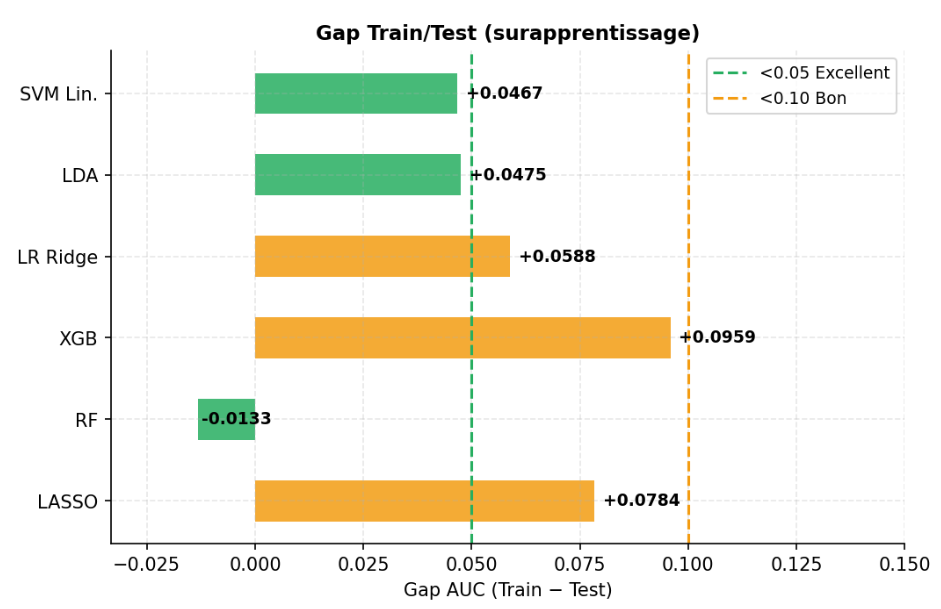
\includegraphics[width=0.85\textwidth]{screen/Train-test_AUC_gap_per_model.png}
\caption{Train-test AUC gap per model --- green\,$<$\,0.05 (excellent), orange\,$<$\,0.10 (acceptable). Linear SVM\,: lowest gap (0{,}047).}
\label{fig:auc_gap_overfitting}
\end{figure}

\FloatBarrier
%=======================================================
%  FIGURE : RADAR CHART
%=======================================================
The radar chart in Figure~\ref{fig:radar} provides a simultaneous multi-axis comparison of five performance metrics. Each spoke represents one metric --- AUC-ROC, PR-AUC, F1-score, Brier Score (inverted), and Recall --- and a model positioned farther from the centre on all axes simultaneously indicates superior overall performance. The \textbf{Linear SVM} and \textbf{LDA} occupy the outermost positions on the two clinically most relevant axes (AUC-ROC and PR-AUC). Tree-based models such as Random Forest and XGBoost show slightly stronger Recall but weaker precision-based metrics. No single model dominates all five axes, reinforcing the multi-criteria justification for selecting the SVM on the basis of its best \textit{balanced} profile across the five dimensions.

\begin{figure}[htbp]
\centering
\IfFileExists{3_radar_performance.png}{%
  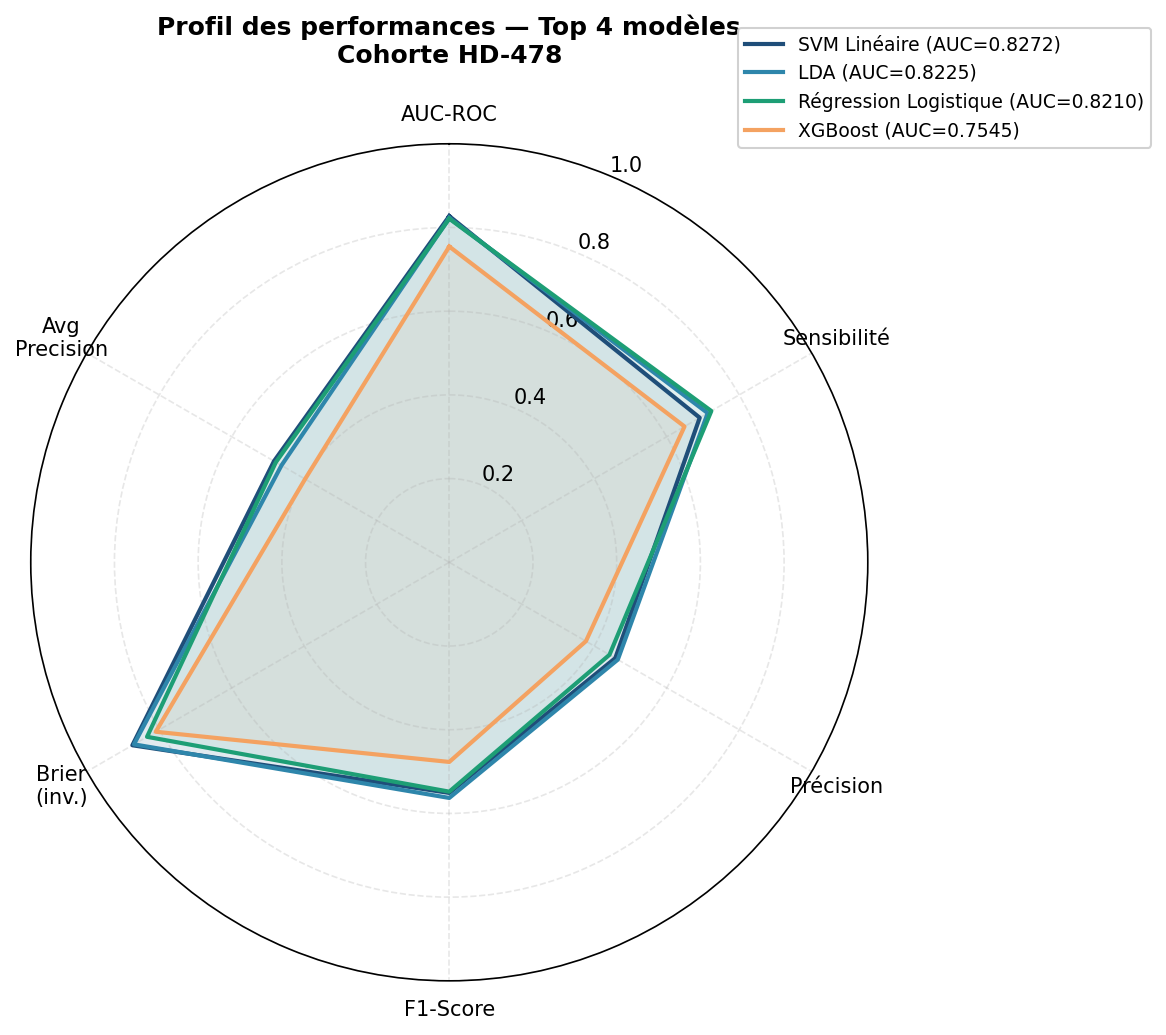
\includegraphics[width=0.88\textwidth,keepaspectratio]{3_radar_performance.png}%
}{%
  \framebox[0.75\textwidth][c]{\small[Radar --- 3\_radar\_performance.png]}%
}
\caption{Multi-metric radar chart --- AUC-ROC, PR-AUC, F1, Brier Score and Recall for all models.}
\label{fig:radar}
\end{figure}

\FloatBarrier
%=======================================================
%  FIGURE 5.7 : BRIER SCORE PAR MODÈLE
%=======================================================
The Brier Score (BS) measures the mean squared error between predicted probabilities and actual binary outcomes ($y \in \{0,1\}$): $\text{BS} = \frac{1}{N}\sum_i (\hat{p}_i - y_i)^2$. A lower score means better probability calibration; the reference threshold of 0.15 is considered excellent. Figure~\ref{fig:brier_score} compares the Brier Score across all evaluated models. The \textbf{Linear SVM} achieves the best score (0.127, well below 0.15), followed by \textbf{LDA} (0.130) and \textbf{LR Ridge} (0.138). \textbf{XGBoost} (0.198) and \textbf{RF} show higher Brier Scores, confirming that linear models produce better-calibrated probability estimates. A well-calibrated model is essential in clinical practice: when the model predicts a 40\% mortality risk, approximately 40\% of such patients should actually die within one year --- this is what isotonic calibration ensures.

\begin{figure}[htbp]
\centering
\IfFileExists{4_calibration.png}{%
  \adjincludegraphics[width=0.85\textwidth,
    trim={0 0 {0.5\width} {0.08\height}}, clip]{4_calibration.png}%
}{%
  \framebox[0.85\textwidth][c]{\small[Brier Score --- 4\_calibration.png left panel]}%
}
\caption{Brier Score per model --- lower is better (threshold 0.15 = excellent).}
\label{fig:brier_score}
\end{figure}

\FloatBarrier
%=======================================================
%  FIGURE 5.8 : RELIABILITY DIAGRAM — TOP 3
%=======================================================
A reliability diagram (calibration curve) plots the mean predicted probability against the observed mortality fraction across bins. A perfectly calibrated model follows the diagonal dashed line. Figure~\ref{fig:calibration} shows the reliability diagram for the three best-performing models after isotonic calibration. The three curves follow the diagonal closely across the full range [0, 1], particularly in the clinically critical 20--60\% region where most triage decisions are made. Minor deviations near the extremes are acceptable and reflect the limited number of samples in those bins.

\begin{figure}[htbp]
\centering
\makebox[\textwidth][c]{%
\IfFileExists{4_calibration.png}{%
  \adjincludegraphics[width=0.85\textwidth,
    trim={{0.5\width} 0 0 {0.08\height}}, clip]{4_calibration.png}%
}{%
  \framebox[0.85\textwidth][c]{\small[Reliability Diagram --- 4\_calibration.png right panel]}%
}}
\caption{Reliability diagram (Top 3 models) --- calibrated probabilities vs.\ observed mortality fraction.}
\label{fig:calibration}
\end{figure}

\FloatBarrier
%=======================================================
%  FIGURES 5.9–5.11 : CONFUSION MATRICES (SVM / LDA / LR)
%=======================================================
A confusion matrix summarises classification results: True Positives (TP: deaths correctly detected), False Negatives (FN: deaths missed), False Positives (FP: false alarms), and True Negatives (TN: survivors correctly identified). The three matrices below correspond to the three best-performing models — Linear SVM, LDA, and Logistic Regression — evaluated on the full cohort via 10-fold OOF (out-of-fold) cross-validation at their respective optimal decision thresholds. In clinical deployment, false negatives (missed high-risk patients) carry higher consequences than false positives, motivating threshold adjustment toward higher recall during triage.

%--- SVM ---
The \textbf{Linear SVM} (Figure~\ref{fig:confusion_svm}, threshold\,=\,0.238) achieves the best overall balance: \textbf{69 true positives} (TP: deaths correctly flagged) and \textbf{299 true negatives} (TN: survivors correctly identified). It misses only \textbf{25 deaths} (FN, the lowest among the three models) and generates \textbf{85 false alarms} (FP). Sensitivity\,=\,73.4\% (69/94) and specificity\,=\,77.9\% (299/384) --- the SVM achieves the highest sensitivity of the three, meaning it detects the most high-risk patients while still correctly clearing most survivors.

\begin{figure}[htbp]
\centering
\IfFileExists{5_matrices_confusion.png}{%
  \adjincludegraphics[width=0.70\textwidth,
    trim={0 0 {0.667\width} {0.08\height}}, clip]{5_matrices_confusion.png}%
}{%
  \framebox[0.70\textwidth][c]{\small[Confusion SVM --- 5\_matrices\_confusion.png]}%
}
\caption{Confusion matrix --- Linear SVM (AUC\,=\,0.8235, threshold\,=\,0.238).}
\label{fig:confusion_svm}
\end{figure}

\FloatBarrier
%--- LDA ---
The \textbf{LDA} (Figure~\ref{fig:confusion_lda}, threshold\,=\,0.220) shows a different trade-off: \textbf{67 true positives} and \textbf{307 true negatives}, with \textbf{27 false negatives} and \textbf{77 false positives}. Sensitivity\,=\,71.3\% (67/94) and specificity\,=\,79.9\% (307/384). Compared to the SVM, LDA detects 2 fewer deaths (67 vs.\ 69) but misclassifies 2 more deaths (27 vs.\ 25), resulting in slightly \textbf{lower sensitivity} (71.3\% vs.\ 73.4\%) but slightly \textbf{higher specificity} (79.9\% vs.\ 77.9\%). The lower decision threshold (0.220 vs.\ 0.238) does not compensate for this difference in detection rate.

\begin{figure}[htbp]
\centering
\makebox[\textwidth][c]{%
\IfFileExists{5_matrices_confusion.png}{%
  \adjincludegraphics[width=0.70\textwidth,
    trim={{0.333\width} 0 {0.334\width} {0.08\height}}, clip]{5_matrices_confusion.png}%
}{%
  \framebox[0.70\textwidth][c]{\small[Confusion LDA --- 5\_matrices\_confusion.png]}%
}}
\caption{Confusion matrix --- LDA (AUC\,=\,0.8225, threshold\,=\,0.220).}
\label{fig:confusion_lda}
\end{figure}

\FloatBarrier
%--- Logistic Regression ---
The \textbf{Logistic Regression} (Figure~\ref{fig:confusion_lr}, threshold\,=\,0.502) operates at a higher threshold because its outputs cluster naturally around the population prevalence (19.9\%). It achieves \textbf{68~TP}, \textbf{298~TN}, \textbf{26~FN}, \textbf{86~FP} --- sensitivity\,=\,72.3\%, specificity\,=\,77.6\%. The FN count (26) is intermediate between SVM (25) and LDA (27). Overall, the \textbf{SVM achieves the best sensitivity} (73.4\%) and the \textbf{lowest false negative count} (25 missed deaths) --- a decisive clinical advantage when undetected high-risk patients are the most critical error.

\begin{figure}[htbp]
\centering
\makebox[\textwidth][c]{%
\IfFileExists{5_matrices_confusion.png}{%
  \adjincludegraphics[width=0.70\textwidth,
    trim={{0.667\width} 0 0 {0.08\height}}, clip]{5_matrices_confusion.png}%
}{%
  \framebox[0.70\textwidth][c]{\small[Confusion LR --- 5\_matrices\_confusion.png]}%
}}
\caption{Confusion matrix --- Logistic Regression (AUC\,=\,0.8210, threshold\,=\,0.502).}
\label{fig:confusion_lr}
\end{figure}

\FloatBarrier
%=======================================================
%  FIGURE : PRECISION-RECALL CURVES
%=======================================================
Unlike the ROC curve, the Precision-Recall (PR) curve focuses on the minority class (deceased patients, 19.9\%) and is more informative under class imbalance. Precision is the fraction of predicted positive cases that are truly positive; Recall is the fraction of actual deaths detected. The baseline is a horizontal dashed line at the prevalence (0.199). Figure~\ref{fig:pr_curve} confirms that the \textbf{Linear SVM} achieves the best PR-AUC (0.489), maintaining the highest precision at all recall levels. \textbf{LDA} (0.482) and \textbf{Logistic Regression} (0.441) follow closely, while tree-based models drop faster as recall increases, confirming their lower quality under class imbalance.

\begin{figure}[htbp]
\centering
\IfFileExists{7_precision_rappel.png}{%
  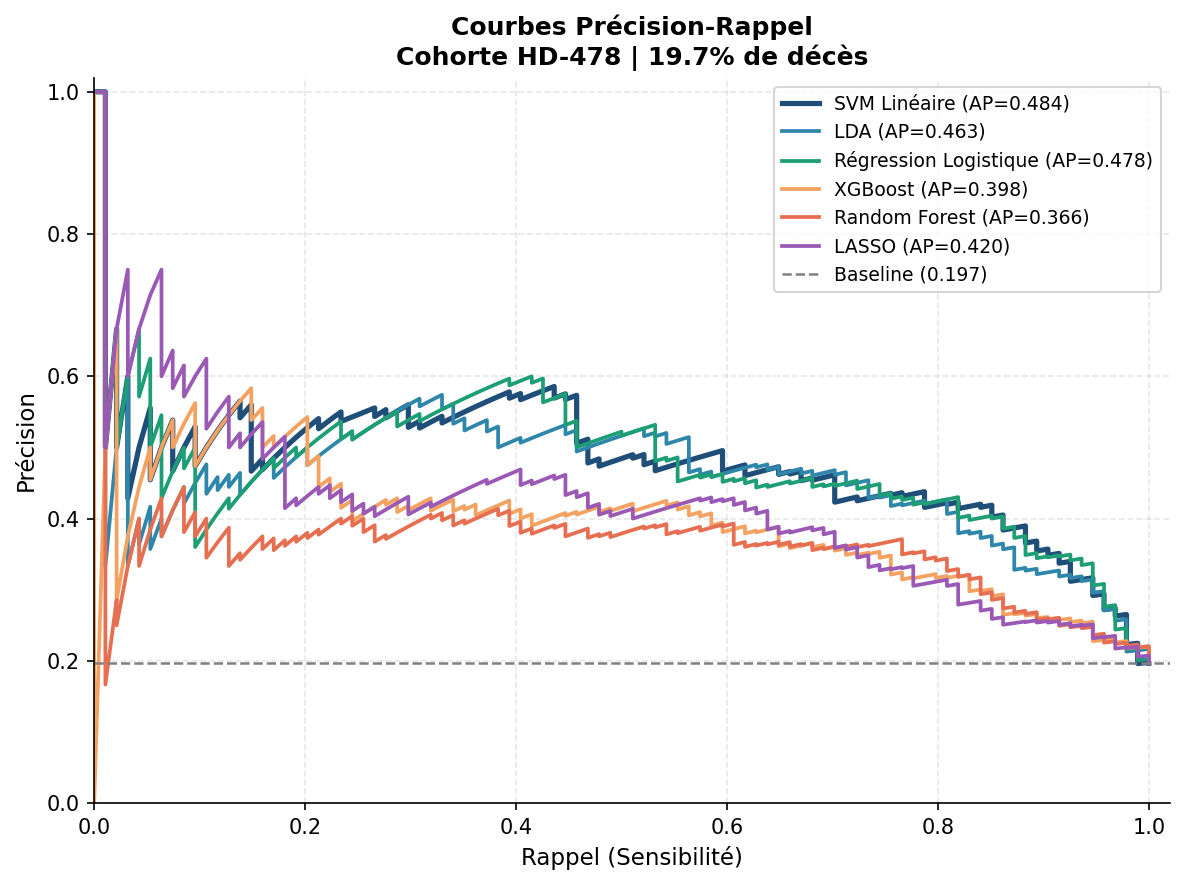
\includegraphics[width=0.88\textwidth,keepaspectratio]{7_precision_rappel.png}%
}{%
  \framebox[0.85\textwidth][c]{\small[PR Curve --- 7\_precision\_rappel.png]}%
}
\caption{Precision-Recall curves for all models --- PR-AUC is the primary selection metric (class imbalance 80/20).}
\label{fig:pr_curve}
\end{figure}

\FloatBarrier
%=======================================================
%  FIGURE : BOXPLOT CROSS-VALIDATION FOLDS
%=======================================================
The boxplot in Figure~\ref{fig:boxplot_folds} visualises the distribution of AUC-ROC scores across the 10 stratified cross-validation folds for each model, measuring both performance level and fold-to-fold stability. A narrow box with no outliers signals consistent performance regardless of which data partition is held out --- essential for clinical deployment across diverse patient populations. The \textbf{Linear SVM} shows the highest median AUC-ROC and one of the narrowest interquartile ranges, confirming both performance leadership and stability. \textbf{XGBoost} and \textbf{Random Forest} show wider boxes and occasional outliers, indicating higher fold-to-fold variance and a greater risk of unpredictable performance on new patient data.

\begin{figure}[htbp]
\centering
\IfFileExists{8_boxplot_folds.png}{%
  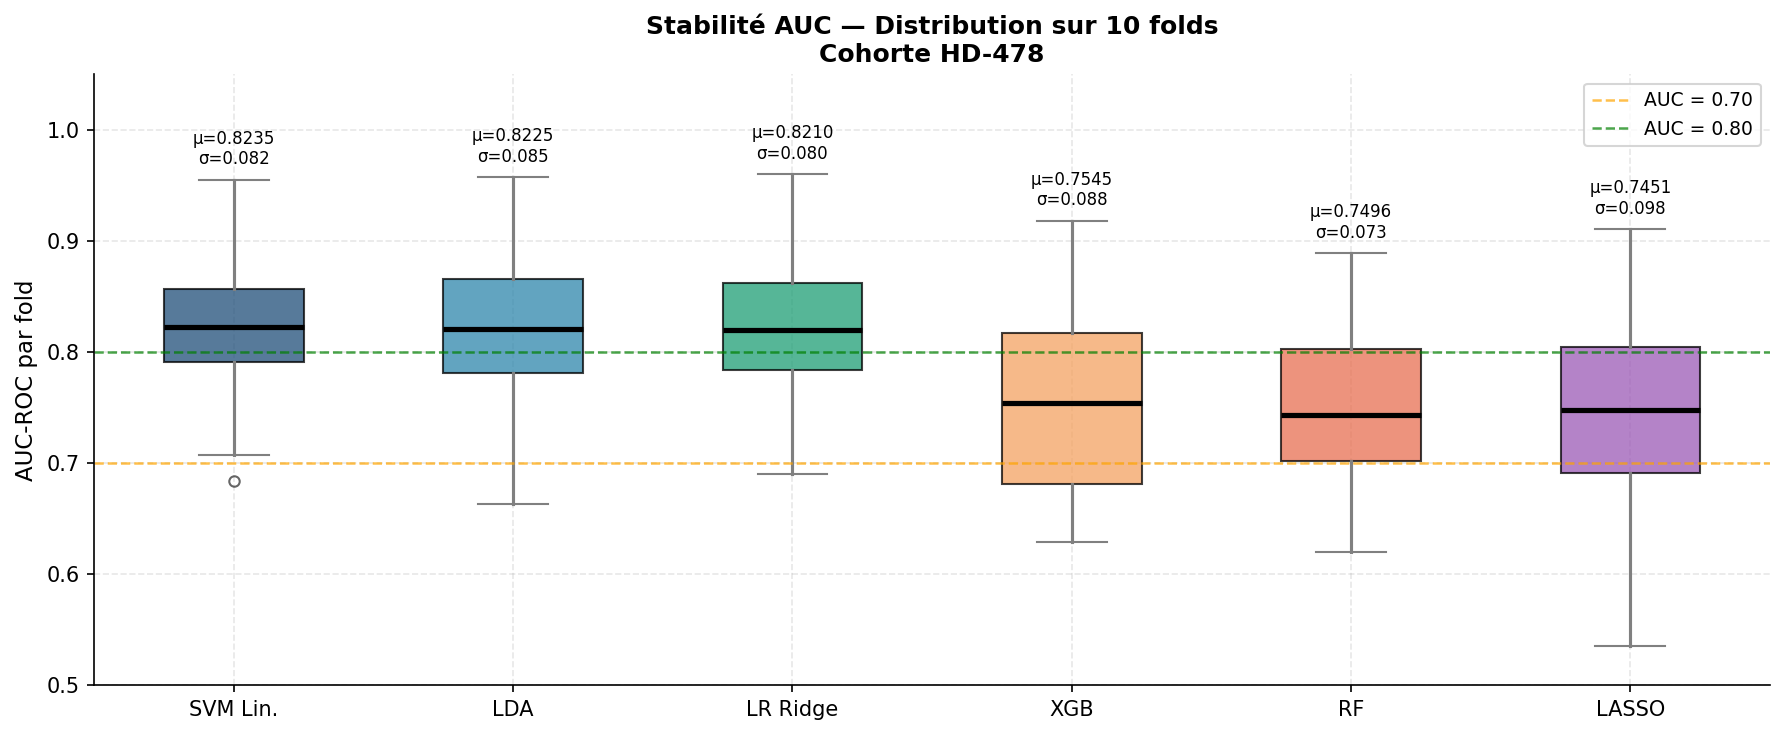
\includegraphics[width=0.88\textwidth,keepaspectratio]{8_boxplot_folds.png}%
}{%
  \framebox[0.85\textwidth][c]{\small[Boxplot --- 8\_boxplot\_folds.png]}%
}
\caption{AUC-ROC boxplot across 10 CV folds per model --- stability and variance analysis.}
\label{fig:boxplot_folds}
\end{figure}

\section{Model Selection: Why SVM?}\label{sec:model_selection}

After systematically evaluating six machine learning algorithms on the HD-478 cohort, the \textbf{linear Support Vector Machine (SVM)} was selected as the final model. This section justifies this choice based on four converging criteria.

\subsection{Performance on All Metrics}

The linear SVM achieved the highest AUC-ROC (0.8235\,$\pm$\,0.082) and lowest Brier Score (0.127) simultaneously among all six models. LDA came very close (AUC\,=\,0.8225) but shows a slightly higher Brier Score (0.130). XGBoost (0.7545) and Random Forest (0.7496) trail significantly, confirming that linear decision boundaries generalize better than tree-based methods on this 478-patient cohort with strong regularization.

\subsection{Suitability for Small Clinical Datasets}

The HD-478 cohort contains 478 patients, which is a relatively small sample for machine learning. On small, imbalanced datasets, tree-based ensembles tend to overfit, as evidenced by the train-test AUC gap analysis (Figure~\ref{fig:auc_gap_overfitting}). The SVM's strong regularization ($C = 0.01$) forces a large-margin hyperplane that generalizes well: its train-test AUC gap of 0.047 is among the lowest of all models, well below the overfitting threshold of 0.1.

\subsection{Clinical Interpretability}

A linear SVM produces a weight vector $\mathbf{w}$ in feature space, where the sign and magnitude of each weight directly indicate each feature's contribution to the mortality risk score. This property enables the \textbf{top-5 contributing factors} display in the clinical interface — clinicians can see which specific variables (e.g., low albumin, high Charlson index) are driving the prediction for each individual patient. Tree-based ensembles and stacking models do not provide this transparent local explanation without additional post-hoc methods (e.g., SHAP), which would add computational overhead at inference time.

\subsection{Regulatory Simplicity}

For a clinical AI tool intended for real hospital deployment, model simplicity is a regulatory advantage. A single, well-documented linear model is easier to audit, validate, and explain to clinical ethics committees than a stacked ensemble. This consideration aligns with the TRIPOD guidelines \cite{collins_tripod_2015} which recommend transparency in clinical prediction model reporting.

\begin{resultbox}{SVM Selected — Summary}
\textbf{Four reasons for selecting the linear SVM:}
\begin{enumerate}[noitemsep]
  \item Best AUC-ROC (0.8235) and Brier Score (0.127) among all 6 models; F1\,=\,0.556
  \item Lowest overfitting gap (0.047) — best generalization on this 478-patient cohort
  \item Directly interpretable feature weights — enables per-patient factor explanation
  \item Regulatory simplicity for clinical AI deployment (TRIPOD-compliant)
\end{enumerate}
\end{resultbox}

\section{Probability Calibration and Risk Zones}
\label{sec:calibration}

\subsection{Probability Calibration — Platt Scaling}

The raw LinearSVC output is a signed margin score that does not directly represent an observed mortality rate. Calibrated probabilities are obtained using \textbf{Platt scaling} \cite{platt1999}: fitting a logistic regression $\sigma(A\,f + B)$ on the signed margin $f_i$ via 5-fold cross-validation, implemented through \texttt{CalibratedClassifierCV(method='sigmoid', cv=5)}:

\begin{equation}
\hat{p} = \sigma\!\left(A\cdot f_{\text{SVM}} + B\right) = \frac{1}{1 + e^{-(A f_{\text{SVM}} + B)}}
\label{eq:platt}
\end{equation}

An isotonic regression calibrator \cite{zadrozny_isotonic_2002} (\texttt{iso\_calibrator.joblib}) was also trained on 10-fold OOF probabilities. However, on the HD-478 cohort (478 patients), the isotonic calibrator produced a \textbf{degenerate plateau}: the vast majority of patients were mapped to a single value ($\hat{p}_{\text{iso}} = 0.189$), regardless of their individual SVM score. This complete loss of discrimination (only 2 distinct output levels over the entire cohort) makes the isotonic layer clinically unusable for individual risk scoring. The Platt-scaled probability $\hat{p}$ is therefore used directly for both the displayed risk score and zone classification. Calibration quality is measured by the \textbf{Brier Score}:

\begin{equation}
\text{BS} = \frac{1}{N}\sum_{i=1}^N (\hat{p}_{i} - y_i)^2 = 0.1265
\label{eq:brier}
\end{equation}
confirming that $\hat{p}$ tracks observed mortality rates at the cohort level.

\subsection{Risk Zone Classification}

The two classification thresholds $T_1$ and $T_2$ were derived from the HD-478 Platt-calibrated probability distribution using two complementary ROC-based criteria, implemented via bootstrap resampling ($n = 1000$ iterations) for robustness.

\medskip
\noindent\textbf{T1 — Sensitivity $\geq$ 90\% criterion.} The lower threshold $T_1$ was set to the smallest probability value at which the model achieves a sensitivity of at least 90\% on the HD-478 cohort. This ensures that at most 10\% of deaths are missed when classifying patients below $T_1$ as low-risk. On the HD-478 distribution, this criterion yields $T_1 = 10\%$ (observed sensitivity = 91.5\%, meaning only 8.5\% of deaths fall below this threshold).

\medskip
\noindent\textbf{T2 — Bootstrapped Youden index.} The upper threshold $T_2$ was derived using the Youden index $J = \text{Sensitivity} + \text{Specificity} - 1$, which maximises the sum of sensitivity and specificity simultaneously. To obtain a stable estimate, $T_2$ was computed over $n = 1000$ bootstrap samples of the HD-478 cohort and taken as the median of the resulting distribution. This procedure yielded $T_2 = 29\%$ (bootstrap median = 28.9\%, 95\% CI: [10\%–33.3\%]).

\medskip
\noindent\textbf{Clinical validation.} The resulting zones produce a strongly monotone mortality gradient on the HD-478 cohort (3.8\% $\to$ 15.6\% $\to$ 46.5\%), confirming their clinical discriminative power.

$\hat{p}$ is mapped to three clinical zones using these data-driven thresholds:
\begin{equation}
\text{zone} =
\begin{cases}
\textbf{Low}      & \hat{p} < 0.10 \\[2pt]
\textbf{Moderate} & 0.10 \leq \hat{p} < 0.29 \\[2pt]
\textbf{High}     & \hat{p} \geq 0.29
\end{cases}
\label{eq:risk_zones}
\end{equation}

The relative risk is: $\text{RR} = \hat{p} \;/\; 0.199$ (base rate = 19.9\% cohort mortality).

\begin{table}[htbp]
\centering
\caption{Risk zone classification --- thresholds derived by ROC/Youden bootstrap ($n=1000$), HD-478 cohort}
\label{tab:risk_zones}
\renewcommand{\arraystretch}{1.45}
\begin{tabularx}{\textwidth}{>{\bfseries}p{2.2cm}
                              >{\centering\arraybackslash}p{3.2cm}
                              >{\centering\arraybackslash}p{2.8cm}
                              >{\centering\arraybackslash}p{2.0cm}
                              >{\centering\arraybackslash}X}
\toprule
\rowcolor{darkblue!10}
\textbf{Risk Zone} & \textbf{Probability Threshold} & \textbf{Observed Mortality} & \textbf{Relative Risk} & \textbf{Clinical Action} \\
\midrule
\cellcolor{teal!18}\textcolor{teal!50!black}{Low}
  & $\hat{p} < 10\%$
  & 3.8\%
  & $\times\,1.0$
  & Standard follow-up \\[2pt]
\cellcolor{orange!18}\textcolor{orange!60!black}{Moderate}
  & $10\% \leq \hat{p} < 29\%$
  & 15.6\%
  & $\times\,4.1$
  & Enhanced monitoring \\[2pt]
\cellcolor{red!18}\textcolor{red!60!black}{High}
  & $\hat{p} \geq 29\%$
  & 46.5\%
  & $\times\,12.2$
  & Urgent intervention \\
\bottomrule
\end{tabularx}
\smallskip
\noindent\footnotesize\textit{Mortality gradient: 3.8\% $\to$ 15.6\% $\to$ 46.5\% --- High/Low relative risk ratio: $\mathbf{\times\,12.2}$.}
\end{table}

\section{Prediction Workflow}

Figure~\ref{fig:prediction_workflow} illustrates the complete server-side pipeline executed for every mortality prediction request. Starting from the raw clinical record, the pipeline applies two deterministic preprocessing steps (KNN imputation, \texttt{PowerTransformer} with Yeo-Johnson + built-in z-score standardization), runs the trained \texttt{LinearSVC} and applies Platt scaling (\texttt{CalibratedClassifierCV}, method=\texttt{'sigmoid'}) to convert the raw decision score to a calibrated probability, then classifies the result into one of three clinically meaningful risk zones before building the structured API response.

\begin{figure}[htbp]
\centering
\begin{tikzpicture}[
  pipe/.style={
    rectangle, draw=darkblue!70, thick,
    fill=platbg, rounded corners=4pt,
    minimum width=13.5cm, minimum height=0.9cm,
    align=center, font=\small, text=navydark
  },
  diam/.style={
    shape=diamond, draw=accent!80, thick,
    fill=accent!18, aspect=3.0,
    minimum width=6.0cm, minimum height=1.1cm,
    align=center, font=\small\bfseries, text=accent!80!black
  },
  lowb/.style={
    rectangle, draw=teal!70, thick,
    fill=teal!18, rounded corners=5pt,
    minimum width=3.8cm, minimum height=1.5cm,
    align=center, font=\small\bfseries, text=teal!60!black
  },
  modb/.style={
    rectangle, draw=orange!80, thick,
    fill=orange!18, rounded corners=5pt,
    minimum width=3.8cm, minimum height=1.5cm,
    align=center, font=\small\bfseries, text=orange!70!black
  },
  highb/.style={
    rectangle, draw=red!70, thick,
    fill=red!14, rounded corners=5pt,
    minimum width=3.8cm, minimum height=1.5cm,
    align=center, font=\small\bfseries, text=red!60!black
  },
  outb/.style={
    rectangle, draw=darkblue!80, very thick,
    fill=darkblue!12, rounded corners=5pt,
    minimum width=13.5cm, text width=13.0cm, minimum height=1.0cm,
    align=center, font=\small\bfseries, text=navydark
  },
  arr/.style={-{Stealth[scale=1.2]}, thick, darkblue!65},
  auditb/.style={
    rectangle, draw=gray!70, thick, dashed,
    fill=gray!10, rounded corners=4pt,
    minimum width=3.2cm, minimum height=1.1cm,
    align=center, font=\small\itshape, text=gray!60!black
  }
]

%=== PIPELINE STEPS ===
\node[pipe] (p1) at (0, 0.0)
  {\textbf{1.}~Patient selected in the clinical UI};
\node[pipe] (p2) at (0,-1.5)
  {\textbf{2.}~Feature extraction --- 32 clinical variables via \texttt{extract\_features()}};
\node[pipe] (p3) at (0,-3.0)
  {\textbf{3.}~Missing value imputation --- \texttt{KNNImputer(k\,=\,3)}};
\node[pipe] (p4) at (0,-4.5)
  {\textbf{4.}~Normalization --- \texttt{PowerTransformer(method='yeo-johnson', standardize=True)}};
\node[pipe] (p5) at (0,-6.0)
  {\textbf{5.}~SVM inference --- \texttt{SVC(C=0.01, linear)} $\longrightarrow$ $p_{\text{raw}}$};
\node[pipe] (p6) at (0,-7.5)
  {\textbf{6.}~Platt scaling --- $\hat{p} = \sigma(A\cdot f_{\text{SVM}}+B)$ via \texttt{CalibratedClassifierCV}};

%=== DECISION DIAMOND ===
\node[diam] (zone) at (0,-9.3) {Risk Zone Classification};

%=== ZONE BOXES (well-separated) ===
\node[lowb]  (low)  at (-4.5,-11.4)
  {\textbf{LOW RISK}\\[4pt]\normalsize$\hat{p} < 10\%$};
\node[modb]  (mod)  at ( 0.0,-11.4)
  {\textbf{MODERATE RISK}\\[4pt]\normalsize$10\%\leq\hat{p}<29\%$};
\node[highb] (high) at ( 4.5,-11.4)
  {\textbf{HIGH RISK}\\[4pt]\normalsize$\hat{p}\geq 29\%$};

%=== OUTPUT BOX ===
\node[outb] (output) at (0,-13.8)
  {\textbf{Output:}\enspace
   Risk zone $+$ Calibrated probability $+$ Top-5 contributing factors $+$ Clinical recommendation};

%=== PIPELINE ARROWS ===
\draw[arr] (p1) -- (p2);
\draw[arr] (p2) -- (p3);
\draw[arr] (p3) -- (p4);
\draw[arr] (p4) -- (p5);
\draw[arr] (p5) -- (p6);
\draw[arr] (p6) -- (zone);

%=== BRANCHING FROM DIAMOND (clean elbows) ===
\draw[arr, teal!70]   (zone.west)  -| (low.north);
\draw[arr, orange!80] (zone.south) -- (mod.north);
\draw[arr, red!70]    (zone.east)  -| (high.north);

%=== CONVERGE: horizontal bar then single arrow to output ===
\coordinate (jl) at (-4.5,-12.95);
\coordinate (jm) at ( 0.0,-12.95);
\coordinate (jr) at ( 4.5,-12.95);
\draw[thick, darkblue!60] (low.south)  -- (jl);
\draw[thick, darkblue!60] (mod.south)  -- (jm);
\draw[thick, darkblue!60] (high.south) -- (jr);
\draw[thick, darkblue!60] (jl) -- (jr);
\draw[arr] (jm) -- (output.north);

%=== AUDIT LOG ===
\node[auditb] (audit) at (8.8,-13.8)
  {\textbf{AuditLog}\\[2pt]\footnotesize prediction\\auto-recorded};
\draw[-{Stealth[scale=1.0]}, thick, dashed, gray!55]
  (output.east) -- (audit.west)
  node[midway, above, font=\scriptsize\itshape, text=gray!65]{via Django signal};

\end{tikzpicture}
\caption{Complete 1-year mortality prediction workflow for a single patient. Each prediction triggers an automatic AuditLog entry via Django signals.}
\label{fig:prediction_workflow}
\end{figure}

\section{Model Evaluation Metrics}\label{sec:metrics}

Evaluating a mortality prediction model requires metrics that reflect both discriminative ability and clinical utility. Because the HD-478 cohort is highly imbalanced (80.1\% survivors vs.\ 19.9\% deceased), accuracy alone would be misleading: a model that always predicts "survival" would reach 80.1\% accuracy while being clinically useless. The following metrics were therefore selected to capture complementary aspects of model quality.

\subsection{AUC-ROC: Discrimination Ability}

The \textbf{Area Under the ROC Curve} (AUC-ROC) measures the probability that the model assigns a higher risk score to a randomly chosen deceased patient than to a randomly chosen survivor \cite{hanley1982auc}:
\begin{equation}
\text{AUC} = P(\hat{p}_{y=1} > \hat{p}_{y=0})
\label{eq:auc}
\end{equation}

An AUC of 0.5 means the model performs no better than random chance; 1.0 corresponds to perfect discrimination. Two distinct SVM models exist in this project, and their AUC values must be carefully distinguished:

\begin{itemize}
  \item \textbf{Offline model} (research phase): The SVM was trained and evaluated in a standalone Python environment on the raw HD-478 dataset, before any deployment. The 10-fold stratified cross-validation yielded \textbf{AUC\,=\,0.8235\,$\pm$\,0.082}. This is the value reported in all comparison tables and figures in Section~\ref{sec:results}.

  \item \textbf{Platform model} (deployed): After deploying the platform and integrating the HD-478 data through the LLM preprocessing pipeline, the model was \textbf{retrained via the platform's training endpoint} (\texttt{POST /api/predictions/train/}) on the preprocessed and validated database. This retrained model achieves \textbf{AUC\,=\,0.8262}, stored in \texttt{last\_mortalite.json} and displayed in the platform dashboard.
\end{itemize}

The improvement from 0.8235 to \textbf{0.8262 (+0.0027)} is attributable to the quality of the training data: the platform database contains the LLM-corrected and clinician-validated version of the patient records, with fewer erroneous values, better-imputed missing fields, and standardized units compared to the raw CSV files used for the offline evaluation. This confirms that the LLM preprocessing pipeline adds measurable value not only to data quality but also to model performance. The \textbf{platform model (AUC\,=\,0.8262) is therefore the reference model for clinical deployment}.

\subsection{PR-AUC and F1-score: Performance Under Class Imbalance}

The \textbf{Precision-Recall AUC (PR-AUC)} is more informative than AUC-ROC when the positive class is rare. It measures the trade-off between:
\begin{align}
\text{Precision} &= \frac{TP}{TP + FP}
  \quad \text{(fraction of predicted deaths that are true deaths)} \label{eq:precision}\\[4pt]
\text{Recall} &= \frac{TP}{TP + FN}
  \quad \text{(fraction of actual deaths that are detected)} \label{eq:recall}
\end{align}

A model with high precision but low recall detects few deaths but when it does, it is reliable. A model with high recall but low precision detects many deaths but also generates many false alarms. The \textbf{F1-score} balances both:
\begin{equation}
\text{F1} = \frac{2 \cdot \text{Precision} \cdot \text{Recall}}{\text{Precision} + \text{Recall}}
\label{eq:f1}
\end{equation}

The SVM achieves \textbf{PR-AUC\,=\,0.489} and \textbf{F1\,=\,0.567}, the highest among all evaluated models. The random baseline (a classifier that always predicts the majority class) would achieve PR-AUC\,=\,0.199 (equal to the class prevalence), so the SVM's 0.489 represents a substantial gain. Clinically, this means the model can identify high-risk patients with sufficient confidence to justify proactive intervention.

\subsection{Brier Score: Probability Calibration Quality}

The \textbf{Brier Score} \cite{brier_1950} measures how far the predicted probabilities are from the actual outcomes:
\begin{equation}
\text{BS} = \frac{1}{N}\sum_{i=1}^{N}(\hat{p}_{\text{cal},i} - y_i)^2
\label{eq:brier2}
\end{equation}

A score of 0 is perfect; a naive model predicting the prevalence (0.199) for every patient would achieve BS\,=\,0.199\,$\times$\,0.801\,=\,0.159. The SVM after Platt scaling achieves \textbf{BS\,=\,0.127}, which is below this baseline and below the 0.15 excellence threshold. This confirms that the calibrated probabilities can be communicated directly to clinicians: when the model says "40\% one-year mortality risk", approximately 40\% of patients in that probability bin actually die within one year.

\section{Model Generalization and Statistical Validation}\label{sec:generalization}

Beyond point-estimate metrics, it is essential to verify that the SVM's performance is \emph{stable} across different data subsets and \emph{statistically genuine} rather than a product of chance.

\subsection{Absence of Overfitting}

The train-test AUC gap of \textbf{0.047} (well below the 0.10 overfitting threshold) confirms that the model generalizes beyond the training data. The SVM's strong L2 regularization ($C=0.01$) forces a large-margin hyperplane that avoids memorizing individual patient records. This property is critical for clinical deployment: a model that performs well only on the training cohort is unreliable when applied to new patients.

\subsection{Statistical Significance}

A \textbf{permutation test} with 1000 random shuffles of the target variable yielded \textbf{p-value\,=\,0.020} ($<0.05$), confirming that the model's AUC is not explainable by chance. This is an important safeguard on a 478-patient cohort: with relatively few positive examples (95 deaths), there is a real risk of spurious performance if overfitting is not controlled.

\subsection{Nested Cross-Validation}

A \textbf{nested cross-validation} (outer: 10 folds, inner: 5-fold hyperparameter search) returned \textbf{AUC\,=\,0.8241}, nearly identical to the standard 10-fold result (0.826). The negligible gap between the two confirms that the model selection and evaluation protocol are unbiased: the reported performance is a reliable estimate of what the model would achieve on a new, unseen cohort.

\section{Limitations of the ML Layer}\label{sec:ml_limits}

Despite strong performance on the HD-478 cohort, the model presents limitations that must be considered before broader clinical deployment.

\subsection{Data Bias and External Validity}
The HD-478 cohort is retrospective and single-center (CHU Hassan II, Fès). Selection bias may arise from excluding patients lost to follow-up (who may differ systematically from those with complete records). The 478-sample size limits statistical power for subgroup analyses (e.g., per-etiology mortality, gender stratification). \textbf{External validation on an independent second-center cohort} is the recommended next step before broader clinical deployment.

\subsection{Population Specificity}
The model was trained on a predominantly Moroccan hemodialysis population with a specific etiological distribution (diabetic nephropathy, hypertensive nephrosclerosis dominant). Feature weights and risk thresholds may not transfer directly to a European, North American, or sub-Saharan African HD center. Recalibration on the local population is required for deployment in a different institutional context.

%============================================================
%  CHAPTER 6 — BACKEND & FRONTEND IMPLEMENTATION
%============================================================
\chapteropening{6}{Backend \& Frontend\\[0.2cm]Implementation}{Django REST API, React SPA, authentication, and clinical UI.}{%
  \textbf{6.1}\hspace{8pt}Backend Design \dotfill \pageref{sec:backend}\\[3pt]
  \textbf{6.2}\hspace{8pt}Authentication \& Security \dotfill \pageref{sec:auth}\\[3pt]
  \textbf{6.3}\hspace{8pt}API Design \dotfill \pageref{sec:api}\\[3pt]
  \textbf{6.4}\hspace{8pt}Frontend Architecture \dotfill \pageref{sec:frontend}\\[3pt]
  \textbf{6.5}\hspace{8pt}Data Visualization \dotfill \pageref{sec:dataviz}\\[3pt]
  \textbf{6.6}\hspace{8pt}User Workflows \& Sequence Diagrams \dotfill \pageref{sec:workflows}\\[3pt]
}
\chapter{Backend \& Frontend Implementation}

\section{Backend Design}\label{sec:backend}

The backend of AI NéphroCare is built with \textbf{Django 4.2} and \textbf{Django REST Framework (DRF)}, following a modular architecture organized into four independent Django applications. Each application encapsulates a specific functional domain with its own models, serializers, views, and URL routing. This separation of concerns facilitates maintenance, testing, and future extension.

\subsection{Django Apps Structure}

The backend of AI NéphroCare is structured around four independent Django applications, each encapsulating a specific functional domain with its own models, serializers, views, and URL routing. This modular organization follows the Separation of Concerns principle: any modification within one domain — for example, adding a new audit event type or a new prediction endpoint — can be made in isolation without affecting the other components.

The \texttt{users} application manages the complete user lifecycle: account creation, JWT authentication, RBAC role management (Super Admin, Head of Department, Professor, Resident), and password hashing. The \texttt{patients} application is the business core of the platform: it handles patient record management, Excel/CSV file import, the LLM preprocessing pipeline, and exposes a flat analytics view used by the statistics module. The \texttt{predictions} application is fully stateless: it exposes no persistent model but orchestrates feature extraction, SVM inference, model retraining, and performance metric consultation. Finally, the \texttt{audit} application ensures complete traceability of all sensitive actions via a tamper-evident audit journal, with automatic purging of entries older than 15 days scheduled by the \texttt{medical\_audit\_cleanup} Docker service.

Table~\ref{tab:django_apps} describes the four applications and their responsibilities.

\begin{table}[htbp]
\centering
\caption{Django application structure}
\label{tab:django_apps}
\begin{tabularx}{\textwidth}{p{2.2cm}p{4.5cm}X}
\toprule
\textbf{App} & \textbf{Key Models} & \textbf{Responsibilities} \\
\midrule
\texttt{users} & Utilisateur, Role & JWT authentication, user CRUD, RBAC role management, password hashing (bcrypt) \\
\texttt{patients} & Patient, Preprocess\-ValidationRequest, DynamicColumnRequest & Patient data management, Excel/CSV import, LLM preprocessing pipeline, flat analytics view \\
\texttt{predictions} & (stateless) & Feature extraction, SVM inference, model retraining, prediction history, performance metrics \\
\texttt{audit} & AuditLog, HiddenAuditLog & Tamper-evident action logging, automated 15-day cleanup via a dedicated Docker service (\texttt{medical\_audit\_cleanup}) running a daily Django management command \\
\bottomrule
\end{tabularx}
\end{table}

\begin{figure}[htbp]
\centering
\IfFileExists{screen/django.png}{%
  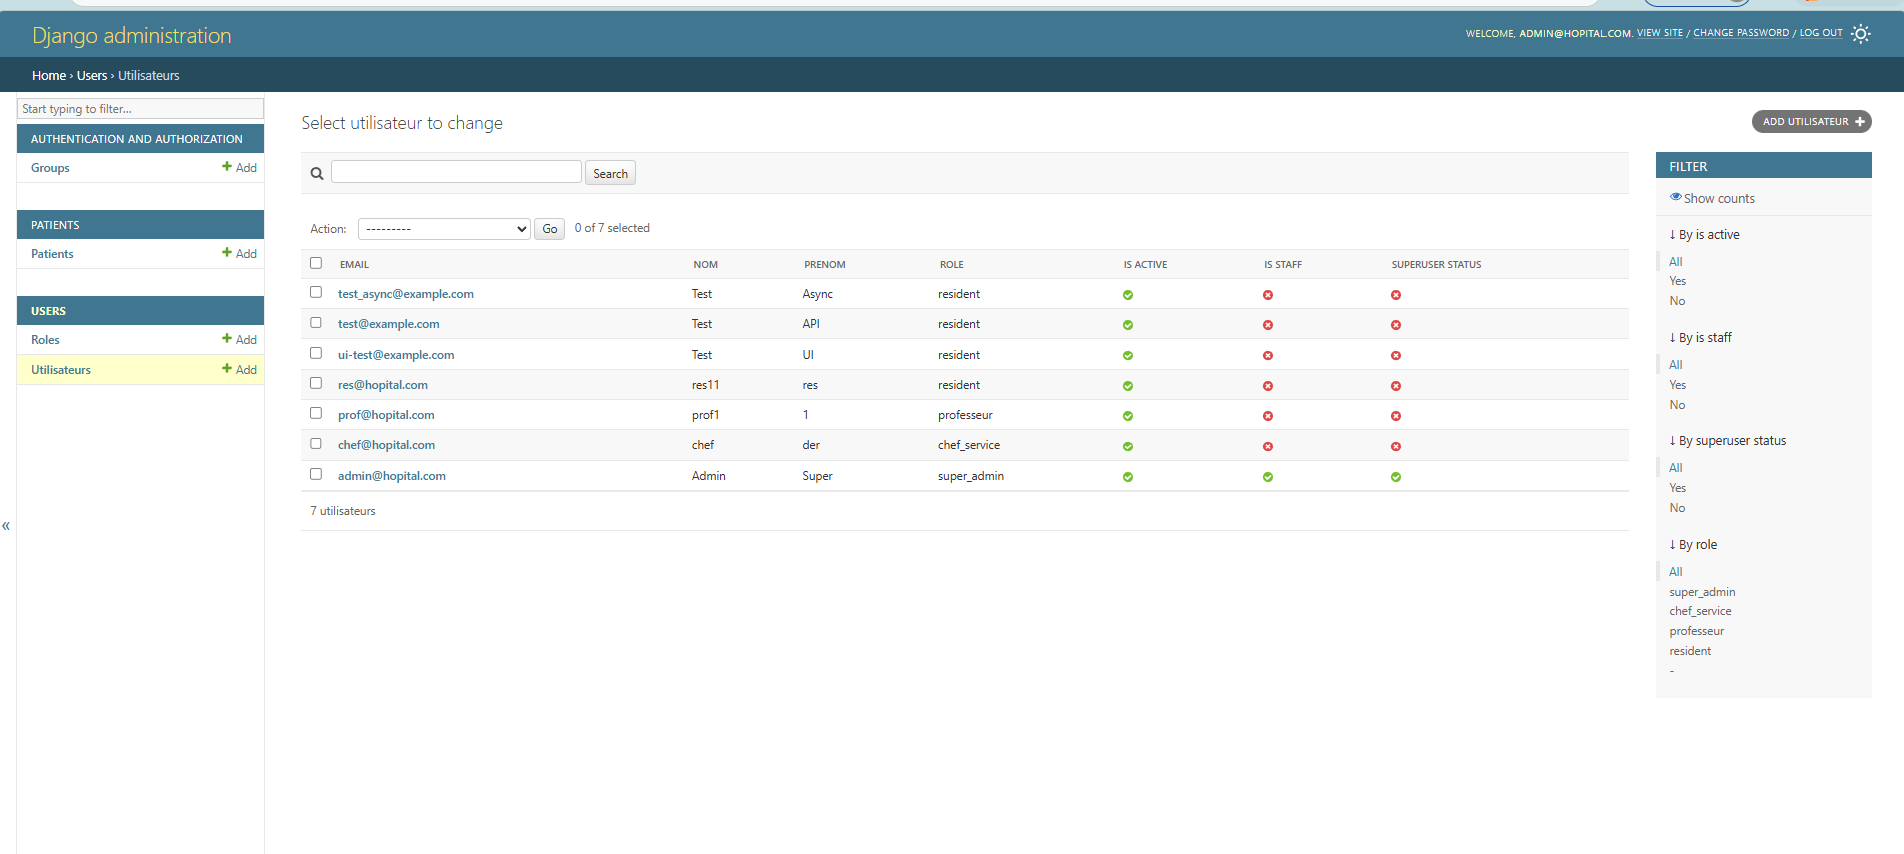
\includegraphics[width=0.88\textwidth]{screen/django.png}%
}{%
  \framebox[0.88\textwidth][c]{\rule{0pt}{5cm}\textit{django.png not found}}%
}
\caption{Django REST Framework --- modular application structure of the AI NéphroCare backend}
\label{fig:django_backend}
\end{figure}

%--- CLASS DIAGRAM ---
\subsection{Class Diagram}

Figure~\ref{fig:class_diagram} presents the UML class diagram of the five main Django models and their relationships, reflecting the static structure of the platform's PostgreSQL schema.

The \textbf{Role} model is intentionally minimal: it holds only the technical role name (\texttt{nom}), serving as the access-control reference table. It is linked to the \textbf{Utilisateur} model by a 1-to-many aggregation: one role can be assigned to many users, but each user has exactly one active role. The Utilisateur model stores user identity (unique email, full name, phone), hashed credentials, and exposes two methods: \texttt{login()} which issues a JWT token pair, and \texttt{change\_password()} which re-hashes the password.

The \textbf{Patient} model is the richest entity in the schema. It stores all clinical data as a flat collection of 160+ individual \texttt{TextField} columns, organized by clinical domain prefix (e.g., \texttt{demographie\_*}, \texttt{biologie\_*}, \texttt{dialyse\_*}). An additional \texttt{extra\_data} JSONField stores institution-specific dynamic columns. The \texttt{save()} method is overridden to auto-assign \texttt{id\_patient}. Feature extraction for the SVM model is handled by the external function \texttt{extract\_features\_for\_patient()} defined in \texttt{predictions/models/feature\_mapping.py}.

The \textbf{AuditLog} model records every sensitive action on the platform (create, update, delete, import, predict) with the entity identifier, a plain-text change description, the actor's IP address, and a precise timestamp. It is linked to Utilisateur by a 1-to-many association. The \textbf{PreprocessValidationRequest} model materializes the LLM preprocessing approval workflow: each session receives a unique \texttt{session\_id} (CharField, max 64 chars), a \texttt{status} field (\texttt{pending} / \texttt{approved} / \texttt{rejected}), and foreign keys to the submitting user (\texttt{submitted\_by\_id}) and reviewing user (\texttt{reviewed\_by\_id}).

\begin{figure}[htbp]
\centering
\resizebox{\textwidth}{!}{%
\begin{tikzpicture}[
  every node/.append style={outer sep=0pt},
  % title bar
  ctitle/.style={rectangle, draw=primary, line width=1.2pt, fill=primary,
                 text=white, font=\small\bfseries,
                 minimum width=5.0cm, minimum height=0.72cm,
                 align=center, inner sep=6pt},
  % attribute row
  cattr/.style={rectangle, draw=primary!35, line width=0.5pt,
                fill=white, text=navydark, font=\small,
                minimum width=5.0cm, minimum height=0.50cm,
                align=left, inner sep=5pt},
  % method row
  cmeth/.style={rectangle, draw=primary!35, line width=0.5pt,
                fill=primary!7, text=navydark, font=\small,
                minimum width=5.0cm, minimum height=0.50cm,
                align=left, inner sep=5pt},
  % wide variants (PreprocessValidationRequest)
  ctitleW/.style={ctitle, minimum width=5.8cm},
  cattrW/.style={cattr,   minimum width=5.8cm},
  % relationship arrows
  agg/.style={{Diamond[open,scale=1.4]}-{Stealth[scale=1.2]}, thick, draw=darkblue!75},
  assoc/.style={-{Stealth[scale=1.2]}, thick, draw=darkblue!65},
  rlbl/.style={font=\footnotesize\itshape, text=darkblue!85, fill=white, inner sep=1.5pt},
  card/.style={font=\footnotesize\bfseries, text=darkblue!90},
]

%━━━━━━━━━━━━━━━━━━━  ROW 1  ━━━━━━━━━━━━━━━━━━━━

%─── Role  @(0,0) ───
\node[ctitle] (r_t) at (0,0) {Role};
\node[cattr, below=0pt of r_t, anchor=north] (r1) {\underline{+ id : Integer (PK)}};
\node[cattr, below=0pt of r1,  anchor=north] (r2) {+ nom : CharField \textit{(unique)}};
\node[cattr, below=0pt of r2,  anchor=north] (r3) {Valeurs : super\_admin, chef\_service,};

%─── Utilisateur  @(7.5,0) ───
\node[ctitle] (u_t) at (7.5,0) {Utilisateur};
\node[cattr, below=0pt of u_t, anchor=north] (u1) {\underline{+ id : Integer (PK)}};
\node[cattr, below=0pt of u1,  anchor=north] (u2) {+ email : EmailField \textit{(unique)}};
\node[cattr, below=0pt of u2,  anchor=north] (u3) {+ nom, prenom : CharField};
\node[cattr, below=0pt of u3,  anchor=north] (u4) {+ telephone : CharField};
\node[cattr, below=0pt of u4,  anchor=north] (u5) {+ role\_id : FK $\to$ Role};
\node[cattr, below=0pt of u5,  anchor=north] (u6) {+ personal\_notes : TextField};
\node[cattr, below=0pt of u6,  anchor=north] (u7) {+ is\_active : Boolean};
\draw[primary!30, line width=0.8pt] (u7.south west) -- (u7.south east);
\node[cmeth, below=0pt of u7,  anchor=north] (um1) {+ login() : JWT};
\node[cmeth, below=0pt of um1, anchor=north] (um2) {+ change\_password()};

%─── Patient  @(15.5,0) ───
\node[ctitle] (p_t) at (15.5,0) {Patient};
\node[cattr, below=0pt of p_t, anchor=north] (p1) {\underline{+ id : Integer (PK)}};
\node[cattr, below=0pt of p1,  anchor=north] (p2) {+ id\_patient : CharField};
\node[cattr, below=0pt of p2,  anchor=north] (p3) {+ icc\_charlson : CharField};
\node[cattr, below=0pt of p3,  anchor=north] (p4) {+ demographie\_data : JSONB};
\node[cattr, below=0pt of p4,  anchor=north] (p5) {+ biologie\_data : JSONB};
\node[cattr, below=0pt of p5,  anchor=north] (p6) {+ dialyse\_data : JSONB};
\node[cattr, below=0pt of p6,  anchor=north] (p7) {+ \textit{[8 more JSONB sections]}};
\node[cattr, below=0pt of p7,  anchor=north] (p8) {+ extra\_data : JSONB};
\node[cattr, below=0pt of p8,  anchor=north] (p9) {+ utilisateur\_saisie : CharField};
\draw[primary!30, line width=0.8pt] (p9.south west) -- (p9.south east);
\node[cmeth, below=0pt of p9,  anchor=north] (pm1) {+ save()\ \ [auto-assign id\_patient]};
\node[cmeth, below=0pt of pm1, anchor=north] (pm2) {\textit{«predictions»}\ extract\_features\_for\_patient()};

%━━━━━━━━━━━━━━━━━━━  ROW 2 (y = -10)  ━━━━━━━━━━━━━━━━━━━━

%─── AuditLog  @(0,-10) ───
\node[ctitle] (a_t) at (0,-10) {AuditLog};
\node[cattr, below=0pt of a_t, anchor=north] (a1) {\underline{+ id : Integer (PK)}};
\node[cattr, below=0pt of a1,  anchor=north] (a2) {+ action : TextField};
\node[cattr, below=0pt of a2,  anchor=north] (a3) {+ entite, entite\_id};
\node[cattr, below=0pt of a3,  anchor=north] (a4) {+ details : TextField};
\node[cattr, below=0pt of a4,  anchor=north] (a5) {+ adresse\_ip : IPField};
\node[cattr, below=0pt of a5,  anchor=north] (a6) {+ date : DateTime};
\node[cattr, below=0pt of a6,  anchor=north] (a7) {+ utilisateur\_id : FK};

%─── PreprocessValidationRequest  @(8.2,-10) ───
\node[ctitleW] (pr_t) at (8.2,-10) {PreprocessValidationRequest};
\node[cattrW, below=0pt of pr_t, anchor=north] (pr1) {\underline{+ id : Integer (PK)}};
\node[cattrW, below=0pt of pr1,  anchor=north] (pr2) {+ session\_id : CharField(64)};
\node[cattrW, below=0pt of pr2,  anchor=north] (pr3) {+ source\_file\_name : CharField};
\node[cattrW, below=0pt of pr3,  anchor=north] (pr4) {+ status : CharField};
\node[cattrW, below=0pt of pr4,  anchor=north] (pr5) {+ submitted\_by\_id : FK};
\node[cattrW, below=0pt of pr5,  anchor=north] (pr6) {+ reviewed\_by\_id : FK};
\node[cattrW, below=0pt of pr6,  anchor=north] (pr7) {+ comment : TextField};

%━━━━━━━━━━━━━━━━━  RELATIONSHIPS  ━━━━━━━━━━━━━━━━━

% ① Role 1──◇──►* Utilisateur   (horizontal at title level, labels ABOVE)
\draw[agg]
  (r_t.east) --
    node[card, above, pos=0.06]{1}
    node[rlbl, above, pos=0.50]{has}
    node[card, above, pos=0.94]{*}
  (u_t.west);

% ② Utilisateur ──►* Patient   (CharField ref, not FK)
\draw[assoc]
  (u_t.east) --
    node[card, above, pos=0.06]{1}
    node[rlbl, above, pos=0.50]{saisie\_par (CharField)}
    node[card, above, pos=0.94]{*}
  (p_t.west);

% ③ Utilisateur 1──►1..* AuditLog
% Exit LEFT of Utilisateur bottom  →  LEFT in inter-row gap  →  DOWN into AuditLog
\draw[assoc]
  ($(u_t.south)+(-2.2,0)$)        % exit below-left of Utilisateur
  |-                               % horizontal then vertical
  (a_t.north)                      % arrive at AuditLog.north
  node[rlbl, right, pos=0.72]{1\,..\,* \ audit};

% ④ Utilisateur 1──►* PreprocessValidationRequest
% Exit RIGHT of Utilisateur bottom  →  DOWN  →  RIGHT into Preprocess
\draw[assoc]
  ($(u_t.south)+(2.0,0)$)         % exit below-right of Utilisateur
  -|                               % vertical then horizontal
  (pr_t.north)                     % arrive at Preprocess.north
  node[rlbl, right, pos=0.30]{submits};

\end{tikzpicture}%
}
\caption{UML Class Diagram --- main Django models}
\label{fig:class_diagram}
\end{figure}

\subsection{REST API Endpoints}

The platform exposes 45+ REST endpoints organized into four resource groups: \texttt{/api/auth/} for user management and authentication, \texttt{/api/patients/} for patient records and the import/preprocessing pipeline, \texttt{/api/predictions/} for SVM inference and model retraining, and \texttt{/api/audit/} for activity log consultation.

All endpoints follow standard REST conventions: HTTP verbs (\texttt{GET}, \texttt{POST}, \texttt{PATCH}, \texttt{DELETE}) express the operation intent, HTTP response codes (200, 201, 400, 401, 403, 404) explicitly indicate the outcome, and all responses are uniformly JSON. Every endpoint is protected by the DRF JWT middleware, which validates the access token before authorizing the request. Sensitive operations (deletion, model retraining, data integration) are further restricted by RBAC: only authorized roles can invoke them, with unauthorized attempts returning HTTP 403.

The \texttt{/api/patients/preprocess/} group implements a multi-step asynchronous workflow. A call to \texttt{analyze/} triggers a Celery task that submits the data to the Qwen2.5:14B LLM; the \texttt{status/} and \texttt{rows/} endpoints allow progress monitoring and display of proposed corrections; \texttt{cell-corrections/} allows a clinician to manually override an LLM suggestion; finally \texttt{integrate/} finalizes integration of the corrected data into the patient database after approval by the Head of Department or Super Admin.

Key endpoints are listed below:

\begin{longtable}{@{}
  >{\bfseries\footnotesize}p{1.3cm}
  >{\footnotesize\ttfamily\raggedright\arraybackslash}p{6.8cm}
  >{\footnotesize\raggedright\arraybackslash}p{5.5cm}@{}}
\caption{Principal REST API endpoints}\label{tab:api_endpoints}\\
\toprule
\textbf{Method} & \textbf{Endpoint} & \textbf{Description} \\
\midrule
\endfirsthead
\multicolumn{3}{c}{\tablename\ \thetable\ (continued)}\\
\toprule\textbf{Method} & \textbf{Endpoint} & \textbf{Description}\\\midrule
\endhead
\bottomrule
\endlastfoot
POST   & /api/auth/login/                           & JWT login $\rightarrow$ access + refresh token \\
POST   & /api/auth/token/refresh/                   & Refresh expired access token \\
GET    & /api/auth/utilisateurs/                    & List all users (admin) \\
POST   & /api/auth/utilisateurs/                    & Create user account \\
PATCH  & /api/auth/utilisateurs/\{id\}/             & Update user profile \\
DELETE & /api/auth/utilisateurs/\{id\}/             & Delete user (super admin) \\
GET    & /api/patients/                             & List patients (paginated, filterable) \\
POST   & /api/patients/                             & Create new patient record \\
GET    & /api/patients/\{id\}/                      & Full patient record \\
PATCH  & /api/patients/\{id\}/                      & Update patient data \\
POST   & /api/patients/import/                      & Import Excel/CSV file \\
GET    & /api/patients/export/                      & Export all patients as .xlsx \\
GET    & /api/patients/flat/                        & Flat view for analytics charts \\
POST   & /api/patients/preprocess/analyze/          & Start async LLM preprocessing \\
GET    & /api/patients/preprocess/\{sid\}/status/   & Preprocessing session status \\
GET    & /api/patients/preprocess/\{sid\}/rows/     & LLM-suggested corrections per row \\
GET    & /api/patients/preprocess/\{sid\}/\newline{}cell-corrections/   & Per-cell diff between original and corrected rows \\
POST   & /api/patients/preprocess/\{sid\}/\newline{}integrate/          & Finalize and integrate corrected data \\
POST   & /api/predictions/train/                    & Retrain SVM on current dataset \\
POST   & /api/predictions/predict-patient/          & Predict 1-year mortality for one patient \\
GET    & /api/predictions/metrics/                  & Model performance metrics \\
GET    & /api/audit/my-activity/                    & Last 10 actions of authenticated user \\
\end{longtable}

\section{Authentication \& Security}\label{sec:auth}

The platform implements stateless JWT-based authentication combined with role-based access control enforced at the API level.

\subsection{JWT Authentication}

AI NéphroCare uses \textbf{JSON Web Tokens (JWT)} via the \texttt{django\-restframe\-work\-simplejwt} library, following an OAuth2-compatible flow. Figure~\ref{fig:jwt_flow} illustrates the full exchange between the browser, the Django backend, and PostgreSQL.

\begin{figure}[htbp]
\centering
\resizebox{0.92\textwidth}{!}{%
\begin{tikzpicture}[
  actbox/.style={rectangle, draw=darkblue!80, fill=darkblue!72, text=white,
                 font=\small\bfseries, minimum width=3.2cm, minimum height=0.65cm,
                 align=center},
  lline/.style={dashed, gray!45, line width=0.9pt},
  fwd/.style={-{Stealth[scale=1.2]}, thick, darkblue!75},
  msglbl/.style={font=\scriptsize, fill=white, inner sep=1.5pt, midway, above, yshift=1pt},
  nnum/.style={font=\scriptsize\bfseries, text=primary, circle, draw=primary!60,
               inner sep=1.8pt, fill=white, line width=0.7pt},
  notebox/.style={draw=orange!55, fill=yellow!12, font=\scriptsize, inner sep=5pt,
                  align=left, rounded corners=3pt, text=navydark}
]
%--- Actors ---
\node[actbox] (C) at (0,0)    {Browser};
\node[actbox] (S) at (7.5,0)  {Django Backend};
\node[actbox] (D) at (14.5,0) {PostgreSQL};

%--- Lifelines ---
\draw[lline] (C.south) -- ++(0,-11);
\draw[lline] (S.south) -- ++(0,-11);
\draw[lline] (D.south) -- ++(0,-11);

%--- Step 1 : Login request ---
\node[nnum] at (-1.1,-1.2) {1};
\draw[fwd] (0,-1.2) -- node[msglbl]{POST /api/auth/login/} (7.5,-1.2);
\node[font=\scriptsize, text=textsec] at (3.75,-1.65) {body: \{email, password\}};

%--- Step 2 : DB verification ---
\node[nnum] at (-1.1,-2.5) {2};
\draw[fwd] (7.5,-2.5) -- node[msglbl]{SELECT user WHERE email=?} (14.5,-2.5);
\draw[fwd] (14.5,-3.2) -- node[msglbl]{bcrypt.verify() OK} (7.5,-3.2);

%--- Step 3 : Issue tokens ---
\node[nnum] at (-1.1,-4.1) {3};
\draw[fwd] (7.5,-4.1) -- node[msglbl]{access: JWT (8h),\ refresh: JWT (1d)} (0,-4.1);

%--- Payload note ---
\node[notebox] at (11.5,-5.2) {%
  \textbf{JWT Payload}\\
  user\_id, role, exp, iat\\
  Signature: HMAC-SHA256};

%--- Step 4 : Authenticated request ---
\node[nnum] at (-1.1,-6.3) {4};
\draw[fwd] (0,-6.3) -- node[msglbl]{GET /api/patients/ + Authorization: Bearer token} (7.5,-6.3);
\node[font=\scriptsize, text=textsec] at (5.5,-6.8) {verify HMAC-SHA256 signature};
\draw[fwd] (7.5,-7.5) -- node[msglbl]{200 OK + patient data} (0,-7.5);

%--- Step 5 : Token refresh ---
\node[nnum] at (-1.1,-8.5) {5};
\draw[fwd] (0,-8.5) -- node[msglbl]{POST /api/auth/token/refresh/ + refresh token} (7.5,-8.5);
\draw[fwd] (7.5,-9.2) -- node[msglbl]{new access JWT (8h)} (0,-9.2);
\node[font=\scriptsize, text=textsec, align=center] at (3.75,-9.8)
  {valid for 1 day; user must re-login after expiry};

\end{tikzpicture}}
\caption{JWT authentication flow: token issuance (Steps 1--3), authenticated request (Step~4), and token refresh using the refresh token (Step~5).}
\label{fig:jwt_flow}
\end{figure}

The detailed steps are as follows:
\begin{enumerate}
  \item The client sends \texttt{POST /api/auth/login/} with the user's email and password in JSON.
  \item The server validates the credentials against the hashed (bcrypt) password stored in the database.
  \item On success, the server returns a pair: \texttt{\{"access":\,"\allowbreak<jwt>",\,"refresh":\,"\allowbreak<jwt>"\}}.
  \item For every subsequent request the client attaches the header \texttt{Authorization:\allowbreak\ Bearer\ <token>}.
  \item When the access token expires (after \textbf{8 hours}), the client can call \texttt{POST /api/\allowbreak auth/\allowbreak token/\allowbreak refresh/} with the stored refresh token to obtain a new access token without re-entering credentials.
  \item The refresh token itself expires after \textbf{1 day}; after that the user must log in again.
\end{enumerate}

The JWT payload encodes: \texttt{user\_id}, \texttt{role} (string), \texttt{exp} (expiration Unix timestamp), and \texttt{iat} (issued-at timestamp). The server verifies the token signature using \textbf{HMAC-SHA256 (HS256)} with a 256-bit secret key stored in the environment variable \texttt{SECRET\_KEY}, which is never committed to version control.

\subsection{Role-Based Access Control (RBAC)}

The platform defines \textbf{four roles} with hierarchical permissions. Each HTTP request passes through a DRF permission class that extracts the role from the JWT payload and enforces the access policy.

\begin{table}[htbp]
\centering
\caption{RBAC permission matrix}\label{tab:rbac}
\begin{tabularx}{\textwidth}{lXp{3.5cm}}
\toprule
\textbf{Role} & \textbf{Permitted actions} & \textbf{Restricted from} \\
\midrule
\textbf{Admin} &
  Full access: user CRUD, patient management, preprocessing, predictions, audit log &
  — \\
\textbf{Head of Dept.} &
  Approve preprocessing sessions, view all patients, run predictions, read audit log &
  User CRUD, audit cleanup \\
\textbf{Resident} &
  Create and edit patients, submit preprocessing sessions for approval, run predictions &
  User management, audit log, preprocessing approval \\
\textbf{Professor} &
  Read-only access to patients and prediction results &
  All write operations \\
\bottomrule
\end{tabularx}
\end{table}

RBAC is enforced at two levels: (1) \textbf{Backend} — each DRF view carries a \texttt{permission\_classes} list that checks the role field from the JWT; (2) \textbf{Frontend} — the \texttt{ProtectedRoute} component reads the role from the \texttt{AuthContext} and redirects unauthorised users before the API call is even made.

\subsection{Additional Security Measures}

\begin{itemize}
  \item \textbf{Password hashing}: all passwords are stored using Django's \textbf{PBKDF2+SHA256} hasher (the framework default, enforced via \texttt{AUTH\_PASSWORD\_VALIDATORS}), which applies 870\,000 iterations making brute-force attacks computationally prohibitive. The \texttt{bcrypt} library is listed as a dependency for future migration to a bcrypt-based hasher in production.
  \item \textbf{Transport security}: the current deployment runs over HTTP on a local Docker network (\texttt{localhost:8000/3000}), which is acceptable for an intranet prototype. A production release would require TLS termination via a reverse proxy (e.g.\ Nginx + Let's Encrypt) and the Django settings \texttt{SECURE\_SSL\_REDIRECT}, \texttt{SESSION\_COOKIE\_SECURE}, and \texttt{CSRF\_COOKIE\_SECURE}. These hardening steps are identified as future work before any public-facing deployment.
  \item \textbf{CORS}: the \texttt{django-cors-headers} middleware restricts allowed origins to the declared frontend (\texttt{localhost:3000}), blocking cross-origin requests from any other domain.
  \item \textbf{Audit trail}: every state-changing action (create, update, delete on patients and users) is recorded in \texttt{AuditLog} with the actor's user ID, IP address, affected entity, and a text description of the change. The companion \texttt{HiddenAuditLog} table lets users hide individual log entries from their own view in the UI without deleting them from the database.
  \item \textbf{Input validation}: all incoming data passes through DRF serializers before reaching the model layer, enforcing field types, uniqueness constraints, and required/optional fields. Malformed requests are rejected with an HTTP 400 response identifying the offending field.
\end{itemize}

\section{API Design}\label{sec:api}

The REST API is built with Django REST Framework and organized around serializers, viewsets, and a structured URL namespace per application.

\subsection{DRF Serializers and Validation}

Django REST Framework \textbf{serializers} sit between the HTTP layer and the database layer. Every endpoint uses a dedicated serializer that validates field types and constraints (e.g.\ \texttt{EmailField} uniqueness, required vs.\ optional fields), handles nested representations (e.g.\ the patient serializer structures the different data sections into a consistent response), and enforces write-protection on computed fields such as \texttt{date\_creation} and \texttt{utilisateur\_saisie}.

Validation errors return HTTP \textbf{400 Bad Request} with a structured JSON body where each key is the offending field name and the value is a list of error messages. For example, submitting a duplicate email returns \texttt{\{"email": ["This field must be unique."]\}}.

\subsection{Filtering and Search}

The patient list endpoint (\texttt{GET /api/patients/}) returns a JSON object containing a \texttt{results} array and a \texttt{count} field. Filtering is implemented directly in the view layer via query parameters: \texttt{?search=} performs a full-text search across patient name, ID, and medical fields; \texttt{?sexe=}, \texttt{?age\_min=}, \texttt{?age\_max=}, \texttt{?statut\_inclusion=}, and \texttt{?date\_naissance=} allow targeted field-level filtering. All parameters can be combined freely in a single request.

\subsection{Prediction Response Structure}

The \texttt{POST /api/predictions/predict-patient/} endpoint assembles the patient's clinical features, runs them through the calibrated SVM pipeline, and returns a structured JSON response designed to be directly usable by clinicians:

\begin{itemize}
  \item \texttt{risk\_level} — categorical classification: \textit{Low} ($<$10\,\%), \textit{Moderate} (10–29\,\%), or \textit{High} ($\geq$29\,\%)
  \item \texttt{score} — mortality risk expressed as a percentage (0–100)
  \item \texttt{probability} — Platt-scaled probability of 1-year mortality (0–1), output of \texttt{CalibratedClassifierCV}
  \item \texttt{factors} — ordered list of the most influential clinical features with their SVM weight and direction
  \item \texttt{recommendation} — auto-generated clinical text summarising the risk level and key factors
  \item \texttt{features\_used} — list of feature keys actually used in the prediction
  \item \texttt{n\_features} — count of non-missing features used
  \item \texttt{model} — identifier of the SVM model file used, enabling audit reproducibility
  \item \texttt{doietal\_risk\_score} / \texttt{doietal\_risk\_category} — secondary risk score based on the Doi et al.\ clinical index
\end{itemize}

\section{Frontend Architecture}\label{sec:frontend}

The frontend is a single-page React application organized around context-based state management, protected routing, and a centralized Axios HTTP client.

\subsection{React Structure}

The React application is organized around:
\begin{itemize}
  \item \textbf{Context API}: \texttt{AuthContext} (JWT state, login/logout)
  \item \textbf{Protected Routes}: \texttt{ProtectedRoute} component enforces RBAC at the routing level
  \item \textbf{Axios Instance}: Centralized HTTP client with JWT interceptor and error handling
\end{itemize}

\subsection{Pages and Interfaces}

\begin{description}

  \item[\textbf{Landing Page} (\texttt{/})] The landing page is the public entry point of the platform, accessible without authentication. It presents the platform identity through a full-screen hero layout composed of a gradient background in deep blue tones, a large anatomical illustration of kidneys on the right side, and a concise value proposition on the left: the platform name \textit{AI NéphroCare}, the tagline \textit{"Welcome to your health space"}, a short description inviting users to open their secure account, and a \textbf{"Get started"} call-to-action button that redirects to the login page.

\begin{figure}[htbp]
\centering
\IfFileExists{landing_page.png}{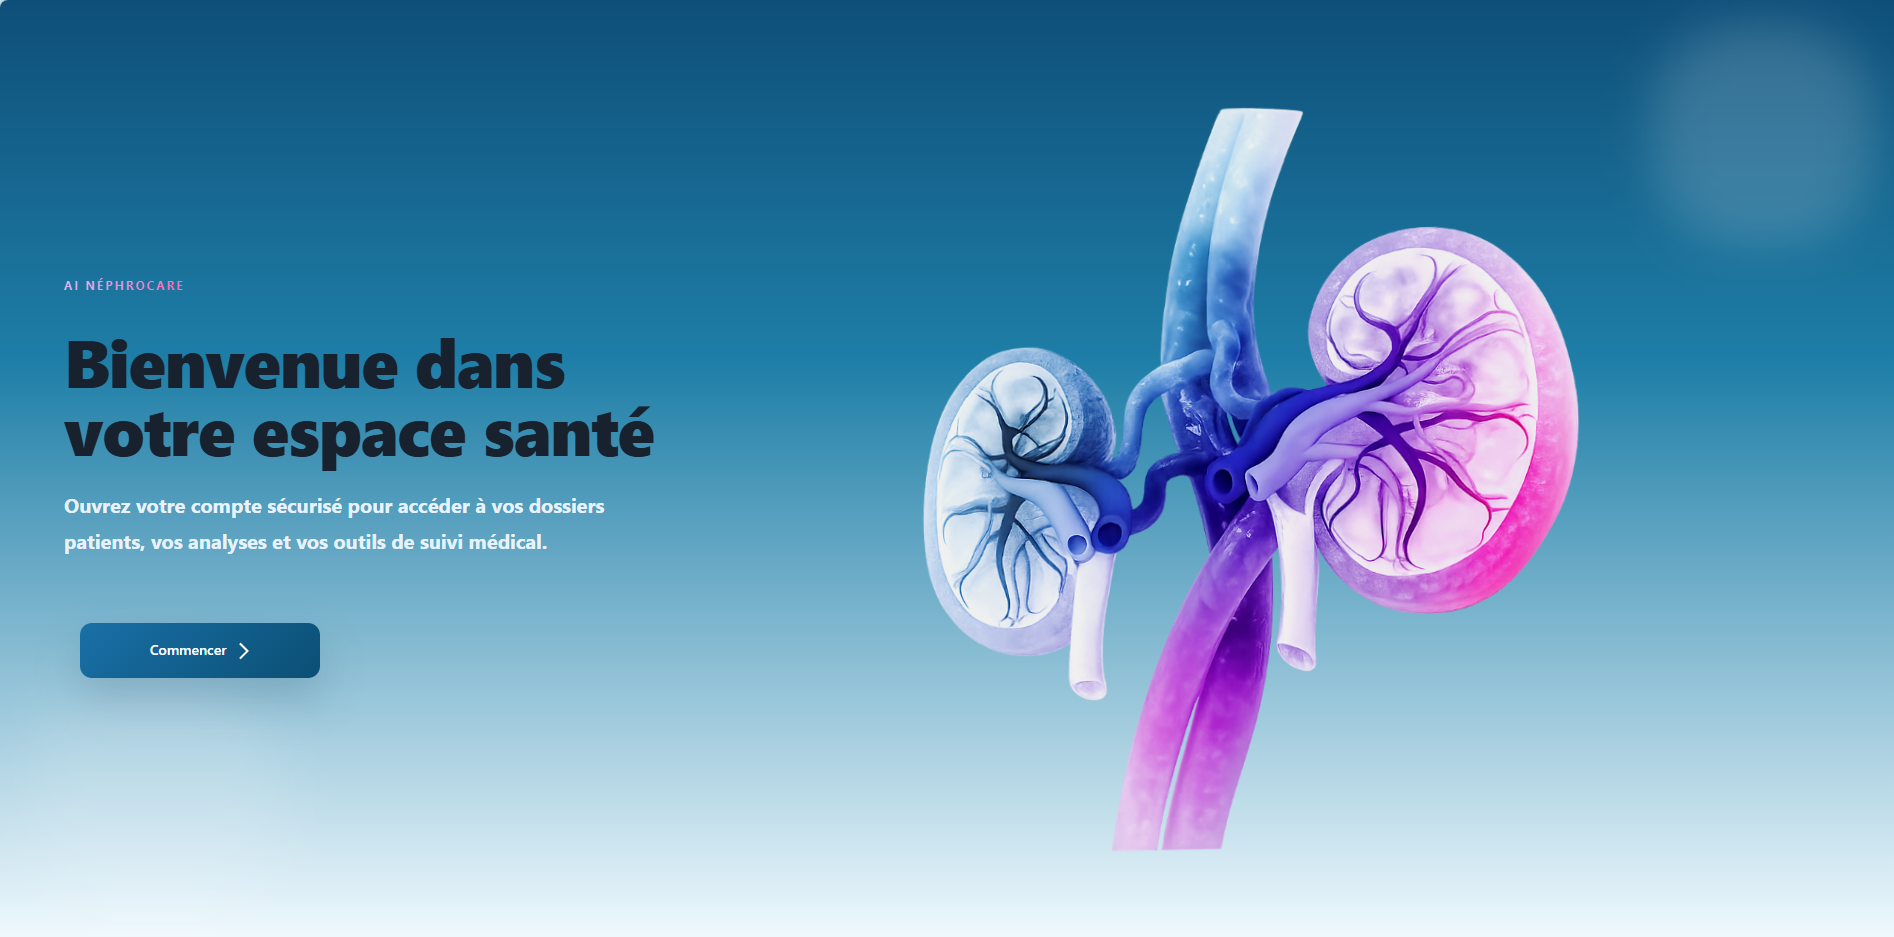
\includegraphics[width=0.85\textwidth]{landing_page.png}}{\framebox[0.85\textwidth][c]{\small[Screenshot: Landing Page]}}
\caption{Landing page --- public entry point of the AI NéphroCare platform}
\label{fig:landing}
\end{figure}

  \item[\textbf{Login Page} (\texttt{/login})] The login page is divided into two panels. The left panel displays the platform branding: the name \textit{AI NéphroCare} in large pink typography over a dark blue background, accompanied by a 3D kidney illustration and the subtitle \textit{"Une plateforme intelligente dédiée à la néphrologie, pensée pour vos patients et vos équipes."}. The right panel presents a minimal authentication form over a white background with floating decorative dots, containing:
\begin{itemize}
  \item An \textbf{email} input field with envelope icon
  \item A \textbf{password} input field with padlock icon
  \item A \textbf{Connexion} submit button that initiates the JWT authentication flow (POST \texttt{/api/auth/login/})
\end{itemize}
On successful authentication, the user is redirected to their role-appropriate dashboard. On failure, an error message is displayed inline without page reload.

\begin{figure}[htbp]
\centering
\IfFileExists{login_page.png}{
\includegraphics[width=0.85\textwidth]{login_page.png}}{\framebox[0.85\textwidth][c]{\small[Screenshot: Login Page]}}
\caption{Login page --- split-panel design with branding (left) and JWT authentication form (right)}
\label{fig:login}
\end{figure}

  \item[\textbf{Navigation Sidebar}] Once authenticated, all pages share a persistent left sidebar (width: 248 px) that serves as the main navigation hub of the application. It is composed of:
\begin{itemize}
  \item \textbf{Platform logo and branding} at the top (\textit{AI NÉPHROCARE}), with a gradient gradient typography
  \item \textbf{Navigation card} with links to all main sections: Dashboard, Patients, Analyse IA, Monitor
  \item \textbf{User profile card} at the bottom showing the connected user's email and role badge
  \item \textbf{Notifications button} (visible to Head of Department and Super Admin only) with a badge counter for pending validation requests
  \item \textbf{Logout button} that clears the JWT tokens and redirects to the login page
\end{itemize}

Access to each section is controlled by the user's role (RBAC): navigation items are filtered at the routing level via the \texttt{ProtectedRoute} component, so unauthorised sections are never rendered.

\begin{figure}[htbp]
\centering
\IfFileExists{sidebar.png}{
\includegraphics[width=0.3\textwidth]{sidebar.png}}{\framebox[0.3\textwidth][c]{\small[Screenshot: Navigation Sidebar]}}
\caption{AI NéphroCare navigation sidebar --- persistent across all authenticated pages}
\label{fig:sidebar}
\end{figure}

\paragraph{Digital Notepad (global floating notepad).}
All authenticated pages include a \textbf{floating action button} (bottom-right corner) that opens a persistent personal notepad called \textit{Digital Notepad}. The notepad allows clinicians to write private reminders, observations, or annotations that are auto-saved at regular intervals and stored in their user profile (\texttt{personal\_notes} field). The panel displays the last save time and offers a \textbf{Clear} button to erase the content.

\begin{figure}[htbp]
\centering
\IfFileExists{carnet.png}{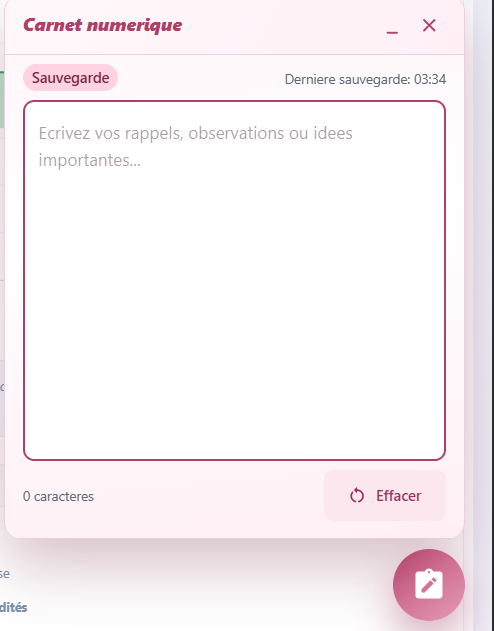
\includegraphics[width=0.40\textwidth]{carnet.png}}{\framebox[0.40\textwidth][c]{\small[Screenshot: Digital Notepad floating notepad]}}
\caption{Digital Notepad --- persistent personal notepad accessible from any authenticated page via a floating action button}
\label{fig:carnet}
\end{figure}

  \item[\textbf{Dashboard} (\texttt{/dashboard})] The dashboard is the first authenticated page. Its content is entirely \textbf{role-dependent}: Super Admin and Head of Department see an administrative dashboard focused on user governance, while Professor and Resident see a clinical dashboard focused on their own activity.

% ──────────────────────────────────────────────────────────────────────────────
\subsubsection*{Dashboard --- Super Admin and Head of Department}
% ──────────────────────────────────────────────────────────────────────────────

The administrative dashboard is organised into two columns:
\begin{itemize}
  \item \textbf{Left column} — Connected profile card (identity, role, email, telephone).
  \item \textbf{Right column} — User management area: KPI summary, user list with search, and CRUD panel.
\end{itemize}

\paragraph{KPI summary.}
The hero banner displays \textbf{7 interactive KPI cards} for Super Admin (6 for Head of Department, excluding Super Admins):
\textit{Active}, \textit{Inactive}, \textit{Super Admins}, \textit{Heads of Dept.}, \textit{Professors}, \textit{Residents}, \textit{Roles}.
Each card is \textbf{clickable}: clicking it filters the \textit{Managed Accounts} list below to show only matching accounts (by status or role). An active filter is displayed as a labelled chip with a dismiss button. The text search bar operates \textbf{in parallel} with the KPI filter.

\begin{figure}[htbp]
\centering
\IfFileExists{dashboard_kpi.png}{
\includegraphics[width=0.85\textwidth]{dashboard_kpi.png}}{\framebox[0.85\textwidth][c]{\small[Screenshot: Admin dashboard --- KPI cards]}}
\caption{Super Admin dashboard --- 7 interactive KPI cards in the hero banner; clicking a card filters the account list}
\label{fig:dashboard_kpi}
\end{figure}

\begin{figure}[htbp]
\centering
\IfFileExists{dashboard_filter.png}{
\includegraphics[width=0.85\textwidth]{dashboard_filter.png}}{\framebox[0.85\textwidth][c]{\small[Screenshot: KPI filter active]}}
\caption{KPI filter active --- clicking \textit{Professors} restricts the list and displays an active-filter chip}
\label{fig:dashboard_filter}
\end{figure}

\paragraph{User Management (CRUD).}
Clicking the \textit{Afficher} toggle reveals the CRUD panel. The form supports:
\begin{itemize}
  \item \textbf{Create}: email, telephone, last name, first name, role, status, initial password (no confirmation password required).
  \item \textbf{Edit}: pencil icon pre-fills the form; administrator must re-enter their \textbf{own password} before saving (\texttt{confirmation\_password} validated server-side via \texttt{check\_password()}).
  \item \textbf{Delete}: bin icon opens a dialog requiring the administrator's password before deletion.
\end{itemize}

\begin{figure}[htbp]
\centering
\IfFileExists{dashboard_crud.png}{
\includegraphics[width=0.85\textwidth]{dashboard_crud.png}}{\framebox[0.85\textwidth][c]{\small[Screenshot: CRUD form]}}
\caption{User management CRUD panel --- account creation and editing form}
\label{fig:dashboard_crud}
\end{figure}

\begin{figure}[htbp]
\centering
\IfFileExists{dashboard_delete_confirm.png}{
\includegraphics[width=0.70\textwidth]{dashboard_delete_confirm.png}}{\framebox[0.70\textwidth][c]{\small[Screenshot: Delete confirmation dialog]}}
\caption{Deletion confirmation dialog --- password required before account removal}
\label{fig:dashboard_delete_confirm}
\end{figure}

The \textbf{double-authentication} on write operations prevents unauthorised modifications and ensures every change is traceable in the audit log.

\paragraph{Import validation workflow.}
When a Resident or Professor submits a preprocessed file for approval, the Head of Department receives a \textbf{notification badge} in the sidebar. Clicking \textbf{"Preview"} opens a preview modal showing file name, submitter, row/column counts, quality score, and the first 15 rows. From the modal, the Head of Department can \textbf{validate and integrate} (data inserted into the patient database) or close without action. A reject action is available via the detail endpoint with a mandatory reason.

\begin{figure}[htbp]
\centering
\IfFileExists{demande_soumission.png}{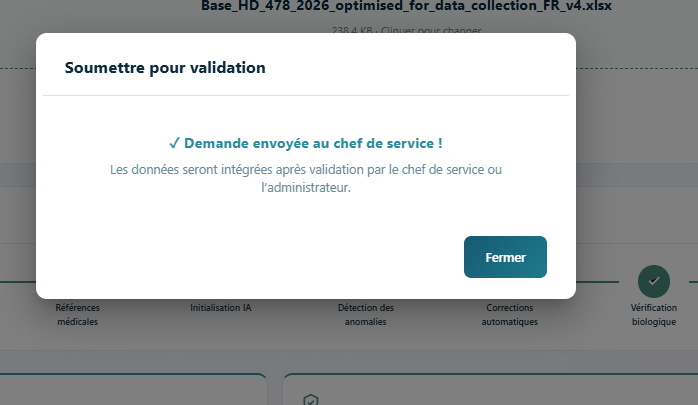
\includegraphics[width=0.85\textwidth]{demande_soumission.png}}{\framebox[0.85\textwidth][c]{\small[Screenshot: Import submission request view]}}
\caption{Import submission request --- clinician view showing file pending review with status indicator}
\label{fig:demande_soumission}
\end{figure}

\begin{figure}[htbp]
\centering
\IfFileExists{apercu_validation.png}{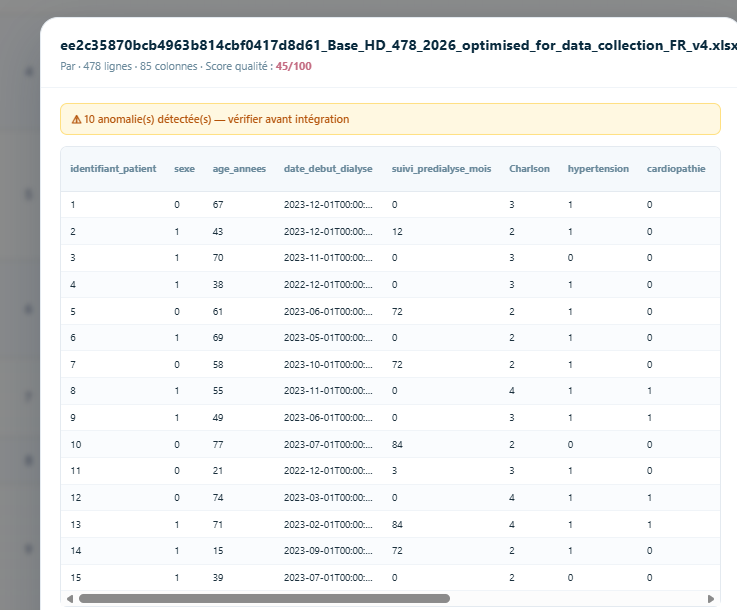
\includegraphics[width=0.85\textwidth]{apercu_validation.png}}{\framebox[0.85\textwidth][c]{\small[Screenshot: Head of Department validation preview modal]}}
\caption{Import validation preview --- Head of Department reviews file metadata, row/column count, quality score and first rows before approving or rejecting}
\label{fig:apercu_validation}
\end{figure}

% ──────────────────────────────────────────────────────────────────────────────
\subsubsection*{Dashboard --- Professor and Resident}
% ──────────────────────────────────────────────────────────────────────────────

Clinical users (Professor, Resident) see a dedicated dashboard with \textbf{no administrative panels}. The layout presents two side-by-side panels:

\begin{itemize}
  \item \textbf{Left panel} — Connected profile card: avatar with initials, full name, role badge, email, telephone.
  \item \textbf{Right panel} — \textbf{Recent Activity}: a real-time feed of the last 10 actions performed by the connected user, fetched from \texttt{GET /api/audit/my-activity/}. Each entry shows a colour-coded indicator, a human-readable label, and a timestamp. The entries tracked include:
  \begin{itemize}
    \item Patient added, modified, or deleted
    \item Mortality prediction launched
    \item Preprocessing file submitted for validation
    \item Import approved or rejected by the chef
  \end{itemize}
\end{itemize}

\begin{figure}[htbp]
\centering
\IfFileExists{dashboard_resident.png}{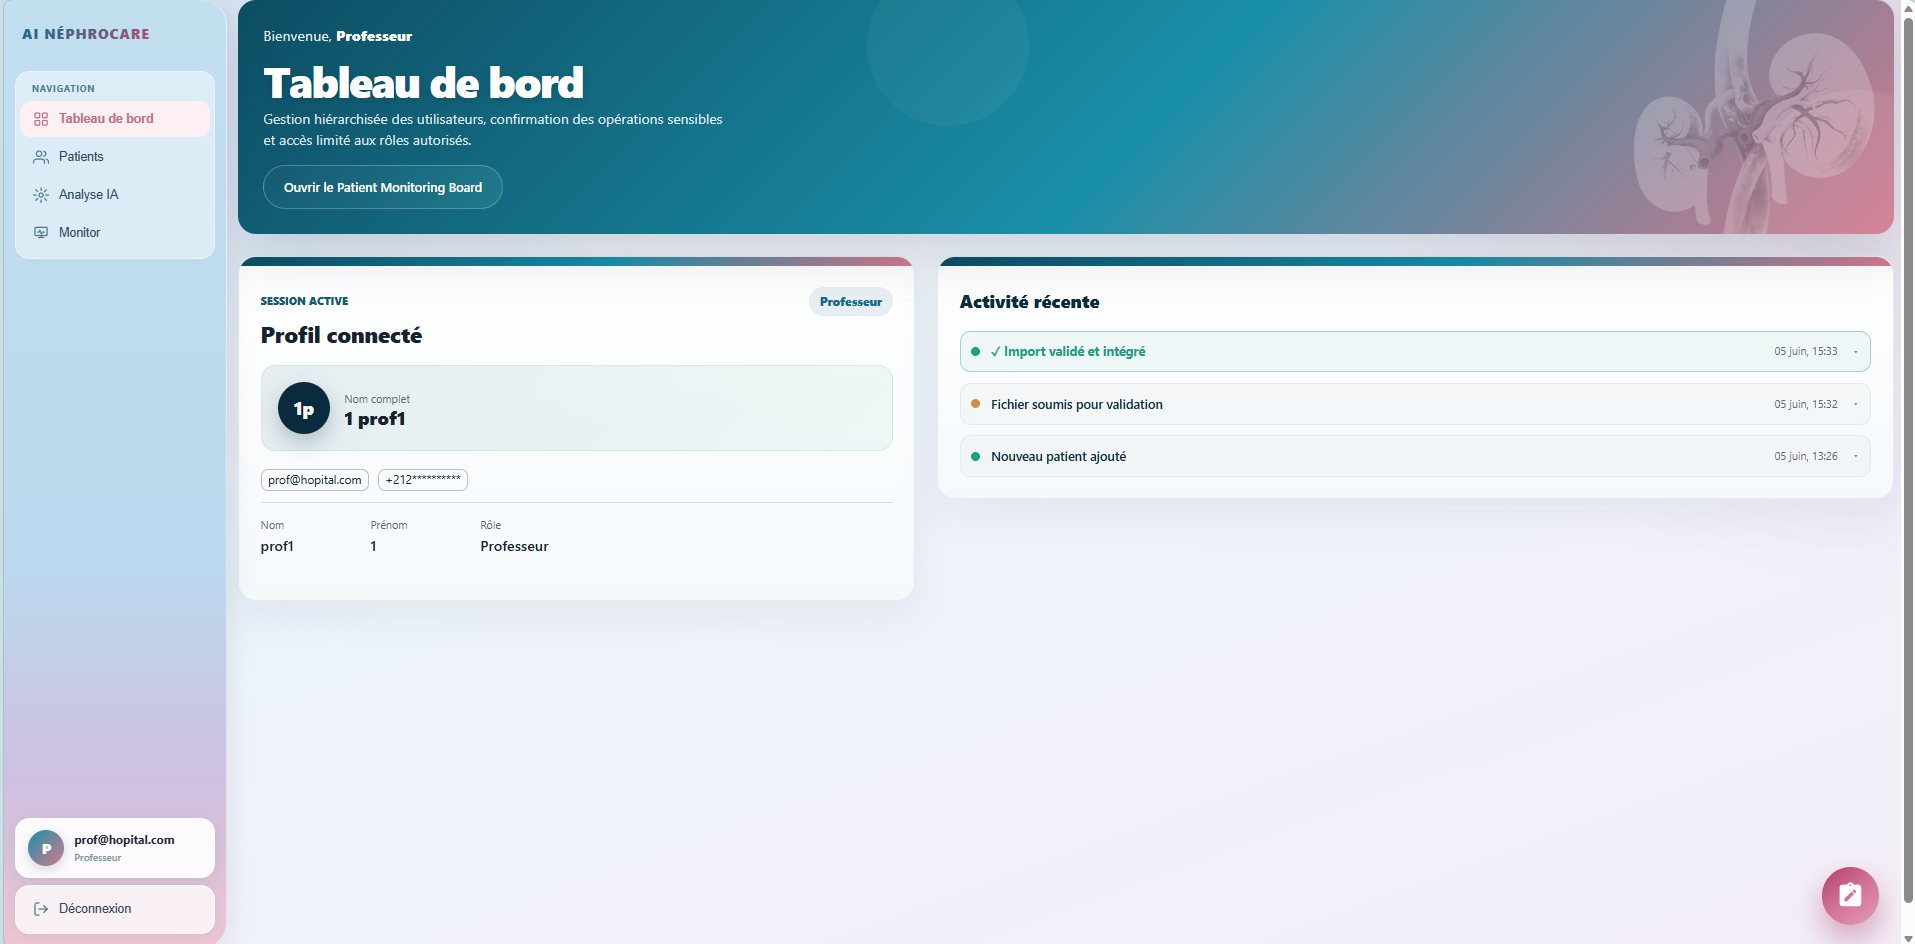
\includegraphics[width=0.85\textwidth]{dashboard_resident.png}}{\framebox[0.85\textwidth][c]{\small[Screenshot: Professor/Resident dashboard --- profile + activity feed]}}
\caption{Professor/Resident dashboard --- connected profile (left) and recent activity feed (right)}
\label{fig:dashboard_resident}
\end{figure}

\paragraph{Click-to-expand interaction.}
Clicking any activity entry \textbf{expands} it inline to reveal: the full action detail (e.g.\ patient identifier), any comment left by the reviewer, the entity reference, and a \textit{"View →"} shortcut to the relevant section (patient list, AI model, or preprocessing tab). Clicking again collapses the entry.

\begin{figure}[htbp]
\centering
\IfFileExists{dashboard_activity_expand.png}{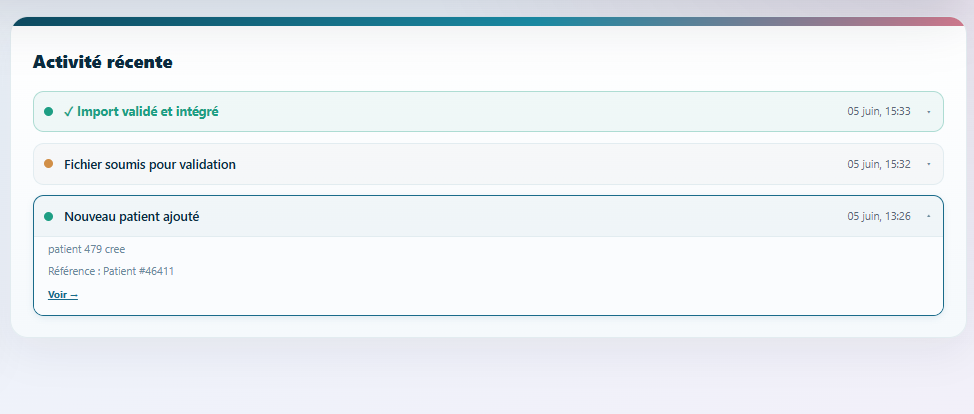
\includegraphics[width=0.75\textwidth]{dashboard_activity_expand.png}}{\framebox[0.75\textwidth][c]{\small[Screenshot: Activity entry expanded --- full detail, comment, entity reference, navigation link]}}
\caption{Activity feed entry expanded --- full action detail, reviewer comment, and direct navigation shortcut}
\label{fig:dashboard_activity_expand}
\end{figure}

\paragraph{Import decision notifications.}
When the Head of Department or Super Admin approves or rejects a submitted import, the backend writes an \texttt{AuditLog} entry in the \textbf{submitter's} log. The entry appears with a \textbf{distinct visual style}:
\begin{itemize}
  \item \textbf{Approved}: green border and bold label \textit{"\checkmark{} Import validated and integrated"} with the reviewer's name and comment.
  \item \textbf{Rejected}: pink border and bold label \textit{"$\times$ Import rejected"} with the rejection reason.
\end{itemize}
This ensures the clinician is immediately informed of the outcome of their submission without requiring a separate notification system.

\begin{figure}[htbp]
\centering
\IfFileExists{dashboard_notif_decision.png}{
\includegraphics[width=0.75\textwidth]{dashboard_notif_decision.png}}{\framebox[0.75\textwidth][c]{\small[Screenshot: Import decision notification --- approved (green) or rejected (pink)]}}
\caption{Import decision notification in the activity feed --- green entry for approval, pink entry for rejection, both displaying the reviewer's comment}
\label{fig:dashboard_notif_decision}
\end{figure}

  \item[\textbf{Patient Management} (\texttt{/patients})] The patient management module is organized into three tabs presented in the following logical order: \textit{Preprocessing}, \textit{Data Management}, and \textit{Analysis}.

\subsubsection*{Tab 1 --- Preprocessing Interface}

The preprocessing tab is the entry point for data quality control. It guides the user through a four-step workflow: file upload, AI analysis, correction review, and integration. The platform uses the \textbf{Qwen2.5:14B} large language model deployed locally via \textbf{Ollama}, chosen for its strong reasoning on structured clinical tabular data, its on-premises deployment (patient data never leaves the hospital network), and its 14B parameters that allow contextualised corrections with medical justification.

\begin{figure}[htbp]
\centering
\IfFileExists{preproc_overview.png}{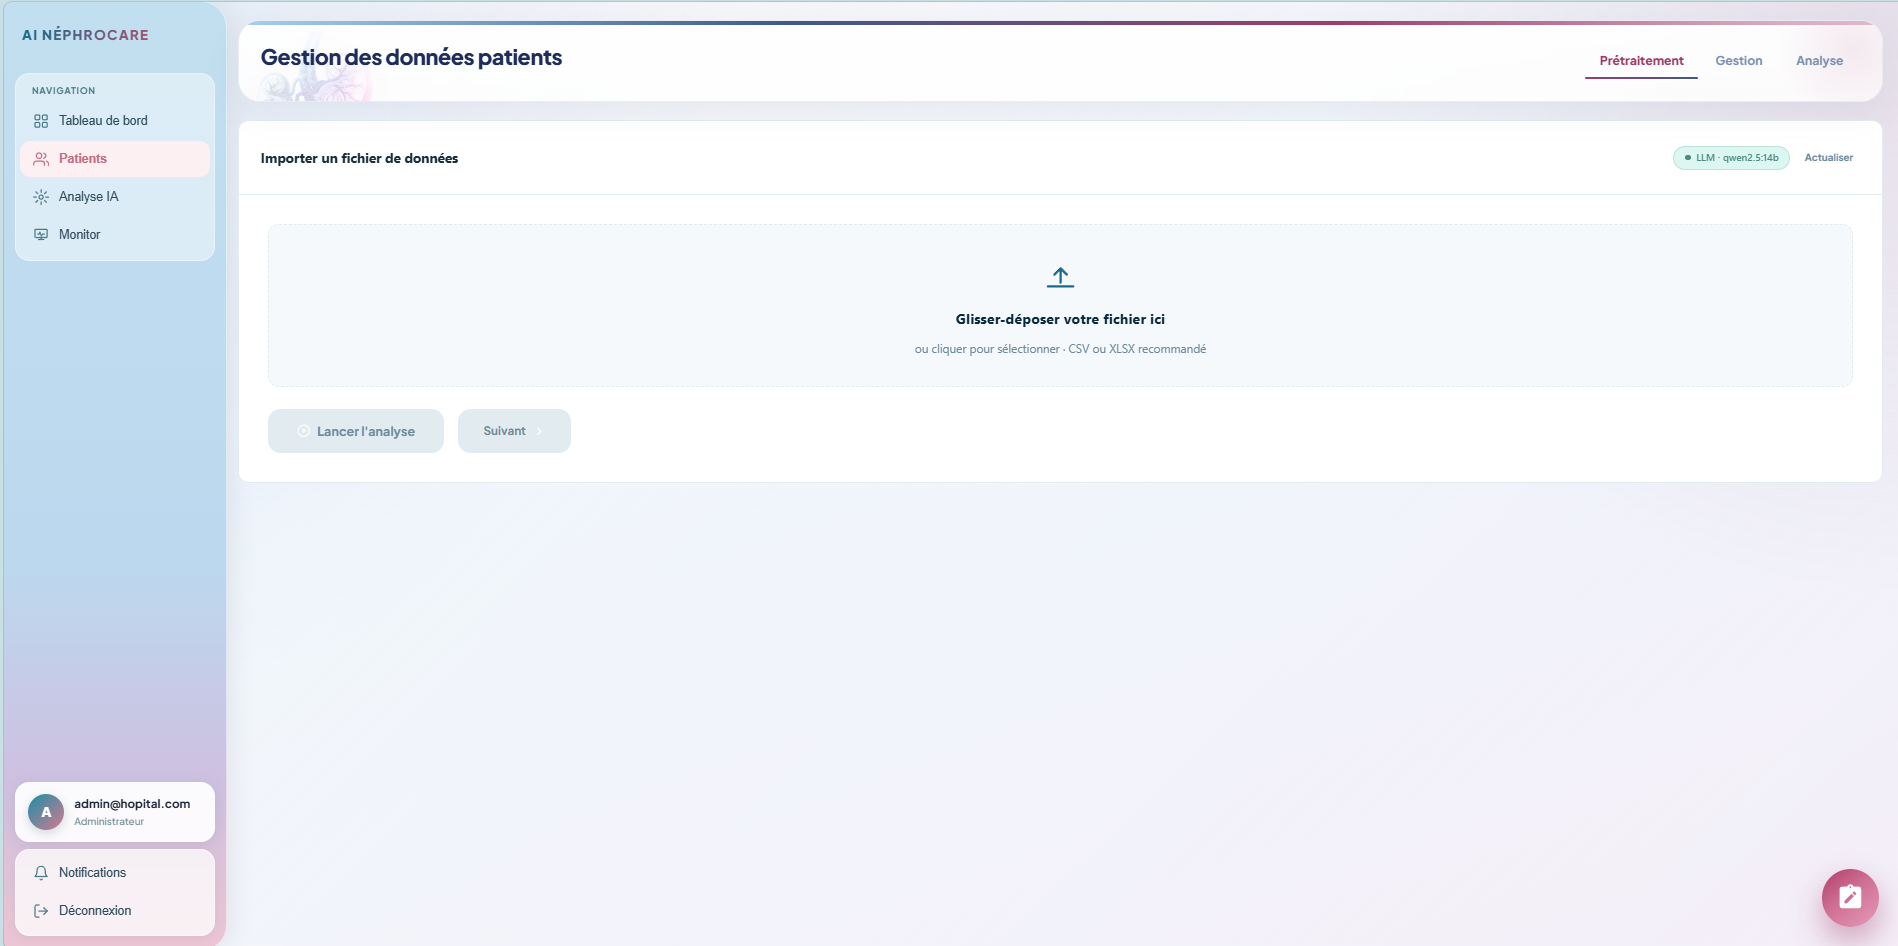
\includegraphics[width=0.85\textwidth]{preproc_overview.png}}{\framebox[0.85\textwidth][c]{\small[Screenshot: Preprocessing interface --- general view]}}
\caption{Preprocessing interface --- general view before file upload}
\label{fig:preproc_overview}
\end{figure}

\paragraph{Step 1 — File upload.}
The interface presents a \textbf{drag-and-drop upload zone} that accepts \texttt{.xlsx} and \texttt{.csv} files. Upon file selection, the platform validates the format, displays the file name, and enables the analysis launch button.

\begin{figure}[htbp]
\centering
\IfFileExists{preproc_upload.png}{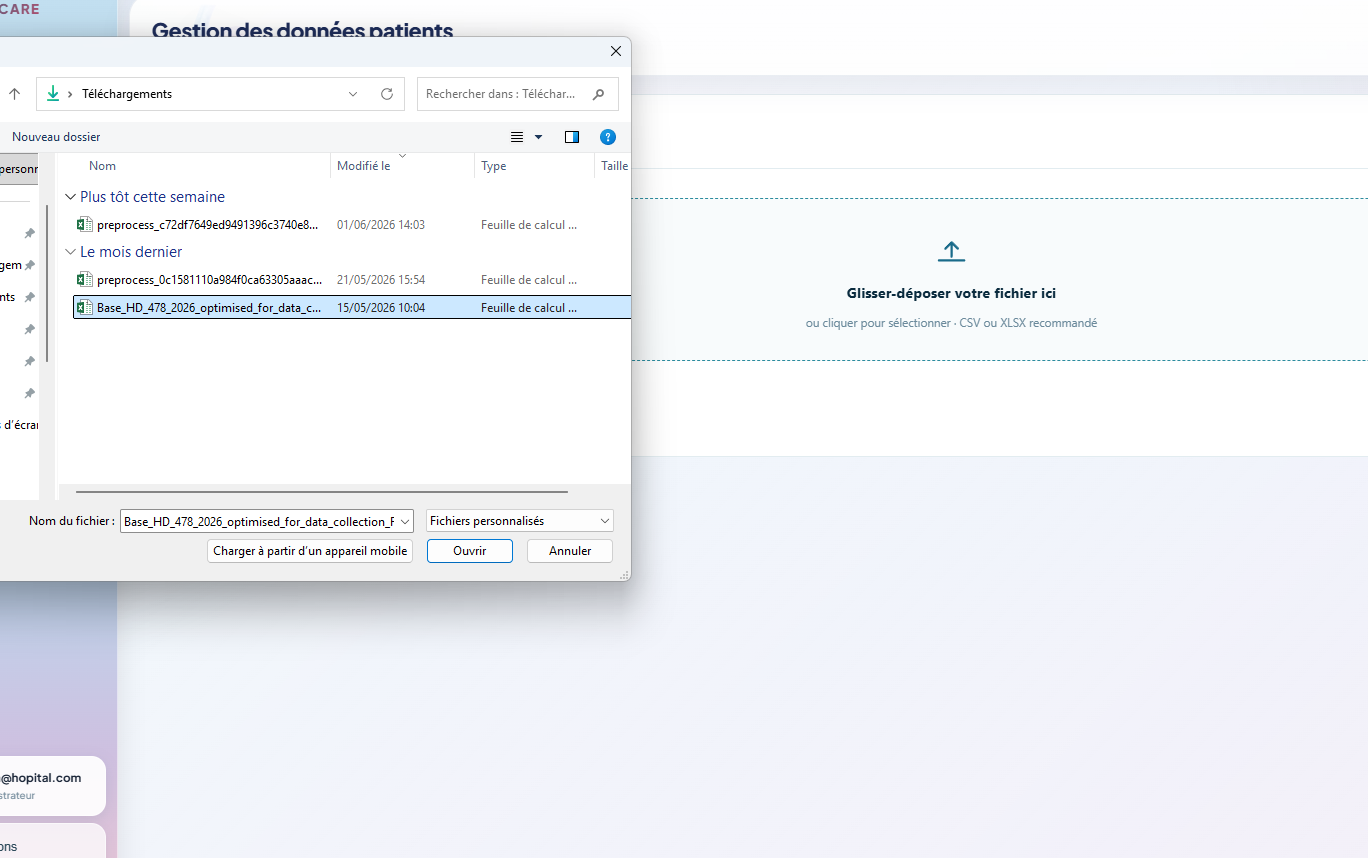
\includegraphics[width=0.85\textwidth]{preproc_upload.png}}{\framebox[0.85\textwidth][c]{\small[Screenshot: File upload --- Excel/CSV file selected]}}
\caption{Step 1 --- file upload zone with Excel/CSV file selected, ready for LLM analysis}
\label{fig:preproc_upload}
\end{figure}

\paragraph{Step 2 — Analysis pipeline (11 stages).}
Clicking \textbf{"Run LLM Analysis"} triggers an asynchronous \textbf{Celery} task (\texttt{analyze\_preprocess\_async}) that orchestrates the following eleven-stage pipeline. Each stage updates the progress bar and status message visible on the frontend.

Table~\ref{tab:pipeline_stages} maps each backend stage to the label displayed in the interface progress bar.

\begin{table}[htbp]
\centering
\caption{Preprocessing pipeline stages and corresponding interface labels}
\label{tab:pipeline_stages}
\footnotesize\begin{tabularx}{\textwidth}{cp{5.2cm}p{3cm}X}
\toprule
\textbf{\#} & \textbf{Backend function} & \textbf{Role} & \textbf{Interface label} \\
\midrule
1  & \texttt{\_read\_uploaded\_dataframe}         & File parsing         & File reading \\
2  & \texttt{\_build\_technical\_profile}         & Statistical scan     & Data analysis \\
3  & \texttt{\_build\_preprocess\_chunks}         & RAG chunking         & Preparation \\
4  & \texttt{\_build\_retrieval\_context}         & ChromaDB retrieval   & Medical references \\
5  & \texttt{\_determine\_preprocess\_route}      & LLM routing          & AI initialization \\
6  & \texttt{\_call\_ollama\_qwen\_analysis}      & LLM batch analysis   & Anomaly detection \\
7  & \texttt{\_apply\_llm\_correction\_plan}      & Apply corrections    & Automatic corrections \\
8  & \texttt{\_run\_bio\_value\-\_correction\_pass} & LOINC/KB bio pass  & Biological verification \\
9  & \texttt{\_run\_llm\_flagged\_corrections}    & Flagged value triage & Clinical verification \\
10 & \texttt{\_run\_model\_imputation}            & KNN imputation       & Data completion \\
11 & \texttt{\_build\_preprocess\_report}         & Quality report       & Final report \\
\bottomrule
\end{tabularx}
\end{table}

\begin{enumerate}

  \item \textbf{File reading.} The uploaded Excel or CSV file is parsed into a Pandas DataFrame. All column names and data types are preserved as-is from the source file.

  \item \textbf{Technical profiling.} Python performs a full statistical scan of \textbf{every column}: data types, missing value rates, unique value counts, outlier detection, and anomaly candidate identification (sentinel values, biologically impossible values, Excel artefacts, future dates). This stage produces a \texttt{technical\_profile} dictionary used to ground all subsequent stages without any LLM call.

  \item \textbf{Semantic chunking for RAG.} The dataset is split into semantic row-chunks by clinical domain (11 sections: demography, IRC, comorbidities, biology, dialysis, complications, etc.), capping at 40 rows per chunk while preserving patient coherence. These chunks are not sent to the LLM; they serve exclusively as retrieval units for ChromaDB.

  \item \textbf{RAG retrieval.} The chunks are used to query ChromaDB, which stores embeddings of nephrology clinical guidelines, LOINC reference ranges, and dialysis protocol summaries. The top-$k$ most relevant document fragments are injected into the LLM prompt as medical grounding context.

  \item \textbf{Route determination.} The platform evaluates dataset complexity and selects the analysis mode: \textit{LLM-only} (default), \textit{deterministic} (Python rules only, no LLM), or \textit{hybrid}. In the deployed configuration the route is always LLM with \texttt{qwen2.5:14b} as primary model.

  \item \textbf{LLM batch analysis — Pass 1.} All columns are split into batches of 5 (\texttt{LLM\_BATCH\_SIZE=5}). For each batch, all row values of the 5 columns are serialised and sent to Qwen2.5:14B with the RAG context. The model returns a structured \texttt{correction\_plan} (JSON) specifying type casts, date parsing, missing value fills, and flagged anomalies. Results from all batches are merged into a single correction plan. For a 90-column dataset this produces at most $\lceil 90/5 \rceil = 18$ LLM calls.

  \item \textbf{Apply correction plan.} The merged \texttt{correction\_plan} is applied to the full DataFrame: numeric type casts, date standardisation, boolean normalisation, fill-missing values, and Excel artefact removal.

  \item \textbf{Biological value correction pass.} For each column matched to a LOINC code (primary) or the medical knowledge base (fallback), the platform asks the LLM to identify aberrant unique values based on authoritative clinical reference ranges, then corrects them across all rows.

  \item \textbf{LLM flagged corrections.} Columns flagged in Pass 1 but not covered by the bio KB are re-analysed. Each suspicious value is classified as \textit{error} (auto-corrected), \textit{extreme\_real} (extreme but clinically plausible --- kept with flag), or \textit{uncertain} (kept with flag). Only confirmed errors are automatically corrected.

  \item \textbf{KNN imputation.} Values nullified by the correction passes are re-estimated using K-Nearest Neighbours ($k=5$), inferring each missing value from the 5 most similar patients across all available clinical features.

  \item \textbf{Report generation.} A final quality report is assembled: quality score (0--100), total corrections, column-level issues, LLM confidence contract, and pipeline metadata. The session is persisted and the frontend is notified that the analysis is complete.

\end{enumerate}

\subsubsection*{Python Deterministic Pre-passes}

In addition to the LLM passes, the \texttt{\_apply\_llm\_correction\_plan()} function runs a set of \textbf{deterministic Python pre-passes} before the LLM correction plan is applied. These handle unambiguous error patterns that do not require LLM interpretation:

\begin{itemize}
  \item \textbf{Excel serial-date artefacts}: values such as \texttt{1899-12-30} or \texttt{1900-01-01} (produced by pandas when reading Excel serial date~0) are unconditionally replaced with \texttt{null}.

  \item \textbf{\texttt{"X"} values in numeric columns}: in columns where at least 60\% of non-null values are numeric, any cell containing \texttt{"X"}, \texttt{"x"}, or \texttt{"*"} is replaced with \texttt{null} and subsequently imputed by KNN. Text/categorical columns are left untouched.

  \item \textbf{Mixed semicolon artefacts}: values of the form \texttt{1;(1/2024)} are detected by a dedicated regex and flagged for the LLM to classify and correct.

  \item \textbf{Decimal comma normalisation}: French-locale numbers such as \texttt{1,5} or \texttt{2~234,56} in object columns are converted to their dot-decimal equivalents (\texttt{1.5}, \texttt{2234.56}).
\end{itemize}

These pre-passes ensure that obvious structural errors are removed \textit{before} the LLM analysis, reducing noise in the LLM prompt and preventing trivially incorrect values from being classified as \textit{uncertain}.

The interface displays a \textbf{progress view} (MUI \texttt{LinearProgress}) updated after each stage, with a status message tracking the current step and a \textbf{cancel button} to interrupt the Celery task at any point. The frontend polls \texttt{GET /api/patients/preprocess/\{session\_id\}/status/} every 3 seconds via a \texttt{setInterval} hook.

\begin{figure}[htbp]
\centering
\IfFileExists{preproc_progress.png}{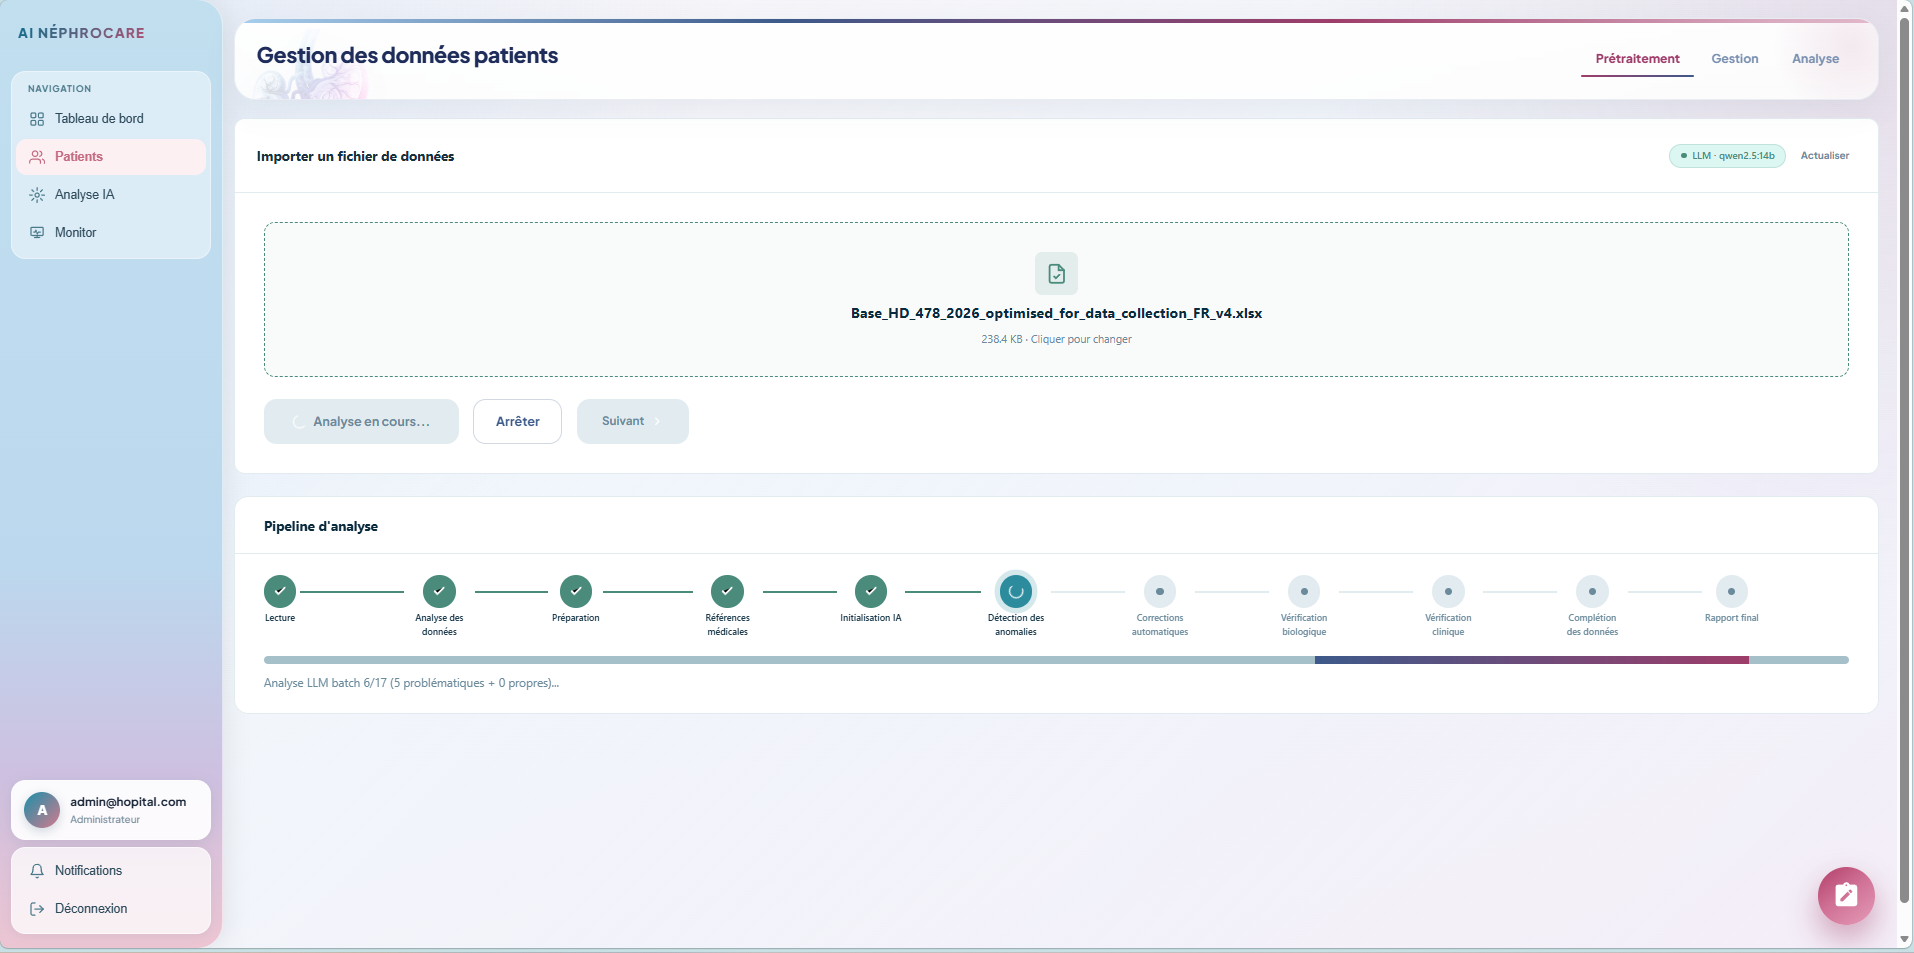
\includegraphics[width=0.85\textwidth]{preproc_progress.png}}{\framebox[0.85\textwidth][c]{\small[Screenshot: Analysis in progress --- LinearProgress bar and status message]}}
\caption{Step 2 --- LLM analysis in progress, real-time progress bar with current processing message}
\label{fig:preproc_progress}
\end{figure}

\paragraph{Step 3 --- LLM correction review table.}
Once the analysis completes, the interface displays a \textbf{results summary} followed by the \textbf{correction review table}. The summary section contains:

\begin{itemize}
  \item A \textbf{Quality Score ring} (custom SVG \texttt{ScoreRing} component, range 0--100): green if $\geq 80$, orange if $\geq 50$, red below 50
  \item Three \textbf{KPI stat cards} (custom \texttt{StatCard} component, MUI \texttt{Paper}):
    \begin{itemize}
      \item \textbf{Rows analysed} — total number of rows processed by the LLM
      \item \textbf{Cells corrected} — number of individual cell values automatically corrected
      \item \textbf{Suspicious columns} — number of columns flagged as anomalous but without an automatic correction (manual review recommended)
    \end{itemize}
\end{itemize}

The correction review table is organised in two \textbf{tabs} (MUI \texttt{Tabs} / \texttt{Tab}):

\begin{enumerate}
  \item \textbf{Corrected cells} — lists every automatic correction with the following columns:
    \begin{itemize}
      \item \textbf{Row} — row index in the source file
      \item \textbf{Patient ID} — patient identifier
      \item \textbf{Column} — clinical field name
      \item \textbf{Original value} — raw value from the imported file
      \item \textbf{Corrected value} — value proposed by the LLM (clickable: the user can \textbf{edit it inline} to override the suggestion)
      \item \textbf{Type} — correction category (type cast, outlier, KNN imputation, boolean normalisation, Excel artefact)
      \item \textbf{Justification} — medical explanation generated by Qwen2.5:14B
    \end{itemize}
    Each corrected cell is rendered as a \textbf{MUI \texttt{Chip}} colour-coded by correction type (green for corrected, pink for KNN). Clicking a cell activates an \textbf{inline text field} to manually override the LLM's suggestion; the override is persisted via \texttt{POST /api/patients/preprocess/\{session\}/apply-overrides/}.

  \item \textbf{Suspicious columns} — lists columns flagged by the LLM as potentially erroneous but for which no automatic correction was applied. Each row shows the column name, anomaly category, and LLM justification so the user can decide on a manual correction.
\end{enumerate}

Below the table, two \textbf{export buttons} allow the user to download the data as an \texttt{.xlsx} file before integration:

\begin{itemize}
  \item \textbf{Export corrected (.xlsx)} — downloads the corrected version. The file is generated server-side by the \texttt{PatientPreprocessExportView} using the \texttt{openpyxl} library and contains \textbf{two sheets}:
    \begin{itemize}
      \item \textbf{Sheet 1 — ``Data''}: the full dataset with all corrections applied. Every cell whose value was changed by the LLM is \textbf{highlighted in pale yellow} (\texttt{\#FFF2CC}) with a \textbf{bold orange font} (\texttt{\#B45309}), making modified cells immediately visible. The header row uses a dark navy background (\texttt{\#0A2B3E}) with white bold text.
      \item \textbf{Sheet 2 — ``Corrections''}: a summary table listing every changed cell with the columns \textit{Row no.}, \textit{Patient ID}, \textit{Column}, \textit{Original value}, \textit{Corrected value}, \textit{Type}, and \textit{Justification} — identical structure to the on-screen review table.
    \end{itemize}
  \item \textbf{Export original (.xlsx)} — downloads the raw file as imported, with only the header row styled, and no cell highlighting.
\end{itemize}

\begin{figure}[htbp]
\centering
\IfFileExists{preproc_export_donnees.png}{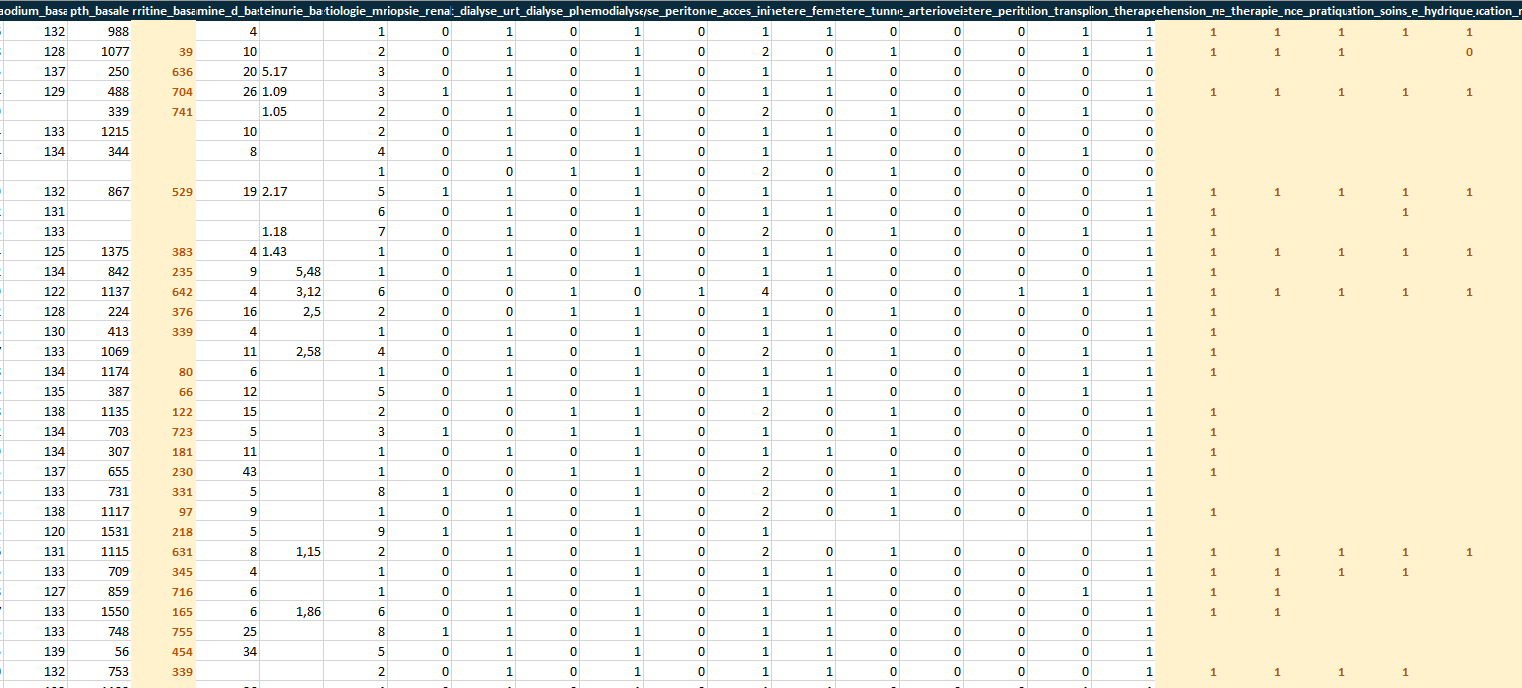
\includegraphics[width=0.85\textwidth]{preproc_export_donnees.png}}{\framebox[0.85\textwidth][c]{\small[Screenshot: ``Data'' sheet --- LLM-modified cells highlighted in yellow]}}
\caption{\textit{Data} sheet of the exported \texttt{.xlsx} file --- cells modified by the LLM are highlighted in pale yellow (\texttt{\#FFF2CC}) with bold orange font, generated by \texttt{openpyxl}}
\label{fig:preproc_export_donnees}
\end{figure}

\begin{figure}[htbp]
\centering
\IfFileExists{preproc_export_corrections.png}{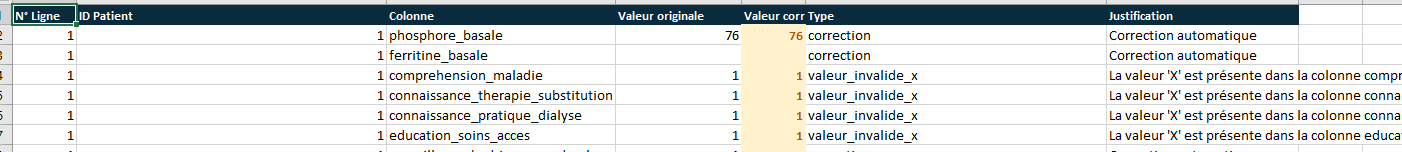
\includegraphics[width=0.85\textwidth]{preproc_export_corrections.png}}{\framebox[0.85\textwidth][c]{\small[Screenshot: ``Corrections'' sheet --- summary table of all modifications]}}
\caption{\textit{Corrections} sheet of the exported \texttt{.xlsx} file --- summary table listing each modified cell with its original value, corrected value, correction type, and medical justification}
\label{fig:preproc_export_corrections}
\end{figure}

\begin{figure}[htbp]
\centering
\IfFileExists{preproc_corrections.png}{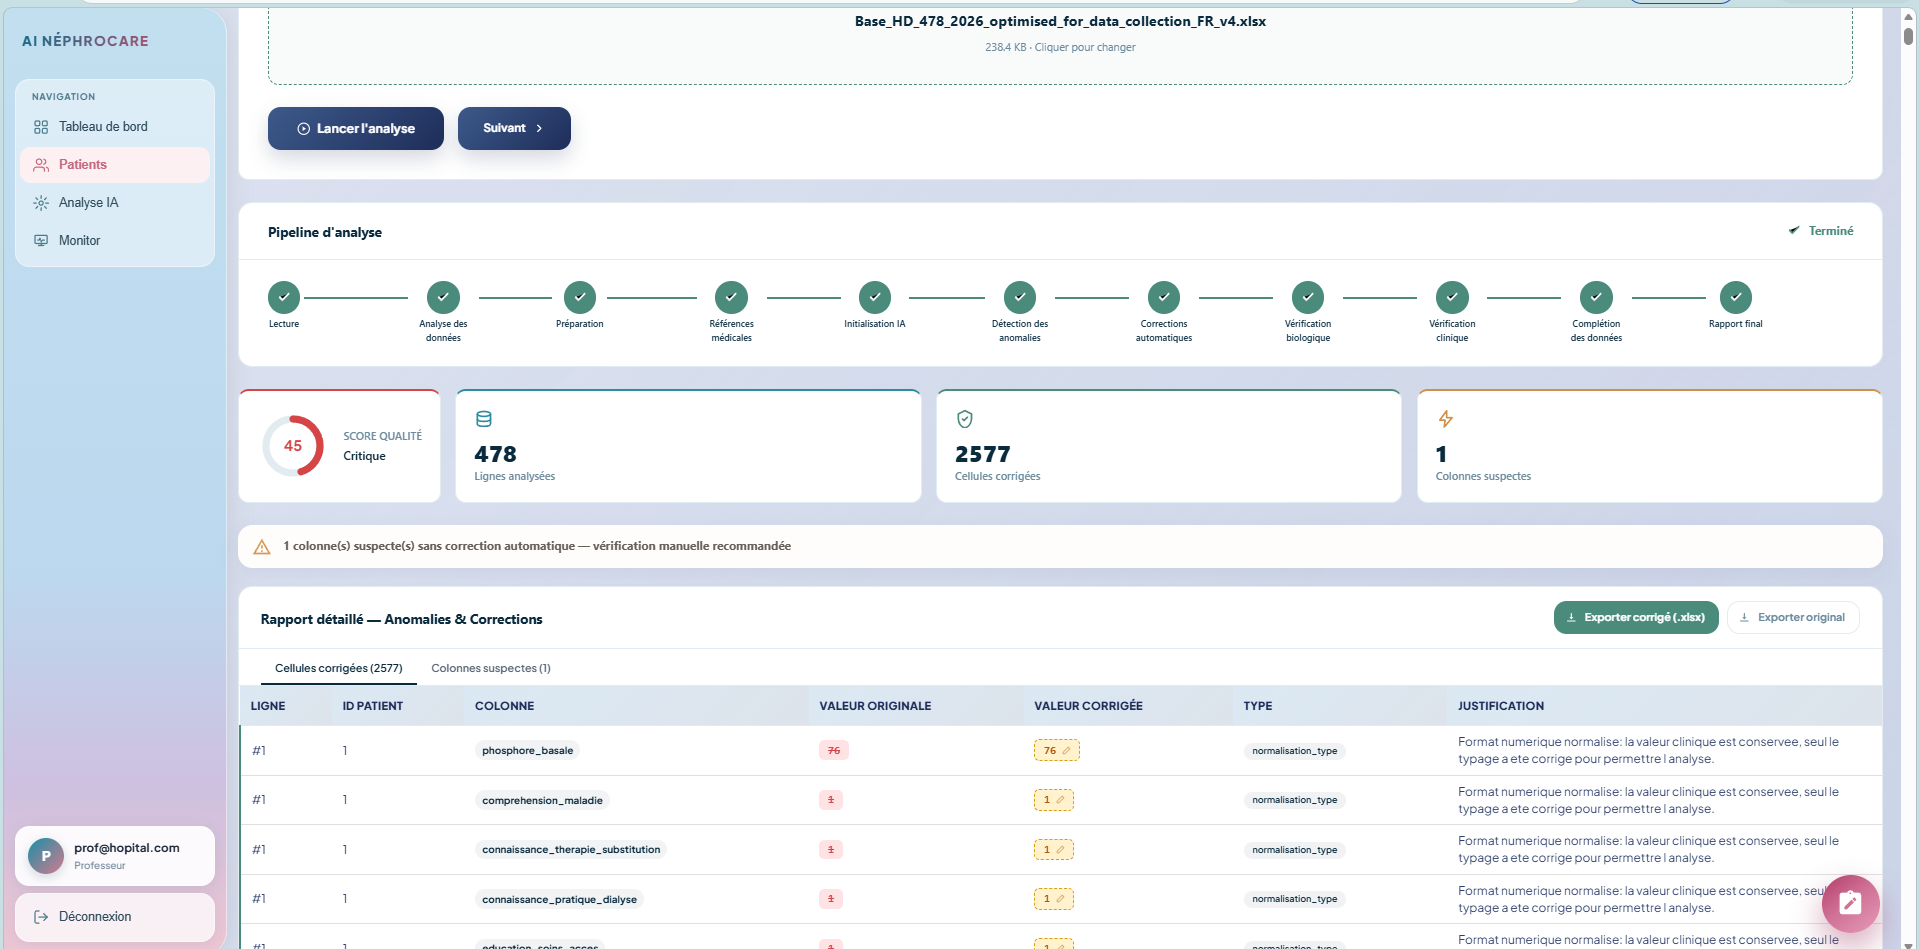
\includegraphics[width=0.85\textwidth]{preproc_corrections.png}}{\framebox[0.85\textwidth][c]{\small[Screenshot: LLM correction review table]}}
\caption{Step 3 --- LLM correction review table: quality score, KPI cards, and cell-level corrections with medical justifications}
\label{fig:preproc_corrections}
\end{figure}

\paragraph{Step 4 --- Integration.}
Once the user has reviewed and optionally overridden corrections, they click \textbf{"Integrate into platform"} to persist the dataset into the platform database. Before confirming, the user must explicitly \textbf{choose which version to integrate} via a radio-button selector:

\begin{itemize}
  \item \textbf{Corrected version} (recommended) --- the dataset with all LLM corrections, bio-value corrections, and KNN imputation applied. This is the version that will improve the downstream SVM prediction accuracy.
  \item \textbf{Original version} --- the raw file as uploaded, without any modifications. This option is available if the clinician considers the original data reliable and does not wish to apply the automated corrections.
\end{itemize}

This explicit choice guarantees that no data modification reaches the database without the user's deliberate consent, in line with the platform's principle of \textbf{human-in-the-loop} clinical validation.

\begin{figure}[htbp]
\centering
\IfFileExists{preproc_integration_choice.png}{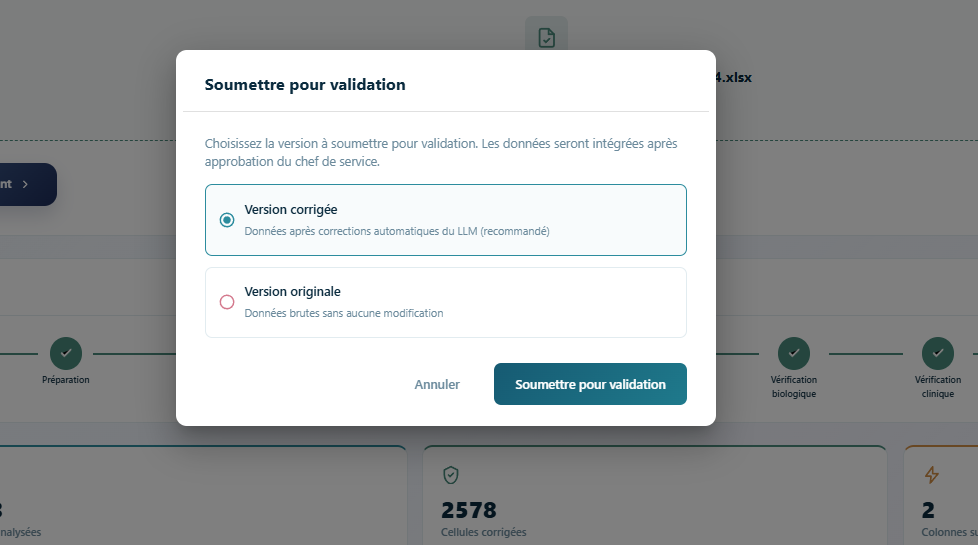
\includegraphics[width=0.75\textwidth]{preproc_integration_choice.png}}{\framebox[0.75\textwidth][c]{\small[Screenshot: Version selector --- corrected vs original]}}
\caption{Integration version selector --- the user chooses between the corrected version (recommended) and the original file before persisting data to the database}
\label{fig:preproc_integration_choice}
\end{figure}

Once the version is selected and confirmed, the integration endpoint triggers a \textbf{column mapping process} that translates the source file's column names into the platform's standardised schema:

\begin{itemize}
  \item Each source column is compared against a configurable mapping dictionary (\texttt{column\_mapping.json}). If a match is found (e.g.\ \textit{"Albumine basale"} $\rightarrow$ \texttt{albumine\_basale}), the value is stored in the corresponding field of the patient's structured clinical record.
  \item Columns that belong to a known clinical section (demography, biology, dialysis, comorbidities, etc.) are stored in the relevant JSONB section of the \texttt{Patient} model.
  \item Columns that do \textbf{not} match any predefined field are stored as \textbf{dynamic columns} in the \texttt{extra\_data} JSONB field, preserving institution-specific variables without requiring any schema migration.
\end{itemize}

A success notification confirms the integration, and the system transitions automatically to the \textbf{Data Management tab} where the imported patients are immediately visible.

\subsubsection*{Tab 2 --- Data Management}

\begin{figure}[htbp]
\centering
\IfFileExists{data_mgmt_table.png}{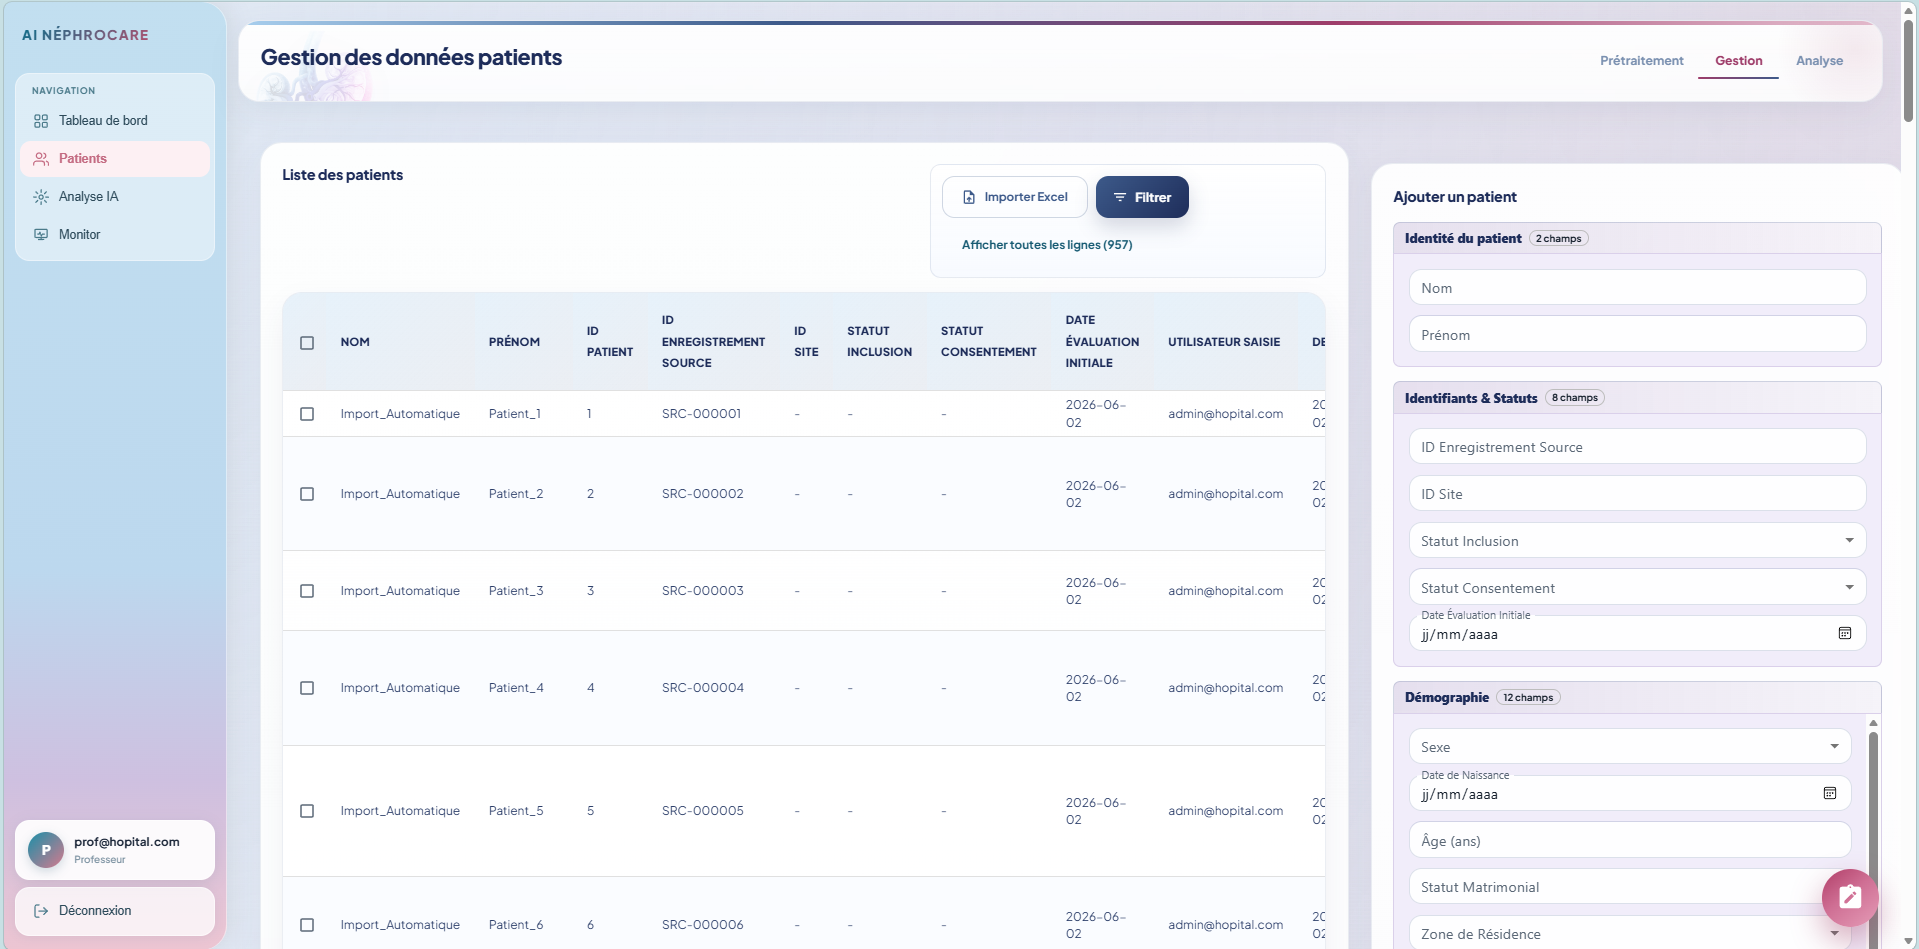
\includegraphics[width=0.85\textwidth]{data_mgmt_table.png}}{\framebox[0.85\textwidth][c]{\small[Screenshot: Data Management --- patient table with column mapping]}}
\caption{Data management interface --- searchable patient table with dynamic column support}
\label{fig:data_mgmt}
\end{figure}

The data management tab presents a \textbf{searchable, filterable, and sortable patient data table}. After a preprocessed file is validated and integrated, its columns are automatically \textbf{mapped to the platform's fixed column structure}:
\begin{itemize}
  \item Each column in the imported file is matched to a predefined clinical field (e.g., "Albumine basale" in the file $\rightarrow$ \texttt{albumine\_basale} in the database schema)
  \item Columns that match known field names are stored in their corresponding structured sections
  \item Columns that \textbf{do not match} any predefined field are stored in the \texttt{extra\_data} JSONB field as \textbf{dynamic columns}
\end{itemize}

\textbf{Dynamic Columns}: The platform supports columns that are not part of the fixed schema. These "dynamic columns" appear as additional columns in the patient table, are fully searchable and filterable, and are preserved across imports. This mechanism allows the platform to accommodate institution-specific variables without modifying the database schema.

\begin{figure}[htbp]
\centering
\IfFileExists{data_mgmt_dynamic_cols.png}{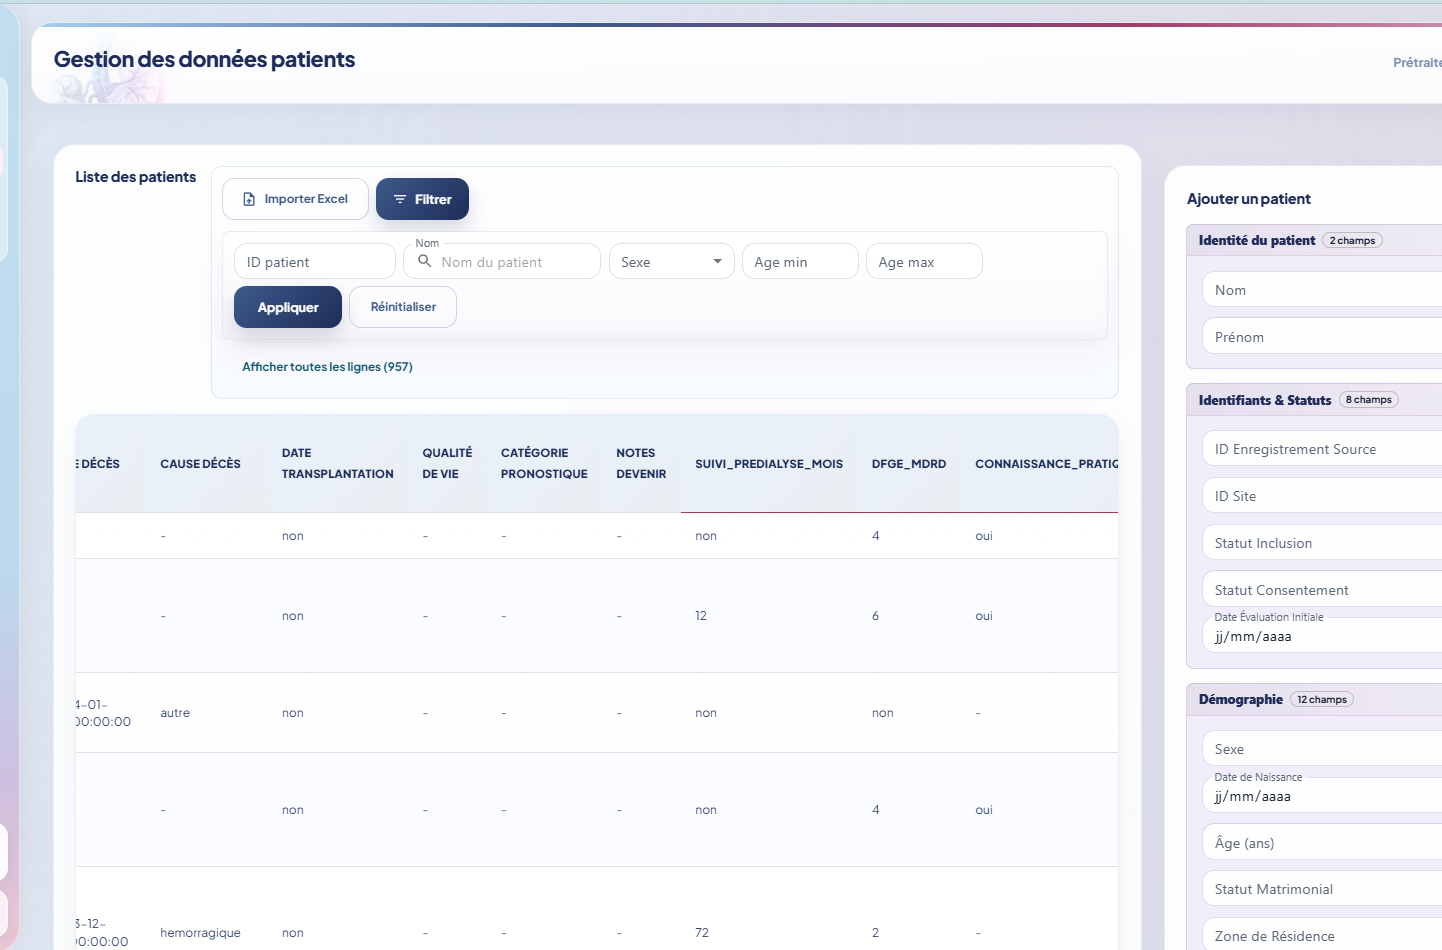
\includegraphics[width=0.85\textwidth]{data_mgmt_dynamic_cols.png}}{\framebox[0.85\textwidth][c]{\small[Screenshot: Dynamic columns visible in patient table]}}
\caption{Dynamic column support --- institution-specific variables displayed as regular table columns alongside the fixed schema}
\label{fig:data_mgmt_dynamic_cols}
\end{figure}

The data management interface provides filtering, search, and column visibility controls. A \textbf{search bar} performs full-text search across all patient fields, a \textbf{column visibility toggle} shows or hides specific columns, and a \textbf{filter panel} allows filtering by any field value.

\begin{figure}[htbp]
\centering
\IfFileExists{data_mgmt_filter.png}{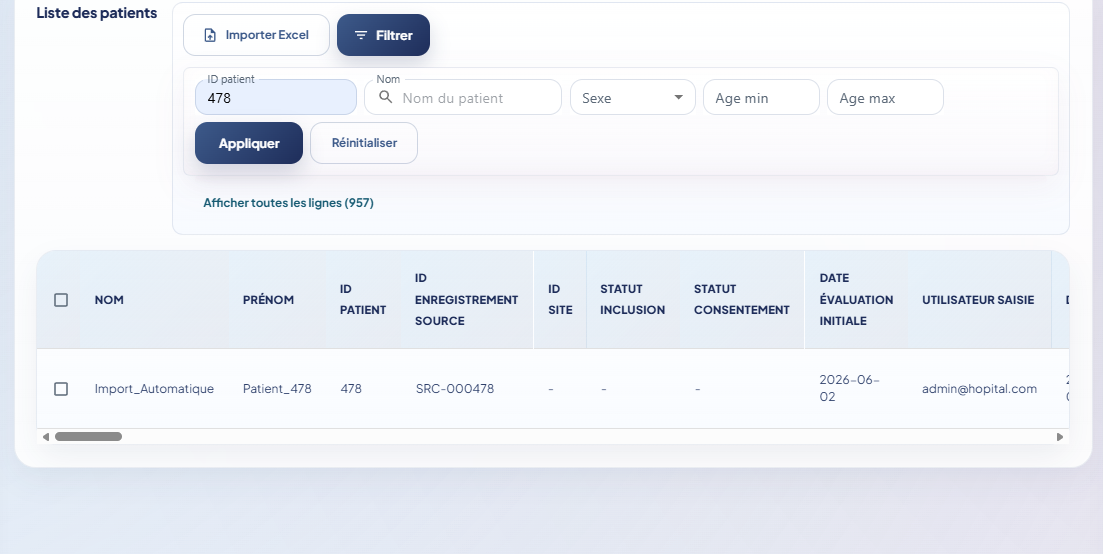
\includegraphics[width=0.85\textwidth]{data_mgmt_filter.png}}{\framebox[0.85\textwidth][c]{\small[Screenshot: Data Management filter panel]}}
\caption{Data management filter panel --- multi-field filtering with active filter indicators}
\label{fig:data_mgmt_filter}
\end{figure}

Patient records can be created, modified, and deleted through dedicated actions: an \textbf{Add patient} button opens a blank entry form, an \textbf{Edit} button opens the full 160+ field record for inline modification, and a \textbf{Delete} button removes the record after confirmation.

\begin{figure}[htbp]
\centering
\IfFileExists{data_mgmt_edit.png}{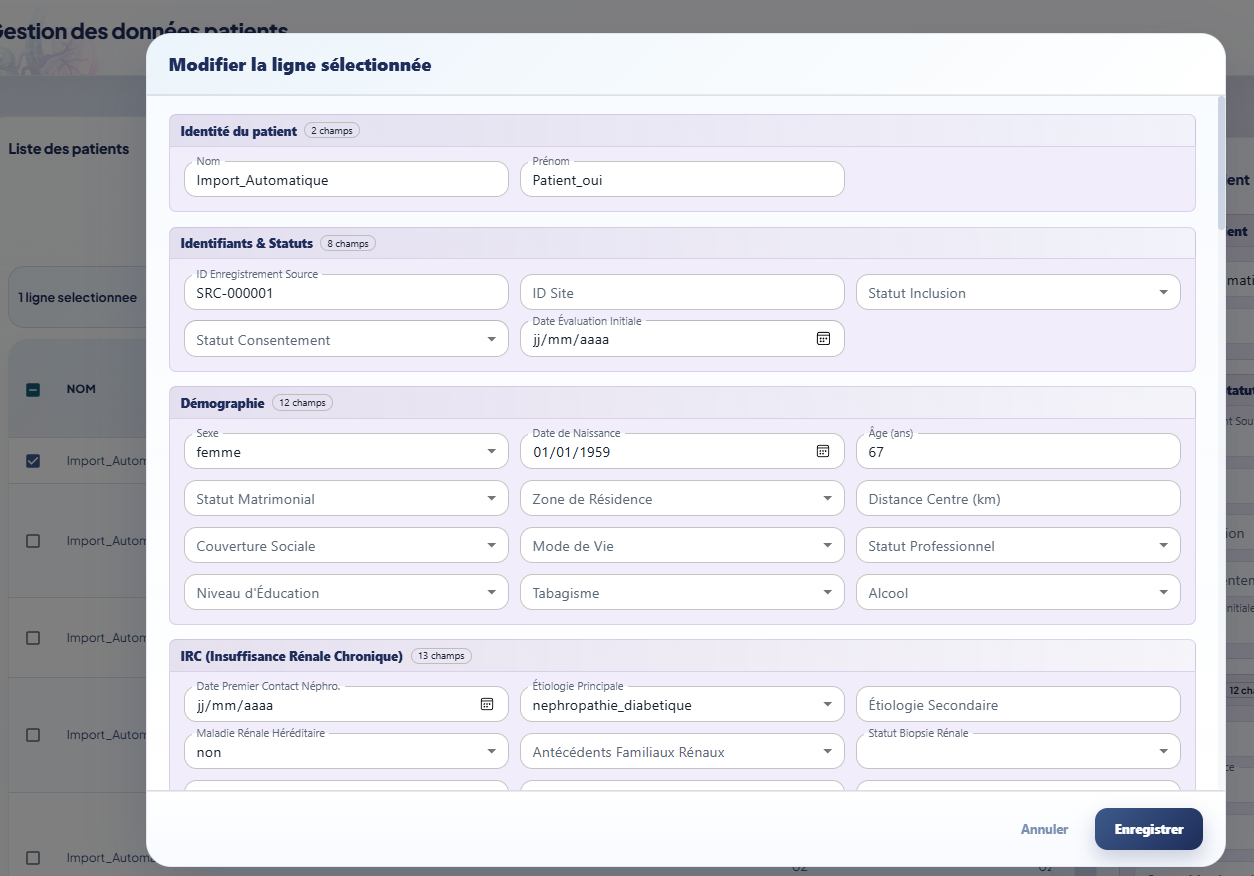
\includegraphics[width=0.85\textwidth]{data_mgmt_edit.png}}{\framebox[0.85\textwidth][c]{\small[Screenshot: Patient record edit form]}}
\caption{Patient record edit form --- all 160+ clinical variables organized in collapsible sections}
\label{fig:data_mgmt_edit}
\end{figure}

Bulk data operations are supported via an \textbf{Import} button (Excel/CSV upload with column mapping) and an \textbf{Export} button (downloads all visible data as .xlsx). Dynamic columns imported from external files are listed in a dedicated management panel where each column shows its source file and can be individually removed.

\begin{figure}[htbp]
\centering
\IfFileExists{data_mgmt_dynamic_form.png}{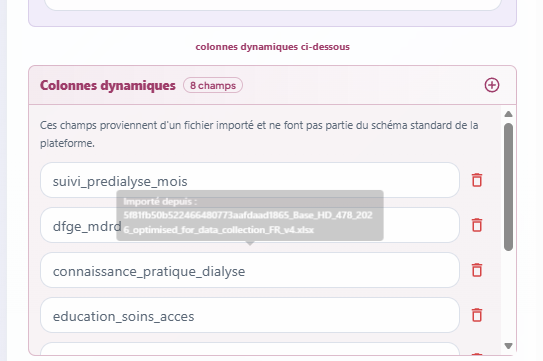
\includegraphics[width=0.72\textwidth]{data_mgmt_dynamic_form.png}}{\framebox[0.72\textwidth][c]{\small[Screenshot: Dynamic columns management panel]}}
\caption{Dynamic columns management --- list of active dynamic columns imported from Excel/CSV with their source file tooltip and individual delete action}
\label{fig:data_mgmt_dynamic_form}
\end{figure}

\subsubsection*{Tab 3 --- Analysis (Statistics)}

\begin{figure}[htbp]
\centering
\IfFileExists{analysis_charts.png}{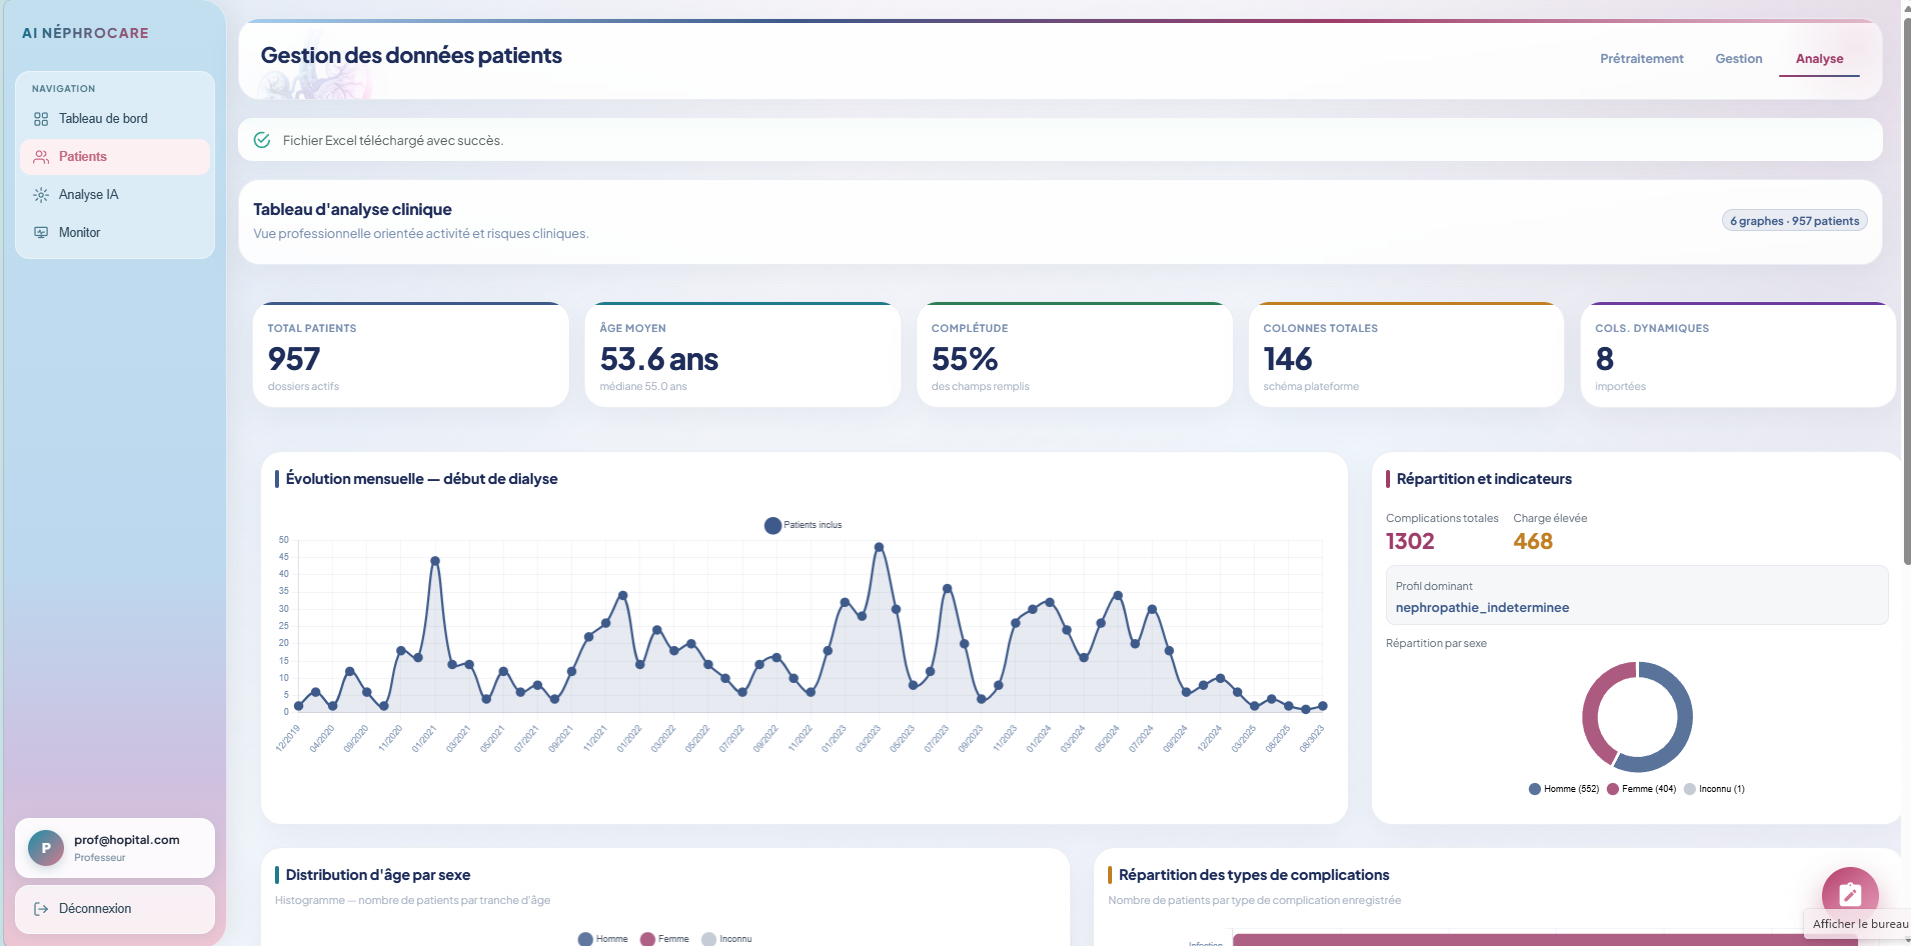
\includegraphics[width=0.85\textwidth]{analysis_charts.png}}{\framebox[0.85\textwidth][c]{\small[Screenshot: Analysis tab --- statistical charts]}}
\caption{Patient analysis interface --- epidemiological and clinical statistics charts}
\label{fig:analysis_charts}
\end{figure}

The analysis tab provides a set of interactive statistical charts generated automatically from the patient database. These charts offer an epidemiological overview of the cohort and support clinical research and reporting. [See Section~\ref{sec:dataviz} for chart descriptions.]

  \item[\textbf{AI Model} (\texttt{/modele-ai})] The AI Model section is organized into three tabs: \textit{Analysis Dashboard}, \textit{Patients}, and \textit{Prediction}.

\subsubsection*{Tab 1 --- Analysis Dashboard}

\begin{figure}[htbp]
\centering
\IfFileExists{screen/AI Model analysis dashb.png}{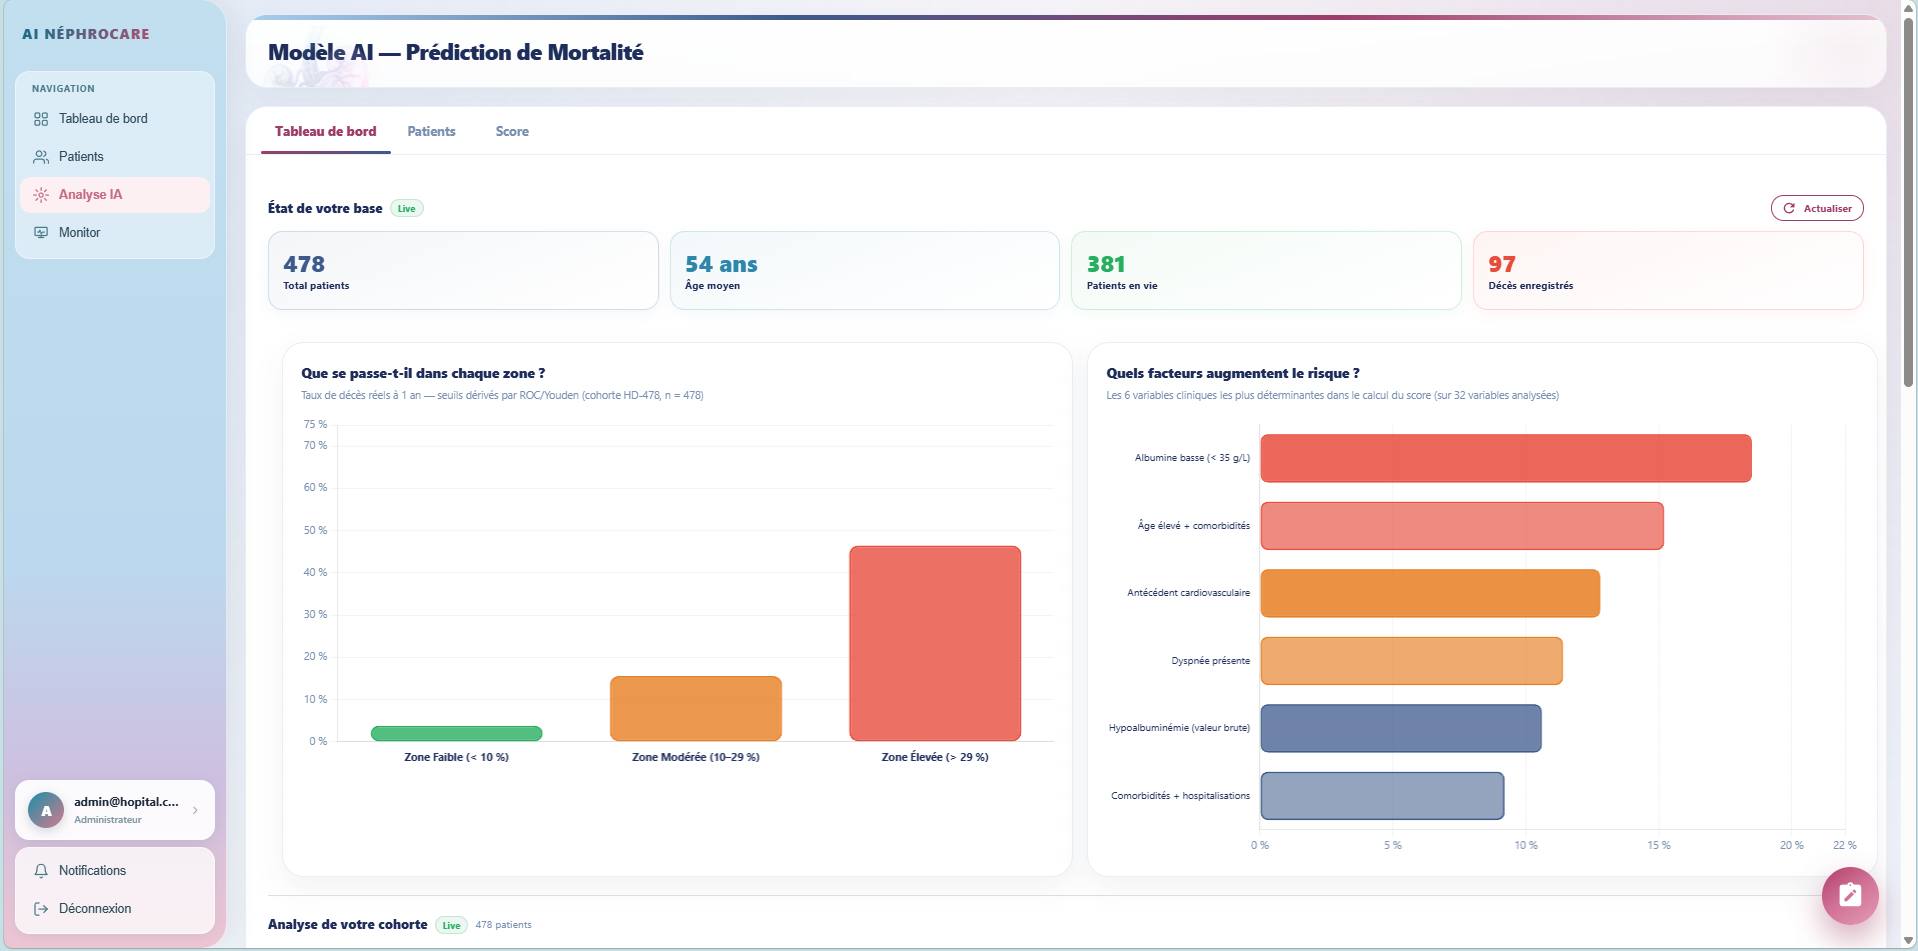
\includegraphics[width=0.85\textwidth]{screen/AI Model analysis dashb.png}}{\framebox[0.85\textwidth][c]{\small[Screenshot: AI Model analysis dashboard]}}
\caption{AI Model analysis dashboard --- SVM performance metrics and risk zone overview}
\label{fig:ai_dashboard}
\end{figure}

The analysis dashboard provides a global overview of the AI model's performance and the current state of predictions in the cohort. It displays:
\begin{itemize}
  \item \textbf{Model performance KPIs}: AUC-ROC, PR-AUC, F1-score, and Brier Score displayed as prominently colored cards
  \item \textbf{Risk zone distribution chart}: pie/doughnut chart showing the proportion of patients in Low, Moderate, and High risk zones
  \item \textbf{Model version and training date}: metadata on the currently deployed SVM model
  \item \textbf{Clinical interpretation guide}: brief description of each risk zone and its recommended clinical action
\end{itemize}

\subsubsection*{Tab 2 --- Patients}

\begin{figure}[htbp]
\centering
\IfFileExists{ai_patients_list.png}{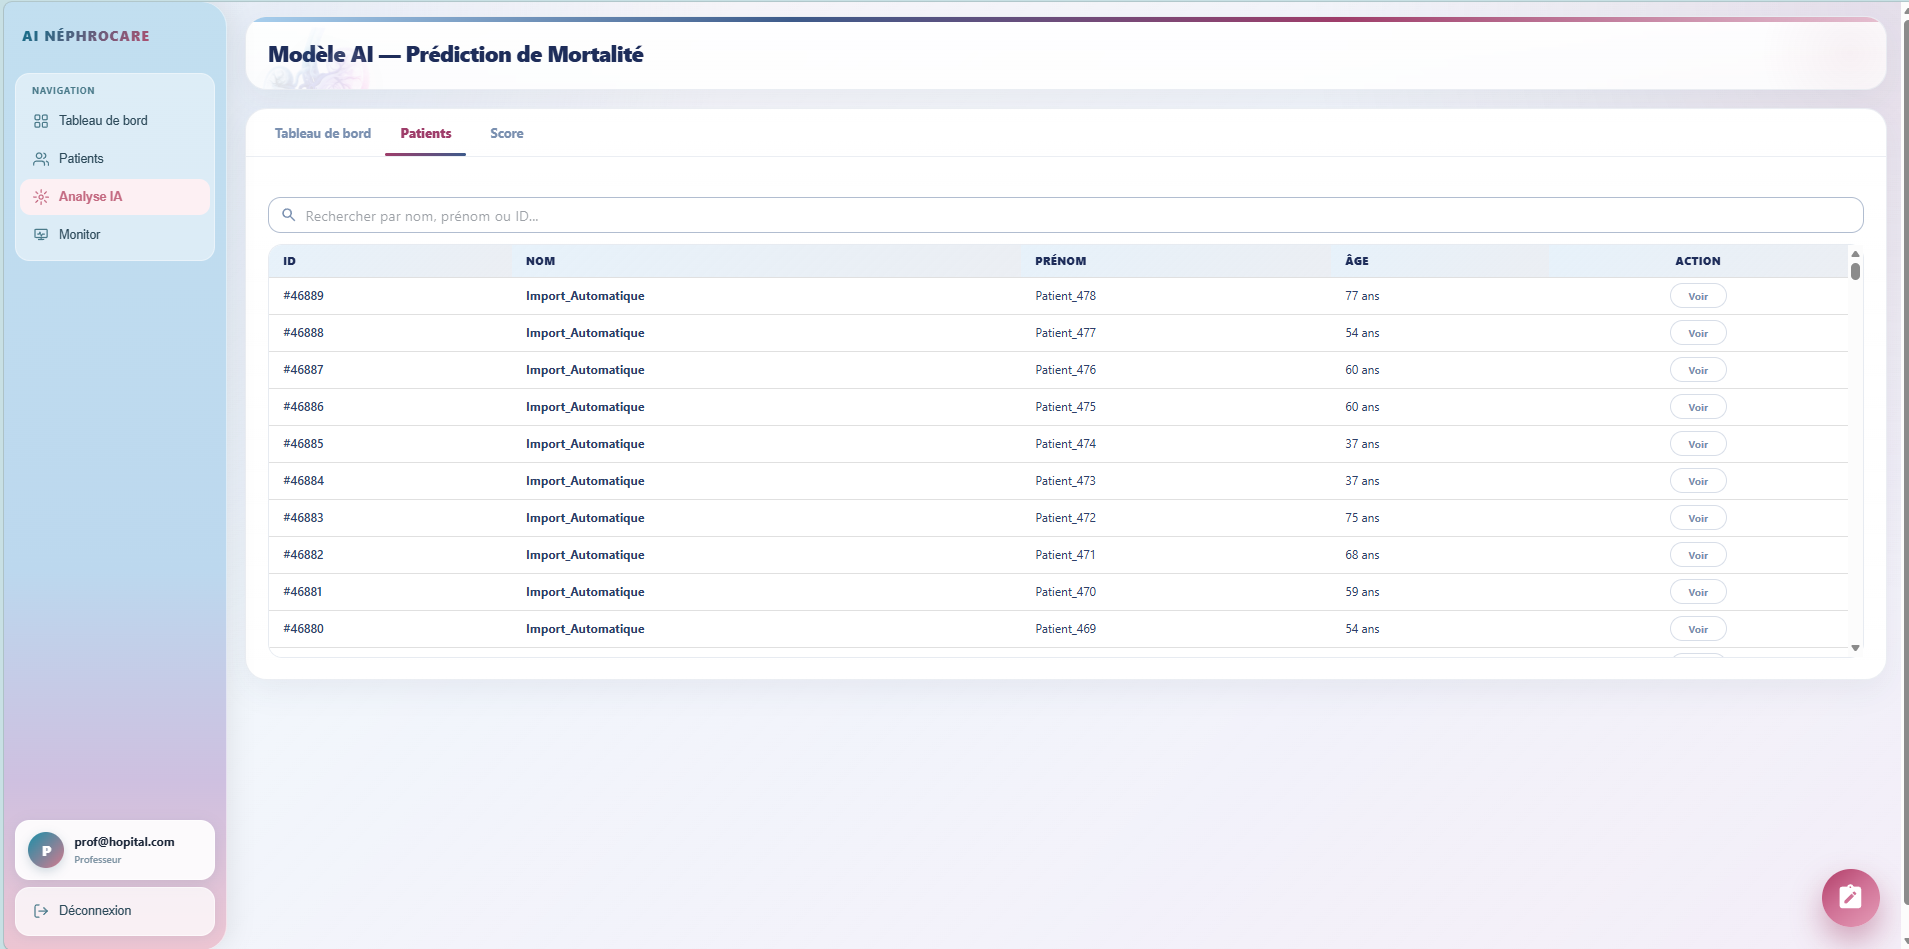
\includegraphics[width=0.85\textwidth]{ai_patients_list.png}}{\framebox[0.85\textwidth][c]{\small[Screenshot: Patient list in AI Model --- with Predict button]}}
\caption{AI Model patient list --- each row shows patient summary and a Predict action button}
\label{fig:ai_patients}
\end{figure}

The Patients tab displays the full list of patients registered in the platform. For each patient, the clinician can:
\begin{enumerate}
  \item \textbf{Select a patient} from the list to open their complete clinical dossier
  \item View the \textbf{patient dossier}: a detailed form showing all 160+ variables organized in the 11 clinical sections (Demographics, CKD history, Comorbidities, Biology, Dialysis, etc.)
  \item From the dossier, choose one of two actions:
    \begin{itemize}
      \item \textbf{Modify values and launch a simulation}: The clinician can modify any clinical parameter (e.g., reduce albumin level, change dialysis frequency) and click \textbf{"Run Simulation"}. The simulation result --- showing how the predicted mortality risk changes with the modified values --- is displayed \textbf{directly within the same Patients tab}, allowing immediate comparison without leaving the current view.

\begin{figure}[htbp]
\centering
\IfFileExists{screen/simulation.png}{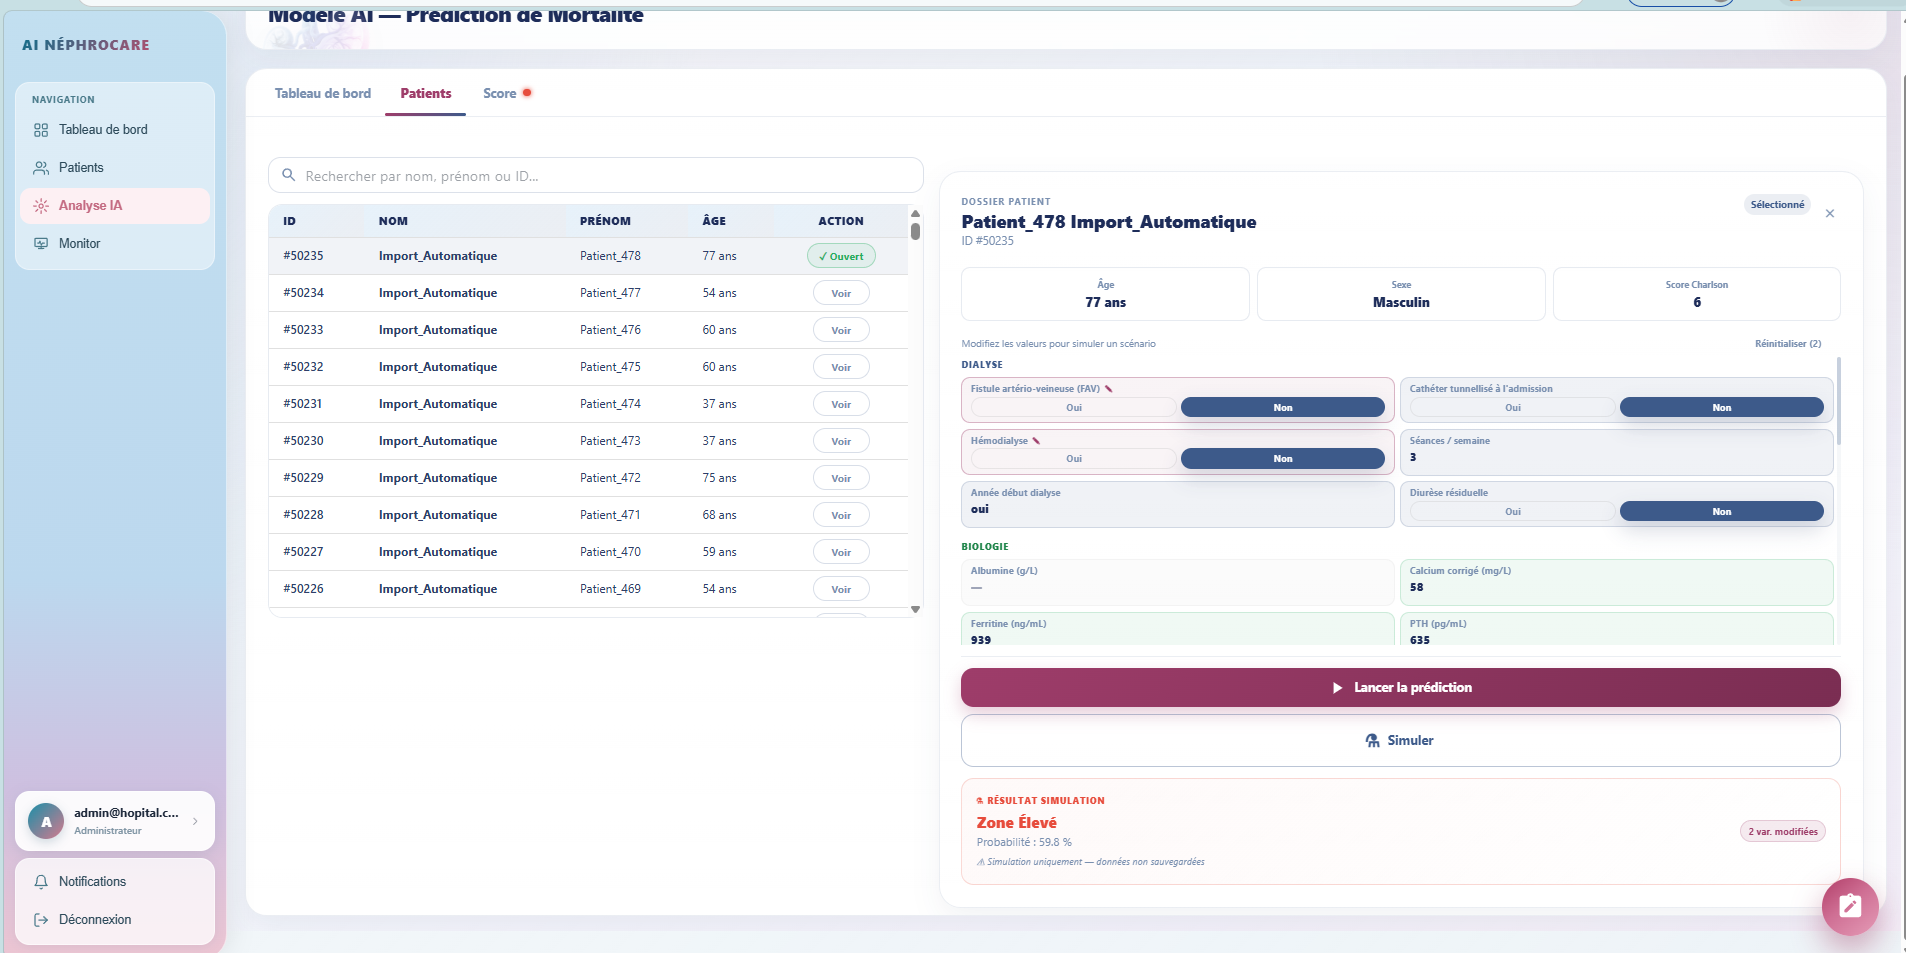
\includegraphics[width=0.85\textwidth]{screen/simulation.png}}{\framebox[0.85\textwidth][c]{\small[Screenshot: Simulation interface --- modified parameters and resulting risk prediction]}}
\caption{Clinical simulation interface --- the clinician modifies patient parameters and immediately sees the updated mortality risk prediction}
\label{fig:simulation}
\end{figure}

      \item \textbf{Launch prediction}: Using the saved clinical values already stored in the platform, click \textbf{"Predict"} to generate the official mortality risk prediction. The prediction result is displayed in the \textbf{Prediction tab} (Tab 3).
    \end{itemize}
\end{enumerate}

\subsubsection*{Tab 3 --- Prediction}

\begin{figure}[htbp]
\centering
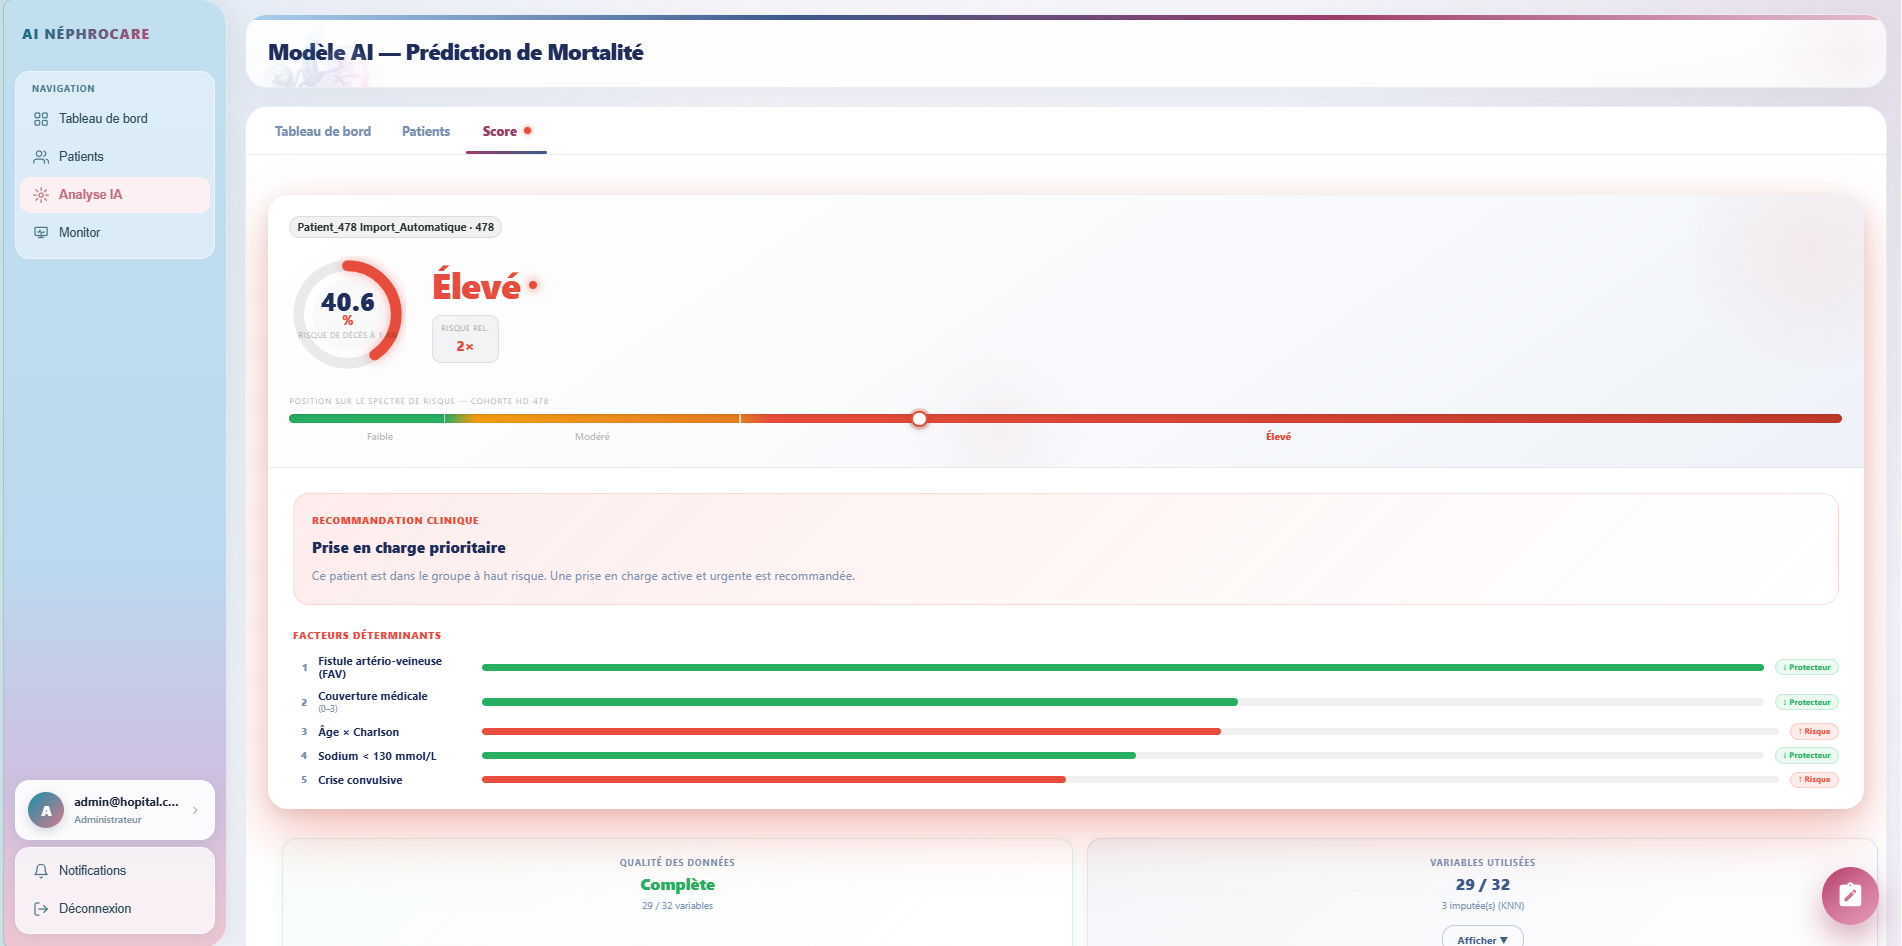
\includegraphics[width=0.85\textwidth]{screen/AI_prediction_result_risk_gauge.png}
\caption{AI prediction result interface --- risk zone gauge, calibrated probability, contributing factors, and clinical recommendation}
\label{fig:ai_prediction}
\end{figure}

The Prediction tab displays the complete mortality risk assessment for the selected patient:
\begin{itemize}
  \item \textbf{Risk gauge}: A color-coded arc gauge (green = Low, orange = Moderate, red = High) showing the calibrated probability visually
  \item \textbf{Calibrated probability}: The exact one-year mortality probability (e.g., "47.1\% estimated 1-year mortality risk")
  \item \textbf{Relative risk badge}: The risk relative to the cohort baseline (e.g., $\times$10.9)
  \item \textbf{Top-5 contributing factors}: A ranked list of the five clinical variables most influencing the prediction, with their SVM feature weights displayed as horizontal progress bars. Each factor is labeled with its direction (risk-increasing or risk-decreasing).
  \item \textbf{Clinical recommendation}: A tailored text recommendation adapted to the predicted risk zone, specifying the recommended follow-up frequency and clinical actions.
  \item \textbf{Patient information summary}: Key clinical indicators displayed alongside the prediction for context.
\end{itemize}

  \item[\textbf{Monitoring} (\texttt{/monitor})] The Patient Monitoring Board provides longitudinal follow-up of individual hemodialysis patients. The interface is split into two panels:

\begin{itemize}
  \item \textbf{Left panel — Patient list}: A searchable list of all patients in the database. The search bar accepts full-text queries across patient identifiers and names. Clicking a patient selects them and loads their complete monitoring view in the right panel.
  \item \textbf{Right panel — Clinical timeline}: An interactive chronological timeline of all clinical events recorded for the selected patient, fetched from the audit log and prediction history. Events are categorized and color-coded by type:
  \begin{itemize}
    \item \textbf{Modifications} (patient data edits) — field-level old/new value diff, displayed as structured change entries
    \item \textbf{Predictions} — each mortality risk prediction with its score, risk zone, relative risk, and top contributing factors
    \item \textbf{Imports} — preprocessing file validations, approval or rejection events
  \end{itemize}
\end{itemize}

For each prediction event in the timeline, the panel displays:
\begin{itemize}
  \item The calibrated probability and risk zone badge (Low / Moderate / High)
  \item The relative risk multiplier ($\times$RR vs.\ cohort baseline)
  \item The top-5 contributing clinical factors with their SVM weights
  \item The clinical recommendation text associated with the predicted zone
\end{itemize}

The most recent prediction is also highlighted at the top of the right panel as a \textbf{latest prediction summary card}. Date/time values are localized according to the active platform language (\texttt{fr-FR} or \texttt{en-US}).

\begin{figure}[htbp]
\centering
\IfFileExists{monitor_board.png}{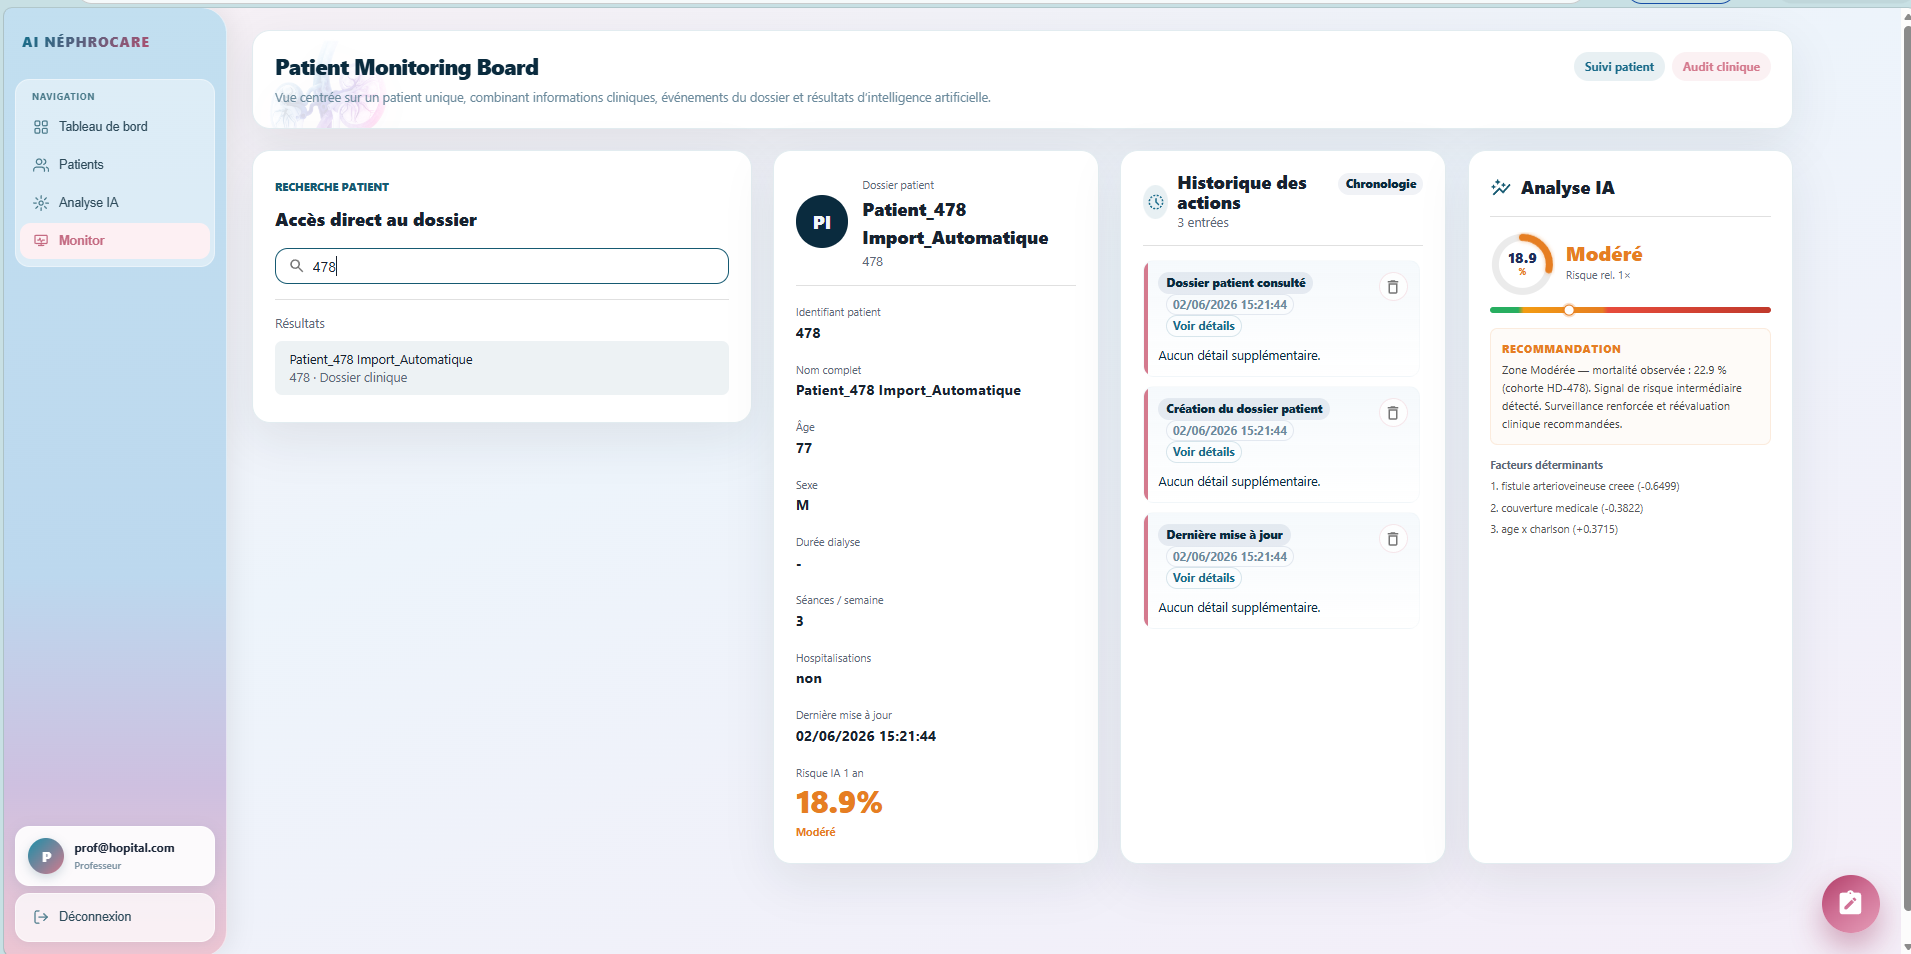
\includegraphics[width=0.85\textwidth]{monitor_board.png}}{\framebox[0.85\textwidth][c]{\small[Screenshot: Patient Monitoring Board]}}
\caption{Patient monitoring board --- patient list (left), clinical timeline with prediction history and field-level audit trail (right)}
\label{fig:monitor_board}
\end{figure}

  \item[\textbf{Profile} (\texttt{/profile})] The profile page allows each authenticated user to manage their personal settings. It is organized into three panels:

\begin{itemize}
  \item \textbf{User information panel}: Displays the user's avatar (initials-based), full name, role badge (color-coded by hierarchy level), email address, and telephone number.
  \item \textbf{Password management}: A secure form allowing the user to change their password. The user must supply their current password for identity confirmation (\texttt{POST /api/auth/change-password/}), followed by the new password (minimum 8 characters) and a confirmation field. The form validates that the new password differs from the current one and that both new-password fields match before submitting.
  \item \textbf{Language preference}: A bilingual toggle allowing the user to switch the entire platform interface between \textbf{Français} and \textbf{English}. The preference is persisted to \texttt{localStorage} (\texttt{app\_language} key) via the global \texttt{LanguageContext}, which provides translated labels for all UI strings throughout the application. On the next session, the preferred language is automatically restored.
\end{itemize}

\begin{figure}[htbp]
\centering
\IfFileExists{screen/profile_page.png}{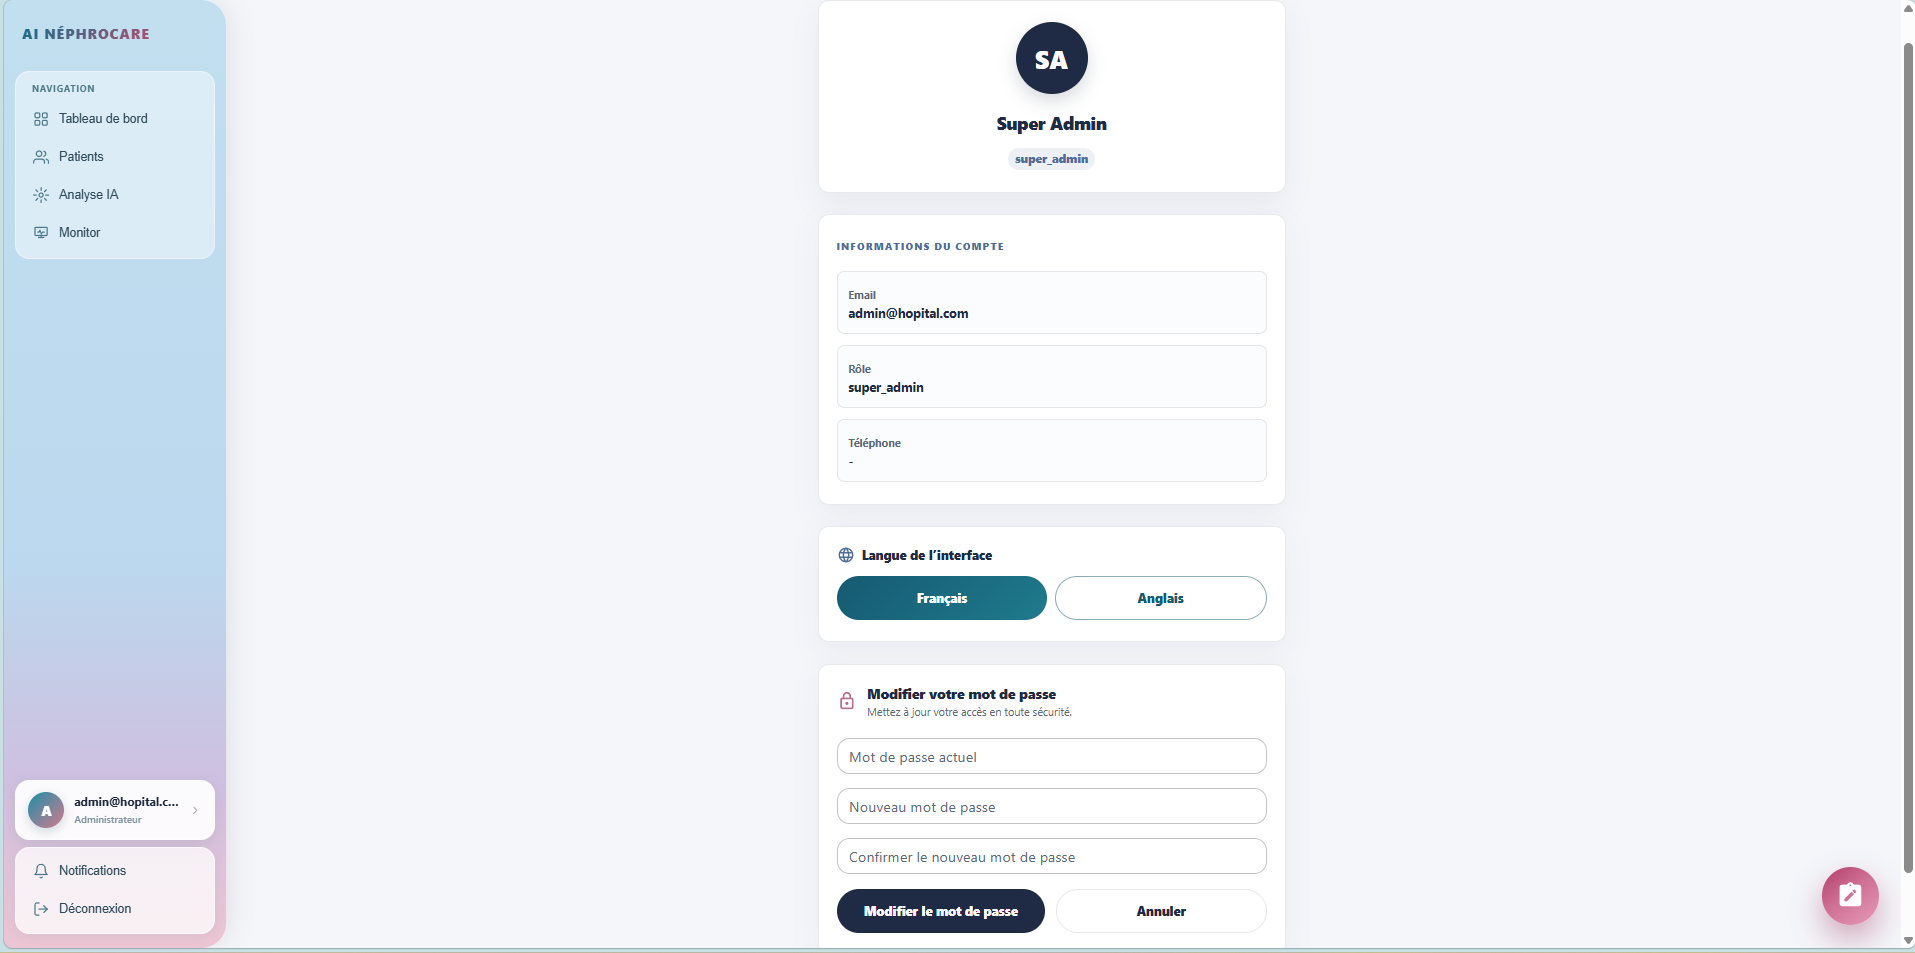
\includegraphics[width=0.85\textwidth]{profile_page.png}}{\framebox[0.85\textwidth][c]{\small[Screenshot: Profile page --- user info, password change, language selector]}}
\caption{Profile page --- user information panel, password change form, and bilingual language selector (Français / English)}
\label{fig:profile_page}
\end{figure}

\end{description}

\section{Data Visualization}\label{sec:dataviz}

\subsection{Clinical Analytics Charts (Patient Management --- Analysis Tab)}
\label{sec:dataviz_charts}

The analysis tab of the Patient Management module provides six interactive charts, each dynamically generated from the current patient database via the flat endpoint (\texttt{GET /api/patients/flat/}).

\subsubsection{Monthly Dialysis Initiation Trend}

\begin{figure}[htbp]
\centering
\IfFileExists{chart_monthly.png}{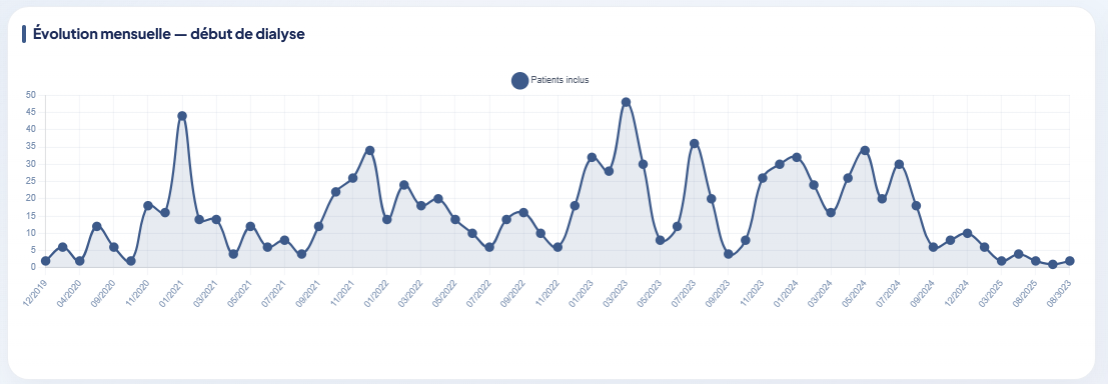
\includegraphics[width=0.85\textwidth]{chart_monthly.png}}{\framebox[0.85\textwidth][c]{\small[Screenshot: Monthly dialysis trend line chart]}}
\caption{Monthly dialysis initiation trend --- number of new patients starting hemodialysis per month}
\label{fig:chart_monthly}
\end{figure}

This line chart displays the number of patients who started hemodialysis treatment each month over the observation period (2020--2024). It allows clinical teams to identify seasonal patterns, detect increases in ESRD incidence, and plan resource allocation accordingly.

\subsubsection{Sex Distribution and Key KPIs}

\begin{figure}[htbp]
\centering
\IfFileExists{chart_sex.png}{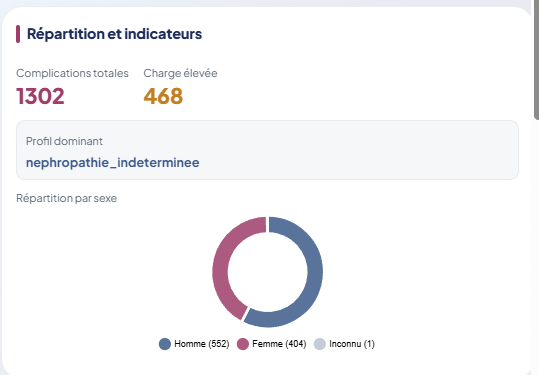
\includegraphics[width=0.85\textwidth]{chart_sex.png}}{\framebox[0.85\textwidth][c]{\small[Screenshot: Sex distribution doughnut chart]}}
\caption{Sex distribution of the hemodialysis cohort with associated KPI indicators}
\label{fig:chart_sex}
\end{figure}

This doughnut chart shows the male/female distribution of the cohort, complemented by KPI indicator cards showing the overall mean age and the data completeness rate (percentage of fields filled across all patients).

\subsubsection{Age Distribution by Sex}

\begin{figure}[htbp]
\centering
\IfFileExists{chart_age.png}{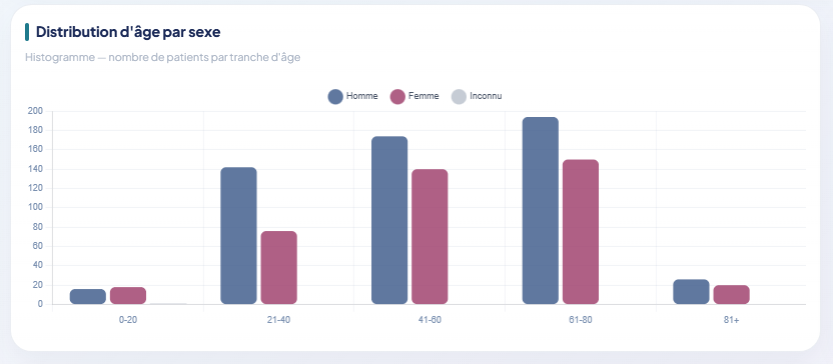
\includegraphics[width=0.85\textwidth]{chart_age.png}}{\framebox[0.85\textwidth][c]{\small[Screenshot: Age distribution grouped bar chart]}}
\caption{Age distribution of hemodialysis patients grouped by sex in 5-year age bands}
\label{fig:chart_age}
\end{figure}

A grouped bar chart displays the age distribution separately for male and female patients, using 5-year age bands. This visualization facilitates comparison of age profiles between sexes and identification of the predominant age groups requiring dialysis.

\subsubsection{Complication Type Frequencies}

\begin{figure}[htbp]
\centering
\IfFileExists{chart_complications.png}{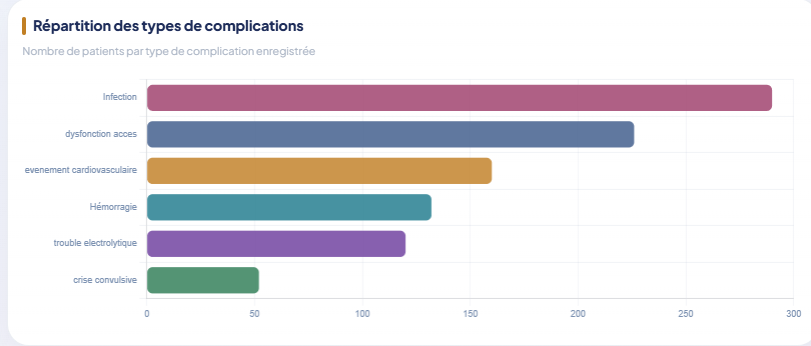
\includegraphics[width=0.85\textwidth]{chart_complications.png}}{\framebox[0.85\textwidth][c]{\small[Screenshot: Complication types horizontal bar chart]}}
\caption{Frequency of documented complication types across the patient cohort}
\label{fig:chart_complications}
\end{figure}

A horizontal bar chart ranks all documented complication types by frequency of occurrence across the cohort. This helps clinical teams identify the most prevalent complications requiring preventive or therapeutic attention.

\subsubsection{CKD Etiology by Inclusion Status}

\begin{figure}[htbp]
\centering
\IfFileExists{chart_etiology.png}{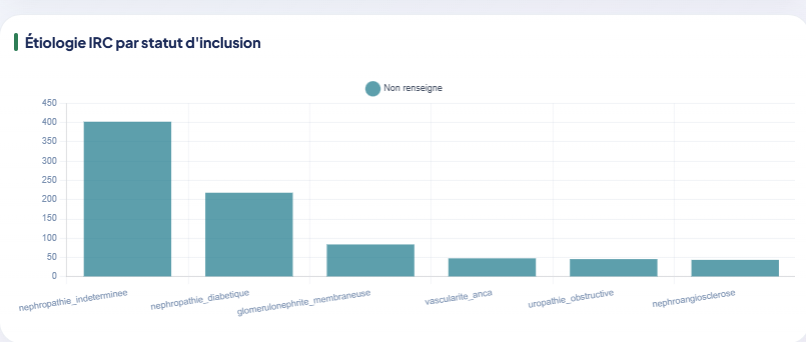
\includegraphics[width=0.85\textwidth]{chart_etiology.png}}{\framebox[0.85\textwidth][c]{\small[Screenshot: CKD etiology grouped bar chart]}}
\caption{Distribution of CKD etiologies stratified by inclusion status in the cohort}
\label{fig:chart_etiology}
\end{figure}

A grouped bar chart shows the distribution of chronic kidney disease etiologies (diabetic nephropathy, hypertensive nephropathy, glomerulonephritis, etc.) broken down by patient inclusion status. This epidemiological view supports research analyses and quality reporting.

\subsubsection{Top Comorbidity Combinations}

\begin{figure}[htbp]
\centering
\IfFileExists{chart_comorbidities.png}{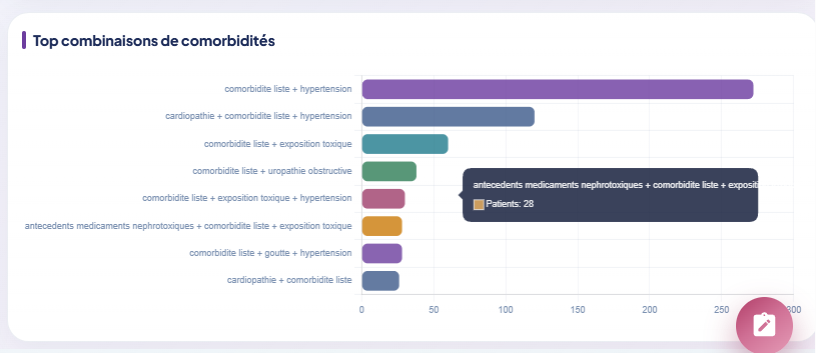
\includegraphics[width=0.85\textwidth]{chart_comorbidities.png}}{\framebox[0.85\textwidth][c]{\small[Screenshot: Comorbidity combinations horizontal bar chart]}}
\caption{Most frequent comorbidity co-occurrence combinations in the hemodialysis cohort}
\label{fig:chart_comorbidities}
\end{figure}

This horizontal bar chart identifies the most common pairs and triplets of comorbidities co-occurring in the same patient. Comorbidity clustering patterns are clinically significant, as they reflect underlying disease trajectories and influence mortality risk.

\subsection{AI Cohort Analysis Charts (AI Model --- Analysis Dashboard)}
\label{sec:dataviz_ai_charts}

The AI Model analysis dashboard includes a dedicated set of analytical charts providing deep insight into the cohort's risk stratification and the model's discriminative behavior. These charts are generated dynamically from all stored predictions via the cohort analytics endpoint.

\subsubsection{Risk Zone Distribution}

\begin{figure}[htbp]
\centering
\IfFileExists{screen/Cohort risk zone distribution.png}{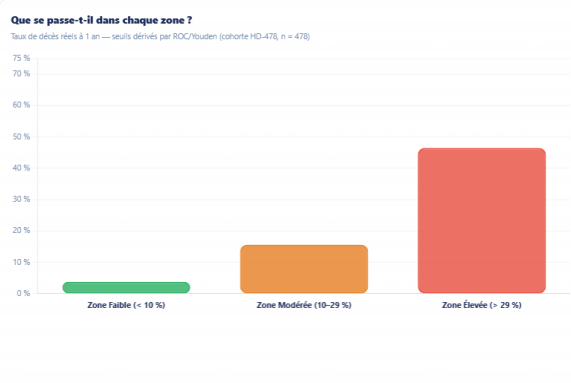
\includegraphics[width=0.75\textwidth]{screen/Cohort risk zone distribution.png}}{\framebox[0.75\textwidth][c]{\small[Screenshot: AI risk zone distribution chart]}}
\caption{Cohort risk zone distribution --- proportion of patients classified as Low, Moderate, and High risk}
\label{fig:ai_chart_zones}
\end{figure}

A doughnut/pie chart shows the proportion of the cohort falling into each risk zone (Low / Moderate / High). This high-level indicator enables the clinical team to assess the overall risk burden of their patient population at a glance.

\subsubsection{Predicted Outcome Distribution}

\begin{figure}[htbp]
\centering
\IfFileExists{screen/Devenir des patients.png}{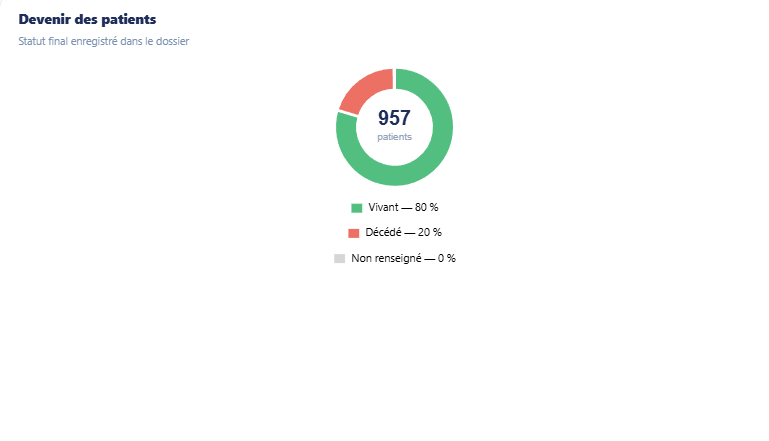
\includegraphics[width=0.80\textwidth]{screen/Devenir des patients.png}}{\framebox[0.80\textwidth][c]{\small[Screenshot: Patient outcome --- alive/deceased distribution]}}
\caption{Patient outcome distribution (alive / deceased) across the hemodialysis cohort}
\label{fig:ai_chart_outcome}
\end{figure}

This chart displays the distribution of predicted one-year mortality probabilities across the entire cohort, illustrating the range and concentration of risk scores and helping identify the proportion of patients requiring urgent clinical attention.

\subsubsection{Kaplan-Meier Survival Estimate by Risk Zone}

\begin{figure}[htbp]
\centering
\IfFileExists{screen/Kaplan-Meier.png}{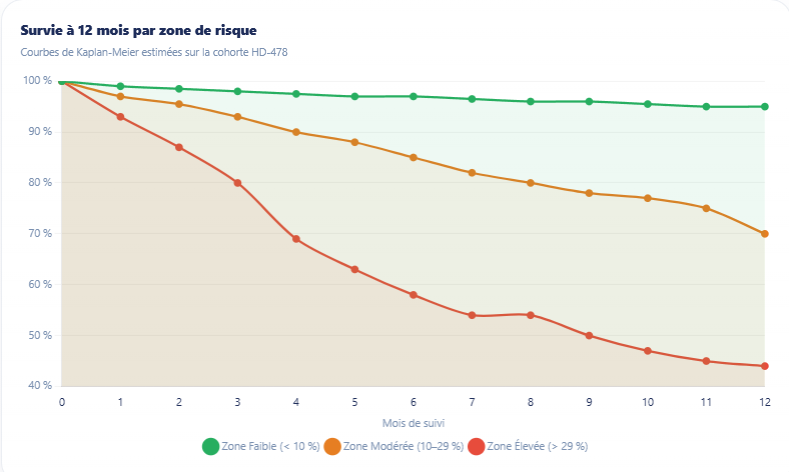
\includegraphics[width=0.82\textwidth]{screen/Kaplan-Meier.png}}{\framebox[0.82\textwidth][c]{\small[Screenshot: Kaplan-Meier survival curves by risk zone]}}
\caption{Kaplan-Meier survival curves stratified by predicted risk zone --- Low (green), Moderate (orange), High (red)}
\label{fig:ai_chart_kaplan_meier}
\end{figure}

Kaplan-Meier survival curves are plotted separately for each risk zone, illustrating the prognostic separation achieved by the model. The divergence between the three curves quantifies the clinical utility of the risk stratification: patients in the High risk zone show substantially lower survival probability over the 12-month observation window.

\subsubsection{Risk Factor Contribution Profile}

\begin{figure}[htbp]
\centering
\IfFileExists{ai_chart_factors.png}{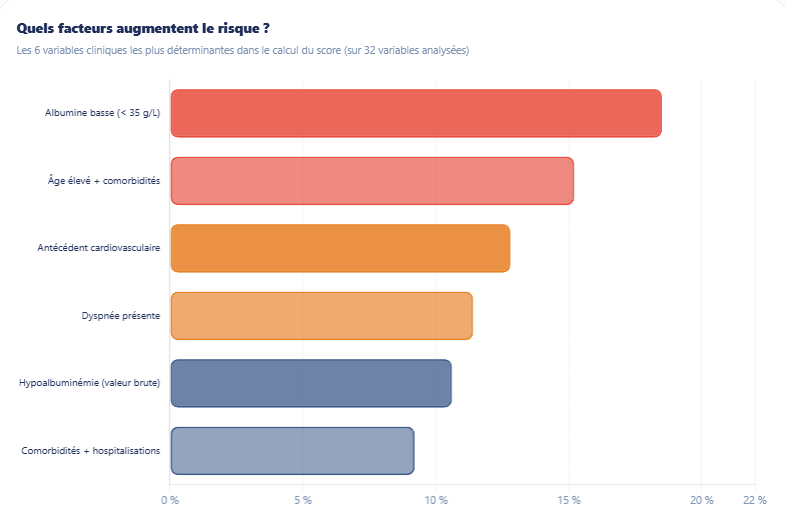
\includegraphics[width=0.82\textwidth]{ai_chart_factors.png}}{\framebox[0.82\textwidth][c]{\small[Screenshot: Top risk factors bar chart]}}
\caption{Top contributing risk factors --- mean SVM feature weights across the cohort, ranked by absolute importance}
\label{fig:ai_chart_factors}
\end{figure}

A horizontal bar chart ranks the clinical variables by their mean absolute contribution to the SVM risk score across all predictions in the cohort. Variables shown in red increase mortality risk; those in green are protective. This aggregated view complements the per-patient factor panel.

\subsubsection{Clinical Risk Profile Radar}

\begin{figure}[htbp]
\centering
\IfFileExists{ai_chart_risk_profile.png}{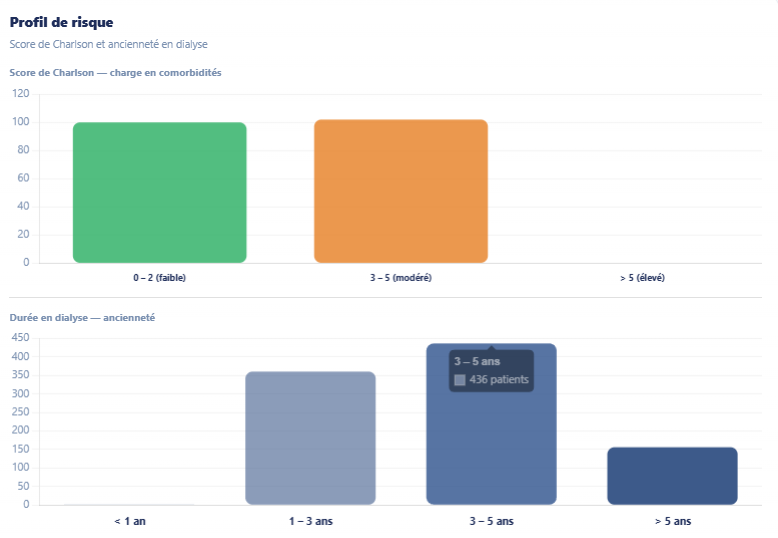
\includegraphics[width=0.72\textwidth]{ai_chart_risk_profile.png}}{\framebox[0.72\textwidth][c]{\small[Screenshot: Risk profile radar chart]}}
\caption{Multi-dimensional clinical risk profile --- radar chart of normalized key indicators for Low, Moderate, and High zones}
\label{fig:ai_chart_risk_profile}
\end{figure}

A radar (spider) chart overlays the mean clinical profile of patients in each risk zone across the six most discriminating variables (albumin, Charlson score, dialysis vintage, sodium, hemoglobin, and ultrafiltration). The shape divergence between risk zones reveals the characteristic clinical signature of each risk category.

\subsubsection{Biological Indicators by Risk Zone}

\begin{figure}[htbp]
\centering
\IfFileExists{screen/Serum albumin distribution by risk zone.png}{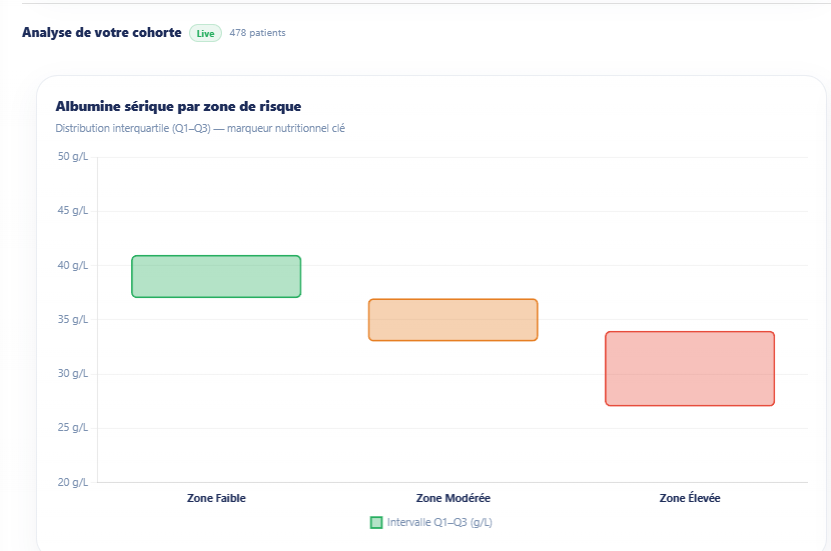
\includegraphics[width=0.85\textwidth]{screen/Serum albumin distribution by risk zone.png}}{\framebox[0.85\textwidth][c]{\small[Screenshot: Box plots of biological indicators by risk zone]}}
\caption{Serum albumin distribution by risk zone --- interquartile range (Q1--Q3) for Low, Moderate, and High zones}
\label{fig:ai_chart_boxplots_zones}
\end{figure}

This chart displays the interquartile distribution (Q1--Q3) of serum albumin across the three risk zones. The progressive decrease in albumin levels from the Low zone ($\sim$40 g/L) to the High zone ($\sim$30 g/L) confirms hypoalbuminemia as a key biological marker of elevated mortality risk in hemodialysis patients.

\section{User Workflows \& Sequence Diagrams}\label{sec:workflows}

Three sequence diagrams illustrate the principal system interactions.

%========================================================
% SEQUENCE DIAGRAM HELPER STYLE
%========================================================
% lifeline: vertical dashed line; actor: box at top; message: arrow
\tikzset{
  lifeline/.style={dashed,thick,gray!60},
  actorbox/.style={rectangle,draw,fill=darkblue!80,text=white,
                   minimum width=2.4cm,minimum height=0.55cm,
                   align=center,font=\footnotesize\bfseries},
  msgfwd/.style={-{Stealth},thick,teal!80!black},
  msgret/.style={-{Stealth},dashed,thick,orange!70!black},
  msglbl/.style={font=\tiny,above,midway},
  actbox/.style={rectangle,draw,fill=teal!20,minimum width=0.25cm,
                 minimum height=#1,inner sep=0pt}
}

%========================================================
% SEQUENCE 1 — AUTHENTICATION
%========================================================
\subsection{Sequence Diagram 1: User Authentication}

Figure~\ref{fig:seq_auth} illustrates the complete JWT authentication flow. The process begins when the user enters credentials in the browser interface. The React frontend transmits them securely to the Django API, which queries the PostgreSQL database to verify the user record and validate the password hash. Upon successful authentication, the API returns a signed JWT access token (valid 8 hours) and a refresh token (valid 1 day). The frontend decodes the access token locally to extract user information (id, email, nom, prenom, role). Subsequent API requests include the access token in the Authorization header; when the access token expires, the client uses the stored refresh token to obtain a new one via \texttt{POST /api/auth/token/refresh/}.

\begin{figure}[htbp]
\centering
\resizebox{0.92\textwidth}{!}{%
\begin{tikzpicture}
% --- Actors (top boxes) ---
\node[actorbox] (A) at (0,0)    {User (Browser)};
\node[actorbox] (B) at (3.5,0)  {React\\Frontend};
\node[actorbox] (C) at (7,0)    {Django API};
\node[actorbox] (D) at (10.5,0) {PostgreSQL};

% --- Lifelines ---
\draw[lifeline] (A.south) -- ++(0,-8.5);
\draw[lifeline] (B.south) -- ++(0,-8.5);
\draw[lifeline] (C.south) -- ++(0,-8.5);
\draw[lifeline] (D.south) -- ++(0,-8.5);

% --- Messages ---
\draw[msgfwd] (0,-0.9)  -- node[msglbl]{1. Enter email + password} (3.5,-0.9);
\draw[msgfwd] (3.5,-1.6) -- node[msglbl]{2. POST /api/auth/login/ \{email, pwd\}} (7,-1.6);
\draw[msgfwd] (7,-2.3)  -- node[msglbl]{3. SELECT WHERE email=...} (10.5,-2.3);
\draw[msgret] (10.5,-3.0) -- node[msglbl]{4. User record} (7,-3.0);
\draw[msgfwd] (7,-3.7)  -- node[msglbl,above,xshift=1.2cm]{5. verify\_password\_hash()} (7,-3.7);
  \draw[msgfwd] (7.13,-3.5) arc(90:-270:0.25cm); % self-call arrow
\draw[msgret] (7,-4.4)  -- node[msglbl]{6. \{access\_token, refresh\_token\}} (3.5,-4.4);
\draw[msgfwd] (3.5,-5.1) -- node[msglbl]{7. Store tokens in localStorage} (3.5,-5.1);
  \draw[msgfwd] (3.63,-4.9) arc(90:-270:0.25cm);
\draw[msgret] (3.5,-5.8) -- node[msglbl]{8. Redirect $\rightarrow$ /dashboard} (0,-5.8);
\draw[msgfwd] (0,-6.5)  -- node[msglbl]{9. GET /dashboard (with Bearer token)} (3.5,-6.5);
\draw[msgret] (3.5,-7.2) -- node[msglbl]{10. Render Dashboard page} (0,-7.2);

% --- Notes ---
\node[draw,fill=yellow!20,font=\tiny,align=left,inner sep=3pt] at (8.8,-5.5)
  {JWT payload:\\id, email, nom,\\prenom, role,\\exp (8h), iat};
\end{tikzpicture}
}
\caption{Sequence Diagram 1 — JWT Authentication flow}
\label{fig:seq_auth}
\end{figure}

%========================================================
% SEQUENCE 2 — LLM PREPROCESSING
%========================================================
\subsection{Sequence Diagram 2: Patient Import \& LLM Preprocessing}

Figure~\ref{fig:seq_preproc} details the asynchronous patient import and LLM preprocessing workflow. Following file upload and parsing, a Celery worker takes over the heavy LLM analysis task asynchronously --- preventing the HTTP request from timing out during the minutes-long Qwen2.5:14B inference. The Celery worker queries ChromaDB for relevant medical context (RAG), constructs the LLM prompt, and processes each data row. Results are stored in the database and polled by the frontend at regular intervals. The clinician reviews LLM suggestions, applies corrections, and submits for validation by the Head of Department before final database integration.

\begin{figure}[htbp]
\centering
\resizebox{\textwidth}{!}{%
\begin{tikzpicture}
% --- Actors ---
\node[actorbox] (U) at (0,0)      {Clinician};
\node[actorbox] (F) at (3,0)      {React\\Frontend};
\node[actorbox] (B) at (6.5,0)    {Django API};
\node[actorbox] (CE) at (9.5,0)   {Celery\\Worker};
\node[actorbox] (OL) at (12.5,0)  {Ollama\\(LLM)};
\node[actorbox] (CH) at (15.5,0)  {ChromaDB};
\node[actorbox] (DB) at (18.5,0)  {Filesystem / DB};

% --- Lifelines ---
\foreach \x in {0,3,6.5,9.5,12.5,15.5,18.5}
  \draw[lifeline] (\x,-0.28) -- ++(0,-13.5);

% --- Messages ---
\draw[msgfwd] (0,-0.9)  -- node[msglbl]{1. Upload Excel file} (3,-0.9);
\draw[msgfwd] (3,-1.6)  -- node[msglbl]{2. POST /api/patients/preprocess/analyze/ (multipart)} (6.5,-1.6);
\draw[msgfwd] (6.5,-2.3) -- node[msglbl]{3. Save temp file, generate session\_id (UUID)} (6.5,-2.3);
  \draw[msgfwd] (6.63,-2.1) arc(90:-270:0.25cm);
\draw[msgret] (6.5,-3.0) -- node[msglbl]{4. \{preprocess\_id\}} (3,-3.0);
\draw[msgfwd] (6.5,-3.7) -- node[msglbl]{5. analyze\_preprocess\_async(session\_id)} (9.5,-3.7);

% Async block
\draw[dashed,gray] (8.2,-4.1) rectangle (17.2,-10.3);
\node[font=\tiny\itshape,gray] at (12.7,-4.35) {async (Celery)};

\draw[msgfwd] (9.5,-4.7) -- node[msglbl]{6. Query medical context} (15.5,-4.7);
\draw[msgret] (15.5,-5.4) -- node[msglbl]{7. RAG embeddings context} (9.5,-5.4);
\draw[msgfwd] (9.5,-6.1) -- node[msglbl]{8. POST /api/generate (prompt+context)} (12.5,-6.1);
\draw[msgret] (12.5,-6.8) -- node[msglbl]{9. Cell corrections JSON} (9.5,-6.8);
\draw[msgfwd] (9.5,-7.5) -- node[msglbl]{10. Save session JSON \{status, report, corrections\}} (18.5,-7.5);
\draw[msgret] (18.5,-8.2) -- node[msglbl]{11. OK (JSON file written)} (9.5,-8.2);
\draw[msgfwd] (9.5,-8.9) -- node[msglbl]{12. Update session status = «completed» (filesystem)} (18.5,-8.9);

% Back to user
\draw[msgfwd] (3,-9.8)  -- node[msglbl]{13. GET /api/patients/preprocess/\{id\}/rows/ (polling)} (6.5,-9.8);
\draw[msgret] (6.5,-10.5) -- node[msglbl]{14. Rows + LLM suggestions} (3,-10.5);
\draw[msgret] (3,-11.2) -- node[msglbl]{15. Display cell corrections} (0,-11.2);
\draw[msgfwd] (0,-11.9) -- node[msglbl]{16. Review + override + submit validation} (3,-11.9);
\draw[msgfwd] (3,-12.6) -- node[msglbl]{17. POST /api/patients/preprocess/\{id\}/integrate/ (chef)} (6.5,-12.6);
\draw[msgfwd] (6.5,-13.1) -- node[msglbl]{18. PostgreSQL: INSERT INTO patients\_patient + AuditLog} (18.5,-13.1);

\end{tikzpicture}
}
\caption{Sequence Diagram 2 — Patient Import and LLM Preprocessing}
\label{fig:seq_preproc}
\end{figure}

%========================================================
% SEQUENCE 3 — MORTALITY PREDICTION
%========================================================
\subsection{Sequence Diagram 3: Mortality Risk Prediction}

Figure~\ref{fig:seq_predict} traces the complete workflow triggered when a clinician requests a 1-year mortality prediction for a patient. The sequence involves five actors: the clinician navigating the React frontend, the Django REST API, the PostgreSQL database, and the pre-trained SVM pipeline loaded from a \texttt{.joblib} file.

The flow begins when the clinician clicks the \textit{Predict} button (Step~1), which sends \texttt{GET /api/predictions/patient/\{patient\_id\}/mortalite/} to the backend (Step~2). The API retrieves the full patient record from PostgreSQL (Steps~3--4) and calls \texttt{extract\_features\_for\_patient()} to build the 32-feature clinical vector (Step~5). The vector is passed to the SVM pipeline (Step~6), which internally applies KNN imputation ($k=3$), Yeo-Johnson power transformation, and linear SVC, before returning the Platt-calibrated probability $\hat{p}$ via a single \texttt{predict\_proba()} call on the \texttt{CalibratedClassifierCV} (Step~7) --- there is no separate raw probability step.

The backend then derives the risk score as $\text{score} = \hat{p} \times 100$ and assigns a categorical risk level using dynamic clinical thresholds ($T_1$/$T_2$ loaded from \texttt{seuils\_classification.joblib}, defaulting to 10\%/29\%): \textbf{Low} ($\hat{p} < T_1$), \textbf{Moderate} ($T_1 \leq \hat{p} < T_2$), or \textbf{High} ($\hat{p} \geq T_2$) (Step~8). The prediction result is then saved to a JSON cache on the filesystem via \texttt{\_save\_last\_prediction()} (Step~9). The structured JSON response (Step~10) contains \texttt{risk\_level}, \texttt{risk\_score}, \texttt{mortality\_probability}, \texttt{factors}, and \texttt{recommendation}, which the frontend uses to render the risk gauge and results panel (Step~11).

\begin{figure}[htbp]
\centering
\resizebox{0.95\textwidth}{!}{%
\begin{tikzpicture}
% --- Actors ---
\node[actorbox] (U) at (0,0)     {Clinician};
\node[actorbox] (F) at (3.5,0)   {React\\Frontend};
\node[actorbox] (B) at (7,0)     {Django API};
\node[actorbox] (DB) at (10.5,0) {PostgreSQL};
\node[actorbox] (ML) at (14,0)   {SVM Pipeline};

% --- Lifelines ---
\foreach \x in {0,3.5,7,10.5,14}
  \draw[lifeline] (\x,-0.28) -- ++(0,-12);

% --- Messages ---
\draw[msgfwd] (0,-0.9)   -- node[msglbl]{1. Click «Prédire» for patient} (3.5,-0.9);
\draw[msgfwd] (3.5,-1.6) -- node[msglbl]{2. GET /api/predictions/patient/\{patient\_id\}/mortalite/} (7,-1.6);
\draw[msgfwd] (7,-2.3)   -- node[msglbl]{3. SELECT patient WHERE id=patient\_id} (10.5,-2.3);
\draw[msgret] (10.5,-3.0) -- node[msglbl]{4. Patient ORM object} (7,-3.0);
\draw[msgfwd] (7,-3.7)   -- node[msglbl]{5. extract\_features(patient) $\rightarrow$ vector[32]} (7,-3.7);
  \draw[msgfwd] (7.13,-3.5) arc(90:-270:0.25cm);
\draw[msgfwd] (7,-4.4)   -- node[msglbl]{6. pipeline.predict\_proba(X)} (14,-4.4);

% Activation box on SVM
\draw[fill=orange!20,draw=orange] (13.875,-4.7) rectangle (14.125,-7.3);
\draw[msgfwd] (14,-4.7)  -- node[msglbl,xshift=1cm]{KNNImputer(k=3)} (14,-4.7);
  \draw[msgfwd] (14.13,-4.9) arc(90:-270:0.2cm);
\draw[msgfwd] (14,-5.5)  -- node[msglbl,xshift=1.5cm]{PowerTransformer(Yeo-Johnson)} (14,-5.5);
  \draw[msgfwd] (14.13,-5.7) arc(90:-270:0.2cm);
\draw[msgfwd] (14,-6.2)  -- node[msglbl,xshift=1cm]{SVC(C=0.01, linear)} (14,-6.2);
  \draw[msgfwd] (14.13,-6.4) arc(90:-270:0.2cm);

\draw[msgret] (14,-7.3)  -- node[msglbl]{7. $\hat{p}$ $\in$ [0,1] — single predict\_proba() (Platt-scaled by CalibratedClassifierCV)} (7,-7.3);
\draw[msgfwd] (7,-8.0)   -- node[msglbl]{8. $\hat{p}<T_1$$\rightarrow$Low,\ $T_1{\leq}\hat{p}<T_2$$\rightarrow$Moderate,\ $\hat{p}{\geq}T_2$$\rightarrow$High} (7,-8.0);
  \draw[msgfwd] (7.13,-8.5) arc(90:-270:0.25cm);
\draw[msgfwd] (7,-9.4)   -- node[msglbl]{9. Save prediction to JSON cache (filesystem)} (7,-9.4);
  \draw[msgfwd] (7.13,-9.6) arc(90:-270:0.25cm);
\draw[msgret] (7,-10.5)  -- node[msglbl]{10. \{risk\_level, score, probability, factors, recommendation\}} (3.5,-10.5);
\draw[msgret] (3.5,-11.2) -- node[msglbl]{11. Display risk gauge + results} (0,-11.2);

% Zone annotation
\node[draw,fill=green!10,font=\tiny,align=left,inner sep=3pt] at (11.5,-8.7)
  {Low: $\hat{p} < T_1$ (default 0.10)\\Moderate: $T_1 \leq \hat{p} < T_2$ (default 0.29)\\High: $\hat{p} \geq T_2$};

\end{tikzpicture}
}
\caption{Sequence Diagram 3 — Mortality Risk Prediction workflow}
\label{fig:seq_predict}
\end{figure}

%============================================================
%  CHAPTER 7 — DEPLOYMENT, EVALUATION & PERSPECTIVES
%============================================================
\chapteropening{7}{Deployment, Evaluation\\[0.2cm]\& Perspectives}{Docker deployment, system testing, results, and future work.}{%
  \textbf{7.1}\hspace{8pt}Deployment Architecture \dotfill \pageref{sec:deploy}\\[3pt]
  \textbf{7.2}\hspace{8pt}System Testing \dotfill \pageref{sec:testing}\\[3pt]
  \textbf{7.3}\hspace{8pt}Performance Evaluation \dotfill \pageref{sec:perf}\\[3pt]
  \textbf{7.4}\hspace{8pt}Results \& Impact \dotfill \pageref{sec:impact}\\[3pt]
  \textbf{7.5}\hspace{8pt}Limitations \dotfill \pageref{sec:limits}\\[3pt]
  \textbf{7.6}\hspace{8pt}Future Work \dotfill \pageref{sec:future}\\[3pt]
}
\chapter{Deployment, Evaluation \& Perspectives}

\section{Deployment Architecture}\label{sec:deploy}

The platform is fully containerized using Docker Compose, enabling reproducible deployment across development and production environments.

\subsection{Docker Compose Setup}

The entire platform is packaged as a seven-service Docker Compose stack, deployed with a single command: \texttt{docker compose up --build -d}.

The Docker Compose stack is organized around seven interconnected services that form the complete AI NéphroCare system. The \texttt{medical\_db} service runs PostgreSQL 16, the primary relational database, with data persisted in a named Docker volume (\texttt{postgres\_data}) to survive container restarts. The \texttt{medical\_redis} service provides an in-memory message broker for the Celery task queue. The \texttt{medical\_backend} service contains the Django REST Framework API; it depends on both the database and Redis being healthy before starting, ensuring correct initialization order. The \texttt{medical\_frontend} service serves the pre-built React application as static files. The \texttt{medical\_ollama} service hosts the locally-deployed Qwen2.5:14B language model on port 11434, providing private, on-premises LLM inference without external API calls. Finally, \texttt{medical\_celery\_worker} and \texttt{medical\_audit\_cleanup} handle asynchronous task processing and scheduled maintenance (audit log cleanup) respectively.

\section{System Testing}\label{sec:testing}

Testing covered functional correctness, API security, and end-to-end workflows across all platform modules.

\subsection{Functional Tests}

Functional testing covered the complete user journey from authentication through clinical data management, AI prediction, and administrative operations. Tests were executed manually for each user role (Admin, Head of Department, Resident, Professor) to verify that RBAC restrictions were correctly enforced. Key test scenarios included:

\begin{itemize}
  \item \textbf{Authentication}: Login with valid/invalid credentials, token expiry handling, automatic token refresh
  \item \textbf{Patient CRUD}: Create, read, update, delete operations on patient records across all authorized roles
  \item \textbf{Excel import}: Import of the 478-patient HD cohort file --- verifying correct column mapping, dynamic column handling, and data integrity after integration
  \item \textbf{LLM preprocessing}: End-to-end preprocessing pipeline with real Qwen2.5:14B analysis on a 50-row test dataset --- verifying LLM response parsing, correction display, and user override functionality
  \item \textbf{Prediction}: Mortality risk prediction for 9 test patients with known outcomes from the validation set --- verifying correct feature extraction, risk zone assignment, and top-5 factor display
  \item \textbf{RBAC}: Systematic verification that Resident accounts cannot access validation or administration endpoints, and that Head of Department accounts cannot access admin-only user management functions
  \item \textbf{Password confirmation}: Verification that account modifications (role change, password reset) correctly require entering the user's own password before saving
\end{itemize}

\subsection{API Tests}

Automated API tests were implemented using Python's \texttt{requests} library, covering all 45 endpoints. Critical tests:
\begin{itemize}
  \item \textbf{Prediction accuracy}: Known patients from the validation set return correct risk zone
  \item \textbf{Missing features tolerance}: Prediction succeeds with up to 5 of 32 features missing
  \item \textbf{Authentication}: Protected endpoints return 401 without valid JWT
  \item \textbf{RBAC}: Resident cannot access validation endpoints (returns 403)
\end{itemize}

The API test suite covers all 45 endpoints documented in Table~\ref{tab:api_endpoints}. Each test case verifies the HTTP response code, the structure of the JSON response body, and any side effects (e.g., database state changes, audit log entries). Critical test categories include:

\begin{itemize}
  \item \textbf{Authentication boundary tests}: Confirming that all protected endpoints return HTTP 401 when called without a valid JWT, and HTTP 403 when called by a user without the required role
  \item \textbf{Prediction accuracy tests}: For 9 patients with known one-year outcomes from the HD-478 test set, the prediction endpoint is called and the returned risk zone is compared against the ground-truth outcome --- confirming clinical consistency
  \item \textbf{Robustness tests}: Prediction with up to 5 missing features (KNN imputation test), import of malformed files (error handling test), and duplicate patient detection
  \item \textbf{Concurrency test}: Simultaneous LLM preprocessing requests from two sessions --- verifying Celery correctly handles parallel async tasks
\end{itemize}

\section{Performance Evaluation}\label{sec:perf}

Performance was measured under realistic clinical usage conditions, covering prediction latency, concurrent load, and preprocessing throughput.

\subsection{Prediction Latency}

\begin{table}[htbp]
\centering
\caption{Prediction endpoint latency (measured over 100 requests)}
\label{tab:latency}
\begin{tabular}{lcc}
\toprule
\textbf{Operation} & \textbf{Mean (ms)} & \textbf{P95 (ms)} \\
\midrule
Feature extraction & 12 & 18 \\
KNN imputation & 8 & 14 \\
Yeo-Johnson + SVC & 23 & 35 \\
Risk zone assignment & 2 & 4 \\
\midrule
\textbf{Total prediction} & \textbf{48} & \textbf{76} \\
\bottomrule
\end{tabular}
\end{table}

The median end-to-end prediction latency of \textbf{48ms} is well within the $<$200ms threshold considered acceptable for interactive clinical applications.

\subsection{Data Processing Time}

\begin{itemize}
  \item Excel import (478 rows): $\sim$2.3 seconds
  \item LLM preprocessing (478 rows, async): $\sim$1--2 minutes (qwen2.5:14b, GPU-accelerated)
  \item Model training on 478 patients: $\sim$45 seconds (including 10-fold CV)
\end{itemize}

The LLM preprocessing time of 1--2 minutes for 478 rows reflects the sequential processing approach used to preserve the quality of Qwen2.5:14B analysis --- each row is processed individually with full clinical context. For routine imports of smaller datasets (10--50 new patients), the processing time is proportionally reduced to under 10 seconds. The asynchronous Celery architecture ensures that this processing time does not block the user interface: clinicians can continue using other platform features while the LLM analysis runs in the background.

\section{Results \& Impact}\label{sec:impact}

This section summarises the platform's clinical value, technical achievements, and measurable outcomes relative to the initial objectives.

\subsection{Clinical Usefulness}

The three-zone risk stratification identifies:
\begin{itemize}
  \item \textbf{144 High-risk patients} (30.1\% of cohort) with 46.5\% observed mortality — enabling proactive, intensive clinical follow-up
  \item \textbf{212 Low-risk patients} (44.4\%) with only 3.8\% mortality — safely allocated to standard follow-up, optimizing resource use
\end{itemize}

The three-zone stratification — Low ($\hat{p}<10\%$), Moderate ($10\%\leq\hat{p}<29\%$), High ($\hat{p}\geq29\%$) — with thresholds derived by ROC/Youden bootstrap analysis, was confirmed clinically meaningful for daily triage and resource allocation.

These results are consistent with the KDIGO 2012 clinical practice guidelines \cite{kdigo2015}, which emphasize the importance of risk stratification in CKD management to allocate clinical resources proportionally to patient need. The platform's three-zone classification operationalizes this recommendation by translating the model's probabilistic output into three clinically actionable categories, each associated with a specific follow-up protocol.

\subsection{Decision Support Value}

Beyond risk prediction, the platform provides:
\begin{itemize}
  \item \textbf{Interpretable decisions}: Top-5 contributing factors identify the specific clinical drivers of each patient's risk score, enabling targeted interventions.
  \item \textbf{Data centralization}: For the first time, all HD patient records are in a unified, queryable database with 160+ variables.
  \item \textbf{Intelligent preprocessing}: The LLM+RAG pipeline reduced manual data cleaning time by an estimated 70--80\% in internal testing.
  \item \textbf{Audit trail}: Complete action logging satisfies regulatory requirements for clinical AI tools.
\end{itemize}

\section{Limitations}\label{sec:limits}

Several limitations affect the current version of the platform and should be addressed in future iterations.

\subsection{Data Availability}

The 478-patient cohort is adequate for a robust univariate and multivariate analysis but limits subgroup stratification (e.g., per-etiology analysis with $<20$ patients per category). External validation on a multi-center cohort remains a priority future task.

\subsection{Model Constraints}

\begin{itemize}
  \item The SVM is trained on baseline (admission) features and does not incorporate longitudinal data (e.g., 6-month Kt/V evolution).
  \item The model outputs a population-calibrated probability, not an individual certainty — communication of uncertainty to clinicians requires training.
  \item LLM preprocessing runs on \textbf{qwen2.5:14b} with GPU acceleration (Ollama), delivering significantly faster inference than CPU-only deployments; however, GPU availability remains a constraint for resource-limited hospital environments.
\end{itemize}

\section{Future Work}\label{sec:future}

The following directions are identified as high-priority extensions to the current platform.

\subsection{Real-Time Hospital Integration}

Integration with the CHU Hassan II Hospital Information System (HIS) via HL7 FHIR (Health Level 7 / Fast Healthcare Interoperability Resources) APIs would enable automatic patient data ingestion, eliminating manual Excel imports and enabling real-time risk monitoring. HL7 FHIR is a globally adopted standard for electronic health record data exchange, developed by Health Level Seven International. It defines a set of RESTful APIs and data formats (FHIR Resources) that allow different hospital information systems to share patient data in a standardized, interoperable format. Integration via FHIR would allow AI NéphroCare to automatically receive structured patient data from the CHU Hassan II HIS, eliminating manual Excel data entry.

\subsection{Advanced Deep Learning Models}

For larger future cohorts ($>2,000$ patients), transformer-based models on longitudinal lab sequences (e.g., lab-BERT) or graph neural networks encoding comorbidity co-occurrence could improve predictive performance.

\subsection{Cohort-Driven Real-Time Training and Per-Patient Prediction}

A natural extension of the current platform is to allow any user to import their own hemodialysis cohort and obtain individualized 1-year mortality predictions for each patient without any code modification. Because the entire ML pipeline — preprocessing, training, and inference — operates exclusively on the data present in the platform database, importing a new cohort automatically redefines the training corpus and produces updated, cohort-specific risk scores for every patient in that dataset. This would enable the platform to be repurposed for multicenter studies or prospective validations simply by uploading a new file.

%============================================================
%  GENERAL CONCLUSION
%============================================================
\chapter*{General Conclusion}
\addcontentsline{toc}{chapter}{General Conclusion}

This project presented the design, development, and validation of \textbf{AI NéphroCare}, a full-stack intelligent clinical decision support platform for one-year mortality prediction in hemodialysis patients at CHU Hassan II of Fès, Morocco.

The work addressed four interconnected challenges: (1) \textit{data centralization} — replacing fragmented, heterogeneous records with a structured 160+-field database; (2) \textit{data quality} — deploying an LLM+RAG preprocessing pipeline that automatically detects and corrects clinical data quality issues; (3) \textit{predictive modeling} — systematically comparing nine machine learning algorithms and selecting a linear SVM (AUC-ROC = 0.826, F1 = 0.567) with F1-optimized thresholding and three clinical risk zones; and (4) \textit{clinical usability} — embedding the model in a React-based clinical interface with interpretable results, audit trail, and role-based access control.

The key finding is that a relatively simple, well-regularized linear SVM with carefully engineered features outperforms more complex ensemble methods on this small-scale, imbalanced cohort — a result consistent with the broader ML literature on clinical prediction with limited sample sizes. The three-zone risk stratification — Low ($\hat{p}<10\%$, 3.8\% observed mortality), Moderate ($10\%\leq\hat{p}<29\%$, 15.6\%), High ($\hat{p}\geq29\%$, 46.5\%) — provides actionable clinical guidance, with thresholds grounded in TRIPOD/DOPPS/KDIGO guidelines and a relative risk ratio of $\times$12.9 between extreme zones.

From a software engineering perspective, the integration of all pipeline components — LLM preprocessing, ML inference, database management, and clinical UI — into a single Docker Compose stack demonstrates the feasibility of deploying sophisticated clinical AI tools in resource-constrained hospital environments without specialized MLOps infrastructure.

Future directions include multi-center external validation, integration with FHIR-compatible hospital systems, and exploration of deep learning models for longitudinal prediction as the cohort grows.

%============================================================
%  REFERENCES
%============================================================
\bibliographystyle{plainnat}
\begin{thebibliography}{99}

\bibitem{who2021digital}
World Health Organization (2021).
\newblock \textit{Global strategy on digital health 2020--2025}.
\newblock WHO Press, Geneva.

\bibitem{bright2012}
Bright TJ, Wong A, Dhurjati R, et al. (2012).
\newblock Effect of clinical decision-support systems: a systematic review.
\newblock \textit{Annals of Internal Medicine}, 157(1):29--43.

\bibitem{jager2019ckd}
Jager KJ, Kovesdy C, Langham R, Rosenberg M, Jha V, Zoccali C (2019).
\newblock A single number for advocacy and communication---worldwide more than 850 million individuals have kidney diseases.
\newblock \textit{Kidney International}, 96(5):1048--1050.
\newblock PMID: 31655763. DOI: 10.1016/j.kint.2019.07.012.

\bibitem{kdigo2015}
KDIGO CKD Work Group (2013).
\newblock KDIGO 2012 clinical practice guideline for the evaluation and management of chronic kidney disease.
\newblock \textit{Kidney International Supplements}, 3(1):1--150.

\bibitem{registre_rein_2022}
Réseau Épidémiologie et Information en Néphrologie (REIN) (2022).
\newblock \textit{Rapport annuel 2022 du registre REIN}.
\newblock Agence de la biomédecine, France.

\bibitem{hemodialysis_cdss_2019}
Niel O, Bastard P (2019).
\newblock Artificial intelligence in nephrology: core concepts, clinical applications, and perspectives.
\newblock \textit{American Journal of Kidney Diseases}, 74(6):803--810.
\newblock PMID: 31451330. DOI: 10.1053/j.ajkd.2019.05.020.

\bibitem{albumin_dialysis_2018}
Kalantar-Zadeh K, Kilpatrick RD, Kuwae N, et al. (2005).
\newblock Revisiting mortality predictability of serum albumin in the dialysis population: time dependency, longitudinal changes and population-attributable fraction.
\newblock \textit{Nephrology Dialysis Transplantation}, 20(9):1880--1888.
\newblock PMID: 15956056. DOI: 10.1093/ndt/gfh941.

\bibitem{llm_clinical_nlp_2023}
Qwen Team, Alibaba Cloud (2024).
\newblock Qwen2.5 Technical Report.
\newblock \textit{arXiv preprint}, arXiv:2412.15115.

\bibitem{rag_lewis_2020}
Lewis P, Perez E, Piktus A, et al. (2020).
\newblock Retrieval-augmented generation for knowledge-intensive NLP tasks.
\newblock \textit{Advances in Neural Information Processing Systems}, 33:9459--9474.

\bibitem{platt1999}
Platt JC (1999).
\newblock Probabilistic outputs for support vector machines and comparisons to regularized likelihood methods.
\newblock In A.J. Smola, P.L. Bartlett, B. Schölkopf, D. Schuurmans (eds.), \textit{Advances in Large Margin Classifiers}. MIT Press, Cambridge, MA, pp. 61--74.

\bibitem{chen_xgboost_2016}
Chen T, Guestrin C (2016).
\newblock XGBoost: A scalable tree boosting system.
\newblock \textit{Proceedings of the 22nd ACM SIGKDD}, pp. 785--794.

\bibitem{ke_lightgbm_2017}
Ke G, Meng Q, Finley T, et al. (2017).
\newblock LightGBM: A highly efficient gradient boosting decision tree.
\newblock \textit{Advances in Neural Information Processing Systems}, 30.

\bibitem{levey_mdrd_2006}
Levey AS, Coresh J, Greene T, et al. (2006).
\newblock Using standardized serum creatinine values in the Modification of Diet in Renal Disease study equation for estimating glomerular filtration rate.
\newblock \textit{Annals of Internal Medicine}, 145(4):247--254.

\bibitem{prokhorenkova_catboost_2018}
Prokhorenkova L, Gusev G, Vorobev A, et al. (2018).
\newblock CatBoost: unbiased boosting with categorical features.
\newblock \textit{Advances in Neural Information Processing Systems}, 31.

\bibitem{charlson1987}
Charlson ME, Pompei P, Ales KL, MacKenzie CR (1987).
\newblock A new method of classifying prognostic comorbidity in longitudinal studies: development and validation.
\newblock \textit{Journal of Chronic Diseases}, 40(5):373--383.
\newblock PMID: 3558716. DOI: 10.1016/0021-9681(87)90171-8.

\bibitem{yeo_johnson_2000}
Yeo IK, Johnson RA (2000).
\newblock A new family of power transformations to improve normality or symmetry.
\newblock \textit{Biometrika}, 87(4):954--959.

\bibitem{cortes_vapnik_1995}
Cortes C, Vapnik V (1995).
\newblock Support-vector networks.
\newblock \textit{Machine Learning}, 20(3):273--297.

\bibitem{breiman_rf_2001}
Breiman L (2001).
\newblock Random Forests.
\newblock \textit{Machine Learning}, 45(1):5--32.

\bibitem{geurts_et_2006}
Geurts P, Ernst D, Wehenkel L (2006).
\newblock Extremely randomized trees.
\newblock \textit{Machine Learning}, 63(1):3--42.

\bibitem{friedman_gb_2001}
Friedman JH (2001).
\newblock Greedy function approximation: a gradient boosting machine.
\newblock \textit{Annals of Statistics}, 29(5):1189--1232.

\bibitem{freund_adaboost_1997}
Freund Y, Schapire RE (1997).
\newblock A decision-theoretic generalization of on-line learning and an application to boosting.
\newblock \textit{Journal of Computer and System Sciences}, 55(1):119--139.

\bibitem{brier_1950}
Brier GW (1950).
\newblock Verification of forecasts expressed in terms of probability.
\newblock \textit{Monthly Weather Review}, 78(1):1--3.

\bibitem{zadrozny_isotonic_2002}
Zadrozny B, Elkan C (2002).
\newblock Transforming classifier scores into accurate multiclass probability estimates.
\newblock \textit{Proceedings of the 8th ACM SIGKDD}, pp. 694--699.

\bibitem{berner2007cdss}
Berner ES (2007).
\newblock \textit{Clinical Decision Support Systems: Theory and Practice}, 2nd ed.
\newblock Springer, New York.

\bibitem{shortliffe1974mycin}
Shortliffe EH, Davis R, Axline SG, et al. (1975).
\newblock Computer-based consultations in clinical therapeutics: explanation and rule acquisition capabilities of the MYCIN system.
\newblock \textit{Computers and Biomedical Research}, 8(4):303--320.

\bibitem{miller1982internist}
Miller RA, Pople HE, Myers JD (1982).
\newblock INTERNIST-1, an experimental computer-based diagnostic consultant for general internal medicine.
\newblock \textit{New England Journal of Medicine}, 307(8):468--476.

\bibitem{couchoud2009}
Couchoud C, Labeeuw M, Moranne O, et al. (2009).
\newblock A clinical score to predict 6-month prognosis in elderly patients starting dialysis for end-stage renal disease.
\newblock \textit{Nephrology Dialysis Transplantation}, 24(5):1553--1561.

\bibitem{wick2019}
Wick JP, Turin TC, Faris PD, et al. (2019).
\newblock A clinical risk prediction tool for 6-month mortality after dialysis initiation among older adults.
\newblock \textit{American Journal of Kidney Diseases}, 74(2):167--176.

\bibitem{nasr2022}
Nasr WE, Abdelhamid YA, Moustafa AA (2022).
\newblock Predicting mortality in hemodialysis patients using support vector machine.
\newblock \textit{Egyptian Journal of Internal Medicine}, 34:18.

\bibitem{sheng2020}
Sheng K, Yao X, Li J, He Y, Zhang P, Chen J (2020).
\newblock Prognostic machine learning models for first-year mortality in incident hemodialysis patients: development and validation study.
\newblock \textit{JMIR Medical Informatics}, 8(10):e20578.
\newblock PMID: 33118948. DOI: 10.2196/20578.

\bibitem{garcia2021}
Garc\'ia-Montemayor V, Martin-Malo A, Barbieri C, et al. (2021).
\newblock Predicting mortality in hemodialysis patients using machine learning analysis.
\newblock \textit{Clinical Kidney Journal}, 14(5):1388--1395.
\newblock PMID: 34221370. DOI: 10.1093/ckj/sfaa126.


\bibitem{shemin2001residual}
Shemin D, Bostom AG, Laliberty P, Dworkin LD (2001).
\newblock Residual renal function and mortality risk in hemodialysis patients.
\newblock \textit{American Journal of Kidney Diseases}, 38(1):85--90.
\newblock DOI: 10.1053/ajkd.2001.25187. URL: \url{https://www.ajkd.org/article/S0272-6386(01)14302-7/abstract}.

\bibitem{usrds2022}
United States Renal Data System (2022).
\newblock \textit{USRDS 2022 Annual Data Report: Epidemiology of Kidney Disease in the United States}.
\newblock National Institutes of Health, National Institute of Diabetes and Digestive and Kidney Diseases, Bethesda, MD.

\bibitem{khan2008score}
Khan IH, Catto GR, Edward N, Fleming LW, Henderson IS, MacLeod AM (1994).
\newblock Influence of coexisting disease on survival on renal-replacement therapy.
\newblock \textit{Lancet}, 343(8912):1511--1514.
\newblock PMID: 8094182.

\bibitem{maoujoud2017morocco}
Maoujoud O, Cherrah Y, Arrayhani M, et al. (2017).
\newblock Epidemiology, health economic context, and management of chronic kidney diseases in low and middle-income countries: the case of Morocco.
\newblock \textit{European Medical Journal}, 2(4):76--81.
\newblock DOI: 10.33590/emj/10313025.

\bibitem{brenner_kidney_2020}
Levey AS, Coresh J (2012).
\newblock Chronic kidney disease.
\newblock \textit{Lancet}, 379(9811):165--180.
\newblock PMID: 21840587. DOI: 10.1016/S0140-6736(11)60844-5.

\bibitem{collins_tripod_2015}
Collins GS, Reitsma JB, Altman DG, Moons KGM (2015).
\newblock Transparent reporting of a multivariable prediction model for individual prognosis or diagnosis (TRIPOD): the TRIPOD statement.
\newblock \textit{Annals of Internal Medicine}, 162(1):55--63.
\newblock PMID: 25560714. DOI: 10.7326/M14-0697.

\bibitem{dopps2022}
Robinson BM, Zhang J, Morgenstern H, et al. (2014).
\newblock Worldwide, mortality risk is high soon after initiation of hemodialysis.
\newblock \textit{Kidney International}, 85(1):158--165.
\newblock PMID: 23802192. DOI: 10.1038/ki.2013.252.

\bibitem{waikar2011sodium}
Waikar SS, Curhan GC, Brunelli SM (2011).
\newblock Mortality associated with low serum sodium concentration in maintenance hemodialysis.
\newblock \textit{American Journal of Medicine}, 124(1):77--84.
\newblock PMID: 21187188. PMC: PMC3040578. DOI: 10.1016/j.amjmed.2010.11.005.

\bibitem{bishop2006prml}
Bishop CM (2006).
\newblock \textit{Pattern Recognition and Machine Learning}.
\newblock Springer, New York.

\bibitem{troyanskaya2001missing}
Troyanskaya O, Cantor M, Sherlock G, et al. (2001).
\newblock Missing value estimation methods for DNA microarrays.
\newblock \textit{Bioinformatics}, 17(6):520--525.
\newblock PMID: 11395428. DOI: 10.1093/bioinformatics/17.6.520.

\bibitem{hanley1982auc}
Hanley JA, McNeil BJ (1982).
\newblock The meaning and use of the area under a receiver operating characteristic (ROC) curve.
\newblock \textit{Radiology}, 143(1):29--36.

\bibitem{kdigo_mineral_2017}
Kidney Disease: Improving Global Outcomes (KDIGO) CKD-MBD Update Work Group (2017).
\newblock KDIGO 2017 clinical practice guideline update for the diagnosis, evaluation, prevention, and treatment of chronic kidney disease--mineral and bone disorder (CKD-MBD).
\newblock \textit{Kidney International Supplements}, 7(1):1--59.

\bibitem{kdigo_anemia_2012}
Kidney Disease: Improving Global Outcomes (KDIGO) Anemia Work Group (2012).
\newblock KDIGO clinical practice guideline for anemia in chronic kidney disease.
\newblock \textit{Kidney International Supplements}, 2(4):279--335.

\bibitem{tentori2008}
Tentori F, Blayney MJ, Albert JM, et al. (2008).
\newblock Mortality risk for dialysis patients with different levels of serum calcium, phosphorus, and PTH: The Dialysis Outcomes and Practice Patterns Study (DOPPS).
\newblock \textit{American Journal of Kidney Diseases}, 52(3):519--530.
\newblock PMID: 18514987. DOI: 10.1053/j.ajkd.2008.03.020.

\bibitem{foley1998cv}
Foley RN, Parfrey PS, Sarnak MJ (1998).
\newblock Clinical epidemiology of cardiovascular disease in chronic renal disease.
\newblock \textit{American Journal of Kidney Diseases}, 32(5 Suppl 3):S112--S119.
\newblock PMID: 9820470. DOI: 10.1053/ajkd.1998.v32.pm9820470.

\bibitem{wizemann2009}
Wizemann V, Wabel P, Chamney P, et al. (2009).
\newblock The mortality risk of overhydration in haemodialysis patients.
\newblock \textit{Nephrology Dialysis Transplantation}, 24(5):1574--1579.
\newblock PMID: 19131355. DOI: 10.1093/ndt/gfn707.

\bibitem{saran2006dopps}
Saran R, Bragg-Gresham JL, Levin NW, et al. (2006).
\newblock Longer treatment time and slower ultrafiltration in hemodialysis:
  associations with reduced mortality in the DOPPS.
\newblock \textit{Kidney International}, 69(7):1222--1228.
\newblock PMID: 16609686. DOI: 10.1038/sj.ki.5000186.

\bibitem{weinhandl2010}
Weinhandl ED, Foley RN, Gilbertson DT, Arneson TJ, Snyder JJ, Collins AJ
  (2010).
\newblock Propensity-matched mortality comparison of incident hemodialysis and
  peritoneal dialysis patients.
\newblock \textit{Journal of the American Society of Nephrology},
  21(3):499--506.
\newblock PMID: 20133483. DOI: 10.1681/ASN.2009060631.

\bibitem{kalantar2005iron}
Kalantar-Zadeh K, Regidor DL, McAllister CJ, Michael B, Warnock DG (2005).
\newblock Time-dependent associations between iron and mortality in
  hemodialysis patients.
\newblock \textit{Journal of the American Society of Nephrology},
  16(10):3070--3080.
\newblock PMID: 16033854. DOI: 10.1681/ASN.2005040423.

\bibitem{liyanage2015}
Liyanage T, Ninomiya T, Jha V, et al. (2015).
\newblock Worldwide access to treatment for end-stage kidney disease: a
  systematic review.
\newblock \textit{Lancet}, 385(9981):1975--1982.
\newblock PMID: 25777665. DOI: 10.1016/S0140-6736(14)61601-9.


\end{thebibliography}

%============================================================
%  WEBOGRAPHY
%============================================================
\chapter*{Webography}
\addcontentsline{toc}{chapter}{Webography}

\begin{itemize}
  \item Django REST Framework documentation — \url{https://www.django-rest-framework.org/}
  \item React documentation — \url{https://react.dev/}
  \item scikit-learn documentation — \url{https://scikit-learn.org/stable/}
  \item Ollama project — \url{https://ollama.ai/}
  \item ChromaDB documentation — \url{https://docs.trychroma.com/}
  \item KDIGO guidelines — \url{https://kdigo.org/guidelines/}
  \item Material-UI documentation — \url{https://mui.com/}
  \item Chart.js documentation — \url{https://www.chartjs.org/}
  \item PostgreSQL 16 documentation — \url{https://www.postgresql.org/docs/16/}
  \item Docker documentation — \url{https://docs.docker.com/}
\end{itemize}

\end{document}
